% 高一26_交附闵行_周练2.tex
%   —— 高一上数学「2026-2027 年交附闵行高一上周练 2」（试卷版/答案版）
% 试卷版：xelatex 高一26_交附闵行_周练2.tex
% 答案版：xelatex "\def\isanswer{1}% 高一26_交附闵行_周练2.tex
%   —— 高一上数学「2026-2027 年交附闵行高一上周练 2」（试卷版/答案版）
% 试卷版：xelatex 高一26_交附闵行_周练2.tex
% 答案版：xelatex "\def\isanswer{1}% 高一26_交附闵行_周练2.tex
%   —— 高一上数学「2026-2027 年交附闵行高一上周练 2」（试卷版/答案版）
% 试卷版：xelatex 高一26_交附闵行_周练2.tex
% 答案版：xelatex "\def\isanswer{1}% 高一26_交附闵行_周练2.tex
%   —— 高一上数学「2026-2027 年交附闵行高一上周练 2」（试卷版/答案版）
% 试卷版：xelatex 高一26_交附闵行_周练2.tex
% 答案版：xelatex "\def\isanswer{1}\input{高一26_交附闵行_周练2.tex}"
% 紧凑版：xelatex "\def\iscompact{1}\input{高一26_交附闵行_周练2.tex}"
%
% 原始材料是微信公众号图文（公众号「魔都数学加油站」连载「27学年高一 26」，2026-09-21 发布，
% 原文标题「27学年高一26——2026-2027年上海市交附闵行高一上周练2」），
% 正文为 10 张 PNG 页（1080×1527，各页同尺寸）。原文本身就是一份**讲评版**——
% 题目下方直接印出【解析】（本卷无单独的【答案】行，填空题答案都写在解析里）。
% 试题文字与解析均照原卷录入，未改内容。卷面的粉色斜水印「魔都数学加油站」属水印，未录入。
%
% 卷首标题：原卷印作「2026-2027 年交附闵行高一上周练 2」（公众号标题里的「上海市」
% 三字卷面标题行没有，本稿照卷面），年份区间按全稿惯例排 en dash，前缀照原卷保留「年」。
%
% 与原卷的排版差异（均已在 README「说明」中交代）：
%   ① 原文自**第 3 题**起（第 1、2 题未在该文中发布），故本稿题号亦自 3 起；
%   ② 原卷本就印有「一、填空题」「二、选择题」「三、解答题」三节标题，本稿照原卷分节，
%      只把标题改排成全稿统一的「大节标题」样式；
%   ③ 原卷第 16 题的答案「D」直接印在题干末尾的括号内（原卷把括号连同 D 单独占一行），
%      第 13—15 题的括号空着、答案写在解析末句「故选 A／B／C」里；填空题的答案也都嵌在
%      解析里，本稿统一改为试卷版隐去、答案版以 \ans{} 给出（选择题另附【解析】）；
%   ④ 子集符号原卷两种并用：第 4 题题干与第 8 题、第 21(2) 题等作带下划线的 $\subseteq$，
%      第 19(2)、20(1)(2) 题作真包含的 $\subset$，本稿分别照录为 $\sub$ 与 $\subset$；
%   ⑤ 补集符号原卷作 $\complement_R$、$\complement_U$（第 4 题命题④、第 13 题选项 C、
%      第 19—20 题），本稿照录；
%   ⑥ 原卷的实数集 R 一律作斜体（第 11 题「$a\in R$」、第 14 题「$a$、$b\in R$」与解析的
%      $\{x\mid x^2+x+6>0\}=R$ 等），本稿按全稿惯例统一写作 $\R$；
%   ⑦ 原卷填空的横线约两个字宽，本稿按全稿惯例统一排 \blankline[4.4em]；
%   ⑧ 原卷未印副标题，本稿按全稿惯例补出副标题「集合与常用逻辑用语」；
%   ⑨ 第 13 题的 Venn 图原卷印在题干右侧（第 5 页），本稿移至题干之后；
%      图取原卷截图、4× LANCZOS 放大（figures/venn_ABC_lenses.png，
%      阴影为 $A\cap B$ 与 $B\cap C$ 两个交带，即 $(A\cap B)\cup(B\cap C)$）。
%
% 原卷存疑一处（照抄原卷、未改，见源码中该处上方注释）：
%   ① 第 12 题【解析】首步的方程组里印 $t<2$，而其后三处与末行答案都作 $t\leqslant2$
%      （$\left[\dfrac85,\dfrac{17}{10}\right)\cup\left(\dfrac95,2\right]$ 含 $2$）——
%      按题意 $N=\left\{x\mid t-\dfrac35\leqslant x\leqslant t\right\}\sub\{x\mid1\leqslant x\leqslant2\}$
%      只要求 $t\leqslant2$（$t=2$ 时 $N=\left[\dfrac75,2\right]$ 确实含于其中），
%      故方程组里的 $t<2$ 应是原卷笔误；本稿两处都照原卷录入、未互相迁就。
% 另：第 20(3) 题解析末两行原卷即作同话重复，照原卷录入。

\documentclass[a4paper,11pt]{article}
\usepackage{common}

\begin{document}

\examtitlest[3]{2026--2027 年交附闵行高一上周练 2}{集合与常用逻辑用语}

\bigsec{一、填空题}

\begin{enumerate}
\setcounter{enumi}{2}

\item 命题甲：集合 $M=\{x\mid kx^2-2kx+1=0\}$ 为空集；命题乙：关于 $x$ 的不等式
$x^2+(k-1)x+4>0$ 的解集为 $\R$. 若命题甲、乙中有且只有一个是真命题，则实数 $k$ 的取
值范围是 \blankline[4.4em].

\ifanswer
\solbegin
\step{因为集合 $M=\{x\mid kx^2-2kx+1=0\}$ 为空集，}
\step{当 $k\neq0$ 时，$\Delta=(-2k)^2-4k<0$，解得 $0<k<1$，}
\step{当 $k=0$ 时，方程变为 $1=0$，无解，满足题意，故 $0\leqslant k<1$；}
\step{又关于 $x$ 的不等式 $x^2+(k-1)x+4>0$ 的解集为 $\R$，}
\step{所以 $\Delta'=(k-1)^2-4\times4<0$，解得 $-3<k<5$，}
\step{当甲命题为真，乙命题为假时，无解，}
\step{当甲命题为假，乙命题为真时，$k\in(-3,0)\cup[1,5)$.}
\solend

\fi

\item 对任意 $A$、$B\sub\R$，记 $A\oplus B=\{x\mid x\in A\cup B,x\notin A\cap B\}$，
并称 $A\oplus B$ 为集合 $A$、$B$ 的对称差. 例如：若 $A=\{1,2,3\},B=\{2,3,4\}$，
则 $A\oplus B=\{1,4\}$. 下列命题中，为真命题的是 \blankline[4.4em].

\keepwithprev
①若 $A$、$B\sub\R$ 且 $A\oplus B\sub A$，则 $A\sub B$

②若 $A$、$B\sub\R$ 且 $A\oplus B=\varnothing$，则 $A=B$

③若 $A$、$B\sub\R$ 且 $A\oplus B=B$，则 $A=\varnothing$

④对任意 $A$、$B\sub\R$，都有 $A\oplus B=\complement_R A\oplus\complement_R B$

\ans{②③④}

\ifanswer
\solbegin
\step{对于①，因为 $A\oplus B\sub A$，
所以 $\{x\mid x\in A\cup B,x\notin A\cap B\}\sub A$，}
\step{故 $B\sub A$，①错误；}
\step{对于②，$A$、$B\sub\R$ 且 $A\oplus B=\varnothing$，
则 $\varnothing=\{x\mid x\in A\cup B,x\notin A\cap B\}$，}
\step{即 $A\cup B=A\cap B$，所以 $A=B$，②正确；}
\step{对于③，$A$、$B\sub\R$ 且 $A\oplus B=B$，
则 $B=\{x\mid x\in A\cup B,x\notin A\cap B\}$，}
\step{故 $A\sub B$，且 $B$ 中元素不在 $A\cap B$ 中，故 $A=\varnothing$，③正确；}
\step{对于④，$\complement_R A\oplus\complement_R B
=\{x\mid x\in\complement_R A\cup\complement_R B,x\notin\complement_R A\cap\complement_R B\}$，}
\step{其中 $\complement_R A\cup\complement_R B=\complement_R(A\cap B)$，
$\complement_R A\cap\complement_R B=\complement_R(A\cup B)$，}
\step{故 $\complement_R A\oplus\complement_R B
=\{x\mid x\in\complement_R(A\cap B),x\notin\complement_R(A\cup B)\}
=\{x\mid x\in A\cup B,x\notin A\cap B\}$，}
\step{而 $A\oplus B=\{x\mid x\in A\cup B,x\notin A\cap B\}$，
故 $A\oplus B=\complement_R A\oplus\complement_R B$，④正确.}
\step{故正确的是②③④.}
\solend

\fi

\item 已知 $A=\{a_1,a_2,a_3,a_4\},B=\{a^2\mid a\in A\}$，其中 $a_1<a_2<a_3<a_4$，
且 $a_1$、$a_2$、$a_3$、$a_4$ 均为整数，若 $A\cap B=\{a_3,a_4\},a_1+a_3=0$，
且 $A\cup B$ 中的所有元素之和为 $270$，则集合 $A$ 中所有元素之和为 \blankline[4.4em].

\ifanswer
\solbegin
\step{$A=\{a_1,a_2,a_3,a_4\},B=\{a^2\mid a\in A\}$，
因为 $A\cap B=\{a_3,a_4\},a_1+a_3=0$，}
\step{所以 $A=\{a_1,a_2,a_3,a_4\},B=\left\{a_1^2,a_2^2,a_4^2\right\}$，}
\step{若 $a_1^2=a_3$，则 $a_1=-1,a_3=1$，则 $a_2=0$，
此时 $A=\{-1,0,1,a_4\},B=\{0,1,a_4^2\}$，}
\step{因为 $A\cup B$ 中的所有元素之和为 $270$，
所以 $-1+0+1+a_4+1+a_4^2=270$，}
\step{无正整数解，舍去；}
\step{若 $a_2^2=a_3$，① $a_4^2=a_4$，所以 $a_4=1$，矛盾；}
\step{② $a_1^2=a_4$，此时 $A\cup B=\left\{-a_2^2,a_2,a_2^2,a_1^2,a_4^2\right\}$，
所以 $a_2^8+a_2^4+a_2=270$，}
\step{所以 $a_2=-2$，此时 $a_1=-4,a_2=-2,a_3=4,a_4=16$；}
\step{若 $a_4^2=a_3$，显然不成立；}
\step{综上，集合 $A$ 中所有元素之和为 $-4-2+4+16=14$.}
\solend

\fi

\item 将集合 $M=\{a_1,a_2,a_3,\cdots,a_n\}$ 分拆成两个集合 $A_i$ 和 $B_j$，且
$M\supseteq A_i\cup B_j$，$A_i\cap B_j=\varnothing$，这样的分拆方法共有 \blankline[4.4em] 种.

\ifanswer
\solbegin
\step{按集合 $A_i$ 中的元素个数进行分类：}
\step{若 $A_i$ 中有 $0$ 个元素（即 $C_n^0$ 种）时，则 $B_j$ 有 $2^n$ 种，
共有 $2^nC_n^0$ 种；}
\step{若 $A_i$ 中有 $1$ 个元素（即 $C_n^1$ 种）时，则 $B_j$ 有 $2^{n-1}$ 种，
共有 $2^{n-1}C_n^1$ 种；}
\step{若 $A_i$ 中有 $2$ 个元素（即 $C_n^2$ 种）时，则 $B_j$ 有 $2^{n-2}$ 种，
共有 $2^{n-2}C_n^2$ 种；}
\step{若 $A_i$ 中有 $3$ 个元素（即 $C_n^3$ 种）时，则 $B_j$ 有 $2^{n-3}$ 种，
共有 $2^{n-3}C_n^3$ 种；}
\step{若 $A_i$ 中有 $n$ 个元素（即 $C_n^n$ 种）时，则 $B_j$ 有 $2^0$ 种，
共有 $2^0C_n^n$ 种；}
\step{得 $2^nC_n^0+2^{n-1}C_n^1+2^{n-2}C_n^2+\cdots+2^0C_n^n=(1+2)^n$，
故这样的分拆方法有 $3^n$ 种.}
\solend

\fi

\item 已知集合 $A=\{x\mid x<2,x\in\Z\}$，$B=\{x\mid x>0,x\in\Z\}$，则
$A\cap B=$ \blankline[4.4em].

\ifanswer
\solbegin
\step{因为 $A=\{x\mid x<2,x\in\Z\}$，$B=\{x\mid x>0,x\in\Z\}$，}
\step{所以 $A\cap B=\{x\mid0<x<2,x\in\Z\}=\{1\}$.}
\solend

\fi

\item 已知集合 $A=\{x\mid(a-1)x^2+3x-2=0\}$，$B=\{x\mid x^2-3x+2=0\}$，若
$A\sub B$，求实数 $a$ 的取值范围是 \blankline[4.4em].

\ifanswer
\solbegin
\step{由方程 $x^2-3x+2=0$，解得 $x=1$ 或 $x=2$，即 $B=\{1,2\}$，}
\step{因为 $A\sub B$，所以 $A=\varnothing$ 或 $A=\{1\}$ 或 $A=\{2\}$ 或 $A=\{1,2\}$，}
\step{当 $A=\varnothing$ 时，
则 $\begin{cases}a\neq1\\ \Delta=3^2-4(a-1)\times(-2)<0\end{cases}$，
解得 $a<-\dfrac18$；}
\step{将 $x=1$ 代入方程 $(a-1)x^2+3x-2=0$，得 $a=0$，}
\step{此时 $A=\{x\mid-x^2+3x-2=0\}=\{1,2\}$，满足条件；}
\step{将 $x=2$ 代入方程 $(a-1)x^2+3x-2=0$，得到 $a=0$，上面已经验证满足条件；}
\step{综上所述，$a$ 的取值范围是 $\left(-\infty,-\dfrac18\right)\cup\{0\}$.}
\solend

\fi

\item 已知方程 $x^2-3x+a=0$ 的两根都大于 $1$，则 $a$ 的取值范围为 \blankline[4.4em].

\ifanswer
\solbegin
\step{由题意得 $\Delta=9-4a\geqslant0$，$x_1+x_2=3$，$x_1x_2=a$，
所以 $a\leqslant\dfrac94$，}
\step{则 $(x_1-1)(x_2-1)=x_1x_2-(x_1+x_2)+1=a-3+1>0$，所以 $a>2$，}
\step{故 $a$ 的范围为 $\left(2,\dfrac94\right]$.}
\solend

\fi

\item 设 $x_1$、$x_2$ 是方程 $x^2+x-3=0$ 的两个实数根，则 $x_1^2-x_2+2024=$
\blankline[4.4em].

\ifanswer
\solbegin
\step{由题意得 $x_1^2=3-x_1$，$x_1+x_2=-1$，}
\step{则 $x_1^2-x_2+2024=3-x_1-x_2+2024=2027-(-1)=2028$.}
\solend

\fi

\item 已知 $a\in\R$，若关于 $x$ 的方程 $x^2+ax+a^2-8=0$ 有两个实根 $x_1$、$x_2$，且
$\dfrac1{x_1}+\dfrac1{x_2}=-\dfrac12$，则 $a$ 的值为 \blankline[4.4em].

\ifanswer
\solbegin
\step{由题意得 $\Delta=a^2-4(a^2-8)=32-3a^2\geqslant0$，
解得 $a^2\leqslant\dfrac{32}{3}$，}
\step{由韦达定理得 $x_1+x_2=-a$，$x_1x_2=a^2-8$，}
\step{则 $\dfrac1{x_1}+\dfrac1{x_2}=\dfrac{x_1+x_2}{x_1x_2}
=\dfrac{-a}{a^2-8}=-\dfrac12$，}
\step{即 $a^2-2a-8=(a-4)(a+2)=0$，解得 $a=4$ 或 $a=-2$.}
\step{又 $a^2\leqslant\dfrac{32}{3}$，则 $a=-2$.}
\solend

\fi

\item 定义集合 $P=\{x\mid a\leqslant x\leqslant b\}$ 的“长度”是 $b-a$，其中 $a$、
$b\in\R$. 已知集合 $M=\left\{x\mid\dfrac65\leqslant x\leqslant\dfrac{17}{10}\right\}$，
$N=\left\{x\mid t-\dfrac35\leqslant x\leqslant t\right\}$，且 $M$、$N$ 都是集合
$\{x\mid1\leqslant x\leqslant2\}$ 的子集，若集合 $M\cup N$ 的“长度”大于 $\dfrac35$，
则 $t$ 的取值范围是 \blankline[4.4em].

\ifanswer
\solbegin
\step{因为 $N=\left\{x\mid t-\dfrac35\leqslant x\leqslant t\right\}$
是集合 $\{x\mid1\leqslant x\leqslant2\}$ 的子集，}
% 注：下一行方程组里的 $t<2$ 系原卷所印（本稿照录），与其后三处及末行答案的
%     $t\leqslant2$ 自相矛盾——按题意应为 $t\leqslant2$，见文件头「原卷存疑」①。
\step{所以 $\begin{cases}t-\dfrac35\geqslant1\\[2pt] t<2\end{cases}$，
解得 $\dfrac85\leqslant t\leqslant2$，}
\step{又 $M=\left\{x\mid\dfrac65\leqslant x\leqslant\dfrac{17}{10}\right\}$，
得集合 $M$ 的“长度”为 $\dfrac{17}{10}-\dfrac65=\dfrac12$，}
\step{又 $N=\left\{x\mid t-\dfrac35\leqslant x\leqslant t\right\}$，
要使集合 $M\cup N$ 的“长度”大于 $\dfrac35$，}
\step{若 $M\cup N=\left\{x\mid t-\dfrac35\leqslant x\leqslant\dfrac{17}{10}\right\}$，
则 $\dfrac{17}{10}-t+\dfrac35>\dfrac35$，所以 $t<\dfrac{17}{10}$，}
\step{又 $\dfrac85\leqslant t\leqslant2$，所以 $\dfrac85\leqslant t<\dfrac{17}{10}$；}
\step{若 $M\cup N=\left\{x\mid\dfrac65\leqslant x\leqslant t\right\}$，
则 $t-\dfrac65>\dfrac35$，所以 $t>\dfrac95$，}
\step{又 $\dfrac85\leqslant t\leqslant2$，所以 $\dfrac95<t\leqslant2$；}
\step{则 $t$ 的取值范围是 $\left[\dfrac85,\dfrac{17}{10}\right)\cup\left(\dfrac95,2\right]$.}
\solend

\fi

\end{enumerate}

% 第 13 题是「题干 + 图 + 选项」约 5.7cm 的一整块（图 0.30\textwidth、宽高比 0.477 → 高 2.29cm，
% 加题干 1 行、选项 2 行与段间距）。`\keepwithprev` 只挡得住「题干—选项」之间，挡不住
% 夹在中间的图——实测断点落在题干之后，题干孤零零留在 p1、图与四个选项整页翻到 p2
% （切页审计的 A 类）。故照 高一30 第 4 题的成例先量一次页高；**守卫要放在 `\bigsec` 之前**
% 连节标题一起量（放标题之后会把「二、选择题」孤立在页末，正是 高一40 修过的那类 B 类）。
% 7cm ＝ 节标题约 1.1cm ＋ 第 13 题那块约 5.7cm（留少量余量）。
\needvspace{7cm}
\bigsec{二、选择题}

\begin{enumerate}
\setcounter{enumi}{12}

\item 图中阴影部分用集合符号可以表示为\mbox{（\quad）}

\begin{center}
% 图取原卷截图、4× LANCZOS 放大（原卷把图印在题干右侧，本稿移至此处，见文件头⑨）。
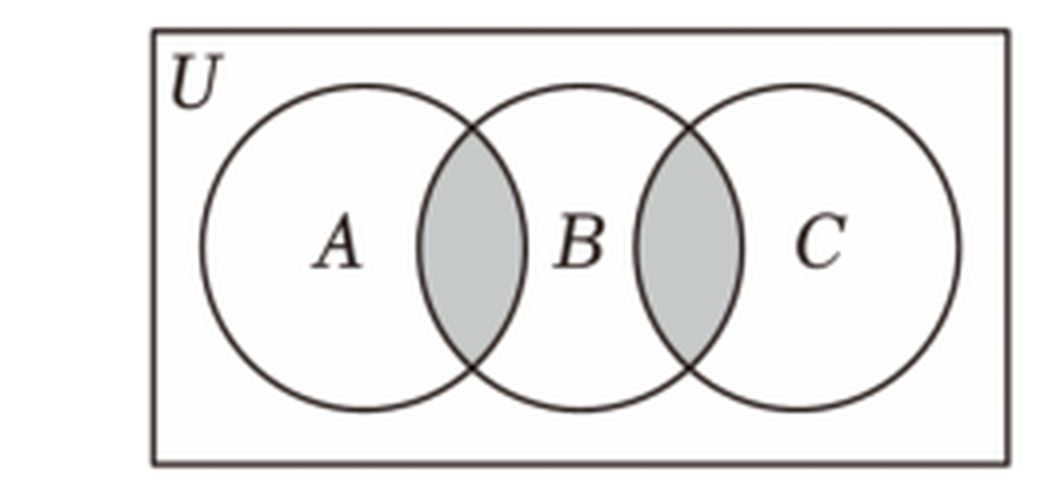
\includegraphics[width=0.30\textwidth]{figures/venn_ABC_lenses.png}
\end{center}

\keepwithprev
A. $B\cap(A\cup C)$\qquad\qquad\qquad B. $B\cap(A\cap C)$

C. $B\cap\complement_U(A\cup C)$\qquad\qquad D. $(A\cup B)\cap(B\cup C)$

\ans{$A$}

\ifanswer
\solbegin
\step{由图中阴影部分得，阴影为集合 $A$、$B$ 的交集和 $B$、$C$ 的交集的并集，}
\step{故阴影部分可表示为 $(A\cap B)\cup(B\cap C)$ 或 $B\cap(A\cup C)$，
故 $A$ 正确. 故选 $A$.}
\solend

\fi

\item 设集合 $P_1=\{x\mid x^2+ax+1>0\}$，$P_2=\{x\mid x^2+ax+2>0\}$，
$Q_1=\{x\mid x^2+x+b>0\}$，$Q_2=\{x\mid x^2+2x+b>0\}$，其中 $a$、$b\in\R$，
对于下列两个命题：①存在 $a$，$P_1$ 不是 $P_2$ 的子集；②存在 $b$ 使得 $Q_1$ 是 $Q_2$
的子集. 下列说法正确的是\mbox{（\quad）}

\keepwithprev
A. ①是真命题，②是假命题\qquad B. ①是假命题，②是真命题

C. ①②都是真命题\qquad\qquad\quad D. ①②都是假命题

\ans{$B$}

\ifanswer
\solbegin
\step{对于集合 $P_1=\{x\mid x^2+ax+1>0\}$，$P_2=\{x\mid x^2+ax+2>0\}$，}
\step{得当 $m\in P_1$ 时，即 $m^2+am+1>0$，得 $m^2+am+2>0$，}
\step{即有 $m\in P_2$，得对任意 $a$，$P_1$ 是 $P_2$ 的子集，故①错误；}
\step{对于集合 $Q_1=\{x\mid x^2+x+b>0\}$，$Q_2=\{x\mid x^2+2x+b>0\}$，}
\step{当 $b=6$ 时，$Q_1=\{x\mid x^2+x+6>0\}=\R$，$Q_2=\{x\mid x^2+2x+6>0\}=\R$，}
\step{得 $Q_1$ 是 $Q_2$ 的子集，所以存在 $b$，使得 $Q_1$ 是 $Q_2$ 的子集，故②正确；}
\step{故选 $B$.}
\solend

\fi

\item 设 $a$、$b\in\R$，则“$a+b>2$ 且 $ab>1$”是“$a>1$ 且 $b>1$”的\mbox{（\quad）}

\keepwithprev
A. 充要条件\qquad\qquad\qquad B. 充分不必要条件

C. 必要不充分条件\qquad\quad D. 既不充分又不必要条件

\ans{$C$}

\ifanswer
\solbegin
\step{因为 $a>1$ 且 $b>1$，所以 $a+b>2$ 且 $ab>1$，}
\step{若已知 $a+b>2$ 且 $ab>1$，可取 $a=\dfrac12$，$b=8$，也满足已知，}
\step{所以“$a+b>2$ 且 $ab>1$”是“$a>1$ 且 $b>1$”的必要不充分条件，故选 $C$.}
\solend

\fi

\item 十七世纪，数学家费马提出猜想：“对任意正整数 $n>2$，关于 $x$、$y$、$z$ 的方程
$x^n+y^n=z^n$ 没有正整数解”. 1995 年数学家安德鲁·怀尔斯发表了完成的证明过程，使它
终成费马大定理. 对费马大定理，若用反证法证明，第一步是假设猜想不成立，即\mbox{（\quad）}

\keepwithprev
A. 对任意正整数 $n>2$，关于 $x$、$y$、$z$ 的方程 $x^n+y^n=z^n$ 都有正整数解

B. 对任意正整数 $n>2$，关于 $x$、$y$、$z$ 的方程 $x^n+y^n=z^n$ 至少存在一组正整数解

C. 存在正整数 $n\leqslant2$，关于 $x$、$y$、$z$ 的方程 $x^n+y^n=z^n$ 至少存在一组正整数解

D. 存在正整数 $n>2$，关于 $x$、$y$、$z$ 的方程 $x^n+y^n=z^n$ 至少存在一组正整数解

\ans{$D$}

\end{enumerate}

\bigsec{三、解答题}

\begin{enumerate}
\setcounter{enumi}{16}

\item 已知 $a$、$b$、$c$ 都是实数，且 $a+b+c=0$，$abc=1$，求证：$a$、$b$、$c$ 中必有一个
大于 $\dfrac32$.

\ifanswer
\solbegin
\step{由 $a+b+c=0$，$abc=1$，得 $a$、$b$、$c$ 中一个正数，两个负数，}
\step{不妨设 $c>0$，由题意得 $a+b=-c,ab=\dfrac1c$，}
\step{由根与系数的关系得 $a$、$b$ 是关于 $x$ 的方程 $x^2+cx+\dfrac1c=0$ 的两个根，}
\step{则 $\Delta=c^2-\dfrac4c=\dfrac{c^3-4}{c}\geqslant0$，}
\step{因为 $c>0$，所以 $c^3\geqslant4$，得 $c\geqslant\sqrt[3]{4}$，}
\step{又 $\dfrac32=\sqrt[3]{\left(\dfrac32\right)^3}=\sqrt[3]{\dfrac{27}{8}}<\sqrt[3]{4}$，}
\step{所以 $c>\dfrac32$，即 $a$、$b$、$c$ 中必有一个大于 $\dfrac32$.}
\solend

\fi

\ansspace[6]

\item 已知关于 $x$ 的一元二次方程 $x^2-mx+4m^2-3=0$ 的两个实根分别为 $x_1,x_2$.

\begin{enumerate}[label=(\arabic*)]
\item $x_1,x_2$ 均为正根，求实数 $m$ 的取值范围；
\item 若 $x_1,x_2$ 满足：$x_1+x_2=x_1x_2$，求实数 $m$ 的值.
\end{enumerate}

\ifanswer
\solbegin
\stepm{(1)}{由 $x_1,x_2$ 均为正根，得}
\step{$\begin{cases}\Delta=(-m)^2-4(4m^2-3)\geqslant0\\ x_1+x_2=m>0\\ x_1\cdot x_2=4m^2-3>0\end{cases}$，}
\step{解得 $\begin{cases}-\dfrac{2\sqrt5}{5}\leqslant m\leqslant\dfrac{2\sqrt5}{5}\\[4pt]
m>0\\[4pt] m\leqslant-\dfrac{\sqrt3}{2}$ 或 $m\geqslant\dfrac{\sqrt3}{2}\end{cases}$，}
\step{即 $\dfrac{\sqrt3}{2}\leqslant m\leqslant\dfrac{2\sqrt5}{5}$；}
\stepm{(2)}{由 (1) 得
$\begin{cases}-\dfrac{2\sqrt5}{5}\leqslant m\leqslant\dfrac{2\sqrt5}{5}\\[4pt]
m=4m^2-3\end{cases}$，解得 $m=1$（舍去）或 $m=-\dfrac34$，}
\step{则 $m=-\dfrac34$.}
\solend

\fi

\ansspace[6]

\item 已知集合 $A=\{x\mid m-1<x<m^2+1\}$，$B=\{x\mid-2<x<2\}$.

\begin{enumerate}[label=(\arabic*)]
\item 当 $m=2$ 时，求 $A\cup B$、$A\cap B$、$\complement_R B$、$A\cap(\complement_R B)$；
\item 若“$x\in A$”是“$x\in B$”成立的必要不充分条件，求实数 $m$ 的取值范围.
\end{enumerate}

\ifanswer
\solbegin
\stepm{(1)}{$m=2$ 时，$A=\{x\mid1<x<5\}$，且 $B=\{x\mid-2<x<2\}$，}
\step{所以 $A\cup B=\{x\mid-2<x<5\}$，$A\cap B=\{x\mid1<x<2\}$，}
\step{$\complement_R B=\{x\mid x\leqslant-2$ 或 $x\geqslant2\}$，
$A\cap(\complement_R B)=\{x\mid2\leqslant x<5\}$；}
\stepm{(2)}{若“$x\in A$”是“$x\in B$”成立的必要不充分条件，则 $B\subset A$，}
\step{所以 $\begin{cases}m-1<-2\\ m^2+1\geqslant2\end{cases}$
或 $\begin{cases}m-1\leqslant-2\\ m^2+1>2\end{cases}$，解得 $m<-1$，}
\step{故 $m$ 的取值范围为 $(-\infty,-1)$.}
\solend

\fi

\ansspace[6]

\item 已知 $m\in\R$，集合 $A=\{x\mid|x-1|\leqslant2\}$，集合
$B=\{x\mid m-3<x\leqslant m+2\}$.

\begin{enumerate}[label=(\arabic*)]
\item 若“$x\in A$”是“$x\in B$”的充分不必要条件，求 $m$ 的取值范围；
\item 若命题“$\forall x\in B$，$x\in\complement_R A$”是真命题，求 $m$ 的取值范围；
\item 若命题“$\exists x\in A$，$x\in B$”是真命题，求 $m$ 的取值范围.
\end{enumerate}

\ifanswer
\solbegin
\stepm{(1)}{集合 $A=\{x\mid|x-1|\leqslant2\}=\{x\mid-1\leqslant x\leqslant3\}$，}
\step{若“$x\in A$”是“$x\in B$”的充分不必要条件，则 $A\subset B$，}
\step{所以 $\begin{cases}m-3<-1\\ 3\leqslant m+2\end{cases}$，解得 $1\leqslant m<2$，}
\step{当 $m=1$ 时，$B=\{x\mid-2<x\leqslant3\}$，符合题意，}
\step{所以 $m$ 的取值范围是 $\{m\mid1\leqslant m<2\}$.}
\stepm{(2)}{若命题“$\forall x\in B$，$x\in\complement_R A$”是真命题，则 $B\subset\complement_R A$，}
\step{又 $\complement_R A=\{x\mid x<-1$ 或 $x>3\}$，$B\neq\varnothing$，
所以 $m+2<-1$ 或 $m-3\geqslant3$，}
\step{解得 $m<-3$ 或 $m\geqslant6$，所以 $\{m\mid m<-3$ 或 $m\geqslant6\}$；}
\stepm{(3)}{因为 $\exists x\in A$，$x\in B$ 是真命题，所以 $A\cap B\neq\varnothing$，}
\step{当 $A\cap B=\varnothing$ 时，所以 $m+2<-1$ 或 $m-3\geqslant3$，
即 $m<-3$ 或 $m\geqslant6$，}
\step{所以当 $A\cap B\neq\varnothing$ 时，$m$ 的取值范围是 $\{m\mid-3\leqslant m<6\}$，}
\step{则 $m$ 的取值范围是 $\{m\mid-3\leqslant m<6\}$.}
\solend

\fi

\ansspace[6]

\item 对于函数 $f(x)$，若 $f(x_0)=x_0$，则称 $x_0$ 为 $f(x)$ 的“不动点”；若
$f[f(x_0)]=x_0$，则称 $x_0$ 为 $f(x)$ 的“稳定点”. 函数 $f(x)$ 的“不动点”和“稳定点”
的集合分别记为 $A$ 和 $B$，即 $A=\{x\mid f(x)=x\}$，$B=\{x\mid f[f(x)]=x\}$.

\begin{enumerate}[label=(\arabic*)]
\item 设函数 $f(x)=3x+4$，求集合 $A$ 和 $B$；
\item 求证：$A\sub B$；
\item 设函数 $f(x)=ax^2+bx+c(a\neq0)$，且 $A=\varnothing$，求证：$B=\varnothing$.
\end{enumerate}

\ifanswer
\solbegin
\stepm{(1)}{令 $f(x)=3x+4=x$，解得 $x=-2$，故有 $A=\{-2\}$，}
\step{由于 $f[f(x)]=3(3x+4)+4=9x+16$，}
\step{令 $9x+16=x$，得 $x=-2$，故有 $B=\{-2\}$；}
\stepm{(2)}{若 $A=\varnothing$，则 $A\sub B$ 显然成立；}
\step{若 $A\neq\varnothing$，设 $t\in A$，则 $f(t)=t$，$f(f(t))=f(t)=t$，}
\step{所以 $t\in B$，故 $A\sub B$.}
\stepm{(3)}{因为 $A=\{x\mid f(x)=x\}=\varnothing$，所以 $ax^2+bx+c=x$ 无解，}
\step{即 $\Delta=(b-1)^2-4a<0$，}
\step{①当 $a>0$ 时，二次函数 $y=f(x)-x$，}
\step{即 $y=ax^2+(b-1)x+c$ 的图象在 $x$ 轴的上方，}
\step{所以 $\forall x\in\R$，$f(x)-x>0$ 恒成立，所以 $\forall x\in\R$，
$f(x)>x$ 恒成立，}
\step{所以 $\forall x\in\R$，$f[f(x)]>f(x)>x$ 恒成立，即 $B=\varnothing$；}
\step{②当 $a<0$ 时，同理可证 $B=\varnothing$；}
\step{综上，对于函数 $f(x)=ax^2+bx+c(a\neq0)$，当 $A=\varnothing$ 时，$B=\varnothing$.}
\solend

\fi

\ansspace*[10]

\end{enumerate}

\end{document}
"
% 紧凑版：xelatex "\def\iscompact{1}% 高一26_交附闵行_周练2.tex
%   —— 高一上数学「2026-2027 年交附闵行高一上周练 2」（试卷版/答案版）
% 试卷版：xelatex 高一26_交附闵行_周练2.tex
% 答案版：xelatex "\def\isanswer{1}\input{高一26_交附闵行_周练2.tex}"
% 紧凑版：xelatex "\def\iscompact{1}\input{高一26_交附闵行_周练2.tex}"
%
% 原始材料是微信公众号图文（公众号「魔都数学加油站」连载「27学年高一 26」，2026-09-21 发布，
% 原文标题「27学年高一26——2026-2027年上海市交附闵行高一上周练2」），
% 正文为 10 张 PNG 页（1080×1527，各页同尺寸）。原文本身就是一份**讲评版**——
% 题目下方直接印出【解析】（本卷无单独的【答案】行，填空题答案都写在解析里）。
% 试题文字与解析均照原卷录入，未改内容。卷面的粉色斜水印「魔都数学加油站」属水印，未录入。
%
% 卷首标题：原卷印作「2026-2027 年交附闵行高一上周练 2」（公众号标题里的「上海市」
% 三字卷面标题行没有，本稿照卷面），年份区间按全稿惯例排 en dash，前缀照原卷保留「年」。
%
% 与原卷的排版差异（均已在 README「说明」中交代）：
%   ① 原文自**第 3 题**起（第 1、2 题未在该文中发布），故本稿题号亦自 3 起；
%   ② 原卷本就印有「一、填空题」「二、选择题」「三、解答题」三节标题，本稿照原卷分节，
%      只把标题改排成全稿统一的「大节标题」样式；
%   ③ 原卷第 16 题的答案「D」直接印在题干末尾的括号内（原卷把括号连同 D 单独占一行），
%      第 13—15 题的括号空着、答案写在解析末句「故选 A／B／C」里；填空题的答案也都嵌在
%      解析里，本稿统一改为试卷版隐去、答案版以 \ans{} 给出（选择题另附【解析】）；
%   ④ 子集符号原卷两种并用：第 4 题题干与第 8 题、第 21(2) 题等作带下划线的 $\subseteq$，
%      第 19(2)、20(1)(2) 题作真包含的 $\subset$，本稿分别照录为 $\sub$ 与 $\subset$；
%   ⑤ 补集符号原卷作 $\complement_R$、$\complement_U$（第 4 题命题④、第 13 题选项 C、
%      第 19—20 题），本稿照录；
%   ⑥ 原卷的实数集 R 一律作斜体（第 11 题「$a\in R$」、第 14 题「$a$、$b\in R$」与解析的
%      $\{x\mid x^2+x+6>0\}=R$ 等），本稿按全稿惯例统一写作 $\R$；
%   ⑦ 原卷填空的横线约两个字宽，本稿按全稿惯例统一排 \blankline[4.4em]；
%   ⑧ 原卷未印副标题，本稿按全稿惯例补出副标题「集合与常用逻辑用语」；
%   ⑨ 第 13 题的 Venn 图原卷印在题干右侧（第 5 页），本稿移至题干之后；
%      图取原卷截图、4× LANCZOS 放大（figures/venn_ABC_lenses.png，
%      阴影为 $A\cap B$ 与 $B\cap C$ 两个交带，即 $(A\cap B)\cup(B\cap C)$）。
%
% 原卷存疑一处（照抄原卷、未改，见源码中该处上方注释）：
%   ① 第 12 题【解析】首步的方程组里印 $t<2$，而其后三处与末行答案都作 $t\leqslant2$
%      （$\left[\dfrac85,\dfrac{17}{10}\right)\cup\left(\dfrac95,2\right]$ 含 $2$）——
%      按题意 $N=\left\{x\mid t-\dfrac35\leqslant x\leqslant t\right\}\sub\{x\mid1\leqslant x\leqslant2\}$
%      只要求 $t\leqslant2$（$t=2$ 时 $N=\left[\dfrac75,2\right]$ 确实含于其中），
%      故方程组里的 $t<2$ 应是原卷笔误；本稿两处都照原卷录入、未互相迁就。
% 另：第 20(3) 题解析末两行原卷即作同话重复，照原卷录入。

\documentclass[a4paper,11pt]{article}
\usepackage{common}

\begin{document}

\examtitlest[3]{2026--2027 年交附闵行高一上周练 2}{集合与常用逻辑用语}

\bigsec{一、填空题}

\begin{enumerate}
\setcounter{enumi}{2}

\item 命题甲：集合 $M=\{x\mid kx^2-2kx+1=0\}$ 为空集；命题乙：关于 $x$ 的不等式
$x^2+(k-1)x+4>0$ 的解集为 $\R$. 若命题甲、乙中有且只有一个是真命题，则实数 $k$ 的取
值范围是 \blankline[4.4em].

\ifanswer
\solbegin
\step{因为集合 $M=\{x\mid kx^2-2kx+1=0\}$ 为空集，}
\step{当 $k\neq0$ 时，$\Delta=(-2k)^2-4k<0$，解得 $0<k<1$，}
\step{当 $k=0$ 时，方程变为 $1=0$，无解，满足题意，故 $0\leqslant k<1$；}
\step{又关于 $x$ 的不等式 $x^2+(k-1)x+4>0$ 的解集为 $\R$，}
\step{所以 $\Delta'=(k-1)^2-4\times4<0$，解得 $-3<k<5$，}
\step{当甲命题为真，乙命题为假时，无解，}
\step{当甲命题为假，乙命题为真时，$k\in(-3,0)\cup[1,5)$.}
\solend

\fi

\item 对任意 $A$、$B\sub\R$，记 $A\oplus B=\{x\mid x\in A\cup B,x\notin A\cap B\}$，
并称 $A\oplus B$ 为集合 $A$、$B$ 的对称差. 例如：若 $A=\{1,2,3\},B=\{2,3,4\}$，
则 $A\oplus B=\{1,4\}$. 下列命题中，为真命题的是 \blankline[4.4em].

\keepwithprev
①若 $A$、$B\sub\R$ 且 $A\oplus B\sub A$，则 $A\sub B$

②若 $A$、$B\sub\R$ 且 $A\oplus B=\varnothing$，则 $A=B$

③若 $A$、$B\sub\R$ 且 $A\oplus B=B$，则 $A=\varnothing$

④对任意 $A$、$B\sub\R$，都有 $A\oplus B=\complement_R A\oplus\complement_R B$

\ans{②③④}

\ifanswer
\solbegin
\step{对于①，因为 $A\oplus B\sub A$，
所以 $\{x\mid x\in A\cup B,x\notin A\cap B\}\sub A$，}
\step{故 $B\sub A$，①错误；}
\step{对于②，$A$、$B\sub\R$ 且 $A\oplus B=\varnothing$，
则 $\varnothing=\{x\mid x\in A\cup B,x\notin A\cap B\}$，}
\step{即 $A\cup B=A\cap B$，所以 $A=B$，②正确；}
\step{对于③，$A$、$B\sub\R$ 且 $A\oplus B=B$，
则 $B=\{x\mid x\in A\cup B,x\notin A\cap B\}$，}
\step{故 $A\sub B$，且 $B$ 中元素不在 $A\cap B$ 中，故 $A=\varnothing$，③正确；}
\step{对于④，$\complement_R A\oplus\complement_R B
=\{x\mid x\in\complement_R A\cup\complement_R B,x\notin\complement_R A\cap\complement_R B\}$，}
\step{其中 $\complement_R A\cup\complement_R B=\complement_R(A\cap B)$，
$\complement_R A\cap\complement_R B=\complement_R(A\cup B)$，}
\step{故 $\complement_R A\oplus\complement_R B
=\{x\mid x\in\complement_R(A\cap B),x\notin\complement_R(A\cup B)\}
=\{x\mid x\in A\cup B,x\notin A\cap B\}$，}
\step{而 $A\oplus B=\{x\mid x\in A\cup B,x\notin A\cap B\}$，
故 $A\oplus B=\complement_R A\oplus\complement_R B$，④正确.}
\step{故正确的是②③④.}
\solend

\fi

\item 已知 $A=\{a_1,a_2,a_3,a_4\},B=\{a^2\mid a\in A\}$，其中 $a_1<a_2<a_3<a_4$，
且 $a_1$、$a_2$、$a_3$、$a_4$ 均为整数，若 $A\cap B=\{a_3,a_4\},a_1+a_3=0$，
且 $A\cup B$ 中的所有元素之和为 $270$，则集合 $A$ 中所有元素之和为 \blankline[4.4em].

\ifanswer
\solbegin
\step{$A=\{a_1,a_2,a_3,a_4\},B=\{a^2\mid a\in A\}$，
因为 $A\cap B=\{a_3,a_4\},a_1+a_3=0$，}
\step{所以 $A=\{a_1,a_2,a_3,a_4\},B=\left\{a_1^2,a_2^2,a_4^2\right\}$，}
\step{若 $a_1^2=a_3$，则 $a_1=-1,a_3=1$，则 $a_2=0$，
此时 $A=\{-1,0,1,a_4\},B=\{0,1,a_4^2\}$，}
\step{因为 $A\cup B$ 中的所有元素之和为 $270$，
所以 $-1+0+1+a_4+1+a_4^2=270$，}
\step{无正整数解，舍去；}
\step{若 $a_2^2=a_3$，① $a_4^2=a_4$，所以 $a_4=1$，矛盾；}
\step{② $a_1^2=a_4$，此时 $A\cup B=\left\{-a_2^2,a_2,a_2^2,a_1^2,a_4^2\right\}$，
所以 $a_2^8+a_2^4+a_2=270$，}
\step{所以 $a_2=-2$，此时 $a_1=-4,a_2=-2,a_3=4,a_4=16$；}
\step{若 $a_4^2=a_3$，显然不成立；}
\step{综上，集合 $A$ 中所有元素之和为 $-4-2+4+16=14$.}
\solend

\fi

\item 将集合 $M=\{a_1,a_2,a_3,\cdots,a_n\}$ 分拆成两个集合 $A_i$ 和 $B_j$，且
$M\supseteq A_i\cup B_j$，$A_i\cap B_j=\varnothing$，这样的分拆方法共有 \blankline[4.4em] 种.

\ifanswer
\solbegin
\step{按集合 $A_i$ 中的元素个数进行分类：}
\step{若 $A_i$ 中有 $0$ 个元素（即 $C_n^0$ 种）时，则 $B_j$ 有 $2^n$ 种，
共有 $2^nC_n^0$ 种；}
\step{若 $A_i$ 中有 $1$ 个元素（即 $C_n^1$ 种）时，则 $B_j$ 有 $2^{n-1}$ 种，
共有 $2^{n-1}C_n^1$ 种；}
\step{若 $A_i$ 中有 $2$ 个元素（即 $C_n^2$ 种）时，则 $B_j$ 有 $2^{n-2}$ 种，
共有 $2^{n-2}C_n^2$ 种；}
\step{若 $A_i$ 中有 $3$ 个元素（即 $C_n^3$ 种）时，则 $B_j$ 有 $2^{n-3}$ 种，
共有 $2^{n-3}C_n^3$ 种；}
\step{若 $A_i$ 中有 $n$ 个元素（即 $C_n^n$ 种）时，则 $B_j$ 有 $2^0$ 种，
共有 $2^0C_n^n$ 种；}
\step{得 $2^nC_n^0+2^{n-1}C_n^1+2^{n-2}C_n^2+\cdots+2^0C_n^n=(1+2)^n$，
故这样的分拆方法有 $3^n$ 种.}
\solend

\fi

\item 已知集合 $A=\{x\mid x<2,x\in\Z\}$，$B=\{x\mid x>0,x\in\Z\}$，则
$A\cap B=$ \blankline[4.4em].

\ifanswer
\solbegin
\step{因为 $A=\{x\mid x<2,x\in\Z\}$，$B=\{x\mid x>0,x\in\Z\}$，}
\step{所以 $A\cap B=\{x\mid0<x<2,x\in\Z\}=\{1\}$.}
\solend

\fi

\item 已知集合 $A=\{x\mid(a-1)x^2+3x-2=0\}$，$B=\{x\mid x^2-3x+2=0\}$，若
$A\sub B$，求实数 $a$ 的取值范围是 \blankline[4.4em].

\ifanswer
\solbegin
\step{由方程 $x^2-3x+2=0$，解得 $x=1$ 或 $x=2$，即 $B=\{1,2\}$，}
\step{因为 $A\sub B$，所以 $A=\varnothing$ 或 $A=\{1\}$ 或 $A=\{2\}$ 或 $A=\{1,2\}$，}
\step{当 $A=\varnothing$ 时，
则 $\begin{cases}a\neq1\\ \Delta=3^2-4(a-1)\times(-2)<0\end{cases}$，
解得 $a<-\dfrac18$；}
\step{将 $x=1$ 代入方程 $(a-1)x^2+3x-2=0$，得 $a=0$，}
\step{此时 $A=\{x\mid-x^2+3x-2=0\}=\{1,2\}$，满足条件；}
\step{将 $x=2$ 代入方程 $(a-1)x^2+3x-2=0$，得到 $a=0$，上面已经验证满足条件；}
\step{综上所述，$a$ 的取值范围是 $\left(-\infty,-\dfrac18\right)\cup\{0\}$.}
\solend

\fi

\item 已知方程 $x^2-3x+a=0$ 的两根都大于 $1$，则 $a$ 的取值范围为 \blankline[4.4em].

\ifanswer
\solbegin
\step{由题意得 $\Delta=9-4a\geqslant0$，$x_1+x_2=3$，$x_1x_2=a$，
所以 $a\leqslant\dfrac94$，}
\step{则 $(x_1-1)(x_2-1)=x_1x_2-(x_1+x_2)+1=a-3+1>0$，所以 $a>2$，}
\step{故 $a$ 的范围为 $\left(2,\dfrac94\right]$.}
\solend

\fi

\item 设 $x_1$、$x_2$ 是方程 $x^2+x-3=0$ 的两个实数根，则 $x_1^2-x_2+2024=$
\blankline[4.4em].

\ifanswer
\solbegin
\step{由题意得 $x_1^2=3-x_1$，$x_1+x_2=-1$，}
\step{则 $x_1^2-x_2+2024=3-x_1-x_2+2024=2027-(-1)=2028$.}
\solend

\fi

\item 已知 $a\in\R$，若关于 $x$ 的方程 $x^2+ax+a^2-8=0$ 有两个实根 $x_1$、$x_2$，且
$\dfrac1{x_1}+\dfrac1{x_2}=-\dfrac12$，则 $a$ 的值为 \blankline[4.4em].

\ifanswer
\solbegin
\step{由题意得 $\Delta=a^2-4(a^2-8)=32-3a^2\geqslant0$，
解得 $a^2\leqslant\dfrac{32}{3}$，}
\step{由韦达定理得 $x_1+x_2=-a$，$x_1x_2=a^2-8$，}
\step{则 $\dfrac1{x_1}+\dfrac1{x_2}=\dfrac{x_1+x_2}{x_1x_2}
=\dfrac{-a}{a^2-8}=-\dfrac12$，}
\step{即 $a^2-2a-8=(a-4)(a+2)=0$，解得 $a=4$ 或 $a=-2$.}
\step{又 $a^2\leqslant\dfrac{32}{3}$，则 $a=-2$.}
\solend

\fi

\item 定义集合 $P=\{x\mid a\leqslant x\leqslant b\}$ 的“长度”是 $b-a$，其中 $a$、
$b\in\R$. 已知集合 $M=\left\{x\mid\dfrac65\leqslant x\leqslant\dfrac{17}{10}\right\}$，
$N=\left\{x\mid t-\dfrac35\leqslant x\leqslant t\right\}$，且 $M$、$N$ 都是集合
$\{x\mid1\leqslant x\leqslant2\}$ 的子集，若集合 $M\cup N$ 的“长度”大于 $\dfrac35$，
则 $t$ 的取值范围是 \blankline[4.4em].

\ifanswer
\solbegin
\step{因为 $N=\left\{x\mid t-\dfrac35\leqslant x\leqslant t\right\}$
是集合 $\{x\mid1\leqslant x\leqslant2\}$ 的子集，}
% 注：下一行方程组里的 $t<2$ 系原卷所印（本稿照录），与其后三处及末行答案的
%     $t\leqslant2$ 自相矛盾——按题意应为 $t\leqslant2$，见文件头「原卷存疑」①。
\step{所以 $\begin{cases}t-\dfrac35\geqslant1\\[2pt] t<2\end{cases}$，
解得 $\dfrac85\leqslant t\leqslant2$，}
\step{又 $M=\left\{x\mid\dfrac65\leqslant x\leqslant\dfrac{17}{10}\right\}$，
得集合 $M$ 的“长度”为 $\dfrac{17}{10}-\dfrac65=\dfrac12$，}
\step{又 $N=\left\{x\mid t-\dfrac35\leqslant x\leqslant t\right\}$，
要使集合 $M\cup N$ 的“长度”大于 $\dfrac35$，}
\step{若 $M\cup N=\left\{x\mid t-\dfrac35\leqslant x\leqslant\dfrac{17}{10}\right\}$，
则 $\dfrac{17}{10}-t+\dfrac35>\dfrac35$，所以 $t<\dfrac{17}{10}$，}
\step{又 $\dfrac85\leqslant t\leqslant2$，所以 $\dfrac85\leqslant t<\dfrac{17}{10}$；}
\step{若 $M\cup N=\left\{x\mid\dfrac65\leqslant x\leqslant t\right\}$，
则 $t-\dfrac65>\dfrac35$，所以 $t>\dfrac95$，}
\step{又 $\dfrac85\leqslant t\leqslant2$，所以 $\dfrac95<t\leqslant2$；}
\step{则 $t$ 的取值范围是 $\left[\dfrac85,\dfrac{17}{10}\right)\cup\left(\dfrac95,2\right]$.}
\solend

\fi

\end{enumerate}

% 第 13 题是「题干 + 图 + 选项」约 5.7cm 的一整块（图 0.30\textwidth、宽高比 0.477 → 高 2.29cm，
% 加题干 1 行、选项 2 行与段间距）。`\keepwithprev` 只挡得住「题干—选项」之间，挡不住
% 夹在中间的图——实测断点落在题干之后，题干孤零零留在 p1、图与四个选项整页翻到 p2
% （切页审计的 A 类）。故照 高一30 第 4 题的成例先量一次页高；**守卫要放在 `\bigsec` 之前**
% 连节标题一起量（放标题之后会把「二、选择题」孤立在页末，正是 高一40 修过的那类 B 类）。
% 7cm ＝ 节标题约 1.1cm ＋ 第 13 题那块约 5.7cm（留少量余量）。
\needvspace{7cm}
\bigsec{二、选择题}

\begin{enumerate}
\setcounter{enumi}{12}

\item 图中阴影部分用集合符号可以表示为\mbox{（\quad）}

\begin{center}
% 图取原卷截图、4× LANCZOS 放大（原卷把图印在题干右侧，本稿移至此处，见文件头⑨）。
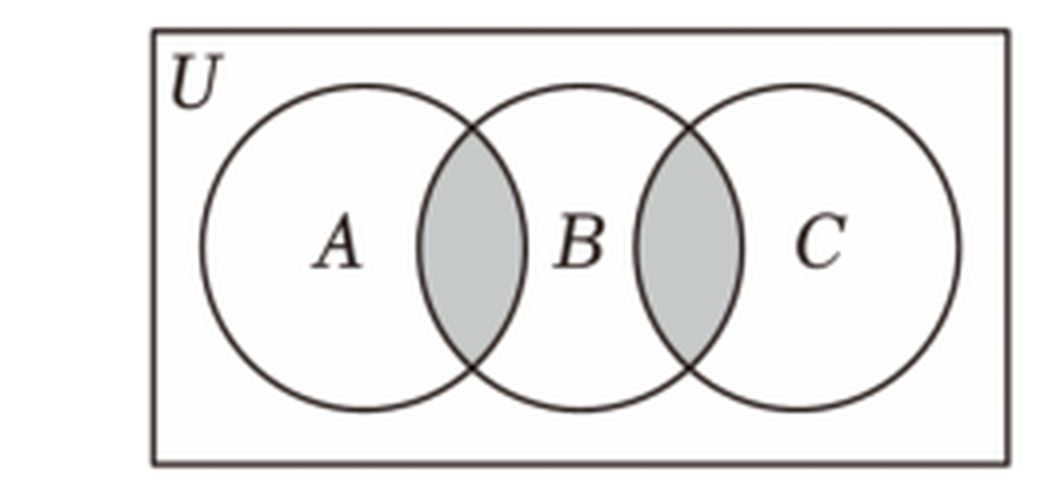
\includegraphics[width=0.30\textwidth]{figures/venn_ABC_lenses.png}
\end{center}

\keepwithprev
A. $B\cap(A\cup C)$\qquad\qquad\qquad B. $B\cap(A\cap C)$

C. $B\cap\complement_U(A\cup C)$\qquad\qquad D. $(A\cup B)\cap(B\cup C)$

\ans{$A$}

\ifanswer
\solbegin
\step{由图中阴影部分得，阴影为集合 $A$、$B$ 的交集和 $B$、$C$ 的交集的并集，}
\step{故阴影部分可表示为 $(A\cap B)\cup(B\cap C)$ 或 $B\cap(A\cup C)$，
故 $A$ 正确. 故选 $A$.}
\solend

\fi

\item 设集合 $P_1=\{x\mid x^2+ax+1>0\}$，$P_2=\{x\mid x^2+ax+2>0\}$，
$Q_1=\{x\mid x^2+x+b>0\}$，$Q_2=\{x\mid x^2+2x+b>0\}$，其中 $a$、$b\in\R$，
对于下列两个命题：①存在 $a$，$P_1$ 不是 $P_2$ 的子集；②存在 $b$ 使得 $Q_1$ 是 $Q_2$
的子集. 下列说法正确的是\mbox{（\quad）}

\keepwithprev
A. ①是真命题，②是假命题\qquad B. ①是假命题，②是真命题

C. ①②都是真命题\qquad\qquad\quad D. ①②都是假命题

\ans{$B$}

\ifanswer
\solbegin
\step{对于集合 $P_1=\{x\mid x^2+ax+1>0\}$，$P_2=\{x\mid x^2+ax+2>0\}$，}
\step{得当 $m\in P_1$ 时，即 $m^2+am+1>0$，得 $m^2+am+2>0$，}
\step{即有 $m\in P_2$，得对任意 $a$，$P_1$ 是 $P_2$ 的子集，故①错误；}
\step{对于集合 $Q_1=\{x\mid x^2+x+b>0\}$，$Q_2=\{x\mid x^2+2x+b>0\}$，}
\step{当 $b=6$ 时，$Q_1=\{x\mid x^2+x+6>0\}=\R$，$Q_2=\{x\mid x^2+2x+6>0\}=\R$，}
\step{得 $Q_1$ 是 $Q_2$ 的子集，所以存在 $b$，使得 $Q_1$ 是 $Q_2$ 的子集，故②正确；}
\step{故选 $B$.}
\solend

\fi

\item 设 $a$、$b\in\R$，则“$a+b>2$ 且 $ab>1$”是“$a>1$ 且 $b>1$”的\mbox{（\quad）}

\keepwithprev
A. 充要条件\qquad\qquad\qquad B. 充分不必要条件

C. 必要不充分条件\qquad\quad D. 既不充分又不必要条件

\ans{$C$}

\ifanswer
\solbegin
\step{因为 $a>1$ 且 $b>1$，所以 $a+b>2$ 且 $ab>1$，}
\step{若已知 $a+b>2$ 且 $ab>1$，可取 $a=\dfrac12$，$b=8$，也满足已知，}
\step{所以“$a+b>2$ 且 $ab>1$”是“$a>1$ 且 $b>1$”的必要不充分条件，故选 $C$.}
\solend

\fi

\item 十七世纪，数学家费马提出猜想：“对任意正整数 $n>2$，关于 $x$、$y$、$z$ 的方程
$x^n+y^n=z^n$ 没有正整数解”. 1995 年数学家安德鲁·怀尔斯发表了完成的证明过程，使它
终成费马大定理. 对费马大定理，若用反证法证明，第一步是假设猜想不成立，即\mbox{（\quad）}

\keepwithprev
A. 对任意正整数 $n>2$，关于 $x$、$y$、$z$ 的方程 $x^n+y^n=z^n$ 都有正整数解

B. 对任意正整数 $n>2$，关于 $x$、$y$、$z$ 的方程 $x^n+y^n=z^n$ 至少存在一组正整数解

C. 存在正整数 $n\leqslant2$，关于 $x$、$y$、$z$ 的方程 $x^n+y^n=z^n$ 至少存在一组正整数解

D. 存在正整数 $n>2$，关于 $x$、$y$、$z$ 的方程 $x^n+y^n=z^n$ 至少存在一组正整数解

\ans{$D$}

\end{enumerate}

\bigsec{三、解答题}

\begin{enumerate}
\setcounter{enumi}{16}

\item 已知 $a$、$b$、$c$ 都是实数，且 $a+b+c=0$，$abc=1$，求证：$a$、$b$、$c$ 中必有一个
大于 $\dfrac32$.

\ifanswer
\solbegin
\step{由 $a+b+c=0$，$abc=1$，得 $a$、$b$、$c$ 中一个正数，两个负数，}
\step{不妨设 $c>0$，由题意得 $a+b=-c,ab=\dfrac1c$，}
\step{由根与系数的关系得 $a$、$b$ 是关于 $x$ 的方程 $x^2+cx+\dfrac1c=0$ 的两个根，}
\step{则 $\Delta=c^2-\dfrac4c=\dfrac{c^3-4}{c}\geqslant0$，}
\step{因为 $c>0$，所以 $c^3\geqslant4$，得 $c\geqslant\sqrt[3]{4}$，}
\step{又 $\dfrac32=\sqrt[3]{\left(\dfrac32\right)^3}=\sqrt[3]{\dfrac{27}{8}}<\sqrt[3]{4}$，}
\step{所以 $c>\dfrac32$，即 $a$、$b$、$c$ 中必有一个大于 $\dfrac32$.}
\solend

\fi

\ansspace[6]

\item 已知关于 $x$ 的一元二次方程 $x^2-mx+4m^2-3=0$ 的两个实根分别为 $x_1,x_2$.

\begin{enumerate}[label=(\arabic*)]
\item $x_1,x_2$ 均为正根，求实数 $m$ 的取值范围；
\item 若 $x_1,x_2$ 满足：$x_1+x_2=x_1x_2$，求实数 $m$ 的值.
\end{enumerate}

\ifanswer
\solbegin
\stepm{(1)}{由 $x_1,x_2$ 均为正根，得}
\step{$\begin{cases}\Delta=(-m)^2-4(4m^2-3)\geqslant0\\ x_1+x_2=m>0\\ x_1\cdot x_2=4m^2-3>0\end{cases}$，}
\step{解得 $\begin{cases}-\dfrac{2\sqrt5}{5}\leqslant m\leqslant\dfrac{2\sqrt5}{5}\\[4pt]
m>0\\[4pt] m\leqslant-\dfrac{\sqrt3}{2}$ 或 $m\geqslant\dfrac{\sqrt3}{2}\end{cases}$，}
\step{即 $\dfrac{\sqrt3}{2}\leqslant m\leqslant\dfrac{2\sqrt5}{5}$；}
\stepm{(2)}{由 (1) 得
$\begin{cases}-\dfrac{2\sqrt5}{5}\leqslant m\leqslant\dfrac{2\sqrt5}{5}\\[4pt]
m=4m^2-3\end{cases}$，解得 $m=1$（舍去）或 $m=-\dfrac34$，}
\step{则 $m=-\dfrac34$.}
\solend

\fi

\ansspace[6]

\item 已知集合 $A=\{x\mid m-1<x<m^2+1\}$，$B=\{x\mid-2<x<2\}$.

\begin{enumerate}[label=(\arabic*)]
\item 当 $m=2$ 时，求 $A\cup B$、$A\cap B$、$\complement_R B$、$A\cap(\complement_R B)$；
\item 若“$x\in A$”是“$x\in B$”成立的必要不充分条件，求实数 $m$ 的取值范围.
\end{enumerate}

\ifanswer
\solbegin
\stepm{(1)}{$m=2$ 时，$A=\{x\mid1<x<5\}$，且 $B=\{x\mid-2<x<2\}$，}
\step{所以 $A\cup B=\{x\mid-2<x<5\}$，$A\cap B=\{x\mid1<x<2\}$，}
\step{$\complement_R B=\{x\mid x\leqslant-2$ 或 $x\geqslant2\}$，
$A\cap(\complement_R B)=\{x\mid2\leqslant x<5\}$；}
\stepm{(2)}{若“$x\in A$”是“$x\in B$”成立的必要不充分条件，则 $B\subset A$，}
\step{所以 $\begin{cases}m-1<-2\\ m^2+1\geqslant2\end{cases}$
或 $\begin{cases}m-1\leqslant-2\\ m^2+1>2\end{cases}$，解得 $m<-1$，}
\step{故 $m$ 的取值范围为 $(-\infty,-1)$.}
\solend

\fi

\ansspace[6]

\item 已知 $m\in\R$，集合 $A=\{x\mid|x-1|\leqslant2\}$，集合
$B=\{x\mid m-3<x\leqslant m+2\}$.

\begin{enumerate}[label=(\arabic*)]
\item 若“$x\in A$”是“$x\in B$”的充分不必要条件，求 $m$ 的取值范围；
\item 若命题“$\forall x\in B$，$x\in\complement_R A$”是真命题，求 $m$ 的取值范围；
\item 若命题“$\exists x\in A$，$x\in B$”是真命题，求 $m$ 的取值范围.
\end{enumerate}

\ifanswer
\solbegin
\stepm{(1)}{集合 $A=\{x\mid|x-1|\leqslant2\}=\{x\mid-1\leqslant x\leqslant3\}$，}
\step{若“$x\in A$”是“$x\in B$”的充分不必要条件，则 $A\subset B$，}
\step{所以 $\begin{cases}m-3<-1\\ 3\leqslant m+2\end{cases}$，解得 $1\leqslant m<2$，}
\step{当 $m=1$ 时，$B=\{x\mid-2<x\leqslant3\}$，符合题意，}
\step{所以 $m$ 的取值范围是 $\{m\mid1\leqslant m<2\}$.}
\stepm{(2)}{若命题“$\forall x\in B$，$x\in\complement_R A$”是真命题，则 $B\subset\complement_R A$，}
\step{又 $\complement_R A=\{x\mid x<-1$ 或 $x>3\}$，$B\neq\varnothing$，
所以 $m+2<-1$ 或 $m-3\geqslant3$，}
\step{解得 $m<-3$ 或 $m\geqslant6$，所以 $\{m\mid m<-3$ 或 $m\geqslant6\}$；}
\stepm{(3)}{因为 $\exists x\in A$，$x\in B$ 是真命题，所以 $A\cap B\neq\varnothing$，}
\step{当 $A\cap B=\varnothing$ 时，所以 $m+2<-1$ 或 $m-3\geqslant3$，
即 $m<-3$ 或 $m\geqslant6$，}
\step{所以当 $A\cap B\neq\varnothing$ 时，$m$ 的取值范围是 $\{m\mid-3\leqslant m<6\}$，}
\step{则 $m$ 的取值范围是 $\{m\mid-3\leqslant m<6\}$.}
\solend

\fi

\ansspace[6]

\item 对于函数 $f(x)$，若 $f(x_0)=x_0$，则称 $x_0$ 为 $f(x)$ 的“不动点”；若
$f[f(x_0)]=x_0$，则称 $x_0$ 为 $f(x)$ 的“稳定点”. 函数 $f(x)$ 的“不动点”和“稳定点”
的集合分别记为 $A$ 和 $B$，即 $A=\{x\mid f(x)=x\}$，$B=\{x\mid f[f(x)]=x\}$.

\begin{enumerate}[label=(\arabic*)]
\item 设函数 $f(x)=3x+4$，求集合 $A$ 和 $B$；
\item 求证：$A\sub B$；
\item 设函数 $f(x)=ax^2+bx+c(a\neq0)$，且 $A=\varnothing$，求证：$B=\varnothing$.
\end{enumerate}

\ifanswer
\solbegin
\stepm{(1)}{令 $f(x)=3x+4=x$，解得 $x=-2$，故有 $A=\{-2\}$，}
\step{由于 $f[f(x)]=3(3x+4)+4=9x+16$，}
\step{令 $9x+16=x$，得 $x=-2$，故有 $B=\{-2\}$；}
\stepm{(2)}{若 $A=\varnothing$，则 $A\sub B$ 显然成立；}
\step{若 $A\neq\varnothing$，设 $t\in A$，则 $f(t)=t$，$f(f(t))=f(t)=t$，}
\step{所以 $t\in B$，故 $A\sub B$.}
\stepm{(3)}{因为 $A=\{x\mid f(x)=x\}=\varnothing$，所以 $ax^2+bx+c=x$ 无解，}
\step{即 $\Delta=(b-1)^2-4a<0$，}
\step{①当 $a>0$ 时，二次函数 $y=f(x)-x$，}
\step{即 $y=ax^2+(b-1)x+c$ 的图象在 $x$ 轴的上方，}
\step{所以 $\forall x\in\R$，$f(x)-x>0$ 恒成立，所以 $\forall x\in\R$，
$f(x)>x$ 恒成立，}
\step{所以 $\forall x\in\R$，$f[f(x)]>f(x)>x$ 恒成立，即 $B=\varnothing$；}
\step{②当 $a<0$ 时，同理可证 $B=\varnothing$；}
\step{综上，对于函数 $f(x)=ax^2+bx+c(a\neq0)$，当 $A=\varnothing$ 时，$B=\varnothing$.}
\solend

\fi

\ansspace*[10]

\end{enumerate}

\end{document}
"
%
% 原始材料是微信公众号图文（公众号「魔都数学加油站」连载「27学年高一 26」，2026-09-21 发布，
% 原文标题「27学年高一26——2026-2027年上海市交附闵行高一上周练2」），
% 正文为 10 张 PNG 页（1080×1527，各页同尺寸）。原文本身就是一份**讲评版**——
% 题目下方直接印出【解析】（本卷无单独的【答案】行，填空题答案都写在解析里）。
% 试题文字与解析均照原卷录入，未改内容。卷面的粉色斜水印「魔都数学加油站」属水印，未录入。
%
% 卷首标题：原卷印作「2026-2027 年交附闵行高一上周练 2」（公众号标题里的「上海市」
% 三字卷面标题行没有，本稿照卷面），年份区间按全稿惯例排 en dash，前缀照原卷保留「年」。
%
% 与原卷的排版差异（均已在 README「说明」中交代）：
%   ① 原文自**第 3 题**起（第 1、2 题未在该文中发布），故本稿题号亦自 3 起；
%   ② 原卷本就印有「一、填空题」「二、选择题」「三、解答题」三节标题，本稿照原卷分节，
%      只把标题改排成全稿统一的「大节标题」样式；
%   ③ 原卷第 16 题的答案「D」直接印在题干末尾的括号内（原卷把括号连同 D 单独占一行），
%      第 13—15 题的括号空着、答案写在解析末句「故选 A／B／C」里；填空题的答案也都嵌在
%      解析里，本稿统一改为试卷版隐去、答案版以 \ans{} 给出（选择题另附【解析】）；
%   ④ 子集符号原卷两种并用：第 4 题题干与第 8 题、第 21(2) 题等作带下划线的 $\subseteq$，
%      第 19(2)、20(1)(2) 题作真包含的 $\subset$，本稿分别照录为 $\sub$ 与 $\subset$；
%   ⑤ 补集符号原卷作 $\complement_R$、$\complement_U$（第 4 题命题④、第 13 题选项 C、
%      第 19—20 题），本稿照录；
%   ⑥ 原卷的实数集 R 一律作斜体（第 11 题「$a\in R$」、第 14 题「$a$、$b\in R$」与解析的
%      $\{x\mid x^2+x+6>0\}=R$ 等），本稿按全稿惯例统一写作 $\R$；
%   ⑦ 原卷填空的横线约两个字宽，本稿按全稿惯例统一排 \blankline[4.4em]；
%   ⑧ 原卷未印副标题，本稿按全稿惯例补出副标题「集合与常用逻辑用语」；
%   ⑨ 第 13 题的 Venn 图原卷印在题干右侧（第 5 页），本稿移至题干之后；
%      图取原卷截图、4× LANCZOS 放大（figures/venn_ABC_lenses.png，
%      阴影为 $A\cap B$ 与 $B\cap C$ 两个交带，即 $(A\cap B)\cup(B\cap C)$）。
%
% 原卷存疑一处（照抄原卷、未改，见源码中该处上方注释）：
%   ① 第 12 题【解析】首步的方程组里印 $t<2$，而其后三处与末行答案都作 $t\leqslant2$
%      （$\left[\dfrac85,\dfrac{17}{10}\right)\cup\left(\dfrac95,2\right]$ 含 $2$）——
%      按题意 $N=\left\{x\mid t-\dfrac35\leqslant x\leqslant t\right\}\sub\{x\mid1\leqslant x\leqslant2\}$
%      只要求 $t\leqslant2$（$t=2$ 时 $N=\left[\dfrac75,2\right]$ 确实含于其中），
%      故方程组里的 $t<2$ 应是原卷笔误；本稿两处都照原卷录入、未互相迁就。
% 另：第 20(3) 题解析末两行原卷即作同话重复，照原卷录入。

\documentclass[a4paper,11pt]{article}
\usepackage{common}

\begin{document}

\examtitlest[3]{2026--2027 年交附闵行高一上周练 2}{集合与常用逻辑用语}

\bigsec{一、填空题}

\begin{enumerate}
\setcounter{enumi}{2}

\item 命题甲：集合 $M=\{x\mid kx^2-2kx+1=0\}$ 为空集；命题乙：关于 $x$ 的不等式
$x^2+(k-1)x+4>0$ 的解集为 $\R$. 若命题甲、乙中有且只有一个是真命题，则实数 $k$ 的取
值范围是 \blankline[4.4em].

\ifanswer
\solbegin
\step{因为集合 $M=\{x\mid kx^2-2kx+1=0\}$ 为空集，}
\step{当 $k\neq0$ 时，$\Delta=(-2k)^2-4k<0$，解得 $0<k<1$，}
\step{当 $k=0$ 时，方程变为 $1=0$，无解，满足题意，故 $0\leqslant k<1$；}
\step{又关于 $x$ 的不等式 $x^2+(k-1)x+4>0$ 的解集为 $\R$，}
\step{所以 $\Delta'=(k-1)^2-4\times4<0$，解得 $-3<k<5$，}
\step{当甲命题为真，乙命题为假时，无解，}
\step{当甲命题为假，乙命题为真时，$k\in(-3,0)\cup[1,5)$.}
\solend

\fi

\item 对任意 $A$、$B\sub\R$，记 $A\oplus B=\{x\mid x\in A\cup B,x\notin A\cap B\}$，
并称 $A\oplus B$ 为集合 $A$、$B$ 的对称差. 例如：若 $A=\{1,2,3\},B=\{2,3,4\}$，
则 $A\oplus B=\{1,4\}$. 下列命题中，为真命题的是 \blankline[4.4em].

\keepwithprev
①若 $A$、$B\sub\R$ 且 $A\oplus B\sub A$，则 $A\sub B$

②若 $A$、$B\sub\R$ 且 $A\oplus B=\varnothing$，则 $A=B$

③若 $A$、$B\sub\R$ 且 $A\oplus B=B$，则 $A=\varnothing$

④对任意 $A$、$B\sub\R$，都有 $A\oplus B=\complement_R A\oplus\complement_R B$

\ans{②③④}

\ifanswer
\solbegin
\step{对于①，因为 $A\oplus B\sub A$，
所以 $\{x\mid x\in A\cup B,x\notin A\cap B\}\sub A$，}
\step{故 $B\sub A$，①错误；}
\step{对于②，$A$、$B\sub\R$ 且 $A\oplus B=\varnothing$，
则 $\varnothing=\{x\mid x\in A\cup B,x\notin A\cap B\}$，}
\step{即 $A\cup B=A\cap B$，所以 $A=B$，②正确；}
\step{对于③，$A$、$B\sub\R$ 且 $A\oplus B=B$，
则 $B=\{x\mid x\in A\cup B,x\notin A\cap B\}$，}
\step{故 $A\sub B$，且 $B$ 中元素不在 $A\cap B$ 中，故 $A=\varnothing$，③正确；}
\step{对于④，$\complement_R A\oplus\complement_R B
=\{x\mid x\in\complement_R A\cup\complement_R B,x\notin\complement_R A\cap\complement_R B\}$，}
\step{其中 $\complement_R A\cup\complement_R B=\complement_R(A\cap B)$，
$\complement_R A\cap\complement_R B=\complement_R(A\cup B)$，}
\step{故 $\complement_R A\oplus\complement_R B
=\{x\mid x\in\complement_R(A\cap B),x\notin\complement_R(A\cup B)\}
=\{x\mid x\in A\cup B,x\notin A\cap B\}$，}
\step{而 $A\oplus B=\{x\mid x\in A\cup B,x\notin A\cap B\}$，
故 $A\oplus B=\complement_R A\oplus\complement_R B$，④正确.}
\step{故正确的是②③④.}
\solend

\fi

\item 已知 $A=\{a_1,a_2,a_3,a_4\},B=\{a^2\mid a\in A\}$，其中 $a_1<a_2<a_3<a_4$，
且 $a_1$、$a_2$、$a_3$、$a_4$ 均为整数，若 $A\cap B=\{a_3,a_4\},a_1+a_3=0$，
且 $A\cup B$ 中的所有元素之和为 $270$，则集合 $A$ 中所有元素之和为 \blankline[4.4em].

\ifanswer
\solbegin
\step{$A=\{a_1,a_2,a_3,a_4\},B=\{a^2\mid a\in A\}$，
因为 $A\cap B=\{a_3,a_4\},a_1+a_3=0$，}
\step{所以 $A=\{a_1,a_2,a_3,a_4\},B=\left\{a_1^2,a_2^2,a_4^2\right\}$，}
\step{若 $a_1^2=a_3$，则 $a_1=-1,a_3=1$，则 $a_2=0$，
此时 $A=\{-1,0,1,a_4\},B=\{0,1,a_4^2\}$，}
\step{因为 $A\cup B$ 中的所有元素之和为 $270$，
所以 $-1+0+1+a_4+1+a_4^2=270$，}
\step{无正整数解，舍去；}
\step{若 $a_2^2=a_3$，① $a_4^2=a_4$，所以 $a_4=1$，矛盾；}
\step{② $a_1^2=a_4$，此时 $A\cup B=\left\{-a_2^2,a_2,a_2^2,a_1^2,a_4^2\right\}$，
所以 $a_2^8+a_2^4+a_2=270$，}
\step{所以 $a_2=-2$，此时 $a_1=-4,a_2=-2,a_3=4,a_4=16$；}
\step{若 $a_4^2=a_3$，显然不成立；}
\step{综上，集合 $A$ 中所有元素之和为 $-4-2+4+16=14$.}
\solend

\fi

\item 将集合 $M=\{a_1,a_2,a_3,\cdots,a_n\}$ 分拆成两个集合 $A_i$ 和 $B_j$，且
$M\supseteq A_i\cup B_j$，$A_i\cap B_j=\varnothing$，这样的分拆方法共有 \blankline[4.4em] 种.

\ifanswer
\solbegin
\step{按集合 $A_i$ 中的元素个数进行分类：}
\step{若 $A_i$ 中有 $0$ 个元素（即 $C_n^0$ 种）时，则 $B_j$ 有 $2^n$ 种，
共有 $2^nC_n^0$ 种；}
\step{若 $A_i$ 中有 $1$ 个元素（即 $C_n^1$ 种）时，则 $B_j$ 有 $2^{n-1}$ 种，
共有 $2^{n-1}C_n^1$ 种；}
\step{若 $A_i$ 中有 $2$ 个元素（即 $C_n^2$ 种）时，则 $B_j$ 有 $2^{n-2}$ 种，
共有 $2^{n-2}C_n^2$ 种；}
\step{若 $A_i$ 中有 $3$ 个元素（即 $C_n^3$ 种）时，则 $B_j$ 有 $2^{n-3}$ 种，
共有 $2^{n-3}C_n^3$ 种；}
\step{若 $A_i$ 中有 $n$ 个元素（即 $C_n^n$ 种）时，则 $B_j$ 有 $2^0$ 种，
共有 $2^0C_n^n$ 种；}
\step{得 $2^nC_n^0+2^{n-1}C_n^1+2^{n-2}C_n^2+\cdots+2^0C_n^n=(1+2)^n$，
故这样的分拆方法有 $3^n$ 种.}
\solend

\fi

\item 已知集合 $A=\{x\mid x<2,x\in\Z\}$，$B=\{x\mid x>0,x\in\Z\}$，则
$A\cap B=$ \blankline[4.4em].

\ifanswer
\solbegin
\step{因为 $A=\{x\mid x<2,x\in\Z\}$，$B=\{x\mid x>0,x\in\Z\}$，}
\step{所以 $A\cap B=\{x\mid0<x<2,x\in\Z\}=\{1\}$.}
\solend

\fi

\item 已知集合 $A=\{x\mid(a-1)x^2+3x-2=0\}$，$B=\{x\mid x^2-3x+2=0\}$，若
$A\sub B$，求实数 $a$ 的取值范围是 \blankline[4.4em].

\ifanswer
\solbegin
\step{由方程 $x^2-3x+2=0$，解得 $x=1$ 或 $x=2$，即 $B=\{1,2\}$，}
\step{因为 $A\sub B$，所以 $A=\varnothing$ 或 $A=\{1\}$ 或 $A=\{2\}$ 或 $A=\{1,2\}$，}
\step{当 $A=\varnothing$ 时，
则 $\begin{cases}a\neq1\\ \Delta=3^2-4(a-1)\times(-2)<0\end{cases}$，
解得 $a<-\dfrac18$；}
\step{将 $x=1$ 代入方程 $(a-1)x^2+3x-2=0$，得 $a=0$，}
\step{此时 $A=\{x\mid-x^2+3x-2=0\}=\{1,2\}$，满足条件；}
\step{将 $x=2$ 代入方程 $(a-1)x^2+3x-2=0$，得到 $a=0$，上面已经验证满足条件；}
\step{综上所述，$a$ 的取值范围是 $\left(-\infty,-\dfrac18\right)\cup\{0\}$.}
\solend

\fi

\item 已知方程 $x^2-3x+a=0$ 的两根都大于 $1$，则 $a$ 的取值范围为 \blankline[4.4em].

\ifanswer
\solbegin
\step{由题意得 $\Delta=9-4a\geqslant0$，$x_1+x_2=3$，$x_1x_2=a$，
所以 $a\leqslant\dfrac94$，}
\step{则 $(x_1-1)(x_2-1)=x_1x_2-(x_1+x_2)+1=a-3+1>0$，所以 $a>2$，}
\step{故 $a$ 的范围为 $\left(2,\dfrac94\right]$.}
\solend

\fi

\item 设 $x_1$、$x_2$ 是方程 $x^2+x-3=0$ 的两个实数根，则 $x_1^2-x_2+2024=$
\blankline[4.4em].

\ifanswer
\solbegin
\step{由题意得 $x_1^2=3-x_1$，$x_1+x_2=-1$，}
\step{则 $x_1^2-x_2+2024=3-x_1-x_2+2024=2027-(-1)=2028$.}
\solend

\fi

\item 已知 $a\in\R$，若关于 $x$ 的方程 $x^2+ax+a^2-8=0$ 有两个实根 $x_1$、$x_2$，且
$\dfrac1{x_1}+\dfrac1{x_2}=-\dfrac12$，则 $a$ 的值为 \blankline[4.4em].

\ifanswer
\solbegin
\step{由题意得 $\Delta=a^2-4(a^2-8)=32-3a^2\geqslant0$，
解得 $a^2\leqslant\dfrac{32}{3}$，}
\step{由韦达定理得 $x_1+x_2=-a$，$x_1x_2=a^2-8$，}
\step{则 $\dfrac1{x_1}+\dfrac1{x_2}=\dfrac{x_1+x_2}{x_1x_2}
=\dfrac{-a}{a^2-8}=-\dfrac12$，}
\step{即 $a^2-2a-8=(a-4)(a+2)=0$，解得 $a=4$ 或 $a=-2$.}
\step{又 $a^2\leqslant\dfrac{32}{3}$，则 $a=-2$.}
\solend

\fi

\item 定义集合 $P=\{x\mid a\leqslant x\leqslant b\}$ 的“长度”是 $b-a$，其中 $a$、
$b\in\R$. 已知集合 $M=\left\{x\mid\dfrac65\leqslant x\leqslant\dfrac{17}{10}\right\}$，
$N=\left\{x\mid t-\dfrac35\leqslant x\leqslant t\right\}$，且 $M$、$N$ 都是集合
$\{x\mid1\leqslant x\leqslant2\}$ 的子集，若集合 $M\cup N$ 的“长度”大于 $\dfrac35$，
则 $t$ 的取值范围是 \blankline[4.4em].

\ifanswer
\solbegin
\step{因为 $N=\left\{x\mid t-\dfrac35\leqslant x\leqslant t\right\}$
是集合 $\{x\mid1\leqslant x\leqslant2\}$ 的子集，}
% 注：下一行方程组里的 $t<2$ 系原卷所印（本稿照录），与其后三处及末行答案的
%     $t\leqslant2$ 自相矛盾——按题意应为 $t\leqslant2$，见文件头「原卷存疑」①。
\step{所以 $\begin{cases}t-\dfrac35\geqslant1\\[2pt] t<2\end{cases}$，
解得 $\dfrac85\leqslant t\leqslant2$，}
\step{又 $M=\left\{x\mid\dfrac65\leqslant x\leqslant\dfrac{17}{10}\right\}$，
得集合 $M$ 的“长度”为 $\dfrac{17}{10}-\dfrac65=\dfrac12$，}
\step{又 $N=\left\{x\mid t-\dfrac35\leqslant x\leqslant t\right\}$，
要使集合 $M\cup N$ 的“长度”大于 $\dfrac35$，}
\step{若 $M\cup N=\left\{x\mid t-\dfrac35\leqslant x\leqslant\dfrac{17}{10}\right\}$，
则 $\dfrac{17}{10}-t+\dfrac35>\dfrac35$，所以 $t<\dfrac{17}{10}$，}
\step{又 $\dfrac85\leqslant t\leqslant2$，所以 $\dfrac85\leqslant t<\dfrac{17}{10}$；}
\step{若 $M\cup N=\left\{x\mid\dfrac65\leqslant x\leqslant t\right\}$，
则 $t-\dfrac65>\dfrac35$，所以 $t>\dfrac95$，}
\step{又 $\dfrac85\leqslant t\leqslant2$，所以 $\dfrac95<t\leqslant2$；}
\step{则 $t$ 的取值范围是 $\left[\dfrac85,\dfrac{17}{10}\right)\cup\left(\dfrac95,2\right]$.}
\solend

\fi

\end{enumerate}

% 第 13 题是「题干 + 图 + 选项」约 5.7cm 的一整块（图 0.30\textwidth、宽高比 0.477 → 高 2.29cm，
% 加题干 1 行、选项 2 行与段间距）。`\keepwithprev` 只挡得住「题干—选项」之间，挡不住
% 夹在中间的图——实测断点落在题干之后，题干孤零零留在 p1、图与四个选项整页翻到 p2
% （切页审计的 A 类）。故照 高一30 第 4 题的成例先量一次页高；**守卫要放在 `\bigsec` 之前**
% 连节标题一起量（放标题之后会把「二、选择题」孤立在页末，正是 高一40 修过的那类 B 类）。
% 7cm ＝ 节标题约 1.1cm ＋ 第 13 题那块约 5.7cm（留少量余量）。
\needvspace{7cm}
\bigsec{二、选择题}

\begin{enumerate}
\setcounter{enumi}{12}

\item 图中阴影部分用集合符号可以表示为\mbox{（\quad）}

\begin{center}
% 图取原卷截图、4× LANCZOS 放大（原卷把图印在题干右侧，本稿移至此处，见文件头⑨）。
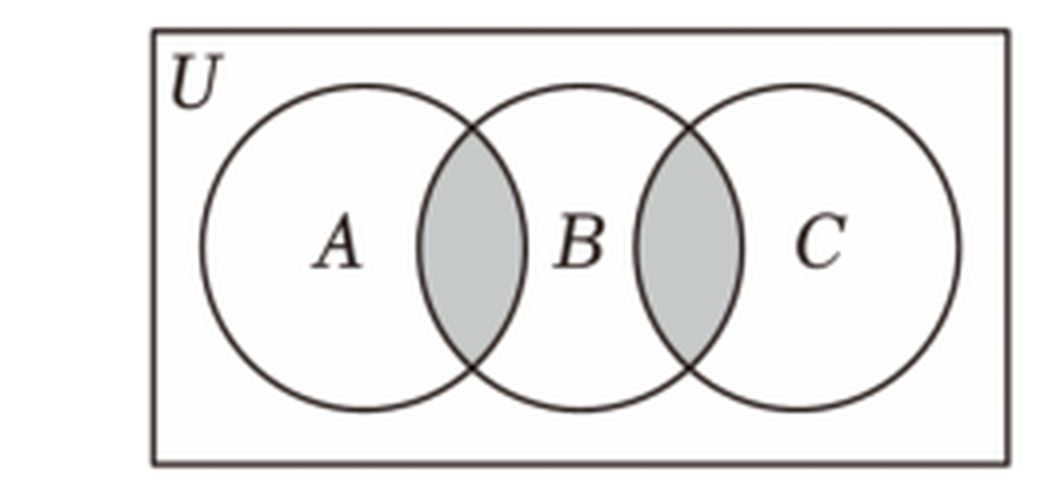
\includegraphics[width=0.30\textwidth]{figures/venn_ABC_lenses.png}
\end{center}

\keepwithprev
A. $B\cap(A\cup C)$\qquad\qquad\qquad B. $B\cap(A\cap C)$

C. $B\cap\complement_U(A\cup C)$\qquad\qquad D. $(A\cup B)\cap(B\cup C)$

\ans{$A$}

\ifanswer
\solbegin
\step{由图中阴影部分得，阴影为集合 $A$、$B$ 的交集和 $B$、$C$ 的交集的并集，}
\step{故阴影部分可表示为 $(A\cap B)\cup(B\cap C)$ 或 $B\cap(A\cup C)$，
故 $A$ 正确. 故选 $A$.}
\solend

\fi

\item 设集合 $P_1=\{x\mid x^2+ax+1>0\}$，$P_2=\{x\mid x^2+ax+2>0\}$，
$Q_1=\{x\mid x^2+x+b>0\}$，$Q_2=\{x\mid x^2+2x+b>0\}$，其中 $a$、$b\in\R$，
对于下列两个命题：①存在 $a$，$P_1$ 不是 $P_2$ 的子集；②存在 $b$ 使得 $Q_1$ 是 $Q_2$
的子集. 下列说法正确的是\mbox{（\quad）}

\keepwithprev
A. ①是真命题，②是假命题\qquad B. ①是假命题，②是真命题

C. ①②都是真命题\qquad\qquad\quad D. ①②都是假命题

\ans{$B$}

\ifanswer
\solbegin
\step{对于集合 $P_1=\{x\mid x^2+ax+1>0\}$，$P_2=\{x\mid x^2+ax+2>0\}$，}
\step{得当 $m\in P_1$ 时，即 $m^2+am+1>0$，得 $m^2+am+2>0$，}
\step{即有 $m\in P_2$，得对任意 $a$，$P_1$ 是 $P_2$ 的子集，故①错误；}
\step{对于集合 $Q_1=\{x\mid x^2+x+b>0\}$，$Q_2=\{x\mid x^2+2x+b>0\}$，}
\step{当 $b=6$ 时，$Q_1=\{x\mid x^2+x+6>0\}=\R$，$Q_2=\{x\mid x^2+2x+6>0\}=\R$，}
\step{得 $Q_1$ 是 $Q_2$ 的子集，所以存在 $b$，使得 $Q_1$ 是 $Q_2$ 的子集，故②正确；}
\step{故选 $B$.}
\solend

\fi

\item 设 $a$、$b\in\R$，则“$a+b>2$ 且 $ab>1$”是“$a>1$ 且 $b>1$”的\mbox{（\quad）}

\keepwithprev
A. 充要条件\qquad\qquad\qquad B. 充分不必要条件

C. 必要不充分条件\qquad\quad D. 既不充分又不必要条件

\ans{$C$}

\ifanswer
\solbegin
\step{因为 $a>1$ 且 $b>1$，所以 $a+b>2$ 且 $ab>1$，}
\step{若已知 $a+b>2$ 且 $ab>1$，可取 $a=\dfrac12$，$b=8$，也满足已知，}
\step{所以“$a+b>2$ 且 $ab>1$”是“$a>1$ 且 $b>1$”的必要不充分条件，故选 $C$.}
\solend

\fi

\item 十七世纪，数学家费马提出猜想：“对任意正整数 $n>2$，关于 $x$、$y$、$z$ 的方程
$x^n+y^n=z^n$ 没有正整数解”. 1995 年数学家安德鲁·怀尔斯发表了完成的证明过程，使它
终成费马大定理. 对费马大定理，若用反证法证明，第一步是假设猜想不成立，即\mbox{（\quad）}

\keepwithprev
A. 对任意正整数 $n>2$，关于 $x$、$y$、$z$ 的方程 $x^n+y^n=z^n$ 都有正整数解

B. 对任意正整数 $n>2$，关于 $x$、$y$、$z$ 的方程 $x^n+y^n=z^n$ 至少存在一组正整数解

C. 存在正整数 $n\leqslant2$，关于 $x$、$y$、$z$ 的方程 $x^n+y^n=z^n$ 至少存在一组正整数解

D. 存在正整数 $n>2$，关于 $x$、$y$、$z$ 的方程 $x^n+y^n=z^n$ 至少存在一组正整数解

\ans{$D$}

\end{enumerate}

\bigsec{三、解答题}

\begin{enumerate}
\setcounter{enumi}{16}

\item 已知 $a$、$b$、$c$ 都是实数，且 $a+b+c=0$，$abc=1$，求证：$a$、$b$、$c$ 中必有一个
大于 $\dfrac32$.

\ifanswer
\solbegin
\step{由 $a+b+c=0$，$abc=1$，得 $a$、$b$、$c$ 中一个正数，两个负数，}
\step{不妨设 $c>0$，由题意得 $a+b=-c,ab=\dfrac1c$，}
\step{由根与系数的关系得 $a$、$b$ 是关于 $x$ 的方程 $x^2+cx+\dfrac1c=0$ 的两个根，}
\step{则 $\Delta=c^2-\dfrac4c=\dfrac{c^3-4}{c}\geqslant0$，}
\step{因为 $c>0$，所以 $c^3\geqslant4$，得 $c\geqslant\sqrt[3]{4}$，}
\step{又 $\dfrac32=\sqrt[3]{\left(\dfrac32\right)^3}=\sqrt[3]{\dfrac{27}{8}}<\sqrt[3]{4}$，}
\step{所以 $c>\dfrac32$，即 $a$、$b$、$c$ 中必有一个大于 $\dfrac32$.}
\solend

\fi

\ansspace[6]

\item 已知关于 $x$ 的一元二次方程 $x^2-mx+4m^2-3=0$ 的两个实根分别为 $x_1,x_2$.

\begin{enumerate}[label=(\arabic*)]
\item $x_1,x_2$ 均为正根，求实数 $m$ 的取值范围；
\item 若 $x_1,x_2$ 满足：$x_1+x_2=x_1x_2$，求实数 $m$ 的值.
\end{enumerate}

\ifanswer
\solbegin
\stepm{(1)}{由 $x_1,x_2$ 均为正根，得}
\step{$\begin{cases}\Delta=(-m)^2-4(4m^2-3)\geqslant0\\ x_1+x_2=m>0\\ x_1\cdot x_2=4m^2-3>0\end{cases}$，}
\step{解得 $\begin{cases}-\dfrac{2\sqrt5}{5}\leqslant m\leqslant\dfrac{2\sqrt5}{5}\\[4pt]
m>0\\[4pt] m\leqslant-\dfrac{\sqrt3}{2}$ 或 $m\geqslant\dfrac{\sqrt3}{2}\end{cases}$，}
\step{即 $\dfrac{\sqrt3}{2}\leqslant m\leqslant\dfrac{2\sqrt5}{5}$；}
\stepm{(2)}{由 (1) 得
$\begin{cases}-\dfrac{2\sqrt5}{5}\leqslant m\leqslant\dfrac{2\sqrt5}{5}\\[4pt]
m=4m^2-3\end{cases}$，解得 $m=1$（舍去）或 $m=-\dfrac34$，}
\step{则 $m=-\dfrac34$.}
\solend

\fi

\ansspace[6]

\item 已知集合 $A=\{x\mid m-1<x<m^2+1\}$，$B=\{x\mid-2<x<2\}$.

\begin{enumerate}[label=(\arabic*)]
\item 当 $m=2$ 时，求 $A\cup B$、$A\cap B$、$\complement_R B$、$A\cap(\complement_R B)$；
\item 若“$x\in A$”是“$x\in B$”成立的必要不充分条件，求实数 $m$ 的取值范围.
\end{enumerate}

\ifanswer
\solbegin
\stepm{(1)}{$m=2$ 时，$A=\{x\mid1<x<5\}$，且 $B=\{x\mid-2<x<2\}$，}
\step{所以 $A\cup B=\{x\mid-2<x<5\}$，$A\cap B=\{x\mid1<x<2\}$，}
\step{$\complement_R B=\{x\mid x\leqslant-2$ 或 $x\geqslant2\}$，
$A\cap(\complement_R B)=\{x\mid2\leqslant x<5\}$；}
\stepm{(2)}{若“$x\in A$”是“$x\in B$”成立的必要不充分条件，则 $B\subset A$，}
\step{所以 $\begin{cases}m-1<-2\\ m^2+1\geqslant2\end{cases}$
或 $\begin{cases}m-1\leqslant-2\\ m^2+1>2\end{cases}$，解得 $m<-1$，}
\step{故 $m$ 的取值范围为 $(-\infty,-1)$.}
\solend

\fi

\ansspace[6]

\item 已知 $m\in\R$，集合 $A=\{x\mid|x-1|\leqslant2\}$，集合
$B=\{x\mid m-3<x\leqslant m+2\}$.

\begin{enumerate}[label=(\arabic*)]
\item 若“$x\in A$”是“$x\in B$”的充分不必要条件，求 $m$ 的取值范围；
\item 若命题“$\forall x\in B$，$x\in\complement_R A$”是真命题，求 $m$ 的取值范围；
\item 若命题“$\exists x\in A$，$x\in B$”是真命题，求 $m$ 的取值范围.
\end{enumerate}

\ifanswer
\solbegin
\stepm{(1)}{集合 $A=\{x\mid|x-1|\leqslant2\}=\{x\mid-1\leqslant x\leqslant3\}$，}
\step{若“$x\in A$”是“$x\in B$”的充分不必要条件，则 $A\subset B$，}
\step{所以 $\begin{cases}m-3<-1\\ 3\leqslant m+2\end{cases}$，解得 $1\leqslant m<2$，}
\step{当 $m=1$ 时，$B=\{x\mid-2<x\leqslant3\}$，符合题意，}
\step{所以 $m$ 的取值范围是 $\{m\mid1\leqslant m<2\}$.}
\stepm{(2)}{若命题“$\forall x\in B$，$x\in\complement_R A$”是真命题，则 $B\subset\complement_R A$，}
\step{又 $\complement_R A=\{x\mid x<-1$ 或 $x>3\}$，$B\neq\varnothing$，
所以 $m+2<-1$ 或 $m-3\geqslant3$，}
\step{解得 $m<-3$ 或 $m\geqslant6$，所以 $\{m\mid m<-3$ 或 $m\geqslant6\}$；}
\stepm{(3)}{因为 $\exists x\in A$，$x\in B$ 是真命题，所以 $A\cap B\neq\varnothing$，}
\step{当 $A\cap B=\varnothing$ 时，所以 $m+2<-1$ 或 $m-3\geqslant3$，
即 $m<-3$ 或 $m\geqslant6$，}
\step{所以当 $A\cap B\neq\varnothing$ 时，$m$ 的取值范围是 $\{m\mid-3\leqslant m<6\}$，}
\step{则 $m$ 的取值范围是 $\{m\mid-3\leqslant m<6\}$.}
\solend

\fi

\ansspace[6]

\item 对于函数 $f(x)$，若 $f(x_0)=x_0$，则称 $x_0$ 为 $f(x)$ 的“不动点”；若
$f[f(x_0)]=x_0$，则称 $x_0$ 为 $f(x)$ 的“稳定点”. 函数 $f(x)$ 的“不动点”和“稳定点”
的集合分别记为 $A$ 和 $B$，即 $A=\{x\mid f(x)=x\}$，$B=\{x\mid f[f(x)]=x\}$.

\begin{enumerate}[label=(\arabic*)]
\item 设函数 $f(x)=3x+4$，求集合 $A$ 和 $B$；
\item 求证：$A\sub B$；
\item 设函数 $f(x)=ax^2+bx+c(a\neq0)$，且 $A=\varnothing$，求证：$B=\varnothing$.
\end{enumerate}

\ifanswer
\solbegin
\stepm{(1)}{令 $f(x)=3x+4=x$，解得 $x=-2$，故有 $A=\{-2\}$，}
\step{由于 $f[f(x)]=3(3x+4)+4=9x+16$，}
\step{令 $9x+16=x$，得 $x=-2$，故有 $B=\{-2\}$；}
\stepm{(2)}{若 $A=\varnothing$，则 $A\sub B$ 显然成立；}
\step{若 $A\neq\varnothing$，设 $t\in A$，则 $f(t)=t$，$f(f(t))=f(t)=t$，}
\step{所以 $t\in B$，故 $A\sub B$.}
\stepm{(3)}{因为 $A=\{x\mid f(x)=x\}=\varnothing$，所以 $ax^2+bx+c=x$ 无解，}
\step{即 $\Delta=(b-1)^2-4a<0$，}
\step{①当 $a>0$ 时，二次函数 $y=f(x)-x$，}
\step{即 $y=ax^2+(b-1)x+c$ 的图象在 $x$ 轴的上方，}
\step{所以 $\forall x\in\R$，$f(x)-x>0$ 恒成立，所以 $\forall x\in\R$，
$f(x)>x$ 恒成立，}
\step{所以 $\forall x\in\R$，$f[f(x)]>f(x)>x$ 恒成立，即 $B=\varnothing$；}
\step{②当 $a<0$ 时，同理可证 $B=\varnothing$；}
\step{综上，对于函数 $f(x)=ax^2+bx+c(a\neq0)$，当 $A=\varnothing$ 时，$B=\varnothing$.}
\solend

\fi

\ansspace*[10]

\end{enumerate}

\end{document}
"
% 紧凑版：xelatex "\def\iscompact{1}% 高一26_交附闵行_周练2.tex
%   —— 高一上数学「2026-2027 年交附闵行高一上周练 2」（试卷版/答案版）
% 试卷版：xelatex 高一26_交附闵行_周练2.tex
% 答案版：xelatex "\def\isanswer{1}% 高一26_交附闵行_周练2.tex
%   —— 高一上数学「2026-2027 年交附闵行高一上周练 2」（试卷版/答案版）
% 试卷版：xelatex 高一26_交附闵行_周练2.tex
% 答案版：xelatex "\def\isanswer{1}\input{高一26_交附闵行_周练2.tex}"
% 紧凑版：xelatex "\def\iscompact{1}\input{高一26_交附闵行_周练2.tex}"
%
% 原始材料是微信公众号图文（公众号「魔都数学加油站」连载「27学年高一 26」，2026-09-21 发布，
% 原文标题「27学年高一26——2026-2027年上海市交附闵行高一上周练2」），
% 正文为 10 张 PNG 页（1080×1527，各页同尺寸）。原文本身就是一份**讲评版**——
% 题目下方直接印出【解析】（本卷无单独的【答案】行，填空题答案都写在解析里）。
% 试题文字与解析均照原卷录入，未改内容。卷面的粉色斜水印「魔都数学加油站」属水印，未录入。
%
% 卷首标题：原卷印作「2026-2027 年交附闵行高一上周练 2」（公众号标题里的「上海市」
% 三字卷面标题行没有，本稿照卷面），年份区间按全稿惯例排 en dash，前缀照原卷保留「年」。
%
% 与原卷的排版差异（均已在 README「说明」中交代）：
%   ① 原文自**第 3 题**起（第 1、2 题未在该文中发布），故本稿题号亦自 3 起；
%   ② 原卷本就印有「一、填空题」「二、选择题」「三、解答题」三节标题，本稿照原卷分节，
%      只把标题改排成全稿统一的「大节标题」样式；
%   ③ 原卷第 16 题的答案「D」直接印在题干末尾的括号内（原卷把括号连同 D 单独占一行），
%      第 13—15 题的括号空着、答案写在解析末句「故选 A／B／C」里；填空题的答案也都嵌在
%      解析里，本稿统一改为试卷版隐去、答案版以 \ans{} 给出（选择题另附【解析】）；
%   ④ 子集符号原卷两种并用：第 4 题题干与第 8 题、第 21(2) 题等作带下划线的 $\subseteq$，
%      第 19(2)、20(1)(2) 题作真包含的 $\subset$，本稿分别照录为 $\sub$ 与 $\subset$；
%   ⑤ 补集符号原卷作 $\complement_R$、$\complement_U$（第 4 题命题④、第 13 题选项 C、
%      第 19—20 题），本稿照录；
%   ⑥ 原卷的实数集 R 一律作斜体（第 11 题「$a\in R$」、第 14 题「$a$、$b\in R$」与解析的
%      $\{x\mid x^2+x+6>0\}=R$ 等），本稿按全稿惯例统一写作 $\R$；
%   ⑦ 原卷填空的横线约两个字宽，本稿按全稿惯例统一排 \blankline[4.4em]；
%   ⑧ 原卷未印副标题，本稿按全稿惯例补出副标题「集合与常用逻辑用语」；
%   ⑨ 第 13 题的 Venn 图原卷印在题干右侧（第 5 页），本稿移至题干之后；
%      图取原卷截图、4× LANCZOS 放大（figures/venn_ABC_lenses.png，
%      阴影为 $A\cap B$ 与 $B\cap C$ 两个交带，即 $(A\cap B)\cup(B\cap C)$）。
%
% 原卷存疑一处（照抄原卷、未改，见源码中该处上方注释）：
%   ① 第 12 题【解析】首步的方程组里印 $t<2$，而其后三处与末行答案都作 $t\leqslant2$
%      （$\left[\dfrac85,\dfrac{17}{10}\right)\cup\left(\dfrac95,2\right]$ 含 $2$）——
%      按题意 $N=\left\{x\mid t-\dfrac35\leqslant x\leqslant t\right\}\sub\{x\mid1\leqslant x\leqslant2\}$
%      只要求 $t\leqslant2$（$t=2$ 时 $N=\left[\dfrac75,2\right]$ 确实含于其中），
%      故方程组里的 $t<2$ 应是原卷笔误；本稿两处都照原卷录入、未互相迁就。
% 另：第 20(3) 题解析末两行原卷即作同话重复，照原卷录入。

\documentclass[a4paper,11pt]{article}
\usepackage{common}

\begin{document}

\examtitlest[3]{2026--2027 年交附闵行高一上周练 2}{集合与常用逻辑用语}

\bigsec{一、填空题}

\begin{enumerate}
\setcounter{enumi}{2}

\item 命题甲：集合 $M=\{x\mid kx^2-2kx+1=0\}$ 为空集；命题乙：关于 $x$ 的不等式
$x^2+(k-1)x+4>0$ 的解集为 $\R$. 若命题甲、乙中有且只有一个是真命题，则实数 $k$ 的取
值范围是 \blankline[4.4em].

\ifanswer
\solbegin
\step{因为集合 $M=\{x\mid kx^2-2kx+1=0\}$ 为空集，}
\step{当 $k\neq0$ 时，$\Delta=(-2k)^2-4k<0$，解得 $0<k<1$，}
\step{当 $k=0$ 时，方程变为 $1=0$，无解，满足题意，故 $0\leqslant k<1$；}
\step{又关于 $x$ 的不等式 $x^2+(k-1)x+4>0$ 的解集为 $\R$，}
\step{所以 $\Delta'=(k-1)^2-4\times4<0$，解得 $-3<k<5$，}
\step{当甲命题为真，乙命题为假时，无解，}
\step{当甲命题为假，乙命题为真时，$k\in(-3,0)\cup[1,5)$.}
\solend

\fi

\item 对任意 $A$、$B\sub\R$，记 $A\oplus B=\{x\mid x\in A\cup B,x\notin A\cap B\}$，
并称 $A\oplus B$ 为集合 $A$、$B$ 的对称差. 例如：若 $A=\{1,2,3\},B=\{2,3,4\}$，
则 $A\oplus B=\{1,4\}$. 下列命题中，为真命题的是 \blankline[4.4em].

\keepwithprev
①若 $A$、$B\sub\R$ 且 $A\oplus B\sub A$，则 $A\sub B$

②若 $A$、$B\sub\R$ 且 $A\oplus B=\varnothing$，则 $A=B$

③若 $A$、$B\sub\R$ 且 $A\oplus B=B$，则 $A=\varnothing$

④对任意 $A$、$B\sub\R$，都有 $A\oplus B=\complement_R A\oplus\complement_R B$

\ans{②③④}

\ifanswer
\solbegin
\step{对于①，因为 $A\oplus B\sub A$，
所以 $\{x\mid x\in A\cup B,x\notin A\cap B\}\sub A$，}
\step{故 $B\sub A$，①错误；}
\step{对于②，$A$、$B\sub\R$ 且 $A\oplus B=\varnothing$，
则 $\varnothing=\{x\mid x\in A\cup B,x\notin A\cap B\}$，}
\step{即 $A\cup B=A\cap B$，所以 $A=B$，②正确；}
\step{对于③，$A$、$B\sub\R$ 且 $A\oplus B=B$，
则 $B=\{x\mid x\in A\cup B,x\notin A\cap B\}$，}
\step{故 $A\sub B$，且 $B$ 中元素不在 $A\cap B$ 中，故 $A=\varnothing$，③正确；}
\step{对于④，$\complement_R A\oplus\complement_R B
=\{x\mid x\in\complement_R A\cup\complement_R B,x\notin\complement_R A\cap\complement_R B\}$，}
\step{其中 $\complement_R A\cup\complement_R B=\complement_R(A\cap B)$，
$\complement_R A\cap\complement_R B=\complement_R(A\cup B)$，}
\step{故 $\complement_R A\oplus\complement_R B
=\{x\mid x\in\complement_R(A\cap B),x\notin\complement_R(A\cup B)\}
=\{x\mid x\in A\cup B,x\notin A\cap B\}$，}
\step{而 $A\oplus B=\{x\mid x\in A\cup B,x\notin A\cap B\}$，
故 $A\oplus B=\complement_R A\oplus\complement_R B$，④正确.}
\step{故正确的是②③④.}
\solend

\fi

\item 已知 $A=\{a_1,a_2,a_3,a_4\},B=\{a^2\mid a\in A\}$，其中 $a_1<a_2<a_3<a_4$，
且 $a_1$、$a_2$、$a_3$、$a_4$ 均为整数，若 $A\cap B=\{a_3,a_4\},a_1+a_3=0$，
且 $A\cup B$ 中的所有元素之和为 $270$，则集合 $A$ 中所有元素之和为 \blankline[4.4em].

\ifanswer
\solbegin
\step{$A=\{a_1,a_2,a_3,a_4\},B=\{a^2\mid a\in A\}$，
因为 $A\cap B=\{a_3,a_4\},a_1+a_3=0$，}
\step{所以 $A=\{a_1,a_2,a_3,a_4\},B=\left\{a_1^2,a_2^2,a_4^2\right\}$，}
\step{若 $a_1^2=a_3$，则 $a_1=-1,a_3=1$，则 $a_2=0$，
此时 $A=\{-1,0,1,a_4\},B=\{0,1,a_4^2\}$，}
\step{因为 $A\cup B$ 中的所有元素之和为 $270$，
所以 $-1+0+1+a_4+1+a_4^2=270$，}
\step{无正整数解，舍去；}
\step{若 $a_2^2=a_3$，① $a_4^2=a_4$，所以 $a_4=1$，矛盾；}
\step{② $a_1^2=a_4$，此时 $A\cup B=\left\{-a_2^2,a_2,a_2^2,a_1^2,a_4^2\right\}$，
所以 $a_2^8+a_2^4+a_2=270$，}
\step{所以 $a_2=-2$，此时 $a_1=-4,a_2=-2,a_3=4,a_4=16$；}
\step{若 $a_4^2=a_3$，显然不成立；}
\step{综上，集合 $A$ 中所有元素之和为 $-4-2+4+16=14$.}
\solend

\fi

\item 将集合 $M=\{a_1,a_2,a_3,\cdots,a_n\}$ 分拆成两个集合 $A_i$ 和 $B_j$，且
$M\supseteq A_i\cup B_j$，$A_i\cap B_j=\varnothing$，这样的分拆方法共有 \blankline[4.4em] 种.

\ifanswer
\solbegin
\step{按集合 $A_i$ 中的元素个数进行分类：}
\step{若 $A_i$ 中有 $0$ 个元素（即 $C_n^0$ 种）时，则 $B_j$ 有 $2^n$ 种，
共有 $2^nC_n^0$ 种；}
\step{若 $A_i$ 中有 $1$ 个元素（即 $C_n^1$ 种）时，则 $B_j$ 有 $2^{n-1}$ 种，
共有 $2^{n-1}C_n^1$ 种；}
\step{若 $A_i$ 中有 $2$ 个元素（即 $C_n^2$ 种）时，则 $B_j$ 有 $2^{n-2}$ 种，
共有 $2^{n-2}C_n^2$ 种；}
\step{若 $A_i$ 中有 $3$ 个元素（即 $C_n^3$ 种）时，则 $B_j$ 有 $2^{n-3}$ 种，
共有 $2^{n-3}C_n^3$ 种；}
\step{若 $A_i$ 中有 $n$ 个元素（即 $C_n^n$ 种）时，则 $B_j$ 有 $2^0$ 种，
共有 $2^0C_n^n$ 种；}
\step{得 $2^nC_n^0+2^{n-1}C_n^1+2^{n-2}C_n^2+\cdots+2^0C_n^n=(1+2)^n$，
故这样的分拆方法有 $3^n$ 种.}
\solend

\fi

\item 已知集合 $A=\{x\mid x<2,x\in\Z\}$，$B=\{x\mid x>0,x\in\Z\}$，则
$A\cap B=$ \blankline[4.4em].

\ifanswer
\solbegin
\step{因为 $A=\{x\mid x<2,x\in\Z\}$，$B=\{x\mid x>0,x\in\Z\}$，}
\step{所以 $A\cap B=\{x\mid0<x<2,x\in\Z\}=\{1\}$.}
\solend

\fi

\item 已知集合 $A=\{x\mid(a-1)x^2+3x-2=0\}$，$B=\{x\mid x^2-3x+2=0\}$，若
$A\sub B$，求实数 $a$ 的取值范围是 \blankline[4.4em].

\ifanswer
\solbegin
\step{由方程 $x^2-3x+2=0$，解得 $x=1$ 或 $x=2$，即 $B=\{1,2\}$，}
\step{因为 $A\sub B$，所以 $A=\varnothing$ 或 $A=\{1\}$ 或 $A=\{2\}$ 或 $A=\{1,2\}$，}
\step{当 $A=\varnothing$ 时，
则 $\begin{cases}a\neq1\\ \Delta=3^2-4(a-1)\times(-2)<0\end{cases}$，
解得 $a<-\dfrac18$；}
\step{将 $x=1$ 代入方程 $(a-1)x^2+3x-2=0$，得 $a=0$，}
\step{此时 $A=\{x\mid-x^2+3x-2=0\}=\{1,2\}$，满足条件；}
\step{将 $x=2$ 代入方程 $(a-1)x^2+3x-2=0$，得到 $a=0$，上面已经验证满足条件；}
\step{综上所述，$a$ 的取值范围是 $\left(-\infty,-\dfrac18\right)\cup\{0\}$.}
\solend

\fi

\item 已知方程 $x^2-3x+a=0$ 的两根都大于 $1$，则 $a$ 的取值范围为 \blankline[4.4em].

\ifanswer
\solbegin
\step{由题意得 $\Delta=9-4a\geqslant0$，$x_1+x_2=3$，$x_1x_2=a$，
所以 $a\leqslant\dfrac94$，}
\step{则 $(x_1-1)(x_2-1)=x_1x_2-(x_1+x_2)+1=a-3+1>0$，所以 $a>2$，}
\step{故 $a$ 的范围为 $\left(2,\dfrac94\right]$.}
\solend

\fi

\item 设 $x_1$、$x_2$ 是方程 $x^2+x-3=0$ 的两个实数根，则 $x_1^2-x_2+2024=$
\blankline[4.4em].

\ifanswer
\solbegin
\step{由题意得 $x_1^2=3-x_1$，$x_1+x_2=-1$，}
\step{则 $x_1^2-x_2+2024=3-x_1-x_2+2024=2027-(-1)=2028$.}
\solend

\fi

\item 已知 $a\in\R$，若关于 $x$ 的方程 $x^2+ax+a^2-8=0$ 有两个实根 $x_1$、$x_2$，且
$\dfrac1{x_1}+\dfrac1{x_2}=-\dfrac12$，则 $a$ 的值为 \blankline[4.4em].

\ifanswer
\solbegin
\step{由题意得 $\Delta=a^2-4(a^2-8)=32-3a^2\geqslant0$，
解得 $a^2\leqslant\dfrac{32}{3}$，}
\step{由韦达定理得 $x_1+x_2=-a$，$x_1x_2=a^2-8$，}
\step{则 $\dfrac1{x_1}+\dfrac1{x_2}=\dfrac{x_1+x_2}{x_1x_2}
=\dfrac{-a}{a^2-8}=-\dfrac12$，}
\step{即 $a^2-2a-8=(a-4)(a+2)=0$，解得 $a=4$ 或 $a=-2$.}
\step{又 $a^2\leqslant\dfrac{32}{3}$，则 $a=-2$.}
\solend

\fi

\item 定义集合 $P=\{x\mid a\leqslant x\leqslant b\}$ 的“长度”是 $b-a$，其中 $a$、
$b\in\R$. 已知集合 $M=\left\{x\mid\dfrac65\leqslant x\leqslant\dfrac{17}{10}\right\}$，
$N=\left\{x\mid t-\dfrac35\leqslant x\leqslant t\right\}$，且 $M$、$N$ 都是集合
$\{x\mid1\leqslant x\leqslant2\}$ 的子集，若集合 $M\cup N$ 的“长度”大于 $\dfrac35$，
则 $t$ 的取值范围是 \blankline[4.4em].

\ifanswer
\solbegin
\step{因为 $N=\left\{x\mid t-\dfrac35\leqslant x\leqslant t\right\}$
是集合 $\{x\mid1\leqslant x\leqslant2\}$ 的子集，}
% 注：下一行方程组里的 $t<2$ 系原卷所印（本稿照录），与其后三处及末行答案的
%     $t\leqslant2$ 自相矛盾——按题意应为 $t\leqslant2$，见文件头「原卷存疑」①。
\step{所以 $\begin{cases}t-\dfrac35\geqslant1\\[2pt] t<2\end{cases}$，
解得 $\dfrac85\leqslant t\leqslant2$，}
\step{又 $M=\left\{x\mid\dfrac65\leqslant x\leqslant\dfrac{17}{10}\right\}$，
得集合 $M$ 的“长度”为 $\dfrac{17}{10}-\dfrac65=\dfrac12$，}
\step{又 $N=\left\{x\mid t-\dfrac35\leqslant x\leqslant t\right\}$，
要使集合 $M\cup N$ 的“长度”大于 $\dfrac35$，}
\step{若 $M\cup N=\left\{x\mid t-\dfrac35\leqslant x\leqslant\dfrac{17}{10}\right\}$，
则 $\dfrac{17}{10}-t+\dfrac35>\dfrac35$，所以 $t<\dfrac{17}{10}$，}
\step{又 $\dfrac85\leqslant t\leqslant2$，所以 $\dfrac85\leqslant t<\dfrac{17}{10}$；}
\step{若 $M\cup N=\left\{x\mid\dfrac65\leqslant x\leqslant t\right\}$，
则 $t-\dfrac65>\dfrac35$，所以 $t>\dfrac95$，}
\step{又 $\dfrac85\leqslant t\leqslant2$，所以 $\dfrac95<t\leqslant2$；}
\step{则 $t$ 的取值范围是 $\left[\dfrac85,\dfrac{17}{10}\right)\cup\left(\dfrac95,2\right]$.}
\solend

\fi

\end{enumerate}

% 第 13 题是「题干 + 图 + 选项」约 5.7cm 的一整块（图 0.30\textwidth、宽高比 0.477 → 高 2.29cm，
% 加题干 1 行、选项 2 行与段间距）。`\keepwithprev` 只挡得住「题干—选项」之间，挡不住
% 夹在中间的图——实测断点落在题干之后，题干孤零零留在 p1、图与四个选项整页翻到 p2
% （切页审计的 A 类）。故照 高一30 第 4 题的成例先量一次页高；**守卫要放在 `\bigsec` 之前**
% 连节标题一起量（放标题之后会把「二、选择题」孤立在页末，正是 高一40 修过的那类 B 类）。
% 7cm ＝ 节标题约 1.1cm ＋ 第 13 题那块约 5.7cm（留少量余量）。
\needvspace{7cm}
\bigsec{二、选择题}

\begin{enumerate}
\setcounter{enumi}{12}

\item 图中阴影部分用集合符号可以表示为\mbox{（\quad）}

\begin{center}
% 图取原卷截图、4× LANCZOS 放大（原卷把图印在题干右侧，本稿移至此处，见文件头⑨）。
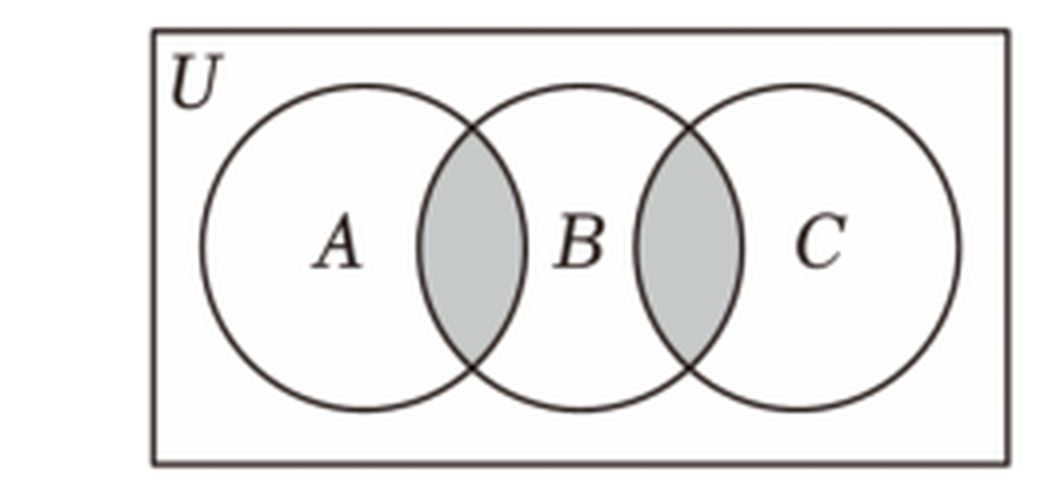
\includegraphics[width=0.30\textwidth]{figures/venn_ABC_lenses.png}
\end{center}

\keepwithprev
A. $B\cap(A\cup C)$\qquad\qquad\qquad B. $B\cap(A\cap C)$

C. $B\cap\complement_U(A\cup C)$\qquad\qquad D. $(A\cup B)\cap(B\cup C)$

\ans{$A$}

\ifanswer
\solbegin
\step{由图中阴影部分得，阴影为集合 $A$、$B$ 的交集和 $B$、$C$ 的交集的并集，}
\step{故阴影部分可表示为 $(A\cap B)\cup(B\cap C)$ 或 $B\cap(A\cup C)$，
故 $A$ 正确. 故选 $A$.}
\solend

\fi

\item 设集合 $P_1=\{x\mid x^2+ax+1>0\}$，$P_2=\{x\mid x^2+ax+2>0\}$，
$Q_1=\{x\mid x^2+x+b>0\}$，$Q_2=\{x\mid x^2+2x+b>0\}$，其中 $a$、$b\in\R$，
对于下列两个命题：①存在 $a$，$P_1$ 不是 $P_2$ 的子集；②存在 $b$ 使得 $Q_1$ 是 $Q_2$
的子集. 下列说法正确的是\mbox{（\quad）}

\keepwithprev
A. ①是真命题，②是假命题\qquad B. ①是假命题，②是真命题

C. ①②都是真命题\qquad\qquad\quad D. ①②都是假命题

\ans{$B$}

\ifanswer
\solbegin
\step{对于集合 $P_1=\{x\mid x^2+ax+1>0\}$，$P_2=\{x\mid x^2+ax+2>0\}$，}
\step{得当 $m\in P_1$ 时，即 $m^2+am+1>0$，得 $m^2+am+2>0$，}
\step{即有 $m\in P_2$，得对任意 $a$，$P_1$ 是 $P_2$ 的子集，故①错误；}
\step{对于集合 $Q_1=\{x\mid x^2+x+b>0\}$，$Q_2=\{x\mid x^2+2x+b>0\}$，}
\step{当 $b=6$ 时，$Q_1=\{x\mid x^2+x+6>0\}=\R$，$Q_2=\{x\mid x^2+2x+6>0\}=\R$，}
\step{得 $Q_1$ 是 $Q_2$ 的子集，所以存在 $b$，使得 $Q_1$ 是 $Q_2$ 的子集，故②正确；}
\step{故选 $B$.}
\solend

\fi

\item 设 $a$、$b\in\R$，则“$a+b>2$ 且 $ab>1$”是“$a>1$ 且 $b>1$”的\mbox{（\quad）}

\keepwithprev
A. 充要条件\qquad\qquad\qquad B. 充分不必要条件

C. 必要不充分条件\qquad\quad D. 既不充分又不必要条件

\ans{$C$}

\ifanswer
\solbegin
\step{因为 $a>1$ 且 $b>1$，所以 $a+b>2$ 且 $ab>1$，}
\step{若已知 $a+b>2$ 且 $ab>1$，可取 $a=\dfrac12$，$b=8$，也满足已知，}
\step{所以“$a+b>2$ 且 $ab>1$”是“$a>1$ 且 $b>1$”的必要不充分条件，故选 $C$.}
\solend

\fi

\item 十七世纪，数学家费马提出猜想：“对任意正整数 $n>2$，关于 $x$、$y$、$z$ 的方程
$x^n+y^n=z^n$ 没有正整数解”. 1995 年数学家安德鲁·怀尔斯发表了完成的证明过程，使它
终成费马大定理. 对费马大定理，若用反证法证明，第一步是假设猜想不成立，即\mbox{（\quad）}

\keepwithprev
A. 对任意正整数 $n>2$，关于 $x$、$y$、$z$ 的方程 $x^n+y^n=z^n$ 都有正整数解

B. 对任意正整数 $n>2$，关于 $x$、$y$、$z$ 的方程 $x^n+y^n=z^n$ 至少存在一组正整数解

C. 存在正整数 $n\leqslant2$，关于 $x$、$y$、$z$ 的方程 $x^n+y^n=z^n$ 至少存在一组正整数解

D. 存在正整数 $n>2$，关于 $x$、$y$、$z$ 的方程 $x^n+y^n=z^n$ 至少存在一组正整数解

\ans{$D$}

\end{enumerate}

\bigsec{三、解答题}

\begin{enumerate}
\setcounter{enumi}{16}

\item 已知 $a$、$b$、$c$ 都是实数，且 $a+b+c=0$，$abc=1$，求证：$a$、$b$、$c$ 中必有一个
大于 $\dfrac32$.

\ifanswer
\solbegin
\step{由 $a+b+c=0$，$abc=1$，得 $a$、$b$、$c$ 中一个正数，两个负数，}
\step{不妨设 $c>0$，由题意得 $a+b=-c,ab=\dfrac1c$，}
\step{由根与系数的关系得 $a$、$b$ 是关于 $x$ 的方程 $x^2+cx+\dfrac1c=0$ 的两个根，}
\step{则 $\Delta=c^2-\dfrac4c=\dfrac{c^3-4}{c}\geqslant0$，}
\step{因为 $c>0$，所以 $c^3\geqslant4$，得 $c\geqslant\sqrt[3]{4}$，}
\step{又 $\dfrac32=\sqrt[3]{\left(\dfrac32\right)^3}=\sqrt[3]{\dfrac{27}{8}}<\sqrt[3]{4}$，}
\step{所以 $c>\dfrac32$，即 $a$、$b$、$c$ 中必有一个大于 $\dfrac32$.}
\solend

\fi

\ansspace[6]

\item 已知关于 $x$ 的一元二次方程 $x^2-mx+4m^2-3=0$ 的两个实根分别为 $x_1,x_2$.

\begin{enumerate}[label=(\arabic*)]
\item $x_1,x_2$ 均为正根，求实数 $m$ 的取值范围；
\item 若 $x_1,x_2$ 满足：$x_1+x_2=x_1x_2$，求实数 $m$ 的值.
\end{enumerate}

\ifanswer
\solbegin
\stepm{(1)}{由 $x_1,x_2$ 均为正根，得}
\step{$\begin{cases}\Delta=(-m)^2-4(4m^2-3)\geqslant0\\ x_1+x_2=m>0\\ x_1\cdot x_2=4m^2-3>0\end{cases}$，}
\step{解得 $\begin{cases}-\dfrac{2\sqrt5}{5}\leqslant m\leqslant\dfrac{2\sqrt5}{5}\\[4pt]
m>0\\[4pt] m\leqslant-\dfrac{\sqrt3}{2}$ 或 $m\geqslant\dfrac{\sqrt3}{2}\end{cases}$，}
\step{即 $\dfrac{\sqrt3}{2}\leqslant m\leqslant\dfrac{2\sqrt5}{5}$；}
\stepm{(2)}{由 (1) 得
$\begin{cases}-\dfrac{2\sqrt5}{5}\leqslant m\leqslant\dfrac{2\sqrt5}{5}\\[4pt]
m=4m^2-3\end{cases}$，解得 $m=1$（舍去）或 $m=-\dfrac34$，}
\step{则 $m=-\dfrac34$.}
\solend

\fi

\ansspace[6]

\item 已知集合 $A=\{x\mid m-1<x<m^2+1\}$，$B=\{x\mid-2<x<2\}$.

\begin{enumerate}[label=(\arabic*)]
\item 当 $m=2$ 时，求 $A\cup B$、$A\cap B$、$\complement_R B$、$A\cap(\complement_R B)$；
\item 若“$x\in A$”是“$x\in B$”成立的必要不充分条件，求实数 $m$ 的取值范围.
\end{enumerate}

\ifanswer
\solbegin
\stepm{(1)}{$m=2$ 时，$A=\{x\mid1<x<5\}$，且 $B=\{x\mid-2<x<2\}$，}
\step{所以 $A\cup B=\{x\mid-2<x<5\}$，$A\cap B=\{x\mid1<x<2\}$，}
\step{$\complement_R B=\{x\mid x\leqslant-2$ 或 $x\geqslant2\}$，
$A\cap(\complement_R B)=\{x\mid2\leqslant x<5\}$；}
\stepm{(2)}{若“$x\in A$”是“$x\in B$”成立的必要不充分条件，则 $B\subset A$，}
\step{所以 $\begin{cases}m-1<-2\\ m^2+1\geqslant2\end{cases}$
或 $\begin{cases}m-1\leqslant-2\\ m^2+1>2\end{cases}$，解得 $m<-1$，}
\step{故 $m$ 的取值范围为 $(-\infty,-1)$.}
\solend

\fi

\ansspace[6]

\item 已知 $m\in\R$，集合 $A=\{x\mid|x-1|\leqslant2\}$，集合
$B=\{x\mid m-3<x\leqslant m+2\}$.

\begin{enumerate}[label=(\arabic*)]
\item 若“$x\in A$”是“$x\in B$”的充分不必要条件，求 $m$ 的取值范围；
\item 若命题“$\forall x\in B$，$x\in\complement_R A$”是真命题，求 $m$ 的取值范围；
\item 若命题“$\exists x\in A$，$x\in B$”是真命题，求 $m$ 的取值范围.
\end{enumerate}

\ifanswer
\solbegin
\stepm{(1)}{集合 $A=\{x\mid|x-1|\leqslant2\}=\{x\mid-1\leqslant x\leqslant3\}$，}
\step{若“$x\in A$”是“$x\in B$”的充分不必要条件，则 $A\subset B$，}
\step{所以 $\begin{cases}m-3<-1\\ 3\leqslant m+2\end{cases}$，解得 $1\leqslant m<2$，}
\step{当 $m=1$ 时，$B=\{x\mid-2<x\leqslant3\}$，符合题意，}
\step{所以 $m$ 的取值范围是 $\{m\mid1\leqslant m<2\}$.}
\stepm{(2)}{若命题“$\forall x\in B$，$x\in\complement_R A$”是真命题，则 $B\subset\complement_R A$，}
\step{又 $\complement_R A=\{x\mid x<-1$ 或 $x>3\}$，$B\neq\varnothing$，
所以 $m+2<-1$ 或 $m-3\geqslant3$，}
\step{解得 $m<-3$ 或 $m\geqslant6$，所以 $\{m\mid m<-3$ 或 $m\geqslant6\}$；}
\stepm{(3)}{因为 $\exists x\in A$，$x\in B$ 是真命题，所以 $A\cap B\neq\varnothing$，}
\step{当 $A\cap B=\varnothing$ 时，所以 $m+2<-1$ 或 $m-3\geqslant3$，
即 $m<-3$ 或 $m\geqslant6$，}
\step{所以当 $A\cap B\neq\varnothing$ 时，$m$ 的取值范围是 $\{m\mid-3\leqslant m<6\}$，}
\step{则 $m$ 的取值范围是 $\{m\mid-3\leqslant m<6\}$.}
\solend

\fi

\ansspace[6]

\item 对于函数 $f(x)$，若 $f(x_0)=x_0$，则称 $x_0$ 为 $f(x)$ 的“不动点”；若
$f[f(x_0)]=x_0$，则称 $x_0$ 为 $f(x)$ 的“稳定点”. 函数 $f(x)$ 的“不动点”和“稳定点”
的集合分别记为 $A$ 和 $B$，即 $A=\{x\mid f(x)=x\}$，$B=\{x\mid f[f(x)]=x\}$.

\begin{enumerate}[label=(\arabic*)]
\item 设函数 $f(x)=3x+4$，求集合 $A$ 和 $B$；
\item 求证：$A\sub B$；
\item 设函数 $f(x)=ax^2+bx+c(a\neq0)$，且 $A=\varnothing$，求证：$B=\varnothing$.
\end{enumerate}

\ifanswer
\solbegin
\stepm{(1)}{令 $f(x)=3x+4=x$，解得 $x=-2$，故有 $A=\{-2\}$，}
\step{由于 $f[f(x)]=3(3x+4)+4=9x+16$，}
\step{令 $9x+16=x$，得 $x=-2$，故有 $B=\{-2\}$；}
\stepm{(2)}{若 $A=\varnothing$，则 $A\sub B$ 显然成立；}
\step{若 $A\neq\varnothing$，设 $t\in A$，则 $f(t)=t$，$f(f(t))=f(t)=t$，}
\step{所以 $t\in B$，故 $A\sub B$.}
\stepm{(3)}{因为 $A=\{x\mid f(x)=x\}=\varnothing$，所以 $ax^2+bx+c=x$ 无解，}
\step{即 $\Delta=(b-1)^2-4a<0$，}
\step{①当 $a>0$ 时，二次函数 $y=f(x)-x$，}
\step{即 $y=ax^2+(b-1)x+c$ 的图象在 $x$ 轴的上方，}
\step{所以 $\forall x\in\R$，$f(x)-x>0$ 恒成立，所以 $\forall x\in\R$，
$f(x)>x$ 恒成立，}
\step{所以 $\forall x\in\R$，$f[f(x)]>f(x)>x$ 恒成立，即 $B=\varnothing$；}
\step{②当 $a<0$ 时，同理可证 $B=\varnothing$；}
\step{综上，对于函数 $f(x)=ax^2+bx+c(a\neq0)$，当 $A=\varnothing$ 时，$B=\varnothing$.}
\solend

\fi

\ansspace*[10]

\end{enumerate}

\end{document}
"
% 紧凑版：xelatex "\def\iscompact{1}% 高一26_交附闵行_周练2.tex
%   —— 高一上数学「2026-2027 年交附闵行高一上周练 2」（试卷版/答案版）
% 试卷版：xelatex 高一26_交附闵行_周练2.tex
% 答案版：xelatex "\def\isanswer{1}\input{高一26_交附闵行_周练2.tex}"
% 紧凑版：xelatex "\def\iscompact{1}\input{高一26_交附闵行_周练2.tex}"
%
% 原始材料是微信公众号图文（公众号「魔都数学加油站」连载「27学年高一 26」，2026-09-21 发布，
% 原文标题「27学年高一26——2026-2027年上海市交附闵行高一上周练2」），
% 正文为 10 张 PNG 页（1080×1527，各页同尺寸）。原文本身就是一份**讲评版**——
% 题目下方直接印出【解析】（本卷无单独的【答案】行，填空题答案都写在解析里）。
% 试题文字与解析均照原卷录入，未改内容。卷面的粉色斜水印「魔都数学加油站」属水印，未录入。
%
% 卷首标题：原卷印作「2026-2027 年交附闵行高一上周练 2」（公众号标题里的「上海市」
% 三字卷面标题行没有，本稿照卷面），年份区间按全稿惯例排 en dash，前缀照原卷保留「年」。
%
% 与原卷的排版差异（均已在 README「说明」中交代）：
%   ① 原文自**第 3 题**起（第 1、2 题未在该文中发布），故本稿题号亦自 3 起；
%   ② 原卷本就印有「一、填空题」「二、选择题」「三、解答题」三节标题，本稿照原卷分节，
%      只把标题改排成全稿统一的「大节标题」样式；
%   ③ 原卷第 16 题的答案「D」直接印在题干末尾的括号内（原卷把括号连同 D 单独占一行），
%      第 13—15 题的括号空着、答案写在解析末句「故选 A／B／C」里；填空题的答案也都嵌在
%      解析里，本稿统一改为试卷版隐去、答案版以 \ans{} 给出（选择题另附【解析】）；
%   ④ 子集符号原卷两种并用：第 4 题题干与第 8 题、第 21(2) 题等作带下划线的 $\subseteq$，
%      第 19(2)、20(1)(2) 题作真包含的 $\subset$，本稿分别照录为 $\sub$ 与 $\subset$；
%   ⑤ 补集符号原卷作 $\complement_R$、$\complement_U$（第 4 题命题④、第 13 题选项 C、
%      第 19—20 题），本稿照录；
%   ⑥ 原卷的实数集 R 一律作斜体（第 11 题「$a\in R$」、第 14 题「$a$、$b\in R$」与解析的
%      $\{x\mid x^2+x+6>0\}=R$ 等），本稿按全稿惯例统一写作 $\R$；
%   ⑦ 原卷填空的横线约两个字宽，本稿按全稿惯例统一排 \blankline[4.4em]；
%   ⑧ 原卷未印副标题，本稿按全稿惯例补出副标题「集合与常用逻辑用语」；
%   ⑨ 第 13 题的 Venn 图原卷印在题干右侧（第 5 页），本稿移至题干之后；
%      图取原卷截图、4× LANCZOS 放大（figures/venn_ABC_lenses.png，
%      阴影为 $A\cap B$ 与 $B\cap C$ 两个交带，即 $(A\cap B)\cup(B\cap C)$）。
%
% 原卷存疑一处（照抄原卷、未改，见源码中该处上方注释）：
%   ① 第 12 题【解析】首步的方程组里印 $t<2$，而其后三处与末行答案都作 $t\leqslant2$
%      （$\left[\dfrac85,\dfrac{17}{10}\right)\cup\left(\dfrac95,2\right]$ 含 $2$）——
%      按题意 $N=\left\{x\mid t-\dfrac35\leqslant x\leqslant t\right\}\sub\{x\mid1\leqslant x\leqslant2\}$
%      只要求 $t\leqslant2$（$t=2$ 时 $N=\left[\dfrac75,2\right]$ 确实含于其中），
%      故方程组里的 $t<2$ 应是原卷笔误；本稿两处都照原卷录入、未互相迁就。
% 另：第 20(3) 题解析末两行原卷即作同话重复，照原卷录入。

\documentclass[a4paper,11pt]{article}
\usepackage{common}

\begin{document}

\examtitlest[3]{2026--2027 年交附闵行高一上周练 2}{集合与常用逻辑用语}

\bigsec{一、填空题}

\begin{enumerate}
\setcounter{enumi}{2}

\item 命题甲：集合 $M=\{x\mid kx^2-2kx+1=0\}$ 为空集；命题乙：关于 $x$ 的不等式
$x^2+(k-1)x+4>0$ 的解集为 $\R$. 若命题甲、乙中有且只有一个是真命题，则实数 $k$ 的取
值范围是 \blankline[4.4em].

\ifanswer
\solbegin
\step{因为集合 $M=\{x\mid kx^2-2kx+1=0\}$ 为空集，}
\step{当 $k\neq0$ 时，$\Delta=(-2k)^2-4k<0$，解得 $0<k<1$，}
\step{当 $k=0$ 时，方程变为 $1=0$，无解，满足题意，故 $0\leqslant k<1$；}
\step{又关于 $x$ 的不等式 $x^2+(k-1)x+4>0$ 的解集为 $\R$，}
\step{所以 $\Delta'=(k-1)^2-4\times4<0$，解得 $-3<k<5$，}
\step{当甲命题为真，乙命题为假时，无解，}
\step{当甲命题为假，乙命题为真时，$k\in(-3,0)\cup[1,5)$.}
\solend

\fi

\item 对任意 $A$、$B\sub\R$，记 $A\oplus B=\{x\mid x\in A\cup B,x\notin A\cap B\}$，
并称 $A\oplus B$ 为集合 $A$、$B$ 的对称差. 例如：若 $A=\{1,2,3\},B=\{2,3,4\}$，
则 $A\oplus B=\{1,4\}$. 下列命题中，为真命题的是 \blankline[4.4em].

\keepwithprev
①若 $A$、$B\sub\R$ 且 $A\oplus B\sub A$，则 $A\sub B$

②若 $A$、$B\sub\R$ 且 $A\oplus B=\varnothing$，则 $A=B$

③若 $A$、$B\sub\R$ 且 $A\oplus B=B$，则 $A=\varnothing$

④对任意 $A$、$B\sub\R$，都有 $A\oplus B=\complement_R A\oplus\complement_R B$

\ans{②③④}

\ifanswer
\solbegin
\step{对于①，因为 $A\oplus B\sub A$，
所以 $\{x\mid x\in A\cup B,x\notin A\cap B\}\sub A$，}
\step{故 $B\sub A$，①错误；}
\step{对于②，$A$、$B\sub\R$ 且 $A\oplus B=\varnothing$，
则 $\varnothing=\{x\mid x\in A\cup B,x\notin A\cap B\}$，}
\step{即 $A\cup B=A\cap B$，所以 $A=B$，②正确；}
\step{对于③，$A$、$B\sub\R$ 且 $A\oplus B=B$，
则 $B=\{x\mid x\in A\cup B,x\notin A\cap B\}$，}
\step{故 $A\sub B$，且 $B$ 中元素不在 $A\cap B$ 中，故 $A=\varnothing$，③正确；}
\step{对于④，$\complement_R A\oplus\complement_R B
=\{x\mid x\in\complement_R A\cup\complement_R B,x\notin\complement_R A\cap\complement_R B\}$，}
\step{其中 $\complement_R A\cup\complement_R B=\complement_R(A\cap B)$，
$\complement_R A\cap\complement_R B=\complement_R(A\cup B)$，}
\step{故 $\complement_R A\oplus\complement_R B
=\{x\mid x\in\complement_R(A\cap B),x\notin\complement_R(A\cup B)\}
=\{x\mid x\in A\cup B,x\notin A\cap B\}$，}
\step{而 $A\oplus B=\{x\mid x\in A\cup B,x\notin A\cap B\}$，
故 $A\oplus B=\complement_R A\oplus\complement_R B$，④正确.}
\step{故正确的是②③④.}
\solend

\fi

\item 已知 $A=\{a_1,a_2,a_3,a_4\},B=\{a^2\mid a\in A\}$，其中 $a_1<a_2<a_3<a_4$，
且 $a_1$、$a_2$、$a_3$、$a_4$ 均为整数，若 $A\cap B=\{a_3,a_4\},a_1+a_3=0$，
且 $A\cup B$ 中的所有元素之和为 $270$，则集合 $A$ 中所有元素之和为 \blankline[4.4em].

\ifanswer
\solbegin
\step{$A=\{a_1,a_2,a_3,a_4\},B=\{a^2\mid a\in A\}$，
因为 $A\cap B=\{a_3,a_4\},a_1+a_3=0$，}
\step{所以 $A=\{a_1,a_2,a_3,a_4\},B=\left\{a_1^2,a_2^2,a_4^2\right\}$，}
\step{若 $a_1^2=a_3$，则 $a_1=-1,a_3=1$，则 $a_2=0$，
此时 $A=\{-1,0,1,a_4\},B=\{0,1,a_4^2\}$，}
\step{因为 $A\cup B$ 中的所有元素之和为 $270$，
所以 $-1+0+1+a_4+1+a_4^2=270$，}
\step{无正整数解，舍去；}
\step{若 $a_2^2=a_3$，① $a_4^2=a_4$，所以 $a_4=1$，矛盾；}
\step{② $a_1^2=a_4$，此时 $A\cup B=\left\{-a_2^2,a_2,a_2^2,a_1^2,a_4^2\right\}$，
所以 $a_2^8+a_2^4+a_2=270$，}
\step{所以 $a_2=-2$，此时 $a_1=-4,a_2=-2,a_3=4,a_4=16$；}
\step{若 $a_4^2=a_3$，显然不成立；}
\step{综上，集合 $A$ 中所有元素之和为 $-4-2+4+16=14$.}
\solend

\fi

\item 将集合 $M=\{a_1,a_2,a_3,\cdots,a_n\}$ 分拆成两个集合 $A_i$ 和 $B_j$，且
$M\supseteq A_i\cup B_j$，$A_i\cap B_j=\varnothing$，这样的分拆方法共有 \blankline[4.4em] 种.

\ifanswer
\solbegin
\step{按集合 $A_i$ 中的元素个数进行分类：}
\step{若 $A_i$ 中有 $0$ 个元素（即 $C_n^0$ 种）时，则 $B_j$ 有 $2^n$ 种，
共有 $2^nC_n^0$ 种；}
\step{若 $A_i$ 中有 $1$ 个元素（即 $C_n^1$ 种）时，则 $B_j$ 有 $2^{n-1}$ 种，
共有 $2^{n-1}C_n^1$ 种；}
\step{若 $A_i$ 中有 $2$ 个元素（即 $C_n^2$ 种）时，则 $B_j$ 有 $2^{n-2}$ 种，
共有 $2^{n-2}C_n^2$ 种；}
\step{若 $A_i$ 中有 $3$ 个元素（即 $C_n^3$ 种）时，则 $B_j$ 有 $2^{n-3}$ 种，
共有 $2^{n-3}C_n^3$ 种；}
\step{若 $A_i$ 中有 $n$ 个元素（即 $C_n^n$ 种）时，则 $B_j$ 有 $2^0$ 种，
共有 $2^0C_n^n$ 种；}
\step{得 $2^nC_n^0+2^{n-1}C_n^1+2^{n-2}C_n^2+\cdots+2^0C_n^n=(1+2)^n$，
故这样的分拆方法有 $3^n$ 种.}
\solend

\fi

\item 已知集合 $A=\{x\mid x<2,x\in\Z\}$，$B=\{x\mid x>0,x\in\Z\}$，则
$A\cap B=$ \blankline[4.4em].

\ifanswer
\solbegin
\step{因为 $A=\{x\mid x<2,x\in\Z\}$，$B=\{x\mid x>0,x\in\Z\}$，}
\step{所以 $A\cap B=\{x\mid0<x<2,x\in\Z\}=\{1\}$.}
\solend

\fi

\item 已知集合 $A=\{x\mid(a-1)x^2+3x-2=0\}$，$B=\{x\mid x^2-3x+2=0\}$，若
$A\sub B$，求实数 $a$ 的取值范围是 \blankline[4.4em].

\ifanswer
\solbegin
\step{由方程 $x^2-3x+2=0$，解得 $x=1$ 或 $x=2$，即 $B=\{1,2\}$，}
\step{因为 $A\sub B$，所以 $A=\varnothing$ 或 $A=\{1\}$ 或 $A=\{2\}$ 或 $A=\{1,2\}$，}
\step{当 $A=\varnothing$ 时，
则 $\begin{cases}a\neq1\\ \Delta=3^2-4(a-1)\times(-2)<0\end{cases}$，
解得 $a<-\dfrac18$；}
\step{将 $x=1$ 代入方程 $(a-1)x^2+3x-2=0$，得 $a=0$，}
\step{此时 $A=\{x\mid-x^2+3x-2=0\}=\{1,2\}$，满足条件；}
\step{将 $x=2$ 代入方程 $(a-1)x^2+3x-2=0$，得到 $a=0$，上面已经验证满足条件；}
\step{综上所述，$a$ 的取值范围是 $\left(-\infty,-\dfrac18\right)\cup\{0\}$.}
\solend

\fi

\item 已知方程 $x^2-3x+a=0$ 的两根都大于 $1$，则 $a$ 的取值范围为 \blankline[4.4em].

\ifanswer
\solbegin
\step{由题意得 $\Delta=9-4a\geqslant0$，$x_1+x_2=3$，$x_1x_2=a$，
所以 $a\leqslant\dfrac94$，}
\step{则 $(x_1-1)(x_2-1)=x_1x_2-(x_1+x_2)+1=a-3+1>0$，所以 $a>2$，}
\step{故 $a$ 的范围为 $\left(2,\dfrac94\right]$.}
\solend

\fi

\item 设 $x_1$、$x_2$ 是方程 $x^2+x-3=0$ 的两个实数根，则 $x_1^2-x_2+2024=$
\blankline[4.4em].

\ifanswer
\solbegin
\step{由题意得 $x_1^2=3-x_1$，$x_1+x_2=-1$，}
\step{则 $x_1^2-x_2+2024=3-x_1-x_2+2024=2027-(-1)=2028$.}
\solend

\fi

\item 已知 $a\in\R$，若关于 $x$ 的方程 $x^2+ax+a^2-8=0$ 有两个实根 $x_1$、$x_2$，且
$\dfrac1{x_1}+\dfrac1{x_2}=-\dfrac12$，则 $a$ 的值为 \blankline[4.4em].

\ifanswer
\solbegin
\step{由题意得 $\Delta=a^2-4(a^2-8)=32-3a^2\geqslant0$，
解得 $a^2\leqslant\dfrac{32}{3}$，}
\step{由韦达定理得 $x_1+x_2=-a$，$x_1x_2=a^2-8$，}
\step{则 $\dfrac1{x_1}+\dfrac1{x_2}=\dfrac{x_1+x_2}{x_1x_2}
=\dfrac{-a}{a^2-8}=-\dfrac12$，}
\step{即 $a^2-2a-8=(a-4)(a+2)=0$，解得 $a=4$ 或 $a=-2$.}
\step{又 $a^2\leqslant\dfrac{32}{3}$，则 $a=-2$.}
\solend

\fi

\item 定义集合 $P=\{x\mid a\leqslant x\leqslant b\}$ 的“长度”是 $b-a$，其中 $a$、
$b\in\R$. 已知集合 $M=\left\{x\mid\dfrac65\leqslant x\leqslant\dfrac{17}{10}\right\}$，
$N=\left\{x\mid t-\dfrac35\leqslant x\leqslant t\right\}$，且 $M$、$N$ 都是集合
$\{x\mid1\leqslant x\leqslant2\}$ 的子集，若集合 $M\cup N$ 的“长度”大于 $\dfrac35$，
则 $t$ 的取值范围是 \blankline[4.4em].

\ifanswer
\solbegin
\step{因为 $N=\left\{x\mid t-\dfrac35\leqslant x\leqslant t\right\}$
是集合 $\{x\mid1\leqslant x\leqslant2\}$ 的子集，}
% 注：下一行方程组里的 $t<2$ 系原卷所印（本稿照录），与其后三处及末行答案的
%     $t\leqslant2$ 自相矛盾——按题意应为 $t\leqslant2$，见文件头「原卷存疑」①。
\step{所以 $\begin{cases}t-\dfrac35\geqslant1\\[2pt] t<2\end{cases}$，
解得 $\dfrac85\leqslant t\leqslant2$，}
\step{又 $M=\left\{x\mid\dfrac65\leqslant x\leqslant\dfrac{17}{10}\right\}$，
得集合 $M$ 的“长度”为 $\dfrac{17}{10}-\dfrac65=\dfrac12$，}
\step{又 $N=\left\{x\mid t-\dfrac35\leqslant x\leqslant t\right\}$，
要使集合 $M\cup N$ 的“长度”大于 $\dfrac35$，}
\step{若 $M\cup N=\left\{x\mid t-\dfrac35\leqslant x\leqslant\dfrac{17}{10}\right\}$，
则 $\dfrac{17}{10}-t+\dfrac35>\dfrac35$，所以 $t<\dfrac{17}{10}$，}
\step{又 $\dfrac85\leqslant t\leqslant2$，所以 $\dfrac85\leqslant t<\dfrac{17}{10}$；}
\step{若 $M\cup N=\left\{x\mid\dfrac65\leqslant x\leqslant t\right\}$，
则 $t-\dfrac65>\dfrac35$，所以 $t>\dfrac95$，}
\step{又 $\dfrac85\leqslant t\leqslant2$，所以 $\dfrac95<t\leqslant2$；}
\step{则 $t$ 的取值范围是 $\left[\dfrac85,\dfrac{17}{10}\right)\cup\left(\dfrac95,2\right]$.}
\solend

\fi

\end{enumerate}

% 第 13 题是「题干 + 图 + 选项」约 5.7cm 的一整块（图 0.30\textwidth、宽高比 0.477 → 高 2.29cm，
% 加题干 1 行、选项 2 行与段间距）。`\keepwithprev` 只挡得住「题干—选项」之间，挡不住
% 夹在中间的图——实测断点落在题干之后，题干孤零零留在 p1、图与四个选项整页翻到 p2
% （切页审计的 A 类）。故照 高一30 第 4 题的成例先量一次页高；**守卫要放在 `\bigsec` 之前**
% 连节标题一起量（放标题之后会把「二、选择题」孤立在页末，正是 高一40 修过的那类 B 类）。
% 7cm ＝ 节标题约 1.1cm ＋ 第 13 题那块约 5.7cm（留少量余量）。
\needvspace{7cm}
\bigsec{二、选择题}

\begin{enumerate}
\setcounter{enumi}{12}

\item 图中阴影部分用集合符号可以表示为\mbox{（\quad）}

\begin{center}
% 图取原卷截图、4× LANCZOS 放大（原卷把图印在题干右侧，本稿移至此处，见文件头⑨）。
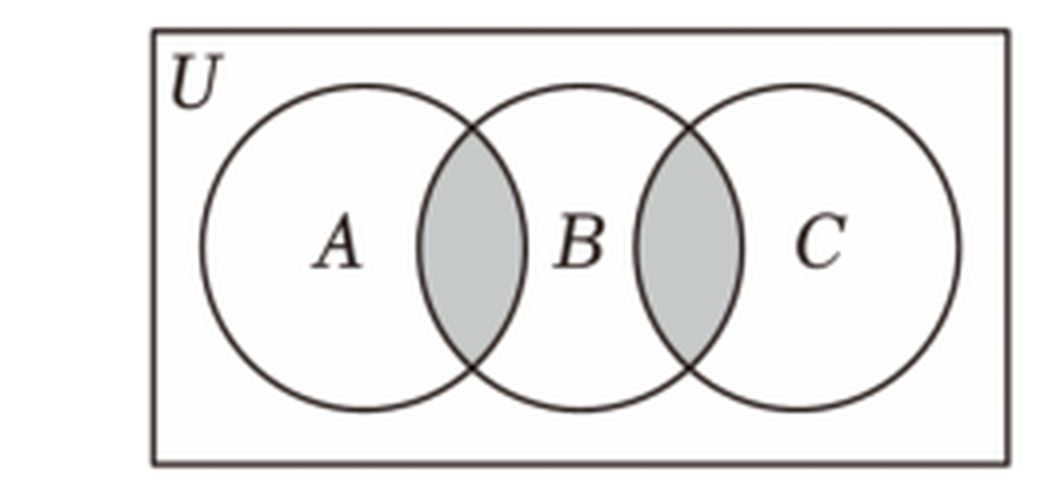
\includegraphics[width=0.30\textwidth]{figures/venn_ABC_lenses.png}
\end{center}

\keepwithprev
A. $B\cap(A\cup C)$\qquad\qquad\qquad B. $B\cap(A\cap C)$

C. $B\cap\complement_U(A\cup C)$\qquad\qquad D. $(A\cup B)\cap(B\cup C)$

\ans{$A$}

\ifanswer
\solbegin
\step{由图中阴影部分得，阴影为集合 $A$、$B$ 的交集和 $B$、$C$ 的交集的并集，}
\step{故阴影部分可表示为 $(A\cap B)\cup(B\cap C)$ 或 $B\cap(A\cup C)$，
故 $A$ 正确. 故选 $A$.}
\solend

\fi

\item 设集合 $P_1=\{x\mid x^2+ax+1>0\}$，$P_2=\{x\mid x^2+ax+2>0\}$，
$Q_1=\{x\mid x^2+x+b>0\}$，$Q_2=\{x\mid x^2+2x+b>0\}$，其中 $a$、$b\in\R$，
对于下列两个命题：①存在 $a$，$P_1$ 不是 $P_2$ 的子集；②存在 $b$ 使得 $Q_1$ 是 $Q_2$
的子集. 下列说法正确的是\mbox{（\quad）}

\keepwithprev
A. ①是真命题，②是假命题\qquad B. ①是假命题，②是真命题

C. ①②都是真命题\qquad\qquad\quad D. ①②都是假命题

\ans{$B$}

\ifanswer
\solbegin
\step{对于集合 $P_1=\{x\mid x^2+ax+1>0\}$，$P_2=\{x\mid x^2+ax+2>0\}$，}
\step{得当 $m\in P_1$ 时，即 $m^2+am+1>0$，得 $m^2+am+2>0$，}
\step{即有 $m\in P_2$，得对任意 $a$，$P_1$ 是 $P_2$ 的子集，故①错误；}
\step{对于集合 $Q_1=\{x\mid x^2+x+b>0\}$，$Q_2=\{x\mid x^2+2x+b>0\}$，}
\step{当 $b=6$ 时，$Q_1=\{x\mid x^2+x+6>0\}=\R$，$Q_2=\{x\mid x^2+2x+6>0\}=\R$，}
\step{得 $Q_1$ 是 $Q_2$ 的子集，所以存在 $b$，使得 $Q_1$ 是 $Q_2$ 的子集，故②正确；}
\step{故选 $B$.}
\solend

\fi

\item 设 $a$、$b\in\R$，则“$a+b>2$ 且 $ab>1$”是“$a>1$ 且 $b>1$”的\mbox{（\quad）}

\keepwithprev
A. 充要条件\qquad\qquad\qquad B. 充分不必要条件

C. 必要不充分条件\qquad\quad D. 既不充分又不必要条件

\ans{$C$}

\ifanswer
\solbegin
\step{因为 $a>1$ 且 $b>1$，所以 $a+b>2$ 且 $ab>1$，}
\step{若已知 $a+b>2$ 且 $ab>1$，可取 $a=\dfrac12$，$b=8$，也满足已知，}
\step{所以“$a+b>2$ 且 $ab>1$”是“$a>1$ 且 $b>1$”的必要不充分条件，故选 $C$.}
\solend

\fi

\item 十七世纪，数学家费马提出猜想：“对任意正整数 $n>2$，关于 $x$、$y$、$z$ 的方程
$x^n+y^n=z^n$ 没有正整数解”. 1995 年数学家安德鲁·怀尔斯发表了完成的证明过程，使它
终成费马大定理. 对费马大定理，若用反证法证明，第一步是假设猜想不成立，即\mbox{（\quad）}

\keepwithprev
A. 对任意正整数 $n>2$，关于 $x$、$y$、$z$ 的方程 $x^n+y^n=z^n$ 都有正整数解

B. 对任意正整数 $n>2$，关于 $x$、$y$、$z$ 的方程 $x^n+y^n=z^n$ 至少存在一组正整数解

C. 存在正整数 $n\leqslant2$，关于 $x$、$y$、$z$ 的方程 $x^n+y^n=z^n$ 至少存在一组正整数解

D. 存在正整数 $n>2$，关于 $x$、$y$、$z$ 的方程 $x^n+y^n=z^n$ 至少存在一组正整数解

\ans{$D$}

\end{enumerate}

\bigsec{三、解答题}

\begin{enumerate}
\setcounter{enumi}{16}

\item 已知 $a$、$b$、$c$ 都是实数，且 $a+b+c=0$，$abc=1$，求证：$a$、$b$、$c$ 中必有一个
大于 $\dfrac32$.

\ifanswer
\solbegin
\step{由 $a+b+c=0$，$abc=1$，得 $a$、$b$、$c$ 中一个正数，两个负数，}
\step{不妨设 $c>0$，由题意得 $a+b=-c,ab=\dfrac1c$，}
\step{由根与系数的关系得 $a$、$b$ 是关于 $x$ 的方程 $x^2+cx+\dfrac1c=0$ 的两个根，}
\step{则 $\Delta=c^2-\dfrac4c=\dfrac{c^3-4}{c}\geqslant0$，}
\step{因为 $c>0$，所以 $c^3\geqslant4$，得 $c\geqslant\sqrt[3]{4}$，}
\step{又 $\dfrac32=\sqrt[3]{\left(\dfrac32\right)^3}=\sqrt[3]{\dfrac{27}{8}}<\sqrt[3]{4}$，}
\step{所以 $c>\dfrac32$，即 $a$、$b$、$c$ 中必有一个大于 $\dfrac32$.}
\solend

\fi

\ansspace[6]

\item 已知关于 $x$ 的一元二次方程 $x^2-mx+4m^2-3=0$ 的两个实根分别为 $x_1,x_2$.

\begin{enumerate}[label=(\arabic*)]
\item $x_1,x_2$ 均为正根，求实数 $m$ 的取值范围；
\item 若 $x_1,x_2$ 满足：$x_1+x_2=x_1x_2$，求实数 $m$ 的值.
\end{enumerate}

\ifanswer
\solbegin
\stepm{(1)}{由 $x_1,x_2$ 均为正根，得}
\step{$\begin{cases}\Delta=(-m)^2-4(4m^2-3)\geqslant0\\ x_1+x_2=m>0\\ x_1\cdot x_2=4m^2-3>0\end{cases}$，}
\step{解得 $\begin{cases}-\dfrac{2\sqrt5}{5}\leqslant m\leqslant\dfrac{2\sqrt5}{5}\\[4pt]
m>0\\[4pt] m\leqslant-\dfrac{\sqrt3}{2}$ 或 $m\geqslant\dfrac{\sqrt3}{2}\end{cases}$，}
\step{即 $\dfrac{\sqrt3}{2}\leqslant m\leqslant\dfrac{2\sqrt5}{5}$；}
\stepm{(2)}{由 (1) 得
$\begin{cases}-\dfrac{2\sqrt5}{5}\leqslant m\leqslant\dfrac{2\sqrt5}{5}\\[4pt]
m=4m^2-3\end{cases}$，解得 $m=1$（舍去）或 $m=-\dfrac34$，}
\step{则 $m=-\dfrac34$.}
\solend

\fi

\ansspace[6]

\item 已知集合 $A=\{x\mid m-1<x<m^2+1\}$，$B=\{x\mid-2<x<2\}$.

\begin{enumerate}[label=(\arabic*)]
\item 当 $m=2$ 时，求 $A\cup B$、$A\cap B$、$\complement_R B$、$A\cap(\complement_R B)$；
\item 若“$x\in A$”是“$x\in B$”成立的必要不充分条件，求实数 $m$ 的取值范围.
\end{enumerate}

\ifanswer
\solbegin
\stepm{(1)}{$m=2$ 时，$A=\{x\mid1<x<5\}$，且 $B=\{x\mid-2<x<2\}$，}
\step{所以 $A\cup B=\{x\mid-2<x<5\}$，$A\cap B=\{x\mid1<x<2\}$，}
\step{$\complement_R B=\{x\mid x\leqslant-2$ 或 $x\geqslant2\}$，
$A\cap(\complement_R B)=\{x\mid2\leqslant x<5\}$；}
\stepm{(2)}{若“$x\in A$”是“$x\in B$”成立的必要不充分条件，则 $B\subset A$，}
\step{所以 $\begin{cases}m-1<-2\\ m^2+1\geqslant2\end{cases}$
或 $\begin{cases}m-1\leqslant-2\\ m^2+1>2\end{cases}$，解得 $m<-1$，}
\step{故 $m$ 的取值范围为 $(-\infty,-1)$.}
\solend

\fi

\ansspace[6]

\item 已知 $m\in\R$，集合 $A=\{x\mid|x-1|\leqslant2\}$，集合
$B=\{x\mid m-3<x\leqslant m+2\}$.

\begin{enumerate}[label=(\arabic*)]
\item 若“$x\in A$”是“$x\in B$”的充分不必要条件，求 $m$ 的取值范围；
\item 若命题“$\forall x\in B$，$x\in\complement_R A$”是真命题，求 $m$ 的取值范围；
\item 若命题“$\exists x\in A$，$x\in B$”是真命题，求 $m$ 的取值范围.
\end{enumerate}

\ifanswer
\solbegin
\stepm{(1)}{集合 $A=\{x\mid|x-1|\leqslant2\}=\{x\mid-1\leqslant x\leqslant3\}$，}
\step{若“$x\in A$”是“$x\in B$”的充分不必要条件，则 $A\subset B$，}
\step{所以 $\begin{cases}m-3<-1\\ 3\leqslant m+2\end{cases}$，解得 $1\leqslant m<2$，}
\step{当 $m=1$ 时，$B=\{x\mid-2<x\leqslant3\}$，符合题意，}
\step{所以 $m$ 的取值范围是 $\{m\mid1\leqslant m<2\}$.}
\stepm{(2)}{若命题“$\forall x\in B$，$x\in\complement_R A$”是真命题，则 $B\subset\complement_R A$，}
\step{又 $\complement_R A=\{x\mid x<-1$ 或 $x>3\}$，$B\neq\varnothing$，
所以 $m+2<-1$ 或 $m-3\geqslant3$，}
\step{解得 $m<-3$ 或 $m\geqslant6$，所以 $\{m\mid m<-3$ 或 $m\geqslant6\}$；}
\stepm{(3)}{因为 $\exists x\in A$，$x\in B$ 是真命题，所以 $A\cap B\neq\varnothing$，}
\step{当 $A\cap B=\varnothing$ 时，所以 $m+2<-1$ 或 $m-3\geqslant3$，
即 $m<-3$ 或 $m\geqslant6$，}
\step{所以当 $A\cap B\neq\varnothing$ 时，$m$ 的取值范围是 $\{m\mid-3\leqslant m<6\}$，}
\step{则 $m$ 的取值范围是 $\{m\mid-3\leqslant m<6\}$.}
\solend

\fi

\ansspace[6]

\item 对于函数 $f(x)$，若 $f(x_0)=x_0$，则称 $x_0$ 为 $f(x)$ 的“不动点”；若
$f[f(x_0)]=x_0$，则称 $x_0$ 为 $f(x)$ 的“稳定点”. 函数 $f(x)$ 的“不动点”和“稳定点”
的集合分别记为 $A$ 和 $B$，即 $A=\{x\mid f(x)=x\}$，$B=\{x\mid f[f(x)]=x\}$.

\begin{enumerate}[label=(\arabic*)]
\item 设函数 $f(x)=3x+4$，求集合 $A$ 和 $B$；
\item 求证：$A\sub B$；
\item 设函数 $f(x)=ax^2+bx+c(a\neq0)$，且 $A=\varnothing$，求证：$B=\varnothing$.
\end{enumerate}

\ifanswer
\solbegin
\stepm{(1)}{令 $f(x)=3x+4=x$，解得 $x=-2$，故有 $A=\{-2\}$，}
\step{由于 $f[f(x)]=3(3x+4)+4=9x+16$，}
\step{令 $9x+16=x$，得 $x=-2$，故有 $B=\{-2\}$；}
\stepm{(2)}{若 $A=\varnothing$，则 $A\sub B$ 显然成立；}
\step{若 $A\neq\varnothing$，设 $t\in A$，则 $f(t)=t$，$f(f(t))=f(t)=t$，}
\step{所以 $t\in B$，故 $A\sub B$.}
\stepm{(3)}{因为 $A=\{x\mid f(x)=x\}=\varnothing$，所以 $ax^2+bx+c=x$ 无解，}
\step{即 $\Delta=(b-1)^2-4a<0$，}
\step{①当 $a>0$ 时，二次函数 $y=f(x)-x$，}
\step{即 $y=ax^2+(b-1)x+c$ 的图象在 $x$ 轴的上方，}
\step{所以 $\forall x\in\R$，$f(x)-x>0$ 恒成立，所以 $\forall x\in\R$，
$f(x)>x$ 恒成立，}
\step{所以 $\forall x\in\R$，$f[f(x)]>f(x)>x$ 恒成立，即 $B=\varnothing$；}
\step{②当 $a<0$ 时，同理可证 $B=\varnothing$；}
\step{综上，对于函数 $f(x)=ax^2+bx+c(a\neq0)$，当 $A=\varnothing$ 时，$B=\varnothing$.}
\solend

\fi

\ansspace*[10]

\end{enumerate}

\end{document}
"
%
% 原始材料是微信公众号图文（公众号「魔都数学加油站」连载「27学年高一 26」，2026-09-21 发布，
% 原文标题「27学年高一26——2026-2027年上海市交附闵行高一上周练2」），
% 正文为 10 张 PNG 页（1080×1527，各页同尺寸）。原文本身就是一份**讲评版**——
% 题目下方直接印出【解析】（本卷无单独的【答案】行，填空题答案都写在解析里）。
% 试题文字与解析均照原卷录入，未改内容。卷面的粉色斜水印「魔都数学加油站」属水印，未录入。
%
% 卷首标题：原卷印作「2026-2027 年交附闵行高一上周练 2」（公众号标题里的「上海市」
% 三字卷面标题行没有，本稿照卷面），年份区间按全稿惯例排 en dash，前缀照原卷保留「年」。
%
% 与原卷的排版差异（均已在 README「说明」中交代）：
%   ① 原文自**第 3 题**起（第 1、2 题未在该文中发布），故本稿题号亦自 3 起；
%   ② 原卷本就印有「一、填空题」「二、选择题」「三、解答题」三节标题，本稿照原卷分节，
%      只把标题改排成全稿统一的「大节标题」样式；
%   ③ 原卷第 16 题的答案「D」直接印在题干末尾的括号内（原卷把括号连同 D 单独占一行），
%      第 13—15 题的括号空着、答案写在解析末句「故选 A／B／C」里；填空题的答案也都嵌在
%      解析里，本稿统一改为试卷版隐去、答案版以 \ans{} 给出（选择题另附【解析】）；
%   ④ 子集符号原卷两种并用：第 4 题题干与第 8 题、第 21(2) 题等作带下划线的 $\subseteq$，
%      第 19(2)、20(1)(2) 题作真包含的 $\subset$，本稿分别照录为 $\sub$ 与 $\subset$；
%   ⑤ 补集符号原卷作 $\complement_R$、$\complement_U$（第 4 题命题④、第 13 题选项 C、
%      第 19—20 题），本稿照录；
%   ⑥ 原卷的实数集 R 一律作斜体（第 11 题「$a\in R$」、第 14 题「$a$、$b\in R$」与解析的
%      $\{x\mid x^2+x+6>0\}=R$ 等），本稿按全稿惯例统一写作 $\R$；
%   ⑦ 原卷填空的横线约两个字宽，本稿按全稿惯例统一排 \blankline[4.4em]；
%   ⑧ 原卷未印副标题，本稿按全稿惯例补出副标题「集合与常用逻辑用语」；
%   ⑨ 第 13 题的 Venn 图原卷印在题干右侧（第 5 页），本稿移至题干之后；
%      图取原卷截图、4× LANCZOS 放大（figures/venn_ABC_lenses.png，
%      阴影为 $A\cap B$ 与 $B\cap C$ 两个交带，即 $(A\cap B)\cup(B\cap C)$）。
%
% 原卷存疑一处（照抄原卷、未改，见源码中该处上方注释）：
%   ① 第 12 题【解析】首步的方程组里印 $t<2$，而其后三处与末行答案都作 $t\leqslant2$
%      （$\left[\dfrac85,\dfrac{17}{10}\right)\cup\left(\dfrac95,2\right]$ 含 $2$）——
%      按题意 $N=\left\{x\mid t-\dfrac35\leqslant x\leqslant t\right\}\sub\{x\mid1\leqslant x\leqslant2\}$
%      只要求 $t\leqslant2$（$t=2$ 时 $N=\left[\dfrac75,2\right]$ 确实含于其中），
%      故方程组里的 $t<2$ 应是原卷笔误；本稿两处都照原卷录入、未互相迁就。
% 另：第 20(3) 题解析末两行原卷即作同话重复，照原卷录入。

\documentclass[a4paper,11pt]{article}
\usepackage{common}

\begin{document}

\examtitlest[3]{2026--2027 年交附闵行高一上周练 2}{集合与常用逻辑用语}

\bigsec{一、填空题}

\begin{enumerate}
\setcounter{enumi}{2}

\item 命题甲：集合 $M=\{x\mid kx^2-2kx+1=0\}$ 为空集；命题乙：关于 $x$ 的不等式
$x^2+(k-1)x+4>0$ 的解集为 $\R$. 若命题甲、乙中有且只有一个是真命题，则实数 $k$ 的取
值范围是 \blankline[4.4em].

\ifanswer
\solbegin
\step{因为集合 $M=\{x\mid kx^2-2kx+1=0\}$ 为空集，}
\step{当 $k\neq0$ 时，$\Delta=(-2k)^2-4k<0$，解得 $0<k<1$，}
\step{当 $k=0$ 时，方程变为 $1=0$，无解，满足题意，故 $0\leqslant k<1$；}
\step{又关于 $x$ 的不等式 $x^2+(k-1)x+4>0$ 的解集为 $\R$，}
\step{所以 $\Delta'=(k-1)^2-4\times4<0$，解得 $-3<k<5$，}
\step{当甲命题为真，乙命题为假时，无解，}
\step{当甲命题为假，乙命题为真时，$k\in(-3,0)\cup[1,5)$.}
\solend

\fi

\item 对任意 $A$、$B\sub\R$，记 $A\oplus B=\{x\mid x\in A\cup B,x\notin A\cap B\}$，
并称 $A\oplus B$ 为集合 $A$、$B$ 的对称差. 例如：若 $A=\{1,2,3\},B=\{2,3,4\}$，
则 $A\oplus B=\{1,4\}$. 下列命题中，为真命题的是 \blankline[4.4em].

\keepwithprev
①若 $A$、$B\sub\R$ 且 $A\oplus B\sub A$，则 $A\sub B$

②若 $A$、$B\sub\R$ 且 $A\oplus B=\varnothing$，则 $A=B$

③若 $A$、$B\sub\R$ 且 $A\oplus B=B$，则 $A=\varnothing$

④对任意 $A$、$B\sub\R$，都有 $A\oplus B=\complement_R A\oplus\complement_R B$

\ans{②③④}

\ifanswer
\solbegin
\step{对于①，因为 $A\oplus B\sub A$，
所以 $\{x\mid x\in A\cup B,x\notin A\cap B\}\sub A$，}
\step{故 $B\sub A$，①错误；}
\step{对于②，$A$、$B\sub\R$ 且 $A\oplus B=\varnothing$，
则 $\varnothing=\{x\mid x\in A\cup B,x\notin A\cap B\}$，}
\step{即 $A\cup B=A\cap B$，所以 $A=B$，②正确；}
\step{对于③，$A$、$B\sub\R$ 且 $A\oplus B=B$，
则 $B=\{x\mid x\in A\cup B,x\notin A\cap B\}$，}
\step{故 $A\sub B$，且 $B$ 中元素不在 $A\cap B$ 中，故 $A=\varnothing$，③正确；}
\step{对于④，$\complement_R A\oplus\complement_R B
=\{x\mid x\in\complement_R A\cup\complement_R B,x\notin\complement_R A\cap\complement_R B\}$，}
\step{其中 $\complement_R A\cup\complement_R B=\complement_R(A\cap B)$，
$\complement_R A\cap\complement_R B=\complement_R(A\cup B)$，}
\step{故 $\complement_R A\oplus\complement_R B
=\{x\mid x\in\complement_R(A\cap B),x\notin\complement_R(A\cup B)\}
=\{x\mid x\in A\cup B,x\notin A\cap B\}$，}
\step{而 $A\oplus B=\{x\mid x\in A\cup B,x\notin A\cap B\}$，
故 $A\oplus B=\complement_R A\oplus\complement_R B$，④正确.}
\step{故正确的是②③④.}
\solend

\fi

\item 已知 $A=\{a_1,a_2,a_3,a_4\},B=\{a^2\mid a\in A\}$，其中 $a_1<a_2<a_3<a_4$，
且 $a_1$、$a_2$、$a_3$、$a_4$ 均为整数，若 $A\cap B=\{a_3,a_4\},a_1+a_3=0$，
且 $A\cup B$ 中的所有元素之和为 $270$，则集合 $A$ 中所有元素之和为 \blankline[4.4em].

\ifanswer
\solbegin
\step{$A=\{a_1,a_2,a_3,a_4\},B=\{a^2\mid a\in A\}$，
因为 $A\cap B=\{a_3,a_4\},a_1+a_3=0$，}
\step{所以 $A=\{a_1,a_2,a_3,a_4\},B=\left\{a_1^2,a_2^2,a_4^2\right\}$，}
\step{若 $a_1^2=a_3$，则 $a_1=-1,a_3=1$，则 $a_2=0$，
此时 $A=\{-1,0,1,a_4\},B=\{0,1,a_4^2\}$，}
\step{因为 $A\cup B$ 中的所有元素之和为 $270$，
所以 $-1+0+1+a_4+1+a_4^2=270$，}
\step{无正整数解，舍去；}
\step{若 $a_2^2=a_3$，① $a_4^2=a_4$，所以 $a_4=1$，矛盾；}
\step{② $a_1^2=a_4$，此时 $A\cup B=\left\{-a_2^2,a_2,a_2^2,a_1^2,a_4^2\right\}$，
所以 $a_2^8+a_2^4+a_2=270$，}
\step{所以 $a_2=-2$，此时 $a_1=-4,a_2=-2,a_3=4,a_4=16$；}
\step{若 $a_4^2=a_3$，显然不成立；}
\step{综上，集合 $A$ 中所有元素之和为 $-4-2+4+16=14$.}
\solend

\fi

\item 将集合 $M=\{a_1,a_2,a_3,\cdots,a_n\}$ 分拆成两个集合 $A_i$ 和 $B_j$，且
$M\supseteq A_i\cup B_j$，$A_i\cap B_j=\varnothing$，这样的分拆方法共有 \blankline[4.4em] 种.

\ifanswer
\solbegin
\step{按集合 $A_i$ 中的元素个数进行分类：}
\step{若 $A_i$ 中有 $0$ 个元素（即 $C_n^0$ 种）时，则 $B_j$ 有 $2^n$ 种，
共有 $2^nC_n^0$ 种；}
\step{若 $A_i$ 中有 $1$ 个元素（即 $C_n^1$ 种）时，则 $B_j$ 有 $2^{n-1}$ 种，
共有 $2^{n-1}C_n^1$ 种；}
\step{若 $A_i$ 中有 $2$ 个元素（即 $C_n^2$ 种）时，则 $B_j$ 有 $2^{n-2}$ 种，
共有 $2^{n-2}C_n^2$ 种；}
\step{若 $A_i$ 中有 $3$ 个元素（即 $C_n^3$ 种）时，则 $B_j$ 有 $2^{n-3}$ 种，
共有 $2^{n-3}C_n^3$ 种；}
\step{若 $A_i$ 中有 $n$ 个元素（即 $C_n^n$ 种）时，则 $B_j$ 有 $2^0$ 种，
共有 $2^0C_n^n$ 种；}
\step{得 $2^nC_n^0+2^{n-1}C_n^1+2^{n-2}C_n^2+\cdots+2^0C_n^n=(1+2)^n$，
故这样的分拆方法有 $3^n$ 种.}
\solend

\fi

\item 已知集合 $A=\{x\mid x<2,x\in\Z\}$，$B=\{x\mid x>0,x\in\Z\}$，则
$A\cap B=$ \blankline[4.4em].

\ifanswer
\solbegin
\step{因为 $A=\{x\mid x<2,x\in\Z\}$，$B=\{x\mid x>0,x\in\Z\}$，}
\step{所以 $A\cap B=\{x\mid0<x<2,x\in\Z\}=\{1\}$.}
\solend

\fi

\item 已知集合 $A=\{x\mid(a-1)x^2+3x-2=0\}$，$B=\{x\mid x^2-3x+2=0\}$，若
$A\sub B$，求实数 $a$ 的取值范围是 \blankline[4.4em].

\ifanswer
\solbegin
\step{由方程 $x^2-3x+2=0$，解得 $x=1$ 或 $x=2$，即 $B=\{1,2\}$，}
\step{因为 $A\sub B$，所以 $A=\varnothing$ 或 $A=\{1\}$ 或 $A=\{2\}$ 或 $A=\{1,2\}$，}
\step{当 $A=\varnothing$ 时，
则 $\begin{cases}a\neq1\\ \Delta=3^2-4(a-1)\times(-2)<0\end{cases}$，
解得 $a<-\dfrac18$；}
\step{将 $x=1$ 代入方程 $(a-1)x^2+3x-2=0$，得 $a=0$，}
\step{此时 $A=\{x\mid-x^2+3x-2=0\}=\{1,2\}$，满足条件；}
\step{将 $x=2$ 代入方程 $(a-1)x^2+3x-2=0$，得到 $a=0$，上面已经验证满足条件；}
\step{综上所述，$a$ 的取值范围是 $\left(-\infty,-\dfrac18\right)\cup\{0\}$.}
\solend

\fi

\item 已知方程 $x^2-3x+a=0$ 的两根都大于 $1$，则 $a$ 的取值范围为 \blankline[4.4em].

\ifanswer
\solbegin
\step{由题意得 $\Delta=9-4a\geqslant0$，$x_1+x_2=3$，$x_1x_2=a$，
所以 $a\leqslant\dfrac94$，}
\step{则 $(x_1-1)(x_2-1)=x_1x_2-(x_1+x_2)+1=a-3+1>0$，所以 $a>2$，}
\step{故 $a$ 的范围为 $\left(2,\dfrac94\right]$.}
\solend

\fi

\item 设 $x_1$、$x_2$ 是方程 $x^2+x-3=0$ 的两个实数根，则 $x_1^2-x_2+2024=$
\blankline[4.4em].

\ifanswer
\solbegin
\step{由题意得 $x_1^2=3-x_1$，$x_1+x_2=-1$，}
\step{则 $x_1^2-x_2+2024=3-x_1-x_2+2024=2027-(-1)=2028$.}
\solend

\fi

\item 已知 $a\in\R$，若关于 $x$ 的方程 $x^2+ax+a^2-8=0$ 有两个实根 $x_1$、$x_2$，且
$\dfrac1{x_1}+\dfrac1{x_2}=-\dfrac12$，则 $a$ 的值为 \blankline[4.4em].

\ifanswer
\solbegin
\step{由题意得 $\Delta=a^2-4(a^2-8)=32-3a^2\geqslant0$，
解得 $a^2\leqslant\dfrac{32}{3}$，}
\step{由韦达定理得 $x_1+x_2=-a$，$x_1x_2=a^2-8$，}
\step{则 $\dfrac1{x_1}+\dfrac1{x_2}=\dfrac{x_1+x_2}{x_1x_2}
=\dfrac{-a}{a^2-8}=-\dfrac12$，}
\step{即 $a^2-2a-8=(a-4)(a+2)=0$，解得 $a=4$ 或 $a=-2$.}
\step{又 $a^2\leqslant\dfrac{32}{3}$，则 $a=-2$.}
\solend

\fi

\item 定义集合 $P=\{x\mid a\leqslant x\leqslant b\}$ 的“长度”是 $b-a$，其中 $a$、
$b\in\R$. 已知集合 $M=\left\{x\mid\dfrac65\leqslant x\leqslant\dfrac{17}{10}\right\}$，
$N=\left\{x\mid t-\dfrac35\leqslant x\leqslant t\right\}$，且 $M$、$N$ 都是集合
$\{x\mid1\leqslant x\leqslant2\}$ 的子集，若集合 $M\cup N$ 的“长度”大于 $\dfrac35$，
则 $t$ 的取值范围是 \blankline[4.4em].

\ifanswer
\solbegin
\step{因为 $N=\left\{x\mid t-\dfrac35\leqslant x\leqslant t\right\}$
是集合 $\{x\mid1\leqslant x\leqslant2\}$ 的子集，}
% 注：下一行方程组里的 $t<2$ 系原卷所印（本稿照录），与其后三处及末行答案的
%     $t\leqslant2$ 自相矛盾——按题意应为 $t\leqslant2$，见文件头「原卷存疑」①。
\step{所以 $\begin{cases}t-\dfrac35\geqslant1\\[2pt] t<2\end{cases}$，
解得 $\dfrac85\leqslant t\leqslant2$，}
\step{又 $M=\left\{x\mid\dfrac65\leqslant x\leqslant\dfrac{17}{10}\right\}$，
得集合 $M$ 的“长度”为 $\dfrac{17}{10}-\dfrac65=\dfrac12$，}
\step{又 $N=\left\{x\mid t-\dfrac35\leqslant x\leqslant t\right\}$，
要使集合 $M\cup N$ 的“长度”大于 $\dfrac35$，}
\step{若 $M\cup N=\left\{x\mid t-\dfrac35\leqslant x\leqslant\dfrac{17}{10}\right\}$，
则 $\dfrac{17}{10}-t+\dfrac35>\dfrac35$，所以 $t<\dfrac{17}{10}$，}
\step{又 $\dfrac85\leqslant t\leqslant2$，所以 $\dfrac85\leqslant t<\dfrac{17}{10}$；}
\step{若 $M\cup N=\left\{x\mid\dfrac65\leqslant x\leqslant t\right\}$，
则 $t-\dfrac65>\dfrac35$，所以 $t>\dfrac95$，}
\step{又 $\dfrac85\leqslant t\leqslant2$，所以 $\dfrac95<t\leqslant2$；}
\step{则 $t$ 的取值范围是 $\left[\dfrac85,\dfrac{17}{10}\right)\cup\left(\dfrac95,2\right]$.}
\solend

\fi

\end{enumerate}

% 第 13 题是「题干 + 图 + 选项」约 5.7cm 的一整块（图 0.30\textwidth、宽高比 0.477 → 高 2.29cm，
% 加题干 1 行、选项 2 行与段间距）。`\keepwithprev` 只挡得住「题干—选项」之间，挡不住
% 夹在中间的图——实测断点落在题干之后，题干孤零零留在 p1、图与四个选项整页翻到 p2
% （切页审计的 A 类）。故照 高一30 第 4 题的成例先量一次页高；**守卫要放在 `\bigsec` 之前**
% 连节标题一起量（放标题之后会把「二、选择题」孤立在页末，正是 高一40 修过的那类 B 类）。
% 7cm ＝ 节标题约 1.1cm ＋ 第 13 题那块约 5.7cm（留少量余量）。
\needvspace{7cm}
\bigsec{二、选择题}

\begin{enumerate}
\setcounter{enumi}{12}

\item 图中阴影部分用集合符号可以表示为\mbox{（\quad）}

\begin{center}
% 图取原卷截图、4× LANCZOS 放大（原卷把图印在题干右侧，本稿移至此处，见文件头⑨）。
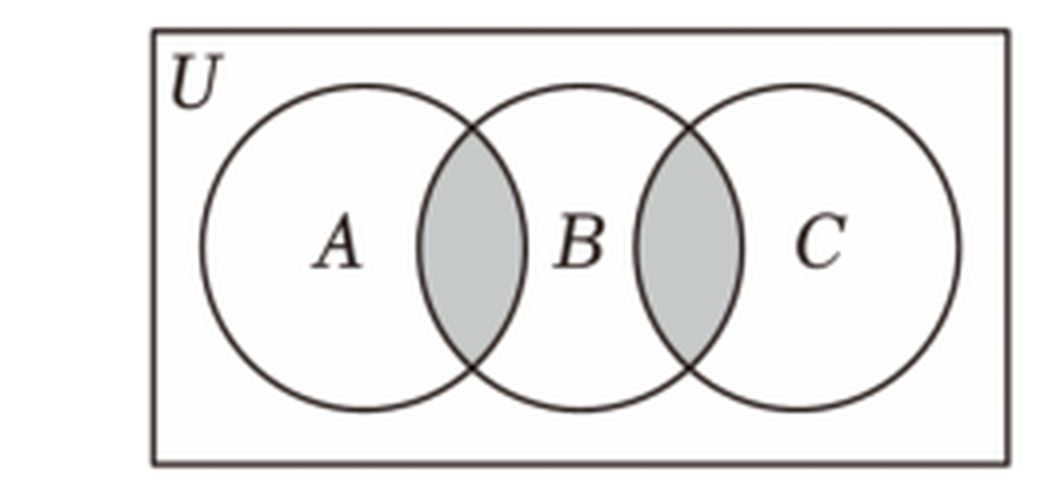
\includegraphics[width=0.30\textwidth]{figures/venn_ABC_lenses.png}
\end{center}

\keepwithprev
A. $B\cap(A\cup C)$\qquad\qquad\qquad B. $B\cap(A\cap C)$

C. $B\cap\complement_U(A\cup C)$\qquad\qquad D. $(A\cup B)\cap(B\cup C)$

\ans{$A$}

\ifanswer
\solbegin
\step{由图中阴影部分得，阴影为集合 $A$、$B$ 的交集和 $B$、$C$ 的交集的并集，}
\step{故阴影部分可表示为 $(A\cap B)\cup(B\cap C)$ 或 $B\cap(A\cup C)$，
故 $A$ 正确. 故选 $A$.}
\solend

\fi

\item 设集合 $P_1=\{x\mid x^2+ax+1>0\}$，$P_2=\{x\mid x^2+ax+2>0\}$，
$Q_1=\{x\mid x^2+x+b>0\}$，$Q_2=\{x\mid x^2+2x+b>0\}$，其中 $a$、$b\in\R$，
对于下列两个命题：①存在 $a$，$P_1$ 不是 $P_2$ 的子集；②存在 $b$ 使得 $Q_1$ 是 $Q_2$
的子集. 下列说法正确的是\mbox{（\quad）}

\keepwithprev
A. ①是真命题，②是假命题\qquad B. ①是假命题，②是真命题

C. ①②都是真命题\qquad\qquad\quad D. ①②都是假命题

\ans{$B$}

\ifanswer
\solbegin
\step{对于集合 $P_1=\{x\mid x^2+ax+1>0\}$，$P_2=\{x\mid x^2+ax+2>0\}$，}
\step{得当 $m\in P_1$ 时，即 $m^2+am+1>0$，得 $m^2+am+2>0$，}
\step{即有 $m\in P_2$，得对任意 $a$，$P_1$ 是 $P_2$ 的子集，故①错误；}
\step{对于集合 $Q_1=\{x\mid x^2+x+b>0\}$，$Q_2=\{x\mid x^2+2x+b>0\}$，}
\step{当 $b=6$ 时，$Q_1=\{x\mid x^2+x+6>0\}=\R$，$Q_2=\{x\mid x^2+2x+6>0\}=\R$，}
\step{得 $Q_1$ 是 $Q_2$ 的子集，所以存在 $b$，使得 $Q_1$ 是 $Q_2$ 的子集，故②正确；}
\step{故选 $B$.}
\solend

\fi

\item 设 $a$、$b\in\R$，则“$a+b>2$ 且 $ab>1$”是“$a>1$ 且 $b>1$”的\mbox{（\quad）}

\keepwithprev
A. 充要条件\qquad\qquad\qquad B. 充分不必要条件

C. 必要不充分条件\qquad\quad D. 既不充分又不必要条件

\ans{$C$}

\ifanswer
\solbegin
\step{因为 $a>1$ 且 $b>1$，所以 $a+b>2$ 且 $ab>1$，}
\step{若已知 $a+b>2$ 且 $ab>1$，可取 $a=\dfrac12$，$b=8$，也满足已知，}
\step{所以“$a+b>2$ 且 $ab>1$”是“$a>1$ 且 $b>1$”的必要不充分条件，故选 $C$.}
\solend

\fi

\item 十七世纪，数学家费马提出猜想：“对任意正整数 $n>2$，关于 $x$、$y$、$z$ 的方程
$x^n+y^n=z^n$ 没有正整数解”. 1995 年数学家安德鲁·怀尔斯发表了完成的证明过程，使它
终成费马大定理. 对费马大定理，若用反证法证明，第一步是假设猜想不成立，即\mbox{（\quad）}

\keepwithprev
A. 对任意正整数 $n>2$，关于 $x$、$y$、$z$ 的方程 $x^n+y^n=z^n$ 都有正整数解

B. 对任意正整数 $n>2$，关于 $x$、$y$、$z$ 的方程 $x^n+y^n=z^n$ 至少存在一组正整数解

C. 存在正整数 $n\leqslant2$，关于 $x$、$y$、$z$ 的方程 $x^n+y^n=z^n$ 至少存在一组正整数解

D. 存在正整数 $n>2$，关于 $x$、$y$、$z$ 的方程 $x^n+y^n=z^n$ 至少存在一组正整数解

\ans{$D$}

\end{enumerate}

\bigsec{三、解答题}

\begin{enumerate}
\setcounter{enumi}{16}

\item 已知 $a$、$b$、$c$ 都是实数，且 $a+b+c=0$，$abc=1$，求证：$a$、$b$、$c$ 中必有一个
大于 $\dfrac32$.

\ifanswer
\solbegin
\step{由 $a+b+c=0$，$abc=1$，得 $a$、$b$、$c$ 中一个正数，两个负数，}
\step{不妨设 $c>0$，由题意得 $a+b=-c,ab=\dfrac1c$，}
\step{由根与系数的关系得 $a$、$b$ 是关于 $x$ 的方程 $x^2+cx+\dfrac1c=0$ 的两个根，}
\step{则 $\Delta=c^2-\dfrac4c=\dfrac{c^3-4}{c}\geqslant0$，}
\step{因为 $c>0$，所以 $c^3\geqslant4$，得 $c\geqslant\sqrt[3]{4}$，}
\step{又 $\dfrac32=\sqrt[3]{\left(\dfrac32\right)^3}=\sqrt[3]{\dfrac{27}{8}}<\sqrt[3]{4}$，}
\step{所以 $c>\dfrac32$，即 $a$、$b$、$c$ 中必有一个大于 $\dfrac32$.}
\solend

\fi

\ansspace[6]

\item 已知关于 $x$ 的一元二次方程 $x^2-mx+4m^2-3=0$ 的两个实根分别为 $x_1,x_2$.

\begin{enumerate}[label=(\arabic*)]
\item $x_1,x_2$ 均为正根，求实数 $m$ 的取值范围；
\item 若 $x_1,x_2$ 满足：$x_1+x_2=x_1x_2$，求实数 $m$ 的值.
\end{enumerate}

\ifanswer
\solbegin
\stepm{(1)}{由 $x_1,x_2$ 均为正根，得}
\step{$\begin{cases}\Delta=(-m)^2-4(4m^2-3)\geqslant0\\ x_1+x_2=m>0\\ x_1\cdot x_2=4m^2-3>0\end{cases}$，}
\step{解得 $\begin{cases}-\dfrac{2\sqrt5}{5}\leqslant m\leqslant\dfrac{2\sqrt5}{5}\\[4pt]
m>0\\[4pt] m\leqslant-\dfrac{\sqrt3}{2}$ 或 $m\geqslant\dfrac{\sqrt3}{2}\end{cases}$，}
\step{即 $\dfrac{\sqrt3}{2}\leqslant m\leqslant\dfrac{2\sqrt5}{5}$；}
\stepm{(2)}{由 (1) 得
$\begin{cases}-\dfrac{2\sqrt5}{5}\leqslant m\leqslant\dfrac{2\sqrt5}{5}\\[4pt]
m=4m^2-3\end{cases}$，解得 $m=1$（舍去）或 $m=-\dfrac34$，}
\step{则 $m=-\dfrac34$.}
\solend

\fi

\ansspace[6]

\item 已知集合 $A=\{x\mid m-1<x<m^2+1\}$，$B=\{x\mid-2<x<2\}$.

\begin{enumerate}[label=(\arabic*)]
\item 当 $m=2$ 时，求 $A\cup B$、$A\cap B$、$\complement_R B$、$A\cap(\complement_R B)$；
\item 若“$x\in A$”是“$x\in B$”成立的必要不充分条件，求实数 $m$ 的取值范围.
\end{enumerate}

\ifanswer
\solbegin
\stepm{(1)}{$m=2$ 时，$A=\{x\mid1<x<5\}$，且 $B=\{x\mid-2<x<2\}$，}
\step{所以 $A\cup B=\{x\mid-2<x<5\}$，$A\cap B=\{x\mid1<x<2\}$，}
\step{$\complement_R B=\{x\mid x\leqslant-2$ 或 $x\geqslant2\}$，
$A\cap(\complement_R B)=\{x\mid2\leqslant x<5\}$；}
\stepm{(2)}{若“$x\in A$”是“$x\in B$”成立的必要不充分条件，则 $B\subset A$，}
\step{所以 $\begin{cases}m-1<-2\\ m^2+1\geqslant2\end{cases}$
或 $\begin{cases}m-1\leqslant-2\\ m^2+1>2\end{cases}$，解得 $m<-1$，}
\step{故 $m$ 的取值范围为 $(-\infty,-1)$.}
\solend

\fi

\ansspace[6]

\item 已知 $m\in\R$，集合 $A=\{x\mid|x-1|\leqslant2\}$，集合
$B=\{x\mid m-3<x\leqslant m+2\}$.

\begin{enumerate}[label=(\arabic*)]
\item 若“$x\in A$”是“$x\in B$”的充分不必要条件，求 $m$ 的取值范围；
\item 若命题“$\forall x\in B$，$x\in\complement_R A$”是真命题，求 $m$ 的取值范围；
\item 若命题“$\exists x\in A$，$x\in B$”是真命题，求 $m$ 的取值范围.
\end{enumerate}

\ifanswer
\solbegin
\stepm{(1)}{集合 $A=\{x\mid|x-1|\leqslant2\}=\{x\mid-1\leqslant x\leqslant3\}$，}
\step{若“$x\in A$”是“$x\in B$”的充分不必要条件，则 $A\subset B$，}
\step{所以 $\begin{cases}m-3<-1\\ 3\leqslant m+2\end{cases}$，解得 $1\leqslant m<2$，}
\step{当 $m=1$ 时，$B=\{x\mid-2<x\leqslant3\}$，符合题意，}
\step{所以 $m$ 的取值范围是 $\{m\mid1\leqslant m<2\}$.}
\stepm{(2)}{若命题“$\forall x\in B$，$x\in\complement_R A$”是真命题，则 $B\subset\complement_R A$，}
\step{又 $\complement_R A=\{x\mid x<-1$ 或 $x>3\}$，$B\neq\varnothing$，
所以 $m+2<-1$ 或 $m-3\geqslant3$，}
\step{解得 $m<-3$ 或 $m\geqslant6$，所以 $\{m\mid m<-3$ 或 $m\geqslant6\}$；}
\stepm{(3)}{因为 $\exists x\in A$，$x\in B$ 是真命题，所以 $A\cap B\neq\varnothing$，}
\step{当 $A\cap B=\varnothing$ 时，所以 $m+2<-1$ 或 $m-3\geqslant3$，
即 $m<-3$ 或 $m\geqslant6$，}
\step{所以当 $A\cap B\neq\varnothing$ 时，$m$ 的取值范围是 $\{m\mid-3\leqslant m<6\}$，}
\step{则 $m$ 的取值范围是 $\{m\mid-3\leqslant m<6\}$.}
\solend

\fi

\ansspace[6]

\item 对于函数 $f(x)$，若 $f(x_0)=x_0$，则称 $x_0$ 为 $f(x)$ 的“不动点”；若
$f[f(x_0)]=x_0$，则称 $x_0$ 为 $f(x)$ 的“稳定点”. 函数 $f(x)$ 的“不动点”和“稳定点”
的集合分别记为 $A$ 和 $B$，即 $A=\{x\mid f(x)=x\}$，$B=\{x\mid f[f(x)]=x\}$.

\begin{enumerate}[label=(\arabic*)]
\item 设函数 $f(x)=3x+4$，求集合 $A$ 和 $B$；
\item 求证：$A\sub B$；
\item 设函数 $f(x)=ax^2+bx+c(a\neq0)$，且 $A=\varnothing$，求证：$B=\varnothing$.
\end{enumerate}

\ifanswer
\solbegin
\stepm{(1)}{令 $f(x)=3x+4=x$，解得 $x=-2$，故有 $A=\{-2\}$，}
\step{由于 $f[f(x)]=3(3x+4)+4=9x+16$，}
\step{令 $9x+16=x$，得 $x=-2$，故有 $B=\{-2\}$；}
\stepm{(2)}{若 $A=\varnothing$，则 $A\sub B$ 显然成立；}
\step{若 $A\neq\varnothing$，设 $t\in A$，则 $f(t)=t$，$f(f(t))=f(t)=t$，}
\step{所以 $t\in B$，故 $A\sub B$.}
\stepm{(3)}{因为 $A=\{x\mid f(x)=x\}=\varnothing$，所以 $ax^2+bx+c=x$ 无解，}
\step{即 $\Delta=(b-1)^2-4a<0$，}
\step{①当 $a>0$ 时，二次函数 $y=f(x)-x$，}
\step{即 $y=ax^2+(b-1)x+c$ 的图象在 $x$ 轴的上方，}
\step{所以 $\forall x\in\R$，$f(x)-x>0$ 恒成立，所以 $\forall x\in\R$，
$f(x)>x$ 恒成立，}
\step{所以 $\forall x\in\R$，$f[f(x)]>f(x)>x$ 恒成立，即 $B=\varnothing$；}
\step{②当 $a<0$ 时，同理可证 $B=\varnothing$；}
\step{综上，对于函数 $f(x)=ax^2+bx+c(a\neq0)$，当 $A=\varnothing$ 时，$B=\varnothing$.}
\solend

\fi

\ansspace*[10]

\end{enumerate}

\end{document}
"
%
% 原始材料是微信公众号图文（公众号「魔都数学加油站」连载「27学年高一 26」，2026-09-21 发布，
% 原文标题「27学年高一26——2026-2027年上海市交附闵行高一上周练2」），
% 正文为 10 张 PNG 页（1080×1527，各页同尺寸）。原文本身就是一份**讲评版**——
% 题目下方直接印出【解析】（本卷无单独的【答案】行，填空题答案都写在解析里）。
% 试题文字与解析均照原卷录入，未改内容。卷面的粉色斜水印「魔都数学加油站」属水印，未录入。
%
% 卷首标题：原卷印作「2026-2027 年交附闵行高一上周练 2」（公众号标题里的「上海市」
% 三字卷面标题行没有，本稿照卷面），年份区间按全稿惯例排 en dash，前缀照原卷保留「年」。
%
% 与原卷的排版差异（均已在 README「说明」中交代）：
%   ① 原文自**第 3 题**起（第 1、2 题未在该文中发布），故本稿题号亦自 3 起；
%   ② 原卷本就印有「一、填空题」「二、选择题」「三、解答题」三节标题，本稿照原卷分节，
%      只把标题改排成全稿统一的「大节标题」样式；
%   ③ 原卷第 16 题的答案「D」直接印在题干末尾的括号内（原卷把括号连同 D 单独占一行），
%      第 13—15 题的括号空着、答案写在解析末句「故选 A／B／C」里；填空题的答案也都嵌在
%      解析里，本稿统一改为试卷版隐去、答案版以 \ans{} 给出（选择题另附【解析】）；
%   ④ 子集符号原卷两种并用：第 4 题题干与第 8 题、第 21(2) 题等作带下划线的 $\subseteq$，
%      第 19(2)、20(1)(2) 题作真包含的 $\subset$，本稿分别照录为 $\sub$ 与 $\subset$；
%   ⑤ 补集符号原卷作 $\complement_R$、$\complement_U$（第 4 题命题④、第 13 题选项 C、
%      第 19—20 题），本稿照录；
%   ⑥ 原卷的实数集 R 一律作斜体（第 11 题「$a\in R$」、第 14 题「$a$、$b\in R$」与解析的
%      $\{x\mid x^2+x+6>0\}=R$ 等），本稿按全稿惯例统一写作 $\R$；
%   ⑦ 原卷填空的横线约两个字宽，本稿按全稿惯例统一排 \blankline[4.4em]；
%   ⑧ 原卷未印副标题，本稿按全稿惯例补出副标题「集合与常用逻辑用语」；
%   ⑨ 第 13 题的 Venn 图原卷印在题干右侧（第 5 页），本稿移至题干之后；
%      图取原卷截图、4× LANCZOS 放大（figures/venn_ABC_lenses.png，
%      阴影为 $A\cap B$ 与 $B\cap C$ 两个交带，即 $(A\cap B)\cup(B\cap C)$）。
%
% 原卷存疑一处（照抄原卷、未改，见源码中该处上方注释）：
%   ① 第 12 题【解析】首步的方程组里印 $t<2$，而其后三处与末行答案都作 $t\leqslant2$
%      （$\left[\dfrac85,\dfrac{17}{10}\right)\cup\left(\dfrac95,2\right]$ 含 $2$）——
%      按题意 $N=\left\{x\mid t-\dfrac35\leqslant x\leqslant t\right\}\sub\{x\mid1\leqslant x\leqslant2\}$
%      只要求 $t\leqslant2$（$t=2$ 时 $N=\left[\dfrac75,2\right]$ 确实含于其中），
%      故方程组里的 $t<2$ 应是原卷笔误；本稿两处都照原卷录入、未互相迁就。
% 另：第 20(3) 题解析末两行原卷即作同话重复，照原卷录入。

\documentclass[a4paper,11pt]{article}
\usepackage{common}

\begin{document}

\examtitlest[3]{2026--2027 年交附闵行高一上周练 2}{集合与常用逻辑用语}

\bigsec{一、填空题}

\begin{enumerate}
\setcounter{enumi}{2}

\item 命题甲：集合 $M=\{x\mid kx^2-2kx+1=0\}$ 为空集；命题乙：关于 $x$ 的不等式
$x^2+(k-1)x+4>0$ 的解集为 $\R$. 若命题甲、乙中有且只有一个是真命题，则实数 $k$ 的取
值范围是 \blankline[4.4em].

\ifanswer
\solbegin
\step{因为集合 $M=\{x\mid kx^2-2kx+1=0\}$ 为空集，}
\step{当 $k\neq0$ 时，$\Delta=(-2k)^2-4k<0$，解得 $0<k<1$，}
\step{当 $k=0$ 时，方程变为 $1=0$，无解，满足题意，故 $0\leqslant k<1$；}
\step{又关于 $x$ 的不等式 $x^2+(k-1)x+4>0$ 的解集为 $\R$，}
\step{所以 $\Delta'=(k-1)^2-4\times4<0$，解得 $-3<k<5$，}
\step{当甲命题为真，乙命题为假时，无解，}
\step{当甲命题为假，乙命题为真时，$k\in(-3,0)\cup[1,5)$.}
\solend

\fi

\item 对任意 $A$、$B\sub\R$，记 $A\oplus B=\{x\mid x\in A\cup B,x\notin A\cap B\}$，
并称 $A\oplus B$ 为集合 $A$、$B$ 的对称差. 例如：若 $A=\{1,2,3\},B=\{2,3,4\}$，
则 $A\oplus B=\{1,4\}$. 下列命题中，为真命题的是 \blankline[4.4em].

\keepwithprev
①若 $A$、$B\sub\R$ 且 $A\oplus B\sub A$，则 $A\sub B$

②若 $A$、$B\sub\R$ 且 $A\oplus B=\varnothing$，则 $A=B$

③若 $A$、$B\sub\R$ 且 $A\oplus B=B$，则 $A=\varnothing$

④对任意 $A$、$B\sub\R$，都有 $A\oplus B=\complement_R A\oplus\complement_R B$

\ans{②③④}

\ifanswer
\solbegin
\step{对于①，因为 $A\oplus B\sub A$，
所以 $\{x\mid x\in A\cup B,x\notin A\cap B\}\sub A$，}
\step{故 $B\sub A$，①错误；}
\step{对于②，$A$、$B\sub\R$ 且 $A\oplus B=\varnothing$，
则 $\varnothing=\{x\mid x\in A\cup B,x\notin A\cap B\}$，}
\step{即 $A\cup B=A\cap B$，所以 $A=B$，②正确；}
\step{对于③，$A$、$B\sub\R$ 且 $A\oplus B=B$，
则 $B=\{x\mid x\in A\cup B,x\notin A\cap B\}$，}
\step{故 $A\sub B$，且 $B$ 中元素不在 $A\cap B$ 中，故 $A=\varnothing$，③正确；}
\step{对于④，$\complement_R A\oplus\complement_R B
=\{x\mid x\in\complement_R A\cup\complement_R B,x\notin\complement_R A\cap\complement_R B\}$，}
\step{其中 $\complement_R A\cup\complement_R B=\complement_R(A\cap B)$，
$\complement_R A\cap\complement_R B=\complement_R(A\cup B)$，}
\step{故 $\complement_R A\oplus\complement_R B
=\{x\mid x\in\complement_R(A\cap B),x\notin\complement_R(A\cup B)\}
=\{x\mid x\in A\cup B,x\notin A\cap B\}$，}
\step{而 $A\oplus B=\{x\mid x\in A\cup B,x\notin A\cap B\}$，
故 $A\oplus B=\complement_R A\oplus\complement_R B$，④正确.}
\step{故正确的是②③④.}
\solend

\fi

\item 已知 $A=\{a_1,a_2,a_3,a_4\},B=\{a^2\mid a\in A\}$，其中 $a_1<a_2<a_3<a_4$，
且 $a_1$、$a_2$、$a_3$、$a_4$ 均为整数，若 $A\cap B=\{a_3,a_4\},a_1+a_3=0$，
且 $A\cup B$ 中的所有元素之和为 $270$，则集合 $A$ 中所有元素之和为 \blankline[4.4em].

\ifanswer
\solbegin
\step{$A=\{a_1,a_2,a_3,a_4\},B=\{a^2\mid a\in A\}$，
因为 $A\cap B=\{a_3,a_4\},a_1+a_3=0$，}
\step{所以 $A=\{a_1,a_2,a_3,a_4\},B=\left\{a_1^2,a_2^2,a_4^2\right\}$，}
\step{若 $a_1^2=a_3$，则 $a_1=-1,a_3=1$，则 $a_2=0$，
此时 $A=\{-1,0,1,a_4\},B=\{0,1,a_4^2\}$，}
\step{因为 $A\cup B$ 中的所有元素之和为 $270$，
所以 $-1+0+1+a_4+1+a_4^2=270$，}
\step{无正整数解，舍去；}
\step{若 $a_2^2=a_3$，① $a_4^2=a_4$，所以 $a_4=1$，矛盾；}
\step{② $a_1^2=a_4$，此时 $A\cup B=\left\{-a_2^2,a_2,a_2^2,a_1^2,a_4^2\right\}$，
所以 $a_2^8+a_2^4+a_2=270$，}
\step{所以 $a_2=-2$，此时 $a_1=-4,a_2=-2,a_3=4,a_4=16$；}
\step{若 $a_4^2=a_3$，显然不成立；}
\step{综上，集合 $A$ 中所有元素之和为 $-4-2+4+16=14$.}
\solend

\fi

\item 将集合 $M=\{a_1,a_2,a_3,\cdots,a_n\}$ 分拆成两个集合 $A_i$ 和 $B_j$，且
$M\supseteq A_i\cup B_j$，$A_i\cap B_j=\varnothing$，这样的分拆方法共有 \blankline[4.4em] 种.

\ifanswer
\solbegin
\step{按集合 $A_i$ 中的元素个数进行分类：}
\step{若 $A_i$ 中有 $0$ 个元素（即 $C_n^0$ 种）时，则 $B_j$ 有 $2^n$ 种，
共有 $2^nC_n^0$ 种；}
\step{若 $A_i$ 中有 $1$ 个元素（即 $C_n^1$ 种）时，则 $B_j$ 有 $2^{n-1}$ 种，
共有 $2^{n-1}C_n^1$ 种；}
\step{若 $A_i$ 中有 $2$ 个元素（即 $C_n^2$ 种）时，则 $B_j$ 有 $2^{n-2}$ 种，
共有 $2^{n-2}C_n^2$ 种；}
\step{若 $A_i$ 中有 $3$ 个元素（即 $C_n^3$ 种）时，则 $B_j$ 有 $2^{n-3}$ 种，
共有 $2^{n-3}C_n^3$ 种；}
\step{若 $A_i$ 中有 $n$ 个元素（即 $C_n^n$ 种）时，则 $B_j$ 有 $2^0$ 种，
共有 $2^0C_n^n$ 种；}
\step{得 $2^nC_n^0+2^{n-1}C_n^1+2^{n-2}C_n^2+\cdots+2^0C_n^n=(1+2)^n$，
故这样的分拆方法有 $3^n$ 种.}
\solend

\fi

\item 已知集合 $A=\{x\mid x<2,x\in\Z\}$，$B=\{x\mid x>0,x\in\Z\}$，则
$A\cap B=$ \blankline[4.4em].

\ifanswer
\solbegin
\step{因为 $A=\{x\mid x<2,x\in\Z\}$，$B=\{x\mid x>0,x\in\Z\}$，}
\step{所以 $A\cap B=\{x\mid0<x<2,x\in\Z\}=\{1\}$.}
\solend

\fi

\item 已知集合 $A=\{x\mid(a-1)x^2+3x-2=0\}$，$B=\{x\mid x^2-3x+2=0\}$，若
$A\sub B$，求实数 $a$ 的取值范围是 \blankline[4.4em].

\ifanswer
\solbegin
\step{由方程 $x^2-3x+2=0$，解得 $x=1$ 或 $x=2$，即 $B=\{1,2\}$，}
\step{因为 $A\sub B$，所以 $A=\varnothing$ 或 $A=\{1\}$ 或 $A=\{2\}$ 或 $A=\{1,2\}$，}
\step{当 $A=\varnothing$ 时，
则 $\begin{cases}a\neq1\\ \Delta=3^2-4(a-1)\times(-2)<0\end{cases}$，
解得 $a<-\dfrac18$；}
\step{将 $x=1$ 代入方程 $(a-1)x^2+3x-2=0$，得 $a=0$，}
\step{此时 $A=\{x\mid-x^2+3x-2=0\}=\{1,2\}$，满足条件；}
\step{将 $x=2$ 代入方程 $(a-1)x^2+3x-2=0$，得到 $a=0$，上面已经验证满足条件；}
\step{综上所述，$a$ 的取值范围是 $\left(-\infty,-\dfrac18\right)\cup\{0\}$.}
\solend

\fi

\item 已知方程 $x^2-3x+a=0$ 的两根都大于 $1$，则 $a$ 的取值范围为 \blankline[4.4em].

\ifanswer
\solbegin
\step{由题意得 $\Delta=9-4a\geqslant0$，$x_1+x_2=3$，$x_1x_2=a$，
所以 $a\leqslant\dfrac94$，}
\step{则 $(x_1-1)(x_2-1)=x_1x_2-(x_1+x_2)+1=a-3+1>0$，所以 $a>2$，}
\step{故 $a$ 的范围为 $\left(2,\dfrac94\right]$.}
\solend

\fi

\item 设 $x_1$、$x_2$ 是方程 $x^2+x-3=0$ 的两个实数根，则 $x_1^2-x_2+2024=$
\blankline[4.4em].

\ifanswer
\solbegin
\step{由题意得 $x_1^2=3-x_1$，$x_1+x_2=-1$，}
\step{则 $x_1^2-x_2+2024=3-x_1-x_2+2024=2027-(-1)=2028$.}
\solend

\fi

\item 已知 $a\in\R$，若关于 $x$ 的方程 $x^2+ax+a^2-8=0$ 有两个实根 $x_1$、$x_2$，且
$\dfrac1{x_1}+\dfrac1{x_2}=-\dfrac12$，则 $a$ 的值为 \blankline[4.4em].

\ifanswer
\solbegin
\step{由题意得 $\Delta=a^2-4(a^2-8)=32-3a^2\geqslant0$，
解得 $a^2\leqslant\dfrac{32}{3}$，}
\step{由韦达定理得 $x_1+x_2=-a$，$x_1x_2=a^2-8$，}
\step{则 $\dfrac1{x_1}+\dfrac1{x_2}=\dfrac{x_1+x_2}{x_1x_2}
=\dfrac{-a}{a^2-8}=-\dfrac12$，}
\step{即 $a^2-2a-8=(a-4)(a+2)=0$，解得 $a=4$ 或 $a=-2$.}
\step{又 $a^2\leqslant\dfrac{32}{3}$，则 $a=-2$.}
\solend

\fi

\item 定义集合 $P=\{x\mid a\leqslant x\leqslant b\}$ 的“长度”是 $b-a$，其中 $a$、
$b\in\R$. 已知集合 $M=\left\{x\mid\dfrac65\leqslant x\leqslant\dfrac{17}{10}\right\}$，
$N=\left\{x\mid t-\dfrac35\leqslant x\leqslant t\right\}$，且 $M$、$N$ 都是集合
$\{x\mid1\leqslant x\leqslant2\}$ 的子集，若集合 $M\cup N$ 的“长度”大于 $\dfrac35$，
则 $t$ 的取值范围是 \blankline[4.4em].

\ifanswer
\solbegin
\step{因为 $N=\left\{x\mid t-\dfrac35\leqslant x\leqslant t\right\}$
是集合 $\{x\mid1\leqslant x\leqslant2\}$ 的子集，}
% 注：下一行方程组里的 $t<2$ 系原卷所印（本稿照录），与其后三处及末行答案的
%     $t\leqslant2$ 自相矛盾——按题意应为 $t\leqslant2$，见文件头「原卷存疑」①。
\step{所以 $\begin{cases}t-\dfrac35\geqslant1\\[2pt] t<2\end{cases}$，
解得 $\dfrac85\leqslant t\leqslant2$，}
\step{又 $M=\left\{x\mid\dfrac65\leqslant x\leqslant\dfrac{17}{10}\right\}$，
得集合 $M$ 的“长度”为 $\dfrac{17}{10}-\dfrac65=\dfrac12$，}
\step{又 $N=\left\{x\mid t-\dfrac35\leqslant x\leqslant t\right\}$，
要使集合 $M\cup N$ 的“长度”大于 $\dfrac35$，}
\step{若 $M\cup N=\left\{x\mid t-\dfrac35\leqslant x\leqslant\dfrac{17}{10}\right\}$，
则 $\dfrac{17}{10}-t+\dfrac35>\dfrac35$，所以 $t<\dfrac{17}{10}$，}
\step{又 $\dfrac85\leqslant t\leqslant2$，所以 $\dfrac85\leqslant t<\dfrac{17}{10}$；}
\step{若 $M\cup N=\left\{x\mid\dfrac65\leqslant x\leqslant t\right\}$，
则 $t-\dfrac65>\dfrac35$，所以 $t>\dfrac95$，}
\step{又 $\dfrac85\leqslant t\leqslant2$，所以 $\dfrac95<t\leqslant2$；}
\step{则 $t$ 的取值范围是 $\left[\dfrac85,\dfrac{17}{10}\right)\cup\left(\dfrac95,2\right]$.}
\solend

\fi

\end{enumerate}

% 第 13 题是「题干 + 图 + 选项」约 5.7cm 的一整块（图 0.30\textwidth、宽高比 0.477 → 高 2.29cm，
% 加题干 1 行、选项 2 行与段间距）。`\keepwithprev` 只挡得住「题干—选项」之间，挡不住
% 夹在中间的图——实测断点落在题干之后，题干孤零零留在 p1、图与四个选项整页翻到 p2
% （切页审计的 A 类）。故照 高一30 第 4 题的成例先量一次页高；**守卫要放在 `\bigsec` 之前**
% 连节标题一起量（放标题之后会把「二、选择题」孤立在页末，正是 高一40 修过的那类 B 类）。
% 7cm ＝ 节标题约 1.1cm ＋ 第 13 题那块约 5.7cm（留少量余量）。
\needvspace{7cm}
\bigsec{二、选择题}

\begin{enumerate}
\setcounter{enumi}{12}

\item 图中阴影部分用集合符号可以表示为\mbox{（\quad）}

\begin{center}
% 图取原卷截图、4× LANCZOS 放大（原卷把图印在题干右侧，本稿移至此处，见文件头⑨）。
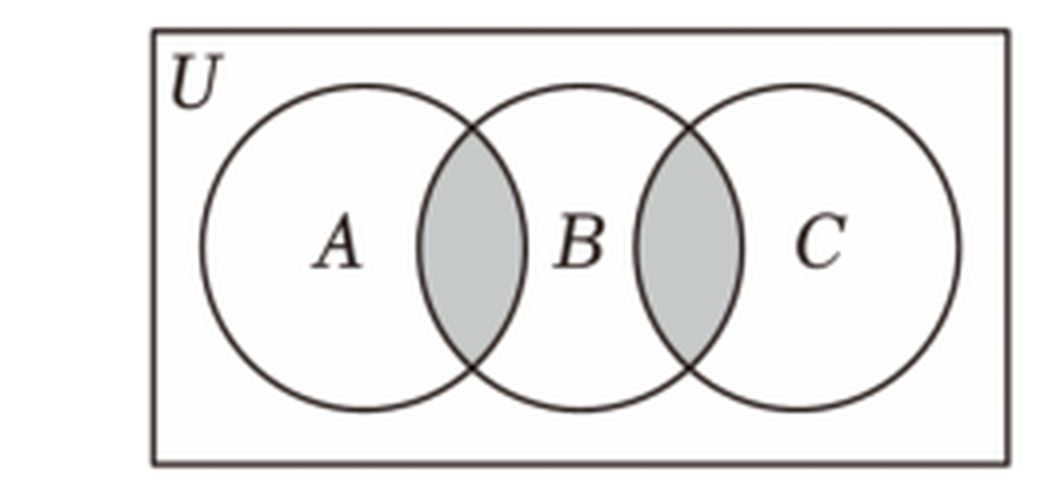
\includegraphics[width=0.30\textwidth]{figures/venn_ABC_lenses.png}
\end{center}

\keepwithprev
A. $B\cap(A\cup C)$\qquad\qquad\qquad B. $B\cap(A\cap C)$

C. $B\cap\complement_U(A\cup C)$\qquad\qquad D. $(A\cup B)\cap(B\cup C)$

\ans{$A$}

\ifanswer
\solbegin
\step{由图中阴影部分得，阴影为集合 $A$、$B$ 的交集和 $B$、$C$ 的交集的并集，}
\step{故阴影部分可表示为 $(A\cap B)\cup(B\cap C)$ 或 $B\cap(A\cup C)$，
故 $A$ 正确. 故选 $A$.}
\solend

\fi

\item 设集合 $P_1=\{x\mid x^2+ax+1>0\}$，$P_2=\{x\mid x^2+ax+2>0\}$，
$Q_1=\{x\mid x^2+x+b>0\}$，$Q_2=\{x\mid x^2+2x+b>0\}$，其中 $a$、$b\in\R$，
对于下列两个命题：①存在 $a$，$P_1$ 不是 $P_2$ 的子集；②存在 $b$ 使得 $Q_1$ 是 $Q_2$
的子集. 下列说法正确的是\mbox{（\quad）}

\keepwithprev
A. ①是真命题，②是假命题\qquad B. ①是假命题，②是真命题

C. ①②都是真命题\qquad\qquad\quad D. ①②都是假命题

\ans{$B$}

\ifanswer
\solbegin
\step{对于集合 $P_1=\{x\mid x^2+ax+1>0\}$，$P_2=\{x\mid x^2+ax+2>0\}$，}
\step{得当 $m\in P_1$ 时，即 $m^2+am+1>0$，得 $m^2+am+2>0$，}
\step{即有 $m\in P_2$，得对任意 $a$，$P_1$ 是 $P_2$ 的子集，故①错误；}
\step{对于集合 $Q_1=\{x\mid x^2+x+b>0\}$，$Q_2=\{x\mid x^2+2x+b>0\}$，}
\step{当 $b=6$ 时，$Q_1=\{x\mid x^2+x+6>0\}=\R$，$Q_2=\{x\mid x^2+2x+6>0\}=\R$，}
\step{得 $Q_1$ 是 $Q_2$ 的子集，所以存在 $b$，使得 $Q_1$ 是 $Q_2$ 的子集，故②正确；}
\step{故选 $B$.}
\solend

\fi

\item 设 $a$、$b\in\R$，则“$a+b>2$ 且 $ab>1$”是“$a>1$ 且 $b>1$”的\mbox{（\quad）}

\keepwithprev
A. 充要条件\qquad\qquad\qquad B. 充分不必要条件

C. 必要不充分条件\qquad\quad D. 既不充分又不必要条件

\ans{$C$}

\ifanswer
\solbegin
\step{因为 $a>1$ 且 $b>1$，所以 $a+b>2$ 且 $ab>1$，}
\step{若已知 $a+b>2$ 且 $ab>1$，可取 $a=\dfrac12$，$b=8$，也满足已知，}
\step{所以“$a+b>2$ 且 $ab>1$”是“$a>1$ 且 $b>1$”的必要不充分条件，故选 $C$.}
\solend

\fi

\item 十七世纪，数学家费马提出猜想：“对任意正整数 $n>2$，关于 $x$、$y$、$z$ 的方程
$x^n+y^n=z^n$ 没有正整数解”. 1995 年数学家安德鲁·怀尔斯发表了完成的证明过程，使它
终成费马大定理. 对费马大定理，若用反证法证明，第一步是假设猜想不成立，即\mbox{（\quad）}

\keepwithprev
A. 对任意正整数 $n>2$，关于 $x$、$y$、$z$ 的方程 $x^n+y^n=z^n$ 都有正整数解

B. 对任意正整数 $n>2$，关于 $x$、$y$、$z$ 的方程 $x^n+y^n=z^n$ 至少存在一组正整数解

C. 存在正整数 $n\leqslant2$，关于 $x$、$y$、$z$ 的方程 $x^n+y^n=z^n$ 至少存在一组正整数解

D. 存在正整数 $n>2$，关于 $x$、$y$、$z$ 的方程 $x^n+y^n=z^n$ 至少存在一组正整数解

\ans{$D$}

\end{enumerate}

\bigsec{三、解答题}

\begin{enumerate}
\setcounter{enumi}{16}

\item 已知 $a$、$b$、$c$ 都是实数，且 $a+b+c=0$，$abc=1$，求证：$a$、$b$、$c$ 中必有一个
大于 $\dfrac32$.

\ifanswer
\solbegin
\step{由 $a+b+c=0$，$abc=1$，得 $a$、$b$、$c$ 中一个正数，两个负数，}
\step{不妨设 $c>0$，由题意得 $a+b=-c,ab=\dfrac1c$，}
\step{由根与系数的关系得 $a$、$b$ 是关于 $x$ 的方程 $x^2+cx+\dfrac1c=0$ 的两个根，}
\step{则 $\Delta=c^2-\dfrac4c=\dfrac{c^3-4}{c}\geqslant0$，}
\step{因为 $c>0$，所以 $c^3\geqslant4$，得 $c\geqslant\sqrt[3]{4}$，}
\step{又 $\dfrac32=\sqrt[3]{\left(\dfrac32\right)^3}=\sqrt[3]{\dfrac{27}{8}}<\sqrt[3]{4}$，}
\step{所以 $c>\dfrac32$，即 $a$、$b$、$c$ 中必有一个大于 $\dfrac32$.}
\solend

\fi

\ansspace[6]

\item 已知关于 $x$ 的一元二次方程 $x^2-mx+4m^2-3=0$ 的两个实根分别为 $x_1,x_2$.

\begin{enumerate}[label=(\arabic*)]
\item $x_1,x_2$ 均为正根，求实数 $m$ 的取值范围；
\item 若 $x_1,x_2$ 满足：$x_1+x_2=x_1x_2$，求实数 $m$ 的值.
\end{enumerate}

\ifanswer
\solbegin
\stepm{(1)}{由 $x_1,x_2$ 均为正根，得}
\step{$\begin{cases}\Delta=(-m)^2-4(4m^2-3)\geqslant0\\ x_1+x_2=m>0\\ x_1\cdot x_2=4m^2-3>0\end{cases}$，}
\step{解得 $\begin{cases}-\dfrac{2\sqrt5}{5}\leqslant m\leqslant\dfrac{2\sqrt5}{5}\\[4pt]
m>0\\[4pt] m\leqslant-\dfrac{\sqrt3}{2}$ 或 $m\geqslant\dfrac{\sqrt3}{2}\end{cases}$，}
\step{即 $\dfrac{\sqrt3}{2}\leqslant m\leqslant\dfrac{2\sqrt5}{5}$；}
\stepm{(2)}{由 (1) 得
$\begin{cases}-\dfrac{2\sqrt5}{5}\leqslant m\leqslant\dfrac{2\sqrt5}{5}\\[4pt]
m=4m^2-3\end{cases}$，解得 $m=1$（舍去）或 $m=-\dfrac34$，}
\step{则 $m=-\dfrac34$.}
\solend

\fi

\ansspace[6]

\item 已知集合 $A=\{x\mid m-1<x<m^2+1\}$，$B=\{x\mid-2<x<2\}$.

\begin{enumerate}[label=(\arabic*)]
\item 当 $m=2$ 时，求 $A\cup B$、$A\cap B$、$\complement_R B$、$A\cap(\complement_R B)$；
\item 若“$x\in A$”是“$x\in B$”成立的必要不充分条件，求实数 $m$ 的取值范围.
\end{enumerate}

\ifanswer
\solbegin
\stepm{(1)}{$m=2$ 时，$A=\{x\mid1<x<5\}$，且 $B=\{x\mid-2<x<2\}$，}
\step{所以 $A\cup B=\{x\mid-2<x<5\}$，$A\cap B=\{x\mid1<x<2\}$，}
\step{$\complement_R B=\{x\mid x\leqslant-2$ 或 $x\geqslant2\}$，
$A\cap(\complement_R B)=\{x\mid2\leqslant x<5\}$；}
\stepm{(2)}{若“$x\in A$”是“$x\in B$”成立的必要不充分条件，则 $B\subset A$，}
\step{所以 $\begin{cases}m-1<-2\\ m^2+1\geqslant2\end{cases}$
或 $\begin{cases}m-1\leqslant-2\\ m^2+1>2\end{cases}$，解得 $m<-1$，}
\step{故 $m$ 的取值范围为 $(-\infty,-1)$.}
\solend

\fi

\ansspace[6]

\item 已知 $m\in\R$，集合 $A=\{x\mid|x-1|\leqslant2\}$，集合
$B=\{x\mid m-3<x\leqslant m+2\}$.

\begin{enumerate}[label=(\arabic*)]
\item 若“$x\in A$”是“$x\in B$”的充分不必要条件，求 $m$ 的取值范围；
\item 若命题“$\forall x\in B$，$x\in\complement_R A$”是真命题，求 $m$ 的取值范围；
\item 若命题“$\exists x\in A$，$x\in B$”是真命题，求 $m$ 的取值范围.
\end{enumerate}

\ifanswer
\solbegin
\stepm{(1)}{集合 $A=\{x\mid|x-1|\leqslant2\}=\{x\mid-1\leqslant x\leqslant3\}$，}
\step{若“$x\in A$”是“$x\in B$”的充分不必要条件，则 $A\subset B$，}
\step{所以 $\begin{cases}m-3<-1\\ 3\leqslant m+2\end{cases}$，解得 $1\leqslant m<2$，}
\step{当 $m=1$ 时，$B=\{x\mid-2<x\leqslant3\}$，符合题意，}
\step{所以 $m$ 的取值范围是 $\{m\mid1\leqslant m<2\}$.}
\stepm{(2)}{若命题“$\forall x\in B$，$x\in\complement_R A$”是真命题，则 $B\subset\complement_R A$，}
\step{又 $\complement_R A=\{x\mid x<-1$ 或 $x>3\}$，$B\neq\varnothing$，
所以 $m+2<-1$ 或 $m-3\geqslant3$，}
\step{解得 $m<-3$ 或 $m\geqslant6$，所以 $\{m\mid m<-3$ 或 $m\geqslant6\}$；}
\stepm{(3)}{因为 $\exists x\in A$，$x\in B$ 是真命题，所以 $A\cap B\neq\varnothing$，}
\step{当 $A\cap B=\varnothing$ 时，所以 $m+2<-1$ 或 $m-3\geqslant3$，
即 $m<-3$ 或 $m\geqslant6$，}
\step{所以当 $A\cap B\neq\varnothing$ 时，$m$ 的取值范围是 $\{m\mid-3\leqslant m<6\}$，}
\step{则 $m$ 的取值范围是 $\{m\mid-3\leqslant m<6\}$.}
\solend

\fi

\ansspace[6]

\item 对于函数 $f(x)$，若 $f(x_0)=x_0$，则称 $x_0$ 为 $f(x)$ 的“不动点”；若
$f[f(x_0)]=x_0$，则称 $x_0$ 为 $f(x)$ 的“稳定点”. 函数 $f(x)$ 的“不动点”和“稳定点”
的集合分别记为 $A$ 和 $B$，即 $A=\{x\mid f(x)=x\}$，$B=\{x\mid f[f(x)]=x\}$.

\begin{enumerate}[label=(\arabic*)]
\item 设函数 $f(x)=3x+4$，求集合 $A$ 和 $B$；
\item 求证：$A\sub B$；
\item 设函数 $f(x)=ax^2+bx+c(a\neq0)$，且 $A=\varnothing$，求证：$B=\varnothing$.
\end{enumerate}

\ifanswer
\solbegin
\stepm{(1)}{令 $f(x)=3x+4=x$，解得 $x=-2$，故有 $A=\{-2\}$，}
\step{由于 $f[f(x)]=3(3x+4)+4=9x+16$，}
\step{令 $9x+16=x$，得 $x=-2$，故有 $B=\{-2\}$；}
\stepm{(2)}{若 $A=\varnothing$，则 $A\sub B$ 显然成立；}
\step{若 $A\neq\varnothing$，设 $t\in A$，则 $f(t)=t$，$f(f(t))=f(t)=t$，}
\step{所以 $t\in B$，故 $A\sub B$.}
\stepm{(3)}{因为 $A=\{x\mid f(x)=x\}=\varnothing$，所以 $ax^2+bx+c=x$ 无解，}
\step{即 $\Delta=(b-1)^2-4a<0$，}
\step{①当 $a>0$ 时，二次函数 $y=f(x)-x$，}
\step{即 $y=ax^2+(b-1)x+c$ 的图象在 $x$ 轴的上方，}
\step{所以 $\forall x\in\R$，$f(x)-x>0$ 恒成立，所以 $\forall x\in\R$，
$f(x)>x$ 恒成立，}
\step{所以 $\forall x\in\R$，$f[f(x)]>f(x)>x$ 恒成立，即 $B=\varnothing$；}
\step{②当 $a<0$ 时，同理可证 $B=\varnothing$；}
\step{综上，对于函数 $f(x)=ax^2+bx+c(a\neq0)$，当 $A=\varnothing$ 时，$B=\varnothing$.}
\solend

\fi

\ansspace*[10]

\end{enumerate}

\end{document}
"
% 紧凑版：xelatex "\def\iscompact{1}% 高一26_交附闵行_周练2.tex
%   —— 高一上数学「2026-2027 年交附闵行高一上周练 2」（试卷版/答案版）
% 试卷版：xelatex 高一26_交附闵行_周练2.tex
% 答案版：xelatex "\def\isanswer{1}% 高一26_交附闵行_周练2.tex
%   —— 高一上数学「2026-2027 年交附闵行高一上周练 2」（试卷版/答案版）
% 试卷版：xelatex 高一26_交附闵行_周练2.tex
% 答案版：xelatex "\def\isanswer{1}% 高一26_交附闵行_周练2.tex
%   —— 高一上数学「2026-2027 年交附闵行高一上周练 2」（试卷版/答案版）
% 试卷版：xelatex 高一26_交附闵行_周练2.tex
% 答案版：xelatex "\def\isanswer{1}\input{高一26_交附闵行_周练2.tex}"
% 紧凑版：xelatex "\def\iscompact{1}\input{高一26_交附闵行_周练2.tex}"
%
% 原始材料是微信公众号图文（公众号「魔都数学加油站」连载「27学年高一 26」，2026-09-21 发布，
% 原文标题「27学年高一26——2026-2027年上海市交附闵行高一上周练2」），
% 正文为 10 张 PNG 页（1080×1527，各页同尺寸）。原文本身就是一份**讲评版**——
% 题目下方直接印出【解析】（本卷无单独的【答案】行，填空题答案都写在解析里）。
% 试题文字与解析均照原卷录入，未改内容。卷面的粉色斜水印「魔都数学加油站」属水印，未录入。
%
% 卷首标题：原卷印作「2026-2027 年交附闵行高一上周练 2」（公众号标题里的「上海市」
% 三字卷面标题行没有，本稿照卷面），年份区间按全稿惯例排 en dash，前缀照原卷保留「年」。
%
% 与原卷的排版差异（均已在 README「说明」中交代）：
%   ① 原文自**第 3 题**起（第 1、2 题未在该文中发布），故本稿题号亦自 3 起；
%   ② 原卷本就印有「一、填空题」「二、选择题」「三、解答题」三节标题，本稿照原卷分节，
%      只把标题改排成全稿统一的「大节标题」样式；
%   ③ 原卷第 16 题的答案「D」直接印在题干末尾的括号内（原卷把括号连同 D 单独占一行），
%      第 13—15 题的括号空着、答案写在解析末句「故选 A／B／C」里；填空题的答案也都嵌在
%      解析里，本稿统一改为试卷版隐去、答案版以 \ans{} 给出（选择题另附【解析】）；
%   ④ 子集符号原卷两种并用：第 4 题题干与第 8 题、第 21(2) 题等作带下划线的 $\subseteq$，
%      第 19(2)、20(1)(2) 题作真包含的 $\subset$，本稿分别照录为 $\sub$ 与 $\subset$；
%   ⑤ 补集符号原卷作 $\complement_R$、$\complement_U$（第 4 题命题④、第 13 题选项 C、
%      第 19—20 题），本稿照录；
%   ⑥ 原卷的实数集 R 一律作斜体（第 11 题「$a\in R$」、第 14 题「$a$、$b\in R$」与解析的
%      $\{x\mid x^2+x+6>0\}=R$ 等），本稿按全稿惯例统一写作 $\R$；
%   ⑦ 原卷填空的横线约两个字宽，本稿按全稿惯例统一排 \blankline[4.4em]；
%   ⑧ 原卷未印副标题，本稿按全稿惯例补出副标题「集合与常用逻辑用语」；
%   ⑨ 第 13 题的 Venn 图原卷印在题干右侧（第 5 页），本稿移至题干之后；
%      图取原卷截图、4× LANCZOS 放大（figures/venn_ABC_lenses.png，
%      阴影为 $A\cap B$ 与 $B\cap C$ 两个交带，即 $(A\cap B)\cup(B\cap C)$）。
%
% 原卷存疑一处（照抄原卷、未改，见源码中该处上方注释）：
%   ① 第 12 题【解析】首步的方程组里印 $t<2$，而其后三处与末行答案都作 $t\leqslant2$
%      （$\left[\dfrac85,\dfrac{17}{10}\right)\cup\left(\dfrac95,2\right]$ 含 $2$）——
%      按题意 $N=\left\{x\mid t-\dfrac35\leqslant x\leqslant t\right\}\sub\{x\mid1\leqslant x\leqslant2\}$
%      只要求 $t\leqslant2$（$t=2$ 时 $N=\left[\dfrac75,2\right]$ 确实含于其中），
%      故方程组里的 $t<2$ 应是原卷笔误；本稿两处都照原卷录入、未互相迁就。
% 另：第 20(3) 题解析末两行原卷即作同话重复，照原卷录入。

\documentclass[a4paper,11pt]{article}
\usepackage{common}

\begin{document}

\examtitlest[3]{2026--2027 年交附闵行高一上周练 2}{集合与常用逻辑用语}

\bigsec{一、填空题}

\begin{enumerate}
\setcounter{enumi}{2}

\item 命题甲：集合 $M=\{x\mid kx^2-2kx+1=0\}$ 为空集；命题乙：关于 $x$ 的不等式
$x^2+(k-1)x+4>0$ 的解集为 $\R$. 若命题甲、乙中有且只有一个是真命题，则实数 $k$ 的取
值范围是 \blankline[4.4em].

\ifanswer
\solbegin
\step{因为集合 $M=\{x\mid kx^2-2kx+1=0\}$ 为空集，}
\step{当 $k\neq0$ 时，$\Delta=(-2k)^2-4k<0$，解得 $0<k<1$，}
\step{当 $k=0$ 时，方程变为 $1=0$，无解，满足题意，故 $0\leqslant k<1$；}
\step{又关于 $x$ 的不等式 $x^2+(k-1)x+4>0$ 的解集为 $\R$，}
\step{所以 $\Delta'=(k-1)^2-4\times4<0$，解得 $-3<k<5$，}
\step{当甲命题为真，乙命题为假时，无解，}
\step{当甲命题为假，乙命题为真时，$k\in(-3,0)\cup[1,5)$.}
\solend

\fi

\item 对任意 $A$、$B\sub\R$，记 $A\oplus B=\{x\mid x\in A\cup B,x\notin A\cap B\}$，
并称 $A\oplus B$ 为集合 $A$、$B$ 的对称差. 例如：若 $A=\{1,2,3\},B=\{2,3,4\}$，
则 $A\oplus B=\{1,4\}$. 下列命题中，为真命题的是 \blankline[4.4em].

\keepwithprev
①若 $A$、$B\sub\R$ 且 $A\oplus B\sub A$，则 $A\sub B$

②若 $A$、$B\sub\R$ 且 $A\oplus B=\varnothing$，则 $A=B$

③若 $A$、$B\sub\R$ 且 $A\oplus B=B$，则 $A=\varnothing$

④对任意 $A$、$B\sub\R$，都有 $A\oplus B=\complement_R A\oplus\complement_R B$

\ans{②③④}

\ifanswer
\solbegin
\step{对于①，因为 $A\oplus B\sub A$，
所以 $\{x\mid x\in A\cup B,x\notin A\cap B\}\sub A$，}
\step{故 $B\sub A$，①错误；}
\step{对于②，$A$、$B\sub\R$ 且 $A\oplus B=\varnothing$，
则 $\varnothing=\{x\mid x\in A\cup B,x\notin A\cap B\}$，}
\step{即 $A\cup B=A\cap B$，所以 $A=B$，②正确；}
\step{对于③，$A$、$B\sub\R$ 且 $A\oplus B=B$，
则 $B=\{x\mid x\in A\cup B,x\notin A\cap B\}$，}
\step{故 $A\sub B$，且 $B$ 中元素不在 $A\cap B$ 中，故 $A=\varnothing$，③正确；}
\step{对于④，$\complement_R A\oplus\complement_R B
=\{x\mid x\in\complement_R A\cup\complement_R B,x\notin\complement_R A\cap\complement_R B\}$，}
\step{其中 $\complement_R A\cup\complement_R B=\complement_R(A\cap B)$，
$\complement_R A\cap\complement_R B=\complement_R(A\cup B)$，}
\step{故 $\complement_R A\oplus\complement_R B
=\{x\mid x\in\complement_R(A\cap B),x\notin\complement_R(A\cup B)\}
=\{x\mid x\in A\cup B,x\notin A\cap B\}$，}
\step{而 $A\oplus B=\{x\mid x\in A\cup B,x\notin A\cap B\}$，
故 $A\oplus B=\complement_R A\oplus\complement_R B$，④正确.}
\step{故正确的是②③④.}
\solend

\fi

\item 已知 $A=\{a_1,a_2,a_3,a_4\},B=\{a^2\mid a\in A\}$，其中 $a_1<a_2<a_3<a_4$，
且 $a_1$、$a_2$、$a_3$、$a_4$ 均为整数，若 $A\cap B=\{a_3,a_4\},a_1+a_3=0$，
且 $A\cup B$ 中的所有元素之和为 $270$，则集合 $A$ 中所有元素之和为 \blankline[4.4em].

\ifanswer
\solbegin
\step{$A=\{a_1,a_2,a_3,a_4\},B=\{a^2\mid a\in A\}$，
因为 $A\cap B=\{a_3,a_4\},a_1+a_3=0$，}
\step{所以 $A=\{a_1,a_2,a_3,a_4\},B=\left\{a_1^2,a_2^2,a_4^2\right\}$，}
\step{若 $a_1^2=a_3$，则 $a_1=-1,a_3=1$，则 $a_2=0$，
此时 $A=\{-1,0,1,a_4\},B=\{0,1,a_4^2\}$，}
\step{因为 $A\cup B$ 中的所有元素之和为 $270$，
所以 $-1+0+1+a_4+1+a_4^2=270$，}
\step{无正整数解，舍去；}
\step{若 $a_2^2=a_3$，① $a_4^2=a_4$，所以 $a_4=1$，矛盾；}
\step{② $a_1^2=a_4$，此时 $A\cup B=\left\{-a_2^2,a_2,a_2^2,a_1^2,a_4^2\right\}$，
所以 $a_2^8+a_2^4+a_2=270$，}
\step{所以 $a_2=-2$，此时 $a_1=-4,a_2=-2,a_3=4,a_4=16$；}
\step{若 $a_4^2=a_3$，显然不成立；}
\step{综上，集合 $A$ 中所有元素之和为 $-4-2+4+16=14$.}
\solend

\fi

\item 将集合 $M=\{a_1,a_2,a_3,\cdots,a_n\}$ 分拆成两个集合 $A_i$ 和 $B_j$，且
$M\supseteq A_i\cup B_j$，$A_i\cap B_j=\varnothing$，这样的分拆方法共有 \blankline[4.4em] 种.

\ifanswer
\solbegin
\step{按集合 $A_i$ 中的元素个数进行分类：}
\step{若 $A_i$ 中有 $0$ 个元素（即 $C_n^0$ 种）时，则 $B_j$ 有 $2^n$ 种，
共有 $2^nC_n^0$ 种；}
\step{若 $A_i$ 中有 $1$ 个元素（即 $C_n^1$ 种）时，则 $B_j$ 有 $2^{n-1}$ 种，
共有 $2^{n-1}C_n^1$ 种；}
\step{若 $A_i$ 中有 $2$ 个元素（即 $C_n^2$ 种）时，则 $B_j$ 有 $2^{n-2}$ 种，
共有 $2^{n-2}C_n^2$ 种；}
\step{若 $A_i$ 中有 $3$ 个元素（即 $C_n^3$ 种）时，则 $B_j$ 有 $2^{n-3}$ 种，
共有 $2^{n-3}C_n^3$ 种；}
\step{若 $A_i$ 中有 $n$ 个元素（即 $C_n^n$ 种）时，则 $B_j$ 有 $2^0$ 种，
共有 $2^0C_n^n$ 种；}
\step{得 $2^nC_n^0+2^{n-1}C_n^1+2^{n-2}C_n^2+\cdots+2^0C_n^n=(1+2)^n$，
故这样的分拆方法有 $3^n$ 种.}
\solend

\fi

\item 已知集合 $A=\{x\mid x<2,x\in\Z\}$，$B=\{x\mid x>0,x\in\Z\}$，则
$A\cap B=$ \blankline[4.4em].

\ifanswer
\solbegin
\step{因为 $A=\{x\mid x<2,x\in\Z\}$，$B=\{x\mid x>0,x\in\Z\}$，}
\step{所以 $A\cap B=\{x\mid0<x<2,x\in\Z\}=\{1\}$.}
\solend

\fi

\item 已知集合 $A=\{x\mid(a-1)x^2+3x-2=0\}$，$B=\{x\mid x^2-3x+2=0\}$，若
$A\sub B$，求实数 $a$ 的取值范围是 \blankline[4.4em].

\ifanswer
\solbegin
\step{由方程 $x^2-3x+2=0$，解得 $x=1$ 或 $x=2$，即 $B=\{1,2\}$，}
\step{因为 $A\sub B$，所以 $A=\varnothing$ 或 $A=\{1\}$ 或 $A=\{2\}$ 或 $A=\{1,2\}$，}
\step{当 $A=\varnothing$ 时，
则 $\begin{cases}a\neq1\\ \Delta=3^2-4(a-1)\times(-2)<0\end{cases}$，
解得 $a<-\dfrac18$；}
\step{将 $x=1$ 代入方程 $(a-1)x^2+3x-2=0$，得 $a=0$，}
\step{此时 $A=\{x\mid-x^2+3x-2=0\}=\{1,2\}$，满足条件；}
\step{将 $x=2$ 代入方程 $(a-1)x^2+3x-2=0$，得到 $a=0$，上面已经验证满足条件；}
\step{综上所述，$a$ 的取值范围是 $\left(-\infty,-\dfrac18\right)\cup\{0\}$.}
\solend

\fi

\item 已知方程 $x^2-3x+a=0$ 的两根都大于 $1$，则 $a$ 的取值范围为 \blankline[4.4em].

\ifanswer
\solbegin
\step{由题意得 $\Delta=9-4a\geqslant0$，$x_1+x_2=3$，$x_1x_2=a$，
所以 $a\leqslant\dfrac94$，}
\step{则 $(x_1-1)(x_2-1)=x_1x_2-(x_1+x_2)+1=a-3+1>0$，所以 $a>2$，}
\step{故 $a$ 的范围为 $\left(2,\dfrac94\right]$.}
\solend

\fi

\item 设 $x_1$、$x_2$ 是方程 $x^2+x-3=0$ 的两个实数根，则 $x_1^2-x_2+2024=$
\blankline[4.4em].

\ifanswer
\solbegin
\step{由题意得 $x_1^2=3-x_1$，$x_1+x_2=-1$，}
\step{则 $x_1^2-x_2+2024=3-x_1-x_2+2024=2027-(-1)=2028$.}
\solend

\fi

\item 已知 $a\in\R$，若关于 $x$ 的方程 $x^2+ax+a^2-8=0$ 有两个实根 $x_1$、$x_2$，且
$\dfrac1{x_1}+\dfrac1{x_2}=-\dfrac12$，则 $a$ 的值为 \blankline[4.4em].

\ifanswer
\solbegin
\step{由题意得 $\Delta=a^2-4(a^2-8)=32-3a^2\geqslant0$，
解得 $a^2\leqslant\dfrac{32}{3}$，}
\step{由韦达定理得 $x_1+x_2=-a$，$x_1x_2=a^2-8$，}
\step{则 $\dfrac1{x_1}+\dfrac1{x_2}=\dfrac{x_1+x_2}{x_1x_2}
=\dfrac{-a}{a^2-8}=-\dfrac12$，}
\step{即 $a^2-2a-8=(a-4)(a+2)=0$，解得 $a=4$ 或 $a=-2$.}
\step{又 $a^2\leqslant\dfrac{32}{3}$，则 $a=-2$.}
\solend

\fi

\item 定义集合 $P=\{x\mid a\leqslant x\leqslant b\}$ 的“长度”是 $b-a$，其中 $a$、
$b\in\R$. 已知集合 $M=\left\{x\mid\dfrac65\leqslant x\leqslant\dfrac{17}{10}\right\}$，
$N=\left\{x\mid t-\dfrac35\leqslant x\leqslant t\right\}$，且 $M$、$N$ 都是集合
$\{x\mid1\leqslant x\leqslant2\}$ 的子集，若集合 $M\cup N$ 的“长度”大于 $\dfrac35$，
则 $t$ 的取值范围是 \blankline[4.4em].

\ifanswer
\solbegin
\step{因为 $N=\left\{x\mid t-\dfrac35\leqslant x\leqslant t\right\}$
是集合 $\{x\mid1\leqslant x\leqslant2\}$ 的子集，}
% 注：下一行方程组里的 $t<2$ 系原卷所印（本稿照录），与其后三处及末行答案的
%     $t\leqslant2$ 自相矛盾——按题意应为 $t\leqslant2$，见文件头「原卷存疑」①。
\step{所以 $\begin{cases}t-\dfrac35\geqslant1\\[2pt] t<2\end{cases}$，
解得 $\dfrac85\leqslant t\leqslant2$，}
\step{又 $M=\left\{x\mid\dfrac65\leqslant x\leqslant\dfrac{17}{10}\right\}$，
得集合 $M$ 的“长度”为 $\dfrac{17}{10}-\dfrac65=\dfrac12$，}
\step{又 $N=\left\{x\mid t-\dfrac35\leqslant x\leqslant t\right\}$，
要使集合 $M\cup N$ 的“长度”大于 $\dfrac35$，}
\step{若 $M\cup N=\left\{x\mid t-\dfrac35\leqslant x\leqslant\dfrac{17}{10}\right\}$，
则 $\dfrac{17}{10}-t+\dfrac35>\dfrac35$，所以 $t<\dfrac{17}{10}$，}
\step{又 $\dfrac85\leqslant t\leqslant2$，所以 $\dfrac85\leqslant t<\dfrac{17}{10}$；}
\step{若 $M\cup N=\left\{x\mid\dfrac65\leqslant x\leqslant t\right\}$，
则 $t-\dfrac65>\dfrac35$，所以 $t>\dfrac95$，}
\step{又 $\dfrac85\leqslant t\leqslant2$，所以 $\dfrac95<t\leqslant2$；}
\step{则 $t$ 的取值范围是 $\left[\dfrac85,\dfrac{17}{10}\right)\cup\left(\dfrac95,2\right]$.}
\solend

\fi

\end{enumerate}

% 第 13 题是「题干 + 图 + 选项」约 5.7cm 的一整块（图 0.30\textwidth、宽高比 0.477 → 高 2.29cm，
% 加题干 1 行、选项 2 行与段间距）。`\keepwithprev` 只挡得住「题干—选项」之间，挡不住
% 夹在中间的图——实测断点落在题干之后，题干孤零零留在 p1、图与四个选项整页翻到 p2
% （切页审计的 A 类）。故照 高一30 第 4 题的成例先量一次页高；**守卫要放在 `\bigsec` 之前**
% 连节标题一起量（放标题之后会把「二、选择题」孤立在页末，正是 高一40 修过的那类 B 类）。
% 7cm ＝ 节标题约 1.1cm ＋ 第 13 题那块约 5.7cm（留少量余量）。
\needvspace{7cm}
\bigsec{二、选择题}

\begin{enumerate}
\setcounter{enumi}{12}

\item 图中阴影部分用集合符号可以表示为\mbox{（\quad）}

\begin{center}
% 图取原卷截图、4× LANCZOS 放大（原卷把图印在题干右侧，本稿移至此处，见文件头⑨）。
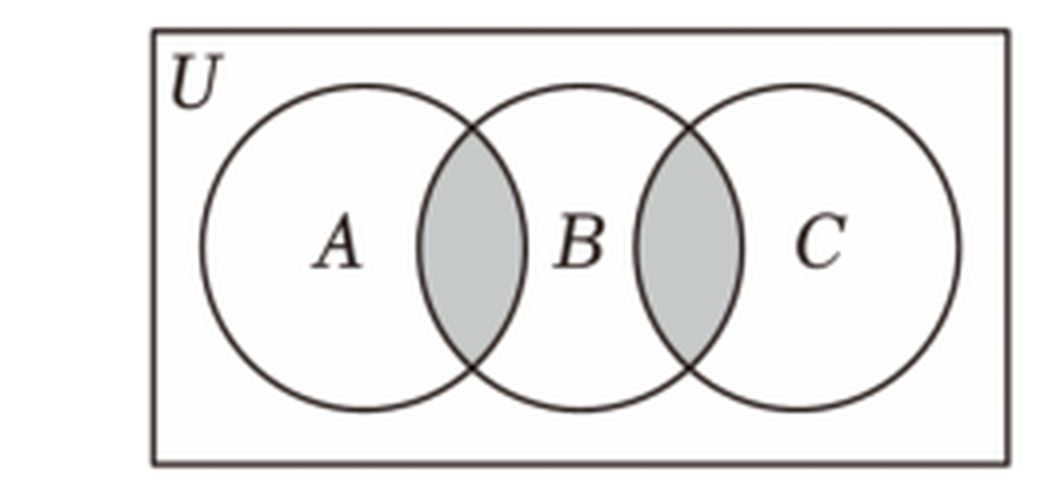
\includegraphics[width=0.30\textwidth]{figures/venn_ABC_lenses.png}
\end{center}

\keepwithprev
A. $B\cap(A\cup C)$\qquad\qquad\qquad B. $B\cap(A\cap C)$

C. $B\cap\complement_U(A\cup C)$\qquad\qquad D. $(A\cup B)\cap(B\cup C)$

\ans{$A$}

\ifanswer
\solbegin
\step{由图中阴影部分得，阴影为集合 $A$、$B$ 的交集和 $B$、$C$ 的交集的并集，}
\step{故阴影部分可表示为 $(A\cap B)\cup(B\cap C)$ 或 $B\cap(A\cup C)$，
故 $A$ 正确. 故选 $A$.}
\solend

\fi

\item 设集合 $P_1=\{x\mid x^2+ax+1>0\}$，$P_2=\{x\mid x^2+ax+2>0\}$，
$Q_1=\{x\mid x^2+x+b>0\}$，$Q_2=\{x\mid x^2+2x+b>0\}$，其中 $a$、$b\in\R$，
对于下列两个命题：①存在 $a$，$P_1$ 不是 $P_2$ 的子集；②存在 $b$ 使得 $Q_1$ 是 $Q_2$
的子集. 下列说法正确的是\mbox{（\quad）}

\keepwithprev
A. ①是真命题，②是假命题\qquad B. ①是假命题，②是真命题

C. ①②都是真命题\qquad\qquad\quad D. ①②都是假命题

\ans{$B$}

\ifanswer
\solbegin
\step{对于集合 $P_1=\{x\mid x^2+ax+1>0\}$，$P_2=\{x\mid x^2+ax+2>0\}$，}
\step{得当 $m\in P_1$ 时，即 $m^2+am+1>0$，得 $m^2+am+2>0$，}
\step{即有 $m\in P_2$，得对任意 $a$，$P_1$ 是 $P_2$ 的子集，故①错误；}
\step{对于集合 $Q_1=\{x\mid x^2+x+b>0\}$，$Q_2=\{x\mid x^2+2x+b>0\}$，}
\step{当 $b=6$ 时，$Q_1=\{x\mid x^2+x+6>0\}=\R$，$Q_2=\{x\mid x^2+2x+6>0\}=\R$，}
\step{得 $Q_1$ 是 $Q_2$ 的子集，所以存在 $b$，使得 $Q_1$ 是 $Q_2$ 的子集，故②正确；}
\step{故选 $B$.}
\solend

\fi

\item 设 $a$、$b\in\R$，则“$a+b>2$ 且 $ab>1$”是“$a>1$ 且 $b>1$”的\mbox{（\quad）}

\keepwithprev
A. 充要条件\qquad\qquad\qquad B. 充分不必要条件

C. 必要不充分条件\qquad\quad D. 既不充分又不必要条件

\ans{$C$}

\ifanswer
\solbegin
\step{因为 $a>1$ 且 $b>1$，所以 $a+b>2$ 且 $ab>1$，}
\step{若已知 $a+b>2$ 且 $ab>1$，可取 $a=\dfrac12$，$b=8$，也满足已知，}
\step{所以“$a+b>2$ 且 $ab>1$”是“$a>1$ 且 $b>1$”的必要不充分条件，故选 $C$.}
\solend

\fi

\item 十七世纪，数学家费马提出猜想：“对任意正整数 $n>2$，关于 $x$、$y$、$z$ 的方程
$x^n+y^n=z^n$ 没有正整数解”. 1995 年数学家安德鲁·怀尔斯发表了完成的证明过程，使它
终成费马大定理. 对费马大定理，若用反证法证明，第一步是假设猜想不成立，即\mbox{（\quad）}

\keepwithprev
A. 对任意正整数 $n>2$，关于 $x$、$y$、$z$ 的方程 $x^n+y^n=z^n$ 都有正整数解

B. 对任意正整数 $n>2$，关于 $x$、$y$、$z$ 的方程 $x^n+y^n=z^n$ 至少存在一组正整数解

C. 存在正整数 $n\leqslant2$，关于 $x$、$y$、$z$ 的方程 $x^n+y^n=z^n$ 至少存在一组正整数解

D. 存在正整数 $n>2$，关于 $x$、$y$、$z$ 的方程 $x^n+y^n=z^n$ 至少存在一组正整数解

\ans{$D$}

\end{enumerate}

\bigsec{三、解答题}

\begin{enumerate}
\setcounter{enumi}{16}

\item 已知 $a$、$b$、$c$ 都是实数，且 $a+b+c=0$，$abc=1$，求证：$a$、$b$、$c$ 中必有一个
大于 $\dfrac32$.

\ifanswer
\solbegin
\step{由 $a+b+c=0$，$abc=1$，得 $a$、$b$、$c$ 中一个正数，两个负数，}
\step{不妨设 $c>0$，由题意得 $a+b=-c,ab=\dfrac1c$，}
\step{由根与系数的关系得 $a$、$b$ 是关于 $x$ 的方程 $x^2+cx+\dfrac1c=0$ 的两个根，}
\step{则 $\Delta=c^2-\dfrac4c=\dfrac{c^3-4}{c}\geqslant0$，}
\step{因为 $c>0$，所以 $c^3\geqslant4$，得 $c\geqslant\sqrt[3]{4}$，}
\step{又 $\dfrac32=\sqrt[3]{\left(\dfrac32\right)^3}=\sqrt[3]{\dfrac{27}{8}}<\sqrt[3]{4}$，}
\step{所以 $c>\dfrac32$，即 $a$、$b$、$c$ 中必有一个大于 $\dfrac32$.}
\solend

\fi

\ansspace[6]

\item 已知关于 $x$ 的一元二次方程 $x^2-mx+4m^2-3=0$ 的两个实根分别为 $x_1,x_2$.

\begin{enumerate}[label=(\arabic*)]
\item $x_1,x_2$ 均为正根，求实数 $m$ 的取值范围；
\item 若 $x_1,x_2$ 满足：$x_1+x_2=x_1x_2$，求实数 $m$ 的值.
\end{enumerate}

\ifanswer
\solbegin
\stepm{(1)}{由 $x_1,x_2$ 均为正根，得}
\step{$\begin{cases}\Delta=(-m)^2-4(4m^2-3)\geqslant0\\ x_1+x_2=m>0\\ x_1\cdot x_2=4m^2-3>0\end{cases}$，}
\step{解得 $\begin{cases}-\dfrac{2\sqrt5}{5}\leqslant m\leqslant\dfrac{2\sqrt5}{5}\\[4pt]
m>0\\[4pt] m\leqslant-\dfrac{\sqrt3}{2}$ 或 $m\geqslant\dfrac{\sqrt3}{2}\end{cases}$，}
\step{即 $\dfrac{\sqrt3}{2}\leqslant m\leqslant\dfrac{2\sqrt5}{5}$；}
\stepm{(2)}{由 (1) 得
$\begin{cases}-\dfrac{2\sqrt5}{5}\leqslant m\leqslant\dfrac{2\sqrt5}{5}\\[4pt]
m=4m^2-3\end{cases}$，解得 $m=1$（舍去）或 $m=-\dfrac34$，}
\step{则 $m=-\dfrac34$.}
\solend

\fi

\ansspace[6]

\item 已知集合 $A=\{x\mid m-1<x<m^2+1\}$，$B=\{x\mid-2<x<2\}$.

\begin{enumerate}[label=(\arabic*)]
\item 当 $m=2$ 时，求 $A\cup B$、$A\cap B$、$\complement_R B$、$A\cap(\complement_R B)$；
\item 若“$x\in A$”是“$x\in B$”成立的必要不充分条件，求实数 $m$ 的取值范围.
\end{enumerate}

\ifanswer
\solbegin
\stepm{(1)}{$m=2$ 时，$A=\{x\mid1<x<5\}$，且 $B=\{x\mid-2<x<2\}$，}
\step{所以 $A\cup B=\{x\mid-2<x<5\}$，$A\cap B=\{x\mid1<x<2\}$，}
\step{$\complement_R B=\{x\mid x\leqslant-2$ 或 $x\geqslant2\}$，
$A\cap(\complement_R B)=\{x\mid2\leqslant x<5\}$；}
\stepm{(2)}{若“$x\in A$”是“$x\in B$”成立的必要不充分条件，则 $B\subset A$，}
\step{所以 $\begin{cases}m-1<-2\\ m^2+1\geqslant2\end{cases}$
或 $\begin{cases}m-1\leqslant-2\\ m^2+1>2\end{cases}$，解得 $m<-1$，}
\step{故 $m$ 的取值范围为 $(-\infty,-1)$.}
\solend

\fi

\ansspace[6]

\item 已知 $m\in\R$，集合 $A=\{x\mid|x-1|\leqslant2\}$，集合
$B=\{x\mid m-3<x\leqslant m+2\}$.

\begin{enumerate}[label=(\arabic*)]
\item 若“$x\in A$”是“$x\in B$”的充分不必要条件，求 $m$ 的取值范围；
\item 若命题“$\forall x\in B$，$x\in\complement_R A$”是真命题，求 $m$ 的取值范围；
\item 若命题“$\exists x\in A$，$x\in B$”是真命题，求 $m$ 的取值范围.
\end{enumerate}

\ifanswer
\solbegin
\stepm{(1)}{集合 $A=\{x\mid|x-1|\leqslant2\}=\{x\mid-1\leqslant x\leqslant3\}$，}
\step{若“$x\in A$”是“$x\in B$”的充分不必要条件，则 $A\subset B$，}
\step{所以 $\begin{cases}m-3<-1\\ 3\leqslant m+2\end{cases}$，解得 $1\leqslant m<2$，}
\step{当 $m=1$ 时，$B=\{x\mid-2<x\leqslant3\}$，符合题意，}
\step{所以 $m$ 的取值范围是 $\{m\mid1\leqslant m<2\}$.}
\stepm{(2)}{若命题“$\forall x\in B$，$x\in\complement_R A$”是真命题，则 $B\subset\complement_R A$，}
\step{又 $\complement_R A=\{x\mid x<-1$ 或 $x>3\}$，$B\neq\varnothing$，
所以 $m+2<-1$ 或 $m-3\geqslant3$，}
\step{解得 $m<-3$ 或 $m\geqslant6$，所以 $\{m\mid m<-3$ 或 $m\geqslant6\}$；}
\stepm{(3)}{因为 $\exists x\in A$，$x\in B$ 是真命题，所以 $A\cap B\neq\varnothing$，}
\step{当 $A\cap B=\varnothing$ 时，所以 $m+2<-1$ 或 $m-3\geqslant3$，
即 $m<-3$ 或 $m\geqslant6$，}
\step{所以当 $A\cap B\neq\varnothing$ 时，$m$ 的取值范围是 $\{m\mid-3\leqslant m<6\}$，}
\step{则 $m$ 的取值范围是 $\{m\mid-3\leqslant m<6\}$.}
\solend

\fi

\ansspace[6]

\item 对于函数 $f(x)$，若 $f(x_0)=x_0$，则称 $x_0$ 为 $f(x)$ 的“不动点”；若
$f[f(x_0)]=x_0$，则称 $x_0$ 为 $f(x)$ 的“稳定点”. 函数 $f(x)$ 的“不动点”和“稳定点”
的集合分别记为 $A$ 和 $B$，即 $A=\{x\mid f(x)=x\}$，$B=\{x\mid f[f(x)]=x\}$.

\begin{enumerate}[label=(\arabic*)]
\item 设函数 $f(x)=3x+4$，求集合 $A$ 和 $B$；
\item 求证：$A\sub B$；
\item 设函数 $f(x)=ax^2+bx+c(a\neq0)$，且 $A=\varnothing$，求证：$B=\varnothing$.
\end{enumerate}

\ifanswer
\solbegin
\stepm{(1)}{令 $f(x)=3x+4=x$，解得 $x=-2$，故有 $A=\{-2\}$，}
\step{由于 $f[f(x)]=3(3x+4)+4=9x+16$，}
\step{令 $9x+16=x$，得 $x=-2$，故有 $B=\{-2\}$；}
\stepm{(2)}{若 $A=\varnothing$，则 $A\sub B$ 显然成立；}
\step{若 $A\neq\varnothing$，设 $t\in A$，则 $f(t)=t$，$f(f(t))=f(t)=t$，}
\step{所以 $t\in B$，故 $A\sub B$.}
\stepm{(3)}{因为 $A=\{x\mid f(x)=x\}=\varnothing$，所以 $ax^2+bx+c=x$ 无解，}
\step{即 $\Delta=(b-1)^2-4a<0$，}
\step{①当 $a>0$ 时，二次函数 $y=f(x)-x$，}
\step{即 $y=ax^2+(b-1)x+c$ 的图象在 $x$ 轴的上方，}
\step{所以 $\forall x\in\R$，$f(x)-x>0$ 恒成立，所以 $\forall x\in\R$，
$f(x)>x$ 恒成立，}
\step{所以 $\forall x\in\R$，$f[f(x)]>f(x)>x$ 恒成立，即 $B=\varnothing$；}
\step{②当 $a<0$ 时，同理可证 $B=\varnothing$；}
\step{综上，对于函数 $f(x)=ax^2+bx+c(a\neq0)$，当 $A=\varnothing$ 时，$B=\varnothing$.}
\solend

\fi

\ansspace*[10]

\end{enumerate}

\end{document}
"
% 紧凑版：xelatex "\def\iscompact{1}% 高一26_交附闵行_周练2.tex
%   —— 高一上数学「2026-2027 年交附闵行高一上周练 2」（试卷版/答案版）
% 试卷版：xelatex 高一26_交附闵行_周练2.tex
% 答案版：xelatex "\def\isanswer{1}\input{高一26_交附闵行_周练2.tex}"
% 紧凑版：xelatex "\def\iscompact{1}\input{高一26_交附闵行_周练2.tex}"
%
% 原始材料是微信公众号图文（公众号「魔都数学加油站」连载「27学年高一 26」，2026-09-21 发布，
% 原文标题「27学年高一26——2026-2027年上海市交附闵行高一上周练2」），
% 正文为 10 张 PNG 页（1080×1527，各页同尺寸）。原文本身就是一份**讲评版**——
% 题目下方直接印出【解析】（本卷无单独的【答案】行，填空题答案都写在解析里）。
% 试题文字与解析均照原卷录入，未改内容。卷面的粉色斜水印「魔都数学加油站」属水印，未录入。
%
% 卷首标题：原卷印作「2026-2027 年交附闵行高一上周练 2」（公众号标题里的「上海市」
% 三字卷面标题行没有，本稿照卷面），年份区间按全稿惯例排 en dash，前缀照原卷保留「年」。
%
% 与原卷的排版差异（均已在 README「说明」中交代）：
%   ① 原文自**第 3 题**起（第 1、2 题未在该文中发布），故本稿题号亦自 3 起；
%   ② 原卷本就印有「一、填空题」「二、选择题」「三、解答题」三节标题，本稿照原卷分节，
%      只把标题改排成全稿统一的「大节标题」样式；
%   ③ 原卷第 16 题的答案「D」直接印在题干末尾的括号内（原卷把括号连同 D 单独占一行），
%      第 13—15 题的括号空着、答案写在解析末句「故选 A／B／C」里；填空题的答案也都嵌在
%      解析里，本稿统一改为试卷版隐去、答案版以 \ans{} 给出（选择题另附【解析】）；
%   ④ 子集符号原卷两种并用：第 4 题题干与第 8 题、第 21(2) 题等作带下划线的 $\subseteq$，
%      第 19(2)、20(1)(2) 题作真包含的 $\subset$，本稿分别照录为 $\sub$ 与 $\subset$；
%   ⑤ 补集符号原卷作 $\complement_R$、$\complement_U$（第 4 题命题④、第 13 题选项 C、
%      第 19—20 题），本稿照录；
%   ⑥ 原卷的实数集 R 一律作斜体（第 11 题「$a\in R$」、第 14 题「$a$、$b\in R$」与解析的
%      $\{x\mid x^2+x+6>0\}=R$ 等），本稿按全稿惯例统一写作 $\R$；
%   ⑦ 原卷填空的横线约两个字宽，本稿按全稿惯例统一排 \blankline[4.4em]；
%   ⑧ 原卷未印副标题，本稿按全稿惯例补出副标题「集合与常用逻辑用语」；
%   ⑨ 第 13 题的 Venn 图原卷印在题干右侧（第 5 页），本稿移至题干之后；
%      图取原卷截图、4× LANCZOS 放大（figures/venn_ABC_lenses.png，
%      阴影为 $A\cap B$ 与 $B\cap C$ 两个交带，即 $(A\cap B)\cup(B\cap C)$）。
%
% 原卷存疑一处（照抄原卷、未改，见源码中该处上方注释）：
%   ① 第 12 题【解析】首步的方程组里印 $t<2$，而其后三处与末行答案都作 $t\leqslant2$
%      （$\left[\dfrac85,\dfrac{17}{10}\right)\cup\left(\dfrac95,2\right]$ 含 $2$）——
%      按题意 $N=\left\{x\mid t-\dfrac35\leqslant x\leqslant t\right\}\sub\{x\mid1\leqslant x\leqslant2\}$
%      只要求 $t\leqslant2$（$t=2$ 时 $N=\left[\dfrac75,2\right]$ 确实含于其中），
%      故方程组里的 $t<2$ 应是原卷笔误；本稿两处都照原卷录入、未互相迁就。
% 另：第 20(3) 题解析末两行原卷即作同话重复，照原卷录入。

\documentclass[a4paper,11pt]{article}
\usepackage{common}

\begin{document}

\examtitlest[3]{2026--2027 年交附闵行高一上周练 2}{集合与常用逻辑用语}

\bigsec{一、填空题}

\begin{enumerate}
\setcounter{enumi}{2}

\item 命题甲：集合 $M=\{x\mid kx^2-2kx+1=0\}$ 为空集；命题乙：关于 $x$ 的不等式
$x^2+(k-1)x+4>0$ 的解集为 $\R$. 若命题甲、乙中有且只有一个是真命题，则实数 $k$ 的取
值范围是 \blankline[4.4em].

\ifanswer
\solbegin
\step{因为集合 $M=\{x\mid kx^2-2kx+1=0\}$ 为空集，}
\step{当 $k\neq0$ 时，$\Delta=(-2k)^2-4k<0$，解得 $0<k<1$，}
\step{当 $k=0$ 时，方程变为 $1=0$，无解，满足题意，故 $0\leqslant k<1$；}
\step{又关于 $x$ 的不等式 $x^2+(k-1)x+4>0$ 的解集为 $\R$，}
\step{所以 $\Delta'=(k-1)^2-4\times4<0$，解得 $-3<k<5$，}
\step{当甲命题为真，乙命题为假时，无解，}
\step{当甲命题为假，乙命题为真时，$k\in(-3,0)\cup[1,5)$.}
\solend

\fi

\item 对任意 $A$、$B\sub\R$，记 $A\oplus B=\{x\mid x\in A\cup B,x\notin A\cap B\}$，
并称 $A\oplus B$ 为集合 $A$、$B$ 的对称差. 例如：若 $A=\{1,2,3\},B=\{2,3,4\}$，
则 $A\oplus B=\{1,4\}$. 下列命题中，为真命题的是 \blankline[4.4em].

\keepwithprev
①若 $A$、$B\sub\R$ 且 $A\oplus B\sub A$，则 $A\sub B$

②若 $A$、$B\sub\R$ 且 $A\oplus B=\varnothing$，则 $A=B$

③若 $A$、$B\sub\R$ 且 $A\oplus B=B$，则 $A=\varnothing$

④对任意 $A$、$B\sub\R$，都有 $A\oplus B=\complement_R A\oplus\complement_R B$

\ans{②③④}

\ifanswer
\solbegin
\step{对于①，因为 $A\oplus B\sub A$，
所以 $\{x\mid x\in A\cup B,x\notin A\cap B\}\sub A$，}
\step{故 $B\sub A$，①错误；}
\step{对于②，$A$、$B\sub\R$ 且 $A\oplus B=\varnothing$，
则 $\varnothing=\{x\mid x\in A\cup B,x\notin A\cap B\}$，}
\step{即 $A\cup B=A\cap B$，所以 $A=B$，②正确；}
\step{对于③，$A$、$B\sub\R$ 且 $A\oplus B=B$，
则 $B=\{x\mid x\in A\cup B,x\notin A\cap B\}$，}
\step{故 $A\sub B$，且 $B$ 中元素不在 $A\cap B$ 中，故 $A=\varnothing$，③正确；}
\step{对于④，$\complement_R A\oplus\complement_R B
=\{x\mid x\in\complement_R A\cup\complement_R B,x\notin\complement_R A\cap\complement_R B\}$，}
\step{其中 $\complement_R A\cup\complement_R B=\complement_R(A\cap B)$，
$\complement_R A\cap\complement_R B=\complement_R(A\cup B)$，}
\step{故 $\complement_R A\oplus\complement_R B
=\{x\mid x\in\complement_R(A\cap B),x\notin\complement_R(A\cup B)\}
=\{x\mid x\in A\cup B,x\notin A\cap B\}$，}
\step{而 $A\oplus B=\{x\mid x\in A\cup B,x\notin A\cap B\}$，
故 $A\oplus B=\complement_R A\oplus\complement_R B$，④正确.}
\step{故正确的是②③④.}
\solend

\fi

\item 已知 $A=\{a_1,a_2,a_3,a_4\},B=\{a^2\mid a\in A\}$，其中 $a_1<a_2<a_3<a_4$，
且 $a_1$、$a_2$、$a_3$、$a_4$ 均为整数，若 $A\cap B=\{a_3,a_4\},a_1+a_3=0$，
且 $A\cup B$ 中的所有元素之和为 $270$，则集合 $A$ 中所有元素之和为 \blankline[4.4em].

\ifanswer
\solbegin
\step{$A=\{a_1,a_2,a_3,a_4\},B=\{a^2\mid a\in A\}$，
因为 $A\cap B=\{a_3,a_4\},a_1+a_3=0$，}
\step{所以 $A=\{a_1,a_2,a_3,a_4\},B=\left\{a_1^2,a_2^2,a_4^2\right\}$，}
\step{若 $a_1^2=a_3$，则 $a_1=-1,a_3=1$，则 $a_2=0$，
此时 $A=\{-1,0,1,a_4\},B=\{0,1,a_4^2\}$，}
\step{因为 $A\cup B$ 中的所有元素之和为 $270$，
所以 $-1+0+1+a_4+1+a_4^2=270$，}
\step{无正整数解，舍去；}
\step{若 $a_2^2=a_3$，① $a_4^2=a_4$，所以 $a_4=1$，矛盾；}
\step{② $a_1^2=a_4$，此时 $A\cup B=\left\{-a_2^2,a_2,a_2^2,a_1^2,a_4^2\right\}$，
所以 $a_2^8+a_2^4+a_2=270$，}
\step{所以 $a_2=-2$，此时 $a_1=-4,a_2=-2,a_3=4,a_4=16$；}
\step{若 $a_4^2=a_3$，显然不成立；}
\step{综上，集合 $A$ 中所有元素之和为 $-4-2+4+16=14$.}
\solend

\fi

\item 将集合 $M=\{a_1,a_2,a_3,\cdots,a_n\}$ 分拆成两个集合 $A_i$ 和 $B_j$，且
$M\supseteq A_i\cup B_j$，$A_i\cap B_j=\varnothing$，这样的分拆方法共有 \blankline[4.4em] 种.

\ifanswer
\solbegin
\step{按集合 $A_i$ 中的元素个数进行分类：}
\step{若 $A_i$ 中有 $0$ 个元素（即 $C_n^0$ 种）时，则 $B_j$ 有 $2^n$ 种，
共有 $2^nC_n^0$ 种；}
\step{若 $A_i$ 中有 $1$ 个元素（即 $C_n^1$ 种）时，则 $B_j$ 有 $2^{n-1}$ 种，
共有 $2^{n-1}C_n^1$ 种；}
\step{若 $A_i$ 中有 $2$ 个元素（即 $C_n^2$ 种）时，则 $B_j$ 有 $2^{n-2}$ 种，
共有 $2^{n-2}C_n^2$ 种；}
\step{若 $A_i$ 中有 $3$ 个元素（即 $C_n^3$ 种）时，则 $B_j$ 有 $2^{n-3}$ 种，
共有 $2^{n-3}C_n^3$ 种；}
\step{若 $A_i$ 中有 $n$ 个元素（即 $C_n^n$ 种）时，则 $B_j$ 有 $2^0$ 种，
共有 $2^0C_n^n$ 种；}
\step{得 $2^nC_n^0+2^{n-1}C_n^1+2^{n-2}C_n^2+\cdots+2^0C_n^n=(1+2)^n$，
故这样的分拆方法有 $3^n$ 种.}
\solend

\fi

\item 已知集合 $A=\{x\mid x<2,x\in\Z\}$，$B=\{x\mid x>0,x\in\Z\}$，则
$A\cap B=$ \blankline[4.4em].

\ifanswer
\solbegin
\step{因为 $A=\{x\mid x<2,x\in\Z\}$，$B=\{x\mid x>0,x\in\Z\}$，}
\step{所以 $A\cap B=\{x\mid0<x<2,x\in\Z\}=\{1\}$.}
\solend

\fi

\item 已知集合 $A=\{x\mid(a-1)x^2+3x-2=0\}$，$B=\{x\mid x^2-3x+2=0\}$，若
$A\sub B$，求实数 $a$ 的取值范围是 \blankline[4.4em].

\ifanswer
\solbegin
\step{由方程 $x^2-3x+2=0$，解得 $x=1$ 或 $x=2$，即 $B=\{1,2\}$，}
\step{因为 $A\sub B$，所以 $A=\varnothing$ 或 $A=\{1\}$ 或 $A=\{2\}$ 或 $A=\{1,2\}$，}
\step{当 $A=\varnothing$ 时，
则 $\begin{cases}a\neq1\\ \Delta=3^2-4(a-1)\times(-2)<0\end{cases}$，
解得 $a<-\dfrac18$；}
\step{将 $x=1$ 代入方程 $(a-1)x^2+3x-2=0$，得 $a=0$，}
\step{此时 $A=\{x\mid-x^2+3x-2=0\}=\{1,2\}$，满足条件；}
\step{将 $x=2$ 代入方程 $(a-1)x^2+3x-2=0$，得到 $a=0$，上面已经验证满足条件；}
\step{综上所述，$a$ 的取值范围是 $\left(-\infty,-\dfrac18\right)\cup\{0\}$.}
\solend

\fi

\item 已知方程 $x^2-3x+a=0$ 的两根都大于 $1$，则 $a$ 的取值范围为 \blankline[4.4em].

\ifanswer
\solbegin
\step{由题意得 $\Delta=9-4a\geqslant0$，$x_1+x_2=3$，$x_1x_2=a$，
所以 $a\leqslant\dfrac94$，}
\step{则 $(x_1-1)(x_2-1)=x_1x_2-(x_1+x_2)+1=a-3+1>0$，所以 $a>2$，}
\step{故 $a$ 的范围为 $\left(2,\dfrac94\right]$.}
\solend

\fi

\item 设 $x_1$、$x_2$ 是方程 $x^2+x-3=0$ 的两个实数根，则 $x_1^2-x_2+2024=$
\blankline[4.4em].

\ifanswer
\solbegin
\step{由题意得 $x_1^2=3-x_1$，$x_1+x_2=-1$，}
\step{则 $x_1^2-x_2+2024=3-x_1-x_2+2024=2027-(-1)=2028$.}
\solend

\fi

\item 已知 $a\in\R$，若关于 $x$ 的方程 $x^2+ax+a^2-8=0$ 有两个实根 $x_1$、$x_2$，且
$\dfrac1{x_1}+\dfrac1{x_2}=-\dfrac12$，则 $a$ 的值为 \blankline[4.4em].

\ifanswer
\solbegin
\step{由题意得 $\Delta=a^2-4(a^2-8)=32-3a^2\geqslant0$，
解得 $a^2\leqslant\dfrac{32}{3}$，}
\step{由韦达定理得 $x_1+x_2=-a$，$x_1x_2=a^2-8$，}
\step{则 $\dfrac1{x_1}+\dfrac1{x_2}=\dfrac{x_1+x_2}{x_1x_2}
=\dfrac{-a}{a^2-8}=-\dfrac12$，}
\step{即 $a^2-2a-8=(a-4)(a+2)=0$，解得 $a=4$ 或 $a=-2$.}
\step{又 $a^2\leqslant\dfrac{32}{3}$，则 $a=-2$.}
\solend

\fi

\item 定义集合 $P=\{x\mid a\leqslant x\leqslant b\}$ 的“长度”是 $b-a$，其中 $a$、
$b\in\R$. 已知集合 $M=\left\{x\mid\dfrac65\leqslant x\leqslant\dfrac{17}{10}\right\}$，
$N=\left\{x\mid t-\dfrac35\leqslant x\leqslant t\right\}$，且 $M$、$N$ 都是集合
$\{x\mid1\leqslant x\leqslant2\}$ 的子集，若集合 $M\cup N$ 的“长度”大于 $\dfrac35$，
则 $t$ 的取值范围是 \blankline[4.4em].

\ifanswer
\solbegin
\step{因为 $N=\left\{x\mid t-\dfrac35\leqslant x\leqslant t\right\}$
是集合 $\{x\mid1\leqslant x\leqslant2\}$ 的子集，}
% 注：下一行方程组里的 $t<2$ 系原卷所印（本稿照录），与其后三处及末行答案的
%     $t\leqslant2$ 自相矛盾——按题意应为 $t\leqslant2$，见文件头「原卷存疑」①。
\step{所以 $\begin{cases}t-\dfrac35\geqslant1\\[2pt] t<2\end{cases}$，
解得 $\dfrac85\leqslant t\leqslant2$，}
\step{又 $M=\left\{x\mid\dfrac65\leqslant x\leqslant\dfrac{17}{10}\right\}$，
得集合 $M$ 的“长度”为 $\dfrac{17}{10}-\dfrac65=\dfrac12$，}
\step{又 $N=\left\{x\mid t-\dfrac35\leqslant x\leqslant t\right\}$，
要使集合 $M\cup N$ 的“长度”大于 $\dfrac35$，}
\step{若 $M\cup N=\left\{x\mid t-\dfrac35\leqslant x\leqslant\dfrac{17}{10}\right\}$，
则 $\dfrac{17}{10}-t+\dfrac35>\dfrac35$，所以 $t<\dfrac{17}{10}$，}
\step{又 $\dfrac85\leqslant t\leqslant2$，所以 $\dfrac85\leqslant t<\dfrac{17}{10}$；}
\step{若 $M\cup N=\left\{x\mid\dfrac65\leqslant x\leqslant t\right\}$，
则 $t-\dfrac65>\dfrac35$，所以 $t>\dfrac95$，}
\step{又 $\dfrac85\leqslant t\leqslant2$，所以 $\dfrac95<t\leqslant2$；}
\step{则 $t$ 的取值范围是 $\left[\dfrac85,\dfrac{17}{10}\right)\cup\left(\dfrac95,2\right]$.}
\solend

\fi

\end{enumerate}

% 第 13 题是「题干 + 图 + 选项」约 5.7cm 的一整块（图 0.30\textwidth、宽高比 0.477 → 高 2.29cm，
% 加题干 1 行、选项 2 行与段间距）。`\keepwithprev` 只挡得住「题干—选项」之间，挡不住
% 夹在中间的图——实测断点落在题干之后，题干孤零零留在 p1、图与四个选项整页翻到 p2
% （切页审计的 A 类）。故照 高一30 第 4 题的成例先量一次页高；**守卫要放在 `\bigsec` 之前**
% 连节标题一起量（放标题之后会把「二、选择题」孤立在页末，正是 高一40 修过的那类 B 类）。
% 7cm ＝ 节标题约 1.1cm ＋ 第 13 题那块约 5.7cm（留少量余量）。
\needvspace{7cm}
\bigsec{二、选择题}

\begin{enumerate}
\setcounter{enumi}{12}

\item 图中阴影部分用集合符号可以表示为\mbox{（\quad）}

\begin{center}
% 图取原卷截图、4× LANCZOS 放大（原卷把图印在题干右侧，本稿移至此处，见文件头⑨）。
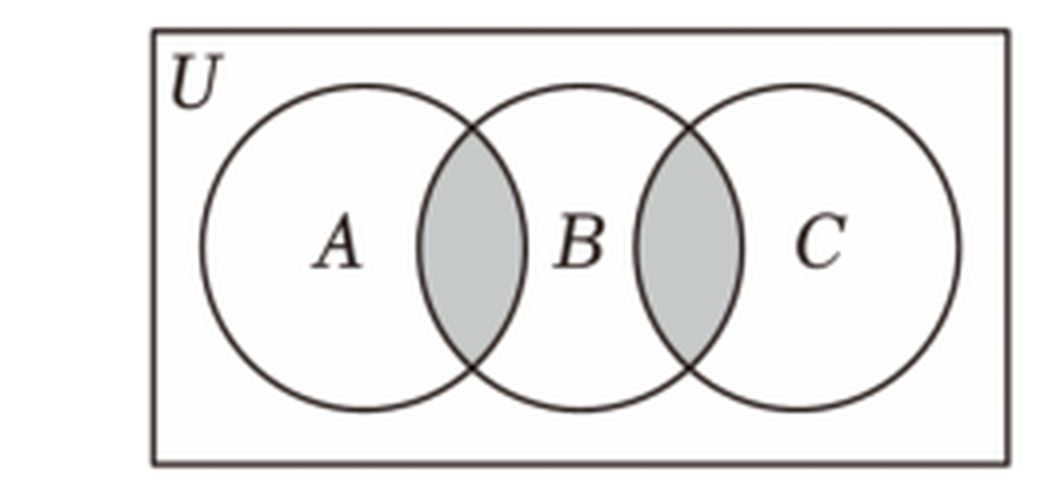
\includegraphics[width=0.30\textwidth]{figures/venn_ABC_lenses.png}
\end{center}

\keepwithprev
A. $B\cap(A\cup C)$\qquad\qquad\qquad B. $B\cap(A\cap C)$

C. $B\cap\complement_U(A\cup C)$\qquad\qquad D. $(A\cup B)\cap(B\cup C)$

\ans{$A$}

\ifanswer
\solbegin
\step{由图中阴影部分得，阴影为集合 $A$、$B$ 的交集和 $B$、$C$ 的交集的并集，}
\step{故阴影部分可表示为 $(A\cap B)\cup(B\cap C)$ 或 $B\cap(A\cup C)$，
故 $A$ 正确. 故选 $A$.}
\solend

\fi

\item 设集合 $P_1=\{x\mid x^2+ax+1>0\}$，$P_2=\{x\mid x^2+ax+2>0\}$，
$Q_1=\{x\mid x^2+x+b>0\}$，$Q_2=\{x\mid x^2+2x+b>0\}$，其中 $a$、$b\in\R$，
对于下列两个命题：①存在 $a$，$P_1$ 不是 $P_2$ 的子集；②存在 $b$ 使得 $Q_1$ 是 $Q_2$
的子集. 下列说法正确的是\mbox{（\quad）}

\keepwithprev
A. ①是真命题，②是假命题\qquad B. ①是假命题，②是真命题

C. ①②都是真命题\qquad\qquad\quad D. ①②都是假命题

\ans{$B$}

\ifanswer
\solbegin
\step{对于集合 $P_1=\{x\mid x^2+ax+1>0\}$，$P_2=\{x\mid x^2+ax+2>0\}$，}
\step{得当 $m\in P_1$ 时，即 $m^2+am+1>0$，得 $m^2+am+2>0$，}
\step{即有 $m\in P_2$，得对任意 $a$，$P_1$ 是 $P_2$ 的子集，故①错误；}
\step{对于集合 $Q_1=\{x\mid x^2+x+b>0\}$，$Q_2=\{x\mid x^2+2x+b>0\}$，}
\step{当 $b=6$ 时，$Q_1=\{x\mid x^2+x+6>0\}=\R$，$Q_2=\{x\mid x^2+2x+6>0\}=\R$，}
\step{得 $Q_1$ 是 $Q_2$ 的子集，所以存在 $b$，使得 $Q_1$ 是 $Q_2$ 的子集，故②正确；}
\step{故选 $B$.}
\solend

\fi

\item 设 $a$、$b\in\R$，则“$a+b>2$ 且 $ab>1$”是“$a>1$ 且 $b>1$”的\mbox{（\quad）}

\keepwithprev
A. 充要条件\qquad\qquad\qquad B. 充分不必要条件

C. 必要不充分条件\qquad\quad D. 既不充分又不必要条件

\ans{$C$}

\ifanswer
\solbegin
\step{因为 $a>1$ 且 $b>1$，所以 $a+b>2$ 且 $ab>1$，}
\step{若已知 $a+b>2$ 且 $ab>1$，可取 $a=\dfrac12$，$b=8$，也满足已知，}
\step{所以“$a+b>2$ 且 $ab>1$”是“$a>1$ 且 $b>1$”的必要不充分条件，故选 $C$.}
\solend

\fi

\item 十七世纪，数学家费马提出猜想：“对任意正整数 $n>2$，关于 $x$、$y$、$z$ 的方程
$x^n+y^n=z^n$ 没有正整数解”. 1995 年数学家安德鲁·怀尔斯发表了完成的证明过程，使它
终成费马大定理. 对费马大定理，若用反证法证明，第一步是假设猜想不成立，即\mbox{（\quad）}

\keepwithprev
A. 对任意正整数 $n>2$，关于 $x$、$y$、$z$ 的方程 $x^n+y^n=z^n$ 都有正整数解

B. 对任意正整数 $n>2$，关于 $x$、$y$、$z$ 的方程 $x^n+y^n=z^n$ 至少存在一组正整数解

C. 存在正整数 $n\leqslant2$，关于 $x$、$y$、$z$ 的方程 $x^n+y^n=z^n$ 至少存在一组正整数解

D. 存在正整数 $n>2$，关于 $x$、$y$、$z$ 的方程 $x^n+y^n=z^n$ 至少存在一组正整数解

\ans{$D$}

\end{enumerate}

\bigsec{三、解答题}

\begin{enumerate}
\setcounter{enumi}{16}

\item 已知 $a$、$b$、$c$ 都是实数，且 $a+b+c=0$，$abc=1$，求证：$a$、$b$、$c$ 中必有一个
大于 $\dfrac32$.

\ifanswer
\solbegin
\step{由 $a+b+c=0$，$abc=1$，得 $a$、$b$、$c$ 中一个正数，两个负数，}
\step{不妨设 $c>0$，由题意得 $a+b=-c,ab=\dfrac1c$，}
\step{由根与系数的关系得 $a$、$b$ 是关于 $x$ 的方程 $x^2+cx+\dfrac1c=0$ 的两个根，}
\step{则 $\Delta=c^2-\dfrac4c=\dfrac{c^3-4}{c}\geqslant0$，}
\step{因为 $c>0$，所以 $c^3\geqslant4$，得 $c\geqslant\sqrt[3]{4}$，}
\step{又 $\dfrac32=\sqrt[3]{\left(\dfrac32\right)^3}=\sqrt[3]{\dfrac{27}{8}}<\sqrt[3]{4}$，}
\step{所以 $c>\dfrac32$，即 $a$、$b$、$c$ 中必有一个大于 $\dfrac32$.}
\solend

\fi

\ansspace[6]

\item 已知关于 $x$ 的一元二次方程 $x^2-mx+4m^2-3=0$ 的两个实根分别为 $x_1,x_2$.

\begin{enumerate}[label=(\arabic*)]
\item $x_1,x_2$ 均为正根，求实数 $m$ 的取值范围；
\item 若 $x_1,x_2$ 满足：$x_1+x_2=x_1x_2$，求实数 $m$ 的值.
\end{enumerate}

\ifanswer
\solbegin
\stepm{(1)}{由 $x_1,x_2$ 均为正根，得}
\step{$\begin{cases}\Delta=(-m)^2-4(4m^2-3)\geqslant0\\ x_1+x_2=m>0\\ x_1\cdot x_2=4m^2-3>0\end{cases}$，}
\step{解得 $\begin{cases}-\dfrac{2\sqrt5}{5}\leqslant m\leqslant\dfrac{2\sqrt5}{5}\\[4pt]
m>0\\[4pt] m\leqslant-\dfrac{\sqrt3}{2}$ 或 $m\geqslant\dfrac{\sqrt3}{2}\end{cases}$，}
\step{即 $\dfrac{\sqrt3}{2}\leqslant m\leqslant\dfrac{2\sqrt5}{5}$；}
\stepm{(2)}{由 (1) 得
$\begin{cases}-\dfrac{2\sqrt5}{5}\leqslant m\leqslant\dfrac{2\sqrt5}{5}\\[4pt]
m=4m^2-3\end{cases}$，解得 $m=1$（舍去）或 $m=-\dfrac34$，}
\step{则 $m=-\dfrac34$.}
\solend

\fi

\ansspace[6]

\item 已知集合 $A=\{x\mid m-1<x<m^2+1\}$，$B=\{x\mid-2<x<2\}$.

\begin{enumerate}[label=(\arabic*)]
\item 当 $m=2$ 时，求 $A\cup B$、$A\cap B$、$\complement_R B$、$A\cap(\complement_R B)$；
\item 若“$x\in A$”是“$x\in B$”成立的必要不充分条件，求实数 $m$ 的取值范围.
\end{enumerate}

\ifanswer
\solbegin
\stepm{(1)}{$m=2$ 时，$A=\{x\mid1<x<5\}$，且 $B=\{x\mid-2<x<2\}$，}
\step{所以 $A\cup B=\{x\mid-2<x<5\}$，$A\cap B=\{x\mid1<x<2\}$，}
\step{$\complement_R B=\{x\mid x\leqslant-2$ 或 $x\geqslant2\}$，
$A\cap(\complement_R B)=\{x\mid2\leqslant x<5\}$；}
\stepm{(2)}{若“$x\in A$”是“$x\in B$”成立的必要不充分条件，则 $B\subset A$，}
\step{所以 $\begin{cases}m-1<-2\\ m^2+1\geqslant2\end{cases}$
或 $\begin{cases}m-1\leqslant-2\\ m^2+1>2\end{cases}$，解得 $m<-1$，}
\step{故 $m$ 的取值范围为 $(-\infty,-1)$.}
\solend

\fi

\ansspace[6]

\item 已知 $m\in\R$，集合 $A=\{x\mid|x-1|\leqslant2\}$，集合
$B=\{x\mid m-3<x\leqslant m+2\}$.

\begin{enumerate}[label=(\arabic*)]
\item 若“$x\in A$”是“$x\in B$”的充分不必要条件，求 $m$ 的取值范围；
\item 若命题“$\forall x\in B$，$x\in\complement_R A$”是真命题，求 $m$ 的取值范围；
\item 若命题“$\exists x\in A$，$x\in B$”是真命题，求 $m$ 的取值范围.
\end{enumerate}

\ifanswer
\solbegin
\stepm{(1)}{集合 $A=\{x\mid|x-1|\leqslant2\}=\{x\mid-1\leqslant x\leqslant3\}$，}
\step{若“$x\in A$”是“$x\in B$”的充分不必要条件，则 $A\subset B$，}
\step{所以 $\begin{cases}m-3<-1\\ 3\leqslant m+2\end{cases}$，解得 $1\leqslant m<2$，}
\step{当 $m=1$ 时，$B=\{x\mid-2<x\leqslant3\}$，符合题意，}
\step{所以 $m$ 的取值范围是 $\{m\mid1\leqslant m<2\}$.}
\stepm{(2)}{若命题“$\forall x\in B$，$x\in\complement_R A$”是真命题，则 $B\subset\complement_R A$，}
\step{又 $\complement_R A=\{x\mid x<-1$ 或 $x>3\}$，$B\neq\varnothing$，
所以 $m+2<-1$ 或 $m-3\geqslant3$，}
\step{解得 $m<-3$ 或 $m\geqslant6$，所以 $\{m\mid m<-3$ 或 $m\geqslant6\}$；}
\stepm{(3)}{因为 $\exists x\in A$，$x\in B$ 是真命题，所以 $A\cap B\neq\varnothing$，}
\step{当 $A\cap B=\varnothing$ 时，所以 $m+2<-1$ 或 $m-3\geqslant3$，
即 $m<-3$ 或 $m\geqslant6$，}
\step{所以当 $A\cap B\neq\varnothing$ 时，$m$ 的取值范围是 $\{m\mid-3\leqslant m<6\}$，}
\step{则 $m$ 的取值范围是 $\{m\mid-3\leqslant m<6\}$.}
\solend

\fi

\ansspace[6]

\item 对于函数 $f(x)$，若 $f(x_0)=x_0$，则称 $x_0$ 为 $f(x)$ 的“不动点”；若
$f[f(x_0)]=x_0$，则称 $x_0$ 为 $f(x)$ 的“稳定点”. 函数 $f(x)$ 的“不动点”和“稳定点”
的集合分别记为 $A$ 和 $B$，即 $A=\{x\mid f(x)=x\}$，$B=\{x\mid f[f(x)]=x\}$.

\begin{enumerate}[label=(\arabic*)]
\item 设函数 $f(x)=3x+4$，求集合 $A$ 和 $B$；
\item 求证：$A\sub B$；
\item 设函数 $f(x)=ax^2+bx+c(a\neq0)$，且 $A=\varnothing$，求证：$B=\varnothing$.
\end{enumerate}

\ifanswer
\solbegin
\stepm{(1)}{令 $f(x)=3x+4=x$，解得 $x=-2$，故有 $A=\{-2\}$，}
\step{由于 $f[f(x)]=3(3x+4)+4=9x+16$，}
\step{令 $9x+16=x$，得 $x=-2$，故有 $B=\{-2\}$；}
\stepm{(2)}{若 $A=\varnothing$，则 $A\sub B$ 显然成立；}
\step{若 $A\neq\varnothing$，设 $t\in A$，则 $f(t)=t$，$f(f(t))=f(t)=t$，}
\step{所以 $t\in B$，故 $A\sub B$.}
\stepm{(3)}{因为 $A=\{x\mid f(x)=x\}=\varnothing$，所以 $ax^2+bx+c=x$ 无解，}
\step{即 $\Delta=(b-1)^2-4a<0$，}
\step{①当 $a>0$ 时，二次函数 $y=f(x)-x$，}
\step{即 $y=ax^2+(b-1)x+c$ 的图象在 $x$ 轴的上方，}
\step{所以 $\forall x\in\R$，$f(x)-x>0$ 恒成立，所以 $\forall x\in\R$，
$f(x)>x$ 恒成立，}
\step{所以 $\forall x\in\R$，$f[f(x)]>f(x)>x$ 恒成立，即 $B=\varnothing$；}
\step{②当 $a<0$ 时，同理可证 $B=\varnothing$；}
\step{综上，对于函数 $f(x)=ax^2+bx+c(a\neq0)$，当 $A=\varnothing$ 时，$B=\varnothing$.}
\solend

\fi

\ansspace*[10]

\end{enumerate}

\end{document}
"
%
% 原始材料是微信公众号图文（公众号「魔都数学加油站」连载「27学年高一 26」，2026-09-21 发布，
% 原文标题「27学年高一26——2026-2027年上海市交附闵行高一上周练2」），
% 正文为 10 张 PNG 页（1080×1527，各页同尺寸）。原文本身就是一份**讲评版**——
% 题目下方直接印出【解析】（本卷无单独的【答案】行，填空题答案都写在解析里）。
% 试题文字与解析均照原卷录入，未改内容。卷面的粉色斜水印「魔都数学加油站」属水印，未录入。
%
% 卷首标题：原卷印作「2026-2027 年交附闵行高一上周练 2」（公众号标题里的「上海市」
% 三字卷面标题行没有，本稿照卷面），年份区间按全稿惯例排 en dash，前缀照原卷保留「年」。
%
% 与原卷的排版差异（均已在 README「说明」中交代）：
%   ① 原文自**第 3 题**起（第 1、2 题未在该文中发布），故本稿题号亦自 3 起；
%   ② 原卷本就印有「一、填空题」「二、选择题」「三、解答题」三节标题，本稿照原卷分节，
%      只把标题改排成全稿统一的「大节标题」样式；
%   ③ 原卷第 16 题的答案「D」直接印在题干末尾的括号内（原卷把括号连同 D 单独占一行），
%      第 13—15 题的括号空着、答案写在解析末句「故选 A／B／C」里；填空题的答案也都嵌在
%      解析里，本稿统一改为试卷版隐去、答案版以 \ans{} 给出（选择题另附【解析】）；
%   ④ 子集符号原卷两种并用：第 4 题题干与第 8 题、第 21(2) 题等作带下划线的 $\subseteq$，
%      第 19(2)、20(1)(2) 题作真包含的 $\subset$，本稿分别照录为 $\sub$ 与 $\subset$；
%   ⑤ 补集符号原卷作 $\complement_R$、$\complement_U$（第 4 题命题④、第 13 题选项 C、
%      第 19—20 题），本稿照录；
%   ⑥ 原卷的实数集 R 一律作斜体（第 11 题「$a\in R$」、第 14 题「$a$、$b\in R$」与解析的
%      $\{x\mid x^2+x+6>0\}=R$ 等），本稿按全稿惯例统一写作 $\R$；
%   ⑦ 原卷填空的横线约两个字宽，本稿按全稿惯例统一排 \blankline[4.4em]；
%   ⑧ 原卷未印副标题，本稿按全稿惯例补出副标题「集合与常用逻辑用语」；
%   ⑨ 第 13 题的 Venn 图原卷印在题干右侧（第 5 页），本稿移至题干之后；
%      图取原卷截图、4× LANCZOS 放大（figures/venn_ABC_lenses.png，
%      阴影为 $A\cap B$ 与 $B\cap C$ 两个交带，即 $(A\cap B)\cup(B\cap C)$）。
%
% 原卷存疑一处（照抄原卷、未改，见源码中该处上方注释）：
%   ① 第 12 题【解析】首步的方程组里印 $t<2$，而其后三处与末行答案都作 $t\leqslant2$
%      （$\left[\dfrac85,\dfrac{17}{10}\right)\cup\left(\dfrac95,2\right]$ 含 $2$）——
%      按题意 $N=\left\{x\mid t-\dfrac35\leqslant x\leqslant t\right\}\sub\{x\mid1\leqslant x\leqslant2\}$
%      只要求 $t\leqslant2$（$t=2$ 时 $N=\left[\dfrac75,2\right]$ 确实含于其中），
%      故方程组里的 $t<2$ 应是原卷笔误；本稿两处都照原卷录入、未互相迁就。
% 另：第 20(3) 题解析末两行原卷即作同话重复，照原卷录入。

\documentclass[a4paper,11pt]{article}
\usepackage{common}

\begin{document}

\examtitlest[3]{2026--2027 年交附闵行高一上周练 2}{集合与常用逻辑用语}

\bigsec{一、填空题}

\begin{enumerate}
\setcounter{enumi}{2}

\item 命题甲：集合 $M=\{x\mid kx^2-2kx+1=0\}$ 为空集；命题乙：关于 $x$ 的不等式
$x^2+(k-1)x+4>0$ 的解集为 $\R$. 若命题甲、乙中有且只有一个是真命题，则实数 $k$ 的取
值范围是 \blankline[4.4em].

\ifanswer
\solbegin
\step{因为集合 $M=\{x\mid kx^2-2kx+1=0\}$ 为空集，}
\step{当 $k\neq0$ 时，$\Delta=(-2k)^2-4k<0$，解得 $0<k<1$，}
\step{当 $k=0$ 时，方程变为 $1=0$，无解，满足题意，故 $0\leqslant k<1$；}
\step{又关于 $x$ 的不等式 $x^2+(k-1)x+4>0$ 的解集为 $\R$，}
\step{所以 $\Delta'=(k-1)^2-4\times4<0$，解得 $-3<k<5$，}
\step{当甲命题为真，乙命题为假时，无解，}
\step{当甲命题为假，乙命题为真时，$k\in(-3,0)\cup[1,5)$.}
\solend

\fi

\item 对任意 $A$、$B\sub\R$，记 $A\oplus B=\{x\mid x\in A\cup B,x\notin A\cap B\}$，
并称 $A\oplus B$ 为集合 $A$、$B$ 的对称差. 例如：若 $A=\{1,2,3\},B=\{2,3,4\}$，
则 $A\oplus B=\{1,4\}$. 下列命题中，为真命题的是 \blankline[4.4em].

\keepwithprev
①若 $A$、$B\sub\R$ 且 $A\oplus B\sub A$，则 $A\sub B$

②若 $A$、$B\sub\R$ 且 $A\oplus B=\varnothing$，则 $A=B$

③若 $A$、$B\sub\R$ 且 $A\oplus B=B$，则 $A=\varnothing$

④对任意 $A$、$B\sub\R$，都有 $A\oplus B=\complement_R A\oplus\complement_R B$

\ans{②③④}

\ifanswer
\solbegin
\step{对于①，因为 $A\oplus B\sub A$，
所以 $\{x\mid x\in A\cup B,x\notin A\cap B\}\sub A$，}
\step{故 $B\sub A$，①错误；}
\step{对于②，$A$、$B\sub\R$ 且 $A\oplus B=\varnothing$，
则 $\varnothing=\{x\mid x\in A\cup B,x\notin A\cap B\}$，}
\step{即 $A\cup B=A\cap B$，所以 $A=B$，②正确；}
\step{对于③，$A$、$B\sub\R$ 且 $A\oplus B=B$，
则 $B=\{x\mid x\in A\cup B,x\notin A\cap B\}$，}
\step{故 $A\sub B$，且 $B$ 中元素不在 $A\cap B$ 中，故 $A=\varnothing$，③正确；}
\step{对于④，$\complement_R A\oplus\complement_R B
=\{x\mid x\in\complement_R A\cup\complement_R B,x\notin\complement_R A\cap\complement_R B\}$，}
\step{其中 $\complement_R A\cup\complement_R B=\complement_R(A\cap B)$，
$\complement_R A\cap\complement_R B=\complement_R(A\cup B)$，}
\step{故 $\complement_R A\oplus\complement_R B
=\{x\mid x\in\complement_R(A\cap B),x\notin\complement_R(A\cup B)\}
=\{x\mid x\in A\cup B,x\notin A\cap B\}$，}
\step{而 $A\oplus B=\{x\mid x\in A\cup B,x\notin A\cap B\}$，
故 $A\oplus B=\complement_R A\oplus\complement_R B$，④正确.}
\step{故正确的是②③④.}
\solend

\fi

\item 已知 $A=\{a_1,a_2,a_3,a_4\},B=\{a^2\mid a\in A\}$，其中 $a_1<a_2<a_3<a_4$，
且 $a_1$、$a_2$、$a_3$、$a_4$ 均为整数，若 $A\cap B=\{a_3,a_4\},a_1+a_3=0$，
且 $A\cup B$ 中的所有元素之和为 $270$，则集合 $A$ 中所有元素之和为 \blankline[4.4em].

\ifanswer
\solbegin
\step{$A=\{a_1,a_2,a_3,a_4\},B=\{a^2\mid a\in A\}$，
因为 $A\cap B=\{a_3,a_4\},a_1+a_3=0$，}
\step{所以 $A=\{a_1,a_2,a_3,a_4\},B=\left\{a_1^2,a_2^2,a_4^2\right\}$，}
\step{若 $a_1^2=a_3$，则 $a_1=-1,a_3=1$，则 $a_2=0$，
此时 $A=\{-1,0,1,a_4\},B=\{0,1,a_4^2\}$，}
\step{因为 $A\cup B$ 中的所有元素之和为 $270$，
所以 $-1+0+1+a_4+1+a_4^2=270$，}
\step{无正整数解，舍去；}
\step{若 $a_2^2=a_3$，① $a_4^2=a_4$，所以 $a_4=1$，矛盾；}
\step{② $a_1^2=a_4$，此时 $A\cup B=\left\{-a_2^2,a_2,a_2^2,a_1^2,a_4^2\right\}$，
所以 $a_2^8+a_2^4+a_2=270$，}
\step{所以 $a_2=-2$，此时 $a_1=-4,a_2=-2,a_3=4,a_4=16$；}
\step{若 $a_4^2=a_3$，显然不成立；}
\step{综上，集合 $A$ 中所有元素之和为 $-4-2+4+16=14$.}
\solend

\fi

\item 将集合 $M=\{a_1,a_2,a_3,\cdots,a_n\}$ 分拆成两个集合 $A_i$ 和 $B_j$，且
$M\supseteq A_i\cup B_j$，$A_i\cap B_j=\varnothing$，这样的分拆方法共有 \blankline[4.4em] 种.

\ifanswer
\solbegin
\step{按集合 $A_i$ 中的元素个数进行分类：}
\step{若 $A_i$ 中有 $0$ 个元素（即 $C_n^0$ 种）时，则 $B_j$ 有 $2^n$ 种，
共有 $2^nC_n^0$ 种；}
\step{若 $A_i$ 中有 $1$ 个元素（即 $C_n^1$ 种）时，则 $B_j$ 有 $2^{n-1}$ 种，
共有 $2^{n-1}C_n^1$ 种；}
\step{若 $A_i$ 中有 $2$ 个元素（即 $C_n^2$ 种）时，则 $B_j$ 有 $2^{n-2}$ 种，
共有 $2^{n-2}C_n^2$ 种；}
\step{若 $A_i$ 中有 $3$ 个元素（即 $C_n^3$ 种）时，则 $B_j$ 有 $2^{n-3}$ 种，
共有 $2^{n-3}C_n^3$ 种；}
\step{若 $A_i$ 中有 $n$ 个元素（即 $C_n^n$ 种）时，则 $B_j$ 有 $2^0$ 种，
共有 $2^0C_n^n$ 种；}
\step{得 $2^nC_n^0+2^{n-1}C_n^1+2^{n-2}C_n^2+\cdots+2^0C_n^n=(1+2)^n$，
故这样的分拆方法有 $3^n$ 种.}
\solend

\fi

\item 已知集合 $A=\{x\mid x<2,x\in\Z\}$，$B=\{x\mid x>0,x\in\Z\}$，则
$A\cap B=$ \blankline[4.4em].

\ifanswer
\solbegin
\step{因为 $A=\{x\mid x<2,x\in\Z\}$，$B=\{x\mid x>0,x\in\Z\}$，}
\step{所以 $A\cap B=\{x\mid0<x<2,x\in\Z\}=\{1\}$.}
\solend

\fi

\item 已知集合 $A=\{x\mid(a-1)x^2+3x-2=0\}$，$B=\{x\mid x^2-3x+2=0\}$，若
$A\sub B$，求实数 $a$ 的取值范围是 \blankline[4.4em].

\ifanswer
\solbegin
\step{由方程 $x^2-3x+2=0$，解得 $x=1$ 或 $x=2$，即 $B=\{1,2\}$，}
\step{因为 $A\sub B$，所以 $A=\varnothing$ 或 $A=\{1\}$ 或 $A=\{2\}$ 或 $A=\{1,2\}$，}
\step{当 $A=\varnothing$ 时，
则 $\begin{cases}a\neq1\\ \Delta=3^2-4(a-1)\times(-2)<0\end{cases}$，
解得 $a<-\dfrac18$；}
\step{将 $x=1$ 代入方程 $(a-1)x^2+3x-2=0$，得 $a=0$，}
\step{此时 $A=\{x\mid-x^2+3x-2=0\}=\{1,2\}$，满足条件；}
\step{将 $x=2$ 代入方程 $(a-1)x^2+3x-2=0$，得到 $a=0$，上面已经验证满足条件；}
\step{综上所述，$a$ 的取值范围是 $\left(-\infty,-\dfrac18\right)\cup\{0\}$.}
\solend

\fi

\item 已知方程 $x^2-3x+a=0$ 的两根都大于 $1$，则 $a$ 的取值范围为 \blankline[4.4em].

\ifanswer
\solbegin
\step{由题意得 $\Delta=9-4a\geqslant0$，$x_1+x_2=3$，$x_1x_2=a$，
所以 $a\leqslant\dfrac94$，}
\step{则 $(x_1-1)(x_2-1)=x_1x_2-(x_1+x_2)+1=a-3+1>0$，所以 $a>2$，}
\step{故 $a$ 的范围为 $\left(2,\dfrac94\right]$.}
\solend

\fi

\item 设 $x_1$、$x_2$ 是方程 $x^2+x-3=0$ 的两个实数根，则 $x_1^2-x_2+2024=$
\blankline[4.4em].

\ifanswer
\solbegin
\step{由题意得 $x_1^2=3-x_1$，$x_1+x_2=-1$，}
\step{则 $x_1^2-x_2+2024=3-x_1-x_2+2024=2027-(-1)=2028$.}
\solend

\fi

\item 已知 $a\in\R$，若关于 $x$ 的方程 $x^2+ax+a^2-8=0$ 有两个实根 $x_1$、$x_2$，且
$\dfrac1{x_1}+\dfrac1{x_2}=-\dfrac12$，则 $a$ 的值为 \blankline[4.4em].

\ifanswer
\solbegin
\step{由题意得 $\Delta=a^2-4(a^2-8)=32-3a^2\geqslant0$，
解得 $a^2\leqslant\dfrac{32}{3}$，}
\step{由韦达定理得 $x_1+x_2=-a$，$x_1x_2=a^2-8$，}
\step{则 $\dfrac1{x_1}+\dfrac1{x_2}=\dfrac{x_1+x_2}{x_1x_2}
=\dfrac{-a}{a^2-8}=-\dfrac12$，}
\step{即 $a^2-2a-8=(a-4)(a+2)=0$，解得 $a=4$ 或 $a=-2$.}
\step{又 $a^2\leqslant\dfrac{32}{3}$，则 $a=-2$.}
\solend

\fi

\item 定义集合 $P=\{x\mid a\leqslant x\leqslant b\}$ 的“长度”是 $b-a$，其中 $a$、
$b\in\R$. 已知集合 $M=\left\{x\mid\dfrac65\leqslant x\leqslant\dfrac{17}{10}\right\}$，
$N=\left\{x\mid t-\dfrac35\leqslant x\leqslant t\right\}$，且 $M$、$N$ 都是集合
$\{x\mid1\leqslant x\leqslant2\}$ 的子集，若集合 $M\cup N$ 的“长度”大于 $\dfrac35$，
则 $t$ 的取值范围是 \blankline[4.4em].

\ifanswer
\solbegin
\step{因为 $N=\left\{x\mid t-\dfrac35\leqslant x\leqslant t\right\}$
是集合 $\{x\mid1\leqslant x\leqslant2\}$ 的子集，}
% 注：下一行方程组里的 $t<2$ 系原卷所印（本稿照录），与其后三处及末行答案的
%     $t\leqslant2$ 自相矛盾——按题意应为 $t\leqslant2$，见文件头「原卷存疑」①。
\step{所以 $\begin{cases}t-\dfrac35\geqslant1\\[2pt] t<2\end{cases}$，
解得 $\dfrac85\leqslant t\leqslant2$，}
\step{又 $M=\left\{x\mid\dfrac65\leqslant x\leqslant\dfrac{17}{10}\right\}$，
得集合 $M$ 的“长度”为 $\dfrac{17}{10}-\dfrac65=\dfrac12$，}
\step{又 $N=\left\{x\mid t-\dfrac35\leqslant x\leqslant t\right\}$，
要使集合 $M\cup N$ 的“长度”大于 $\dfrac35$，}
\step{若 $M\cup N=\left\{x\mid t-\dfrac35\leqslant x\leqslant\dfrac{17}{10}\right\}$，
则 $\dfrac{17}{10}-t+\dfrac35>\dfrac35$，所以 $t<\dfrac{17}{10}$，}
\step{又 $\dfrac85\leqslant t\leqslant2$，所以 $\dfrac85\leqslant t<\dfrac{17}{10}$；}
\step{若 $M\cup N=\left\{x\mid\dfrac65\leqslant x\leqslant t\right\}$，
则 $t-\dfrac65>\dfrac35$，所以 $t>\dfrac95$，}
\step{又 $\dfrac85\leqslant t\leqslant2$，所以 $\dfrac95<t\leqslant2$；}
\step{则 $t$ 的取值范围是 $\left[\dfrac85,\dfrac{17}{10}\right)\cup\left(\dfrac95,2\right]$.}
\solend

\fi

\end{enumerate}

% 第 13 题是「题干 + 图 + 选项」约 5.7cm 的一整块（图 0.30\textwidth、宽高比 0.477 → 高 2.29cm，
% 加题干 1 行、选项 2 行与段间距）。`\keepwithprev` 只挡得住「题干—选项」之间，挡不住
% 夹在中间的图——实测断点落在题干之后，题干孤零零留在 p1、图与四个选项整页翻到 p2
% （切页审计的 A 类）。故照 高一30 第 4 题的成例先量一次页高；**守卫要放在 `\bigsec` 之前**
% 连节标题一起量（放标题之后会把「二、选择题」孤立在页末，正是 高一40 修过的那类 B 类）。
% 7cm ＝ 节标题约 1.1cm ＋ 第 13 题那块约 5.7cm（留少量余量）。
\needvspace{7cm}
\bigsec{二、选择题}

\begin{enumerate}
\setcounter{enumi}{12}

\item 图中阴影部分用集合符号可以表示为\mbox{（\quad）}

\begin{center}
% 图取原卷截图、4× LANCZOS 放大（原卷把图印在题干右侧，本稿移至此处，见文件头⑨）。
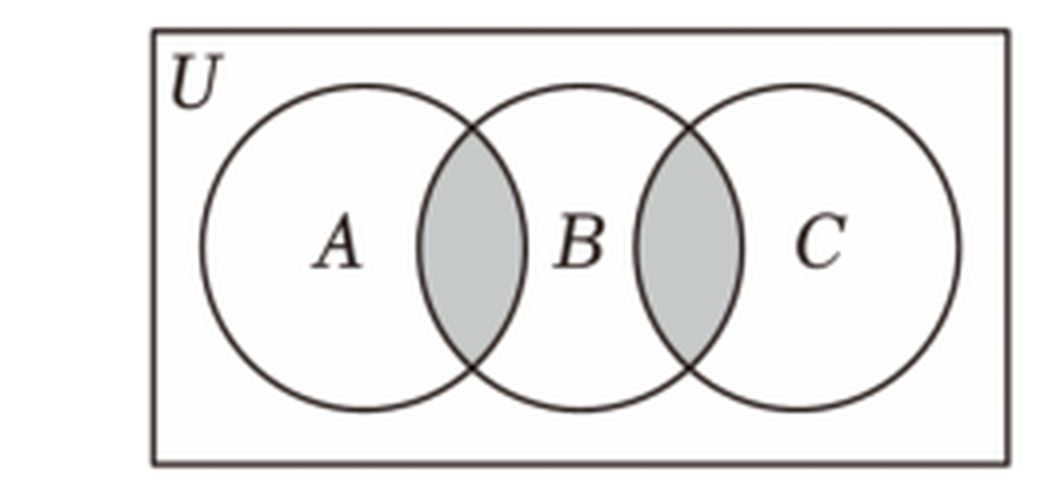
\includegraphics[width=0.30\textwidth]{figures/venn_ABC_lenses.png}
\end{center}

\keepwithprev
A. $B\cap(A\cup C)$\qquad\qquad\qquad B. $B\cap(A\cap C)$

C. $B\cap\complement_U(A\cup C)$\qquad\qquad D. $(A\cup B)\cap(B\cup C)$

\ans{$A$}

\ifanswer
\solbegin
\step{由图中阴影部分得，阴影为集合 $A$、$B$ 的交集和 $B$、$C$ 的交集的并集，}
\step{故阴影部分可表示为 $(A\cap B)\cup(B\cap C)$ 或 $B\cap(A\cup C)$，
故 $A$ 正确. 故选 $A$.}
\solend

\fi

\item 设集合 $P_1=\{x\mid x^2+ax+1>0\}$，$P_2=\{x\mid x^2+ax+2>0\}$，
$Q_1=\{x\mid x^2+x+b>0\}$，$Q_2=\{x\mid x^2+2x+b>0\}$，其中 $a$、$b\in\R$，
对于下列两个命题：①存在 $a$，$P_1$ 不是 $P_2$ 的子集；②存在 $b$ 使得 $Q_1$ 是 $Q_2$
的子集. 下列说法正确的是\mbox{（\quad）}

\keepwithprev
A. ①是真命题，②是假命题\qquad B. ①是假命题，②是真命题

C. ①②都是真命题\qquad\qquad\quad D. ①②都是假命题

\ans{$B$}

\ifanswer
\solbegin
\step{对于集合 $P_1=\{x\mid x^2+ax+1>0\}$，$P_2=\{x\mid x^2+ax+2>0\}$，}
\step{得当 $m\in P_1$ 时，即 $m^2+am+1>0$，得 $m^2+am+2>0$，}
\step{即有 $m\in P_2$，得对任意 $a$，$P_1$ 是 $P_2$ 的子集，故①错误；}
\step{对于集合 $Q_1=\{x\mid x^2+x+b>0\}$，$Q_2=\{x\mid x^2+2x+b>0\}$，}
\step{当 $b=6$ 时，$Q_1=\{x\mid x^2+x+6>0\}=\R$，$Q_2=\{x\mid x^2+2x+6>0\}=\R$，}
\step{得 $Q_1$ 是 $Q_2$ 的子集，所以存在 $b$，使得 $Q_1$ 是 $Q_2$ 的子集，故②正确；}
\step{故选 $B$.}
\solend

\fi

\item 设 $a$、$b\in\R$，则“$a+b>2$ 且 $ab>1$”是“$a>1$ 且 $b>1$”的\mbox{（\quad）}

\keepwithprev
A. 充要条件\qquad\qquad\qquad B. 充分不必要条件

C. 必要不充分条件\qquad\quad D. 既不充分又不必要条件

\ans{$C$}

\ifanswer
\solbegin
\step{因为 $a>1$ 且 $b>1$，所以 $a+b>2$ 且 $ab>1$，}
\step{若已知 $a+b>2$ 且 $ab>1$，可取 $a=\dfrac12$，$b=8$，也满足已知，}
\step{所以“$a+b>2$ 且 $ab>1$”是“$a>1$ 且 $b>1$”的必要不充分条件，故选 $C$.}
\solend

\fi

\item 十七世纪，数学家费马提出猜想：“对任意正整数 $n>2$，关于 $x$、$y$、$z$ 的方程
$x^n+y^n=z^n$ 没有正整数解”. 1995 年数学家安德鲁·怀尔斯发表了完成的证明过程，使它
终成费马大定理. 对费马大定理，若用反证法证明，第一步是假设猜想不成立，即\mbox{（\quad）}

\keepwithprev
A. 对任意正整数 $n>2$，关于 $x$、$y$、$z$ 的方程 $x^n+y^n=z^n$ 都有正整数解

B. 对任意正整数 $n>2$，关于 $x$、$y$、$z$ 的方程 $x^n+y^n=z^n$ 至少存在一组正整数解

C. 存在正整数 $n\leqslant2$，关于 $x$、$y$、$z$ 的方程 $x^n+y^n=z^n$ 至少存在一组正整数解

D. 存在正整数 $n>2$，关于 $x$、$y$、$z$ 的方程 $x^n+y^n=z^n$ 至少存在一组正整数解

\ans{$D$}

\end{enumerate}

\bigsec{三、解答题}

\begin{enumerate}
\setcounter{enumi}{16}

\item 已知 $a$、$b$、$c$ 都是实数，且 $a+b+c=0$，$abc=1$，求证：$a$、$b$、$c$ 中必有一个
大于 $\dfrac32$.

\ifanswer
\solbegin
\step{由 $a+b+c=0$，$abc=1$，得 $a$、$b$、$c$ 中一个正数，两个负数，}
\step{不妨设 $c>0$，由题意得 $a+b=-c,ab=\dfrac1c$，}
\step{由根与系数的关系得 $a$、$b$ 是关于 $x$ 的方程 $x^2+cx+\dfrac1c=0$ 的两个根，}
\step{则 $\Delta=c^2-\dfrac4c=\dfrac{c^3-4}{c}\geqslant0$，}
\step{因为 $c>0$，所以 $c^3\geqslant4$，得 $c\geqslant\sqrt[3]{4}$，}
\step{又 $\dfrac32=\sqrt[3]{\left(\dfrac32\right)^3}=\sqrt[3]{\dfrac{27}{8}}<\sqrt[3]{4}$，}
\step{所以 $c>\dfrac32$，即 $a$、$b$、$c$ 中必有一个大于 $\dfrac32$.}
\solend

\fi

\ansspace[6]

\item 已知关于 $x$ 的一元二次方程 $x^2-mx+4m^2-3=0$ 的两个实根分别为 $x_1,x_2$.

\begin{enumerate}[label=(\arabic*)]
\item $x_1,x_2$ 均为正根，求实数 $m$ 的取值范围；
\item 若 $x_1,x_2$ 满足：$x_1+x_2=x_1x_2$，求实数 $m$ 的值.
\end{enumerate}

\ifanswer
\solbegin
\stepm{(1)}{由 $x_1,x_2$ 均为正根，得}
\step{$\begin{cases}\Delta=(-m)^2-4(4m^2-3)\geqslant0\\ x_1+x_2=m>0\\ x_1\cdot x_2=4m^2-3>0\end{cases}$，}
\step{解得 $\begin{cases}-\dfrac{2\sqrt5}{5}\leqslant m\leqslant\dfrac{2\sqrt5}{5}\\[4pt]
m>0\\[4pt] m\leqslant-\dfrac{\sqrt3}{2}$ 或 $m\geqslant\dfrac{\sqrt3}{2}\end{cases}$，}
\step{即 $\dfrac{\sqrt3}{2}\leqslant m\leqslant\dfrac{2\sqrt5}{5}$；}
\stepm{(2)}{由 (1) 得
$\begin{cases}-\dfrac{2\sqrt5}{5}\leqslant m\leqslant\dfrac{2\sqrt5}{5}\\[4pt]
m=4m^2-3\end{cases}$，解得 $m=1$（舍去）或 $m=-\dfrac34$，}
\step{则 $m=-\dfrac34$.}
\solend

\fi

\ansspace[6]

\item 已知集合 $A=\{x\mid m-1<x<m^2+1\}$，$B=\{x\mid-2<x<2\}$.

\begin{enumerate}[label=(\arabic*)]
\item 当 $m=2$ 时，求 $A\cup B$、$A\cap B$、$\complement_R B$、$A\cap(\complement_R B)$；
\item 若“$x\in A$”是“$x\in B$”成立的必要不充分条件，求实数 $m$ 的取值范围.
\end{enumerate}

\ifanswer
\solbegin
\stepm{(1)}{$m=2$ 时，$A=\{x\mid1<x<5\}$，且 $B=\{x\mid-2<x<2\}$，}
\step{所以 $A\cup B=\{x\mid-2<x<5\}$，$A\cap B=\{x\mid1<x<2\}$，}
\step{$\complement_R B=\{x\mid x\leqslant-2$ 或 $x\geqslant2\}$，
$A\cap(\complement_R B)=\{x\mid2\leqslant x<5\}$；}
\stepm{(2)}{若“$x\in A$”是“$x\in B$”成立的必要不充分条件，则 $B\subset A$，}
\step{所以 $\begin{cases}m-1<-2\\ m^2+1\geqslant2\end{cases}$
或 $\begin{cases}m-1\leqslant-2\\ m^2+1>2\end{cases}$，解得 $m<-1$，}
\step{故 $m$ 的取值范围为 $(-\infty,-1)$.}
\solend

\fi

\ansspace[6]

\item 已知 $m\in\R$，集合 $A=\{x\mid|x-1|\leqslant2\}$，集合
$B=\{x\mid m-3<x\leqslant m+2\}$.

\begin{enumerate}[label=(\arabic*)]
\item 若“$x\in A$”是“$x\in B$”的充分不必要条件，求 $m$ 的取值范围；
\item 若命题“$\forall x\in B$，$x\in\complement_R A$”是真命题，求 $m$ 的取值范围；
\item 若命题“$\exists x\in A$，$x\in B$”是真命题，求 $m$ 的取值范围.
\end{enumerate}

\ifanswer
\solbegin
\stepm{(1)}{集合 $A=\{x\mid|x-1|\leqslant2\}=\{x\mid-1\leqslant x\leqslant3\}$，}
\step{若“$x\in A$”是“$x\in B$”的充分不必要条件，则 $A\subset B$，}
\step{所以 $\begin{cases}m-3<-1\\ 3\leqslant m+2\end{cases}$，解得 $1\leqslant m<2$，}
\step{当 $m=1$ 时，$B=\{x\mid-2<x\leqslant3\}$，符合题意，}
\step{所以 $m$ 的取值范围是 $\{m\mid1\leqslant m<2\}$.}
\stepm{(2)}{若命题“$\forall x\in B$，$x\in\complement_R A$”是真命题，则 $B\subset\complement_R A$，}
\step{又 $\complement_R A=\{x\mid x<-1$ 或 $x>3\}$，$B\neq\varnothing$，
所以 $m+2<-1$ 或 $m-3\geqslant3$，}
\step{解得 $m<-3$ 或 $m\geqslant6$，所以 $\{m\mid m<-3$ 或 $m\geqslant6\}$；}
\stepm{(3)}{因为 $\exists x\in A$，$x\in B$ 是真命题，所以 $A\cap B\neq\varnothing$，}
\step{当 $A\cap B=\varnothing$ 时，所以 $m+2<-1$ 或 $m-3\geqslant3$，
即 $m<-3$ 或 $m\geqslant6$，}
\step{所以当 $A\cap B\neq\varnothing$ 时，$m$ 的取值范围是 $\{m\mid-3\leqslant m<6\}$，}
\step{则 $m$ 的取值范围是 $\{m\mid-3\leqslant m<6\}$.}
\solend

\fi

\ansspace[6]

\item 对于函数 $f(x)$，若 $f(x_0)=x_0$，则称 $x_0$ 为 $f(x)$ 的“不动点”；若
$f[f(x_0)]=x_0$，则称 $x_0$ 为 $f(x)$ 的“稳定点”. 函数 $f(x)$ 的“不动点”和“稳定点”
的集合分别记为 $A$ 和 $B$，即 $A=\{x\mid f(x)=x\}$，$B=\{x\mid f[f(x)]=x\}$.

\begin{enumerate}[label=(\arabic*)]
\item 设函数 $f(x)=3x+4$，求集合 $A$ 和 $B$；
\item 求证：$A\sub B$；
\item 设函数 $f(x)=ax^2+bx+c(a\neq0)$，且 $A=\varnothing$，求证：$B=\varnothing$.
\end{enumerate}

\ifanswer
\solbegin
\stepm{(1)}{令 $f(x)=3x+4=x$，解得 $x=-2$，故有 $A=\{-2\}$，}
\step{由于 $f[f(x)]=3(3x+4)+4=9x+16$，}
\step{令 $9x+16=x$，得 $x=-2$，故有 $B=\{-2\}$；}
\stepm{(2)}{若 $A=\varnothing$，则 $A\sub B$ 显然成立；}
\step{若 $A\neq\varnothing$，设 $t\in A$，则 $f(t)=t$，$f(f(t))=f(t)=t$，}
\step{所以 $t\in B$，故 $A\sub B$.}
\stepm{(3)}{因为 $A=\{x\mid f(x)=x\}=\varnothing$，所以 $ax^2+bx+c=x$ 无解，}
\step{即 $\Delta=(b-1)^2-4a<0$，}
\step{①当 $a>0$ 时，二次函数 $y=f(x)-x$，}
\step{即 $y=ax^2+(b-1)x+c$ 的图象在 $x$ 轴的上方，}
\step{所以 $\forall x\in\R$，$f(x)-x>0$ 恒成立，所以 $\forall x\in\R$，
$f(x)>x$ 恒成立，}
\step{所以 $\forall x\in\R$，$f[f(x)]>f(x)>x$ 恒成立，即 $B=\varnothing$；}
\step{②当 $a<0$ 时，同理可证 $B=\varnothing$；}
\step{综上，对于函数 $f(x)=ax^2+bx+c(a\neq0)$，当 $A=\varnothing$ 时，$B=\varnothing$.}
\solend

\fi

\ansspace*[10]

\end{enumerate}

\end{document}
"
% 紧凑版：xelatex "\def\iscompact{1}% 高一26_交附闵行_周练2.tex
%   —— 高一上数学「2026-2027 年交附闵行高一上周练 2」（试卷版/答案版）
% 试卷版：xelatex 高一26_交附闵行_周练2.tex
% 答案版：xelatex "\def\isanswer{1}% 高一26_交附闵行_周练2.tex
%   —— 高一上数学「2026-2027 年交附闵行高一上周练 2」（试卷版/答案版）
% 试卷版：xelatex 高一26_交附闵行_周练2.tex
% 答案版：xelatex "\def\isanswer{1}\input{高一26_交附闵行_周练2.tex}"
% 紧凑版：xelatex "\def\iscompact{1}\input{高一26_交附闵行_周练2.tex}"
%
% 原始材料是微信公众号图文（公众号「魔都数学加油站」连载「27学年高一 26」，2026-09-21 发布，
% 原文标题「27学年高一26——2026-2027年上海市交附闵行高一上周练2」），
% 正文为 10 张 PNG 页（1080×1527，各页同尺寸）。原文本身就是一份**讲评版**——
% 题目下方直接印出【解析】（本卷无单独的【答案】行，填空题答案都写在解析里）。
% 试题文字与解析均照原卷录入，未改内容。卷面的粉色斜水印「魔都数学加油站」属水印，未录入。
%
% 卷首标题：原卷印作「2026-2027 年交附闵行高一上周练 2」（公众号标题里的「上海市」
% 三字卷面标题行没有，本稿照卷面），年份区间按全稿惯例排 en dash，前缀照原卷保留「年」。
%
% 与原卷的排版差异（均已在 README「说明」中交代）：
%   ① 原文自**第 3 题**起（第 1、2 题未在该文中发布），故本稿题号亦自 3 起；
%   ② 原卷本就印有「一、填空题」「二、选择题」「三、解答题」三节标题，本稿照原卷分节，
%      只把标题改排成全稿统一的「大节标题」样式；
%   ③ 原卷第 16 题的答案「D」直接印在题干末尾的括号内（原卷把括号连同 D 单独占一行），
%      第 13—15 题的括号空着、答案写在解析末句「故选 A／B／C」里；填空题的答案也都嵌在
%      解析里，本稿统一改为试卷版隐去、答案版以 \ans{} 给出（选择题另附【解析】）；
%   ④ 子集符号原卷两种并用：第 4 题题干与第 8 题、第 21(2) 题等作带下划线的 $\subseteq$，
%      第 19(2)、20(1)(2) 题作真包含的 $\subset$，本稿分别照录为 $\sub$ 与 $\subset$；
%   ⑤ 补集符号原卷作 $\complement_R$、$\complement_U$（第 4 题命题④、第 13 题选项 C、
%      第 19—20 题），本稿照录；
%   ⑥ 原卷的实数集 R 一律作斜体（第 11 题「$a\in R$」、第 14 题「$a$、$b\in R$」与解析的
%      $\{x\mid x^2+x+6>0\}=R$ 等），本稿按全稿惯例统一写作 $\R$；
%   ⑦ 原卷填空的横线约两个字宽，本稿按全稿惯例统一排 \blankline[4.4em]；
%   ⑧ 原卷未印副标题，本稿按全稿惯例补出副标题「集合与常用逻辑用语」；
%   ⑨ 第 13 题的 Venn 图原卷印在题干右侧（第 5 页），本稿移至题干之后；
%      图取原卷截图、4× LANCZOS 放大（figures/venn_ABC_lenses.png，
%      阴影为 $A\cap B$ 与 $B\cap C$ 两个交带，即 $(A\cap B)\cup(B\cap C)$）。
%
% 原卷存疑一处（照抄原卷、未改，见源码中该处上方注释）：
%   ① 第 12 题【解析】首步的方程组里印 $t<2$，而其后三处与末行答案都作 $t\leqslant2$
%      （$\left[\dfrac85,\dfrac{17}{10}\right)\cup\left(\dfrac95,2\right]$ 含 $2$）——
%      按题意 $N=\left\{x\mid t-\dfrac35\leqslant x\leqslant t\right\}\sub\{x\mid1\leqslant x\leqslant2\}$
%      只要求 $t\leqslant2$（$t=2$ 时 $N=\left[\dfrac75,2\right]$ 确实含于其中），
%      故方程组里的 $t<2$ 应是原卷笔误；本稿两处都照原卷录入、未互相迁就。
% 另：第 20(3) 题解析末两行原卷即作同话重复，照原卷录入。

\documentclass[a4paper,11pt]{article}
\usepackage{common}

\begin{document}

\examtitlest[3]{2026--2027 年交附闵行高一上周练 2}{集合与常用逻辑用语}

\bigsec{一、填空题}

\begin{enumerate}
\setcounter{enumi}{2}

\item 命题甲：集合 $M=\{x\mid kx^2-2kx+1=0\}$ 为空集；命题乙：关于 $x$ 的不等式
$x^2+(k-1)x+4>0$ 的解集为 $\R$. 若命题甲、乙中有且只有一个是真命题，则实数 $k$ 的取
值范围是 \blankline[4.4em].

\ifanswer
\solbegin
\step{因为集合 $M=\{x\mid kx^2-2kx+1=0\}$ 为空集，}
\step{当 $k\neq0$ 时，$\Delta=(-2k)^2-4k<0$，解得 $0<k<1$，}
\step{当 $k=0$ 时，方程变为 $1=0$，无解，满足题意，故 $0\leqslant k<1$；}
\step{又关于 $x$ 的不等式 $x^2+(k-1)x+4>0$ 的解集为 $\R$，}
\step{所以 $\Delta'=(k-1)^2-4\times4<0$，解得 $-3<k<5$，}
\step{当甲命题为真，乙命题为假时，无解，}
\step{当甲命题为假，乙命题为真时，$k\in(-3,0)\cup[1,5)$.}
\solend

\fi

\item 对任意 $A$、$B\sub\R$，记 $A\oplus B=\{x\mid x\in A\cup B,x\notin A\cap B\}$，
并称 $A\oplus B$ 为集合 $A$、$B$ 的对称差. 例如：若 $A=\{1,2,3\},B=\{2,3,4\}$，
则 $A\oplus B=\{1,4\}$. 下列命题中，为真命题的是 \blankline[4.4em].

\keepwithprev
①若 $A$、$B\sub\R$ 且 $A\oplus B\sub A$，则 $A\sub B$

②若 $A$、$B\sub\R$ 且 $A\oplus B=\varnothing$，则 $A=B$

③若 $A$、$B\sub\R$ 且 $A\oplus B=B$，则 $A=\varnothing$

④对任意 $A$、$B\sub\R$，都有 $A\oplus B=\complement_R A\oplus\complement_R B$

\ans{②③④}

\ifanswer
\solbegin
\step{对于①，因为 $A\oplus B\sub A$，
所以 $\{x\mid x\in A\cup B,x\notin A\cap B\}\sub A$，}
\step{故 $B\sub A$，①错误；}
\step{对于②，$A$、$B\sub\R$ 且 $A\oplus B=\varnothing$，
则 $\varnothing=\{x\mid x\in A\cup B,x\notin A\cap B\}$，}
\step{即 $A\cup B=A\cap B$，所以 $A=B$，②正确；}
\step{对于③，$A$、$B\sub\R$ 且 $A\oplus B=B$，
则 $B=\{x\mid x\in A\cup B,x\notin A\cap B\}$，}
\step{故 $A\sub B$，且 $B$ 中元素不在 $A\cap B$ 中，故 $A=\varnothing$，③正确；}
\step{对于④，$\complement_R A\oplus\complement_R B
=\{x\mid x\in\complement_R A\cup\complement_R B,x\notin\complement_R A\cap\complement_R B\}$，}
\step{其中 $\complement_R A\cup\complement_R B=\complement_R(A\cap B)$，
$\complement_R A\cap\complement_R B=\complement_R(A\cup B)$，}
\step{故 $\complement_R A\oplus\complement_R B
=\{x\mid x\in\complement_R(A\cap B),x\notin\complement_R(A\cup B)\}
=\{x\mid x\in A\cup B,x\notin A\cap B\}$，}
\step{而 $A\oplus B=\{x\mid x\in A\cup B,x\notin A\cap B\}$，
故 $A\oplus B=\complement_R A\oplus\complement_R B$，④正确.}
\step{故正确的是②③④.}
\solend

\fi

\item 已知 $A=\{a_1,a_2,a_3,a_4\},B=\{a^2\mid a\in A\}$，其中 $a_1<a_2<a_3<a_4$，
且 $a_1$、$a_2$、$a_3$、$a_4$ 均为整数，若 $A\cap B=\{a_3,a_4\},a_1+a_3=0$，
且 $A\cup B$ 中的所有元素之和为 $270$，则集合 $A$ 中所有元素之和为 \blankline[4.4em].

\ifanswer
\solbegin
\step{$A=\{a_1,a_2,a_3,a_4\},B=\{a^2\mid a\in A\}$，
因为 $A\cap B=\{a_3,a_4\},a_1+a_3=0$，}
\step{所以 $A=\{a_1,a_2,a_3,a_4\},B=\left\{a_1^2,a_2^2,a_4^2\right\}$，}
\step{若 $a_1^2=a_3$，则 $a_1=-1,a_3=1$，则 $a_2=0$，
此时 $A=\{-1,0,1,a_4\},B=\{0,1,a_4^2\}$，}
\step{因为 $A\cup B$ 中的所有元素之和为 $270$，
所以 $-1+0+1+a_4+1+a_4^2=270$，}
\step{无正整数解，舍去；}
\step{若 $a_2^2=a_3$，① $a_4^2=a_4$，所以 $a_4=1$，矛盾；}
\step{② $a_1^2=a_4$，此时 $A\cup B=\left\{-a_2^2,a_2,a_2^2,a_1^2,a_4^2\right\}$，
所以 $a_2^8+a_2^4+a_2=270$，}
\step{所以 $a_2=-2$，此时 $a_1=-4,a_2=-2,a_3=4,a_4=16$；}
\step{若 $a_4^2=a_3$，显然不成立；}
\step{综上，集合 $A$ 中所有元素之和为 $-4-2+4+16=14$.}
\solend

\fi

\item 将集合 $M=\{a_1,a_2,a_3,\cdots,a_n\}$ 分拆成两个集合 $A_i$ 和 $B_j$，且
$M\supseteq A_i\cup B_j$，$A_i\cap B_j=\varnothing$，这样的分拆方法共有 \blankline[4.4em] 种.

\ifanswer
\solbegin
\step{按集合 $A_i$ 中的元素个数进行分类：}
\step{若 $A_i$ 中有 $0$ 个元素（即 $C_n^0$ 种）时，则 $B_j$ 有 $2^n$ 种，
共有 $2^nC_n^0$ 种；}
\step{若 $A_i$ 中有 $1$ 个元素（即 $C_n^1$ 种）时，则 $B_j$ 有 $2^{n-1}$ 种，
共有 $2^{n-1}C_n^1$ 种；}
\step{若 $A_i$ 中有 $2$ 个元素（即 $C_n^2$ 种）时，则 $B_j$ 有 $2^{n-2}$ 种，
共有 $2^{n-2}C_n^2$ 种；}
\step{若 $A_i$ 中有 $3$ 个元素（即 $C_n^3$ 种）时，则 $B_j$ 有 $2^{n-3}$ 种，
共有 $2^{n-3}C_n^3$ 种；}
\step{若 $A_i$ 中有 $n$ 个元素（即 $C_n^n$ 种）时，则 $B_j$ 有 $2^0$ 种，
共有 $2^0C_n^n$ 种；}
\step{得 $2^nC_n^0+2^{n-1}C_n^1+2^{n-2}C_n^2+\cdots+2^0C_n^n=(1+2)^n$，
故这样的分拆方法有 $3^n$ 种.}
\solend

\fi

\item 已知集合 $A=\{x\mid x<2,x\in\Z\}$，$B=\{x\mid x>0,x\in\Z\}$，则
$A\cap B=$ \blankline[4.4em].

\ifanswer
\solbegin
\step{因为 $A=\{x\mid x<2,x\in\Z\}$，$B=\{x\mid x>0,x\in\Z\}$，}
\step{所以 $A\cap B=\{x\mid0<x<2,x\in\Z\}=\{1\}$.}
\solend

\fi

\item 已知集合 $A=\{x\mid(a-1)x^2+3x-2=0\}$，$B=\{x\mid x^2-3x+2=0\}$，若
$A\sub B$，求实数 $a$ 的取值范围是 \blankline[4.4em].

\ifanswer
\solbegin
\step{由方程 $x^2-3x+2=0$，解得 $x=1$ 或 $x=2$，即 $B=\{1,2\}$，}
\step{因为 $A\sub B$，所以 $A=\varnothing$ 或 $A=\{1\}$ 或 $A=\{2\}$ 或 $A=\{1,2\}$，}
\step{当 $A=\varnothing$ 时，
则 $\begin{cases}a\neq1\\ \Delta=3^2-4(a-1)\times(-2)<0\end{cases}$，
解得 $a<-\dfrac18$；}
\step{将 $x=1$ 代入方程 $(a-1)x^2+3x-2=0$，得 $a=0$，}
\step{此时 $A=\{x\mid-x^2+3x-2=0\}=\{1,2\}$，满足条件；}
\step{将 $x=2$ 代入方程 $(a-1)x^2+3x-2=0$，得到 $a=0$，上面已经验证满足条件；}
\step{综上所述，$a$ 的取值范围是 $\left(-\infty,-\dfrac18\right)\cup\{0\}$.}
\solend

\fi

\item 已知方程 $x^2-3x+a=0$ 的两根都大于 $1$，则 $a$ 的取值范围为 \blankline[4.4em].

\ifanswer
\solbegin
\step{由题意得 $\Delta=9-4a\geqslant0$，$x_1+x_2=3$，$x_1x_2=a$，
所以 $a\leqslant\dfrac94$，}
\step{则 $(x_1-1)(x_2-1)=x_1x_2-(x_1+x_2)+1=a-3+1>0$，所以 $a>2$，}
\step{故 $a$ 的范围为 $\left(2,\dfrac94\right]$.}
\solend

\fi

\item 设 $x_1$、$x_2$ 是方程 $x^2+x-3=0$ 的两个实数根，则 $x_1^2-x_2+2024=$
\blankline[4.4em].

\ifanswer
\solbegin
\step{由题意得 $x_1^2=3-x_1$，$x_1+x_2=-1$，}
\step{则 $x_1^2-x_2+2024=3-x_1-x_2+2024=2027-(-1)=2028$.}
\solend

\fi

\item 已知 $a\in\R$，若关于 $x$ 的方程 $x^2+ax+a^2-8=0$ 有两个实根 $x_1$、$x_2$，且
$\dfrac1{x_1}+\dfrac1{x_2}=-\dfrac12$，则 $a$ 的值为 \blankline[4.4em].

\ifanswer
\solbegin
\step{由题意得 $\Delta=a^2-4(a^2-8)=32-3a^2\geqslant0$，
解得 $a^2\leqslant\dfrac{32}{3}$，}
\step{由韦达定理得 $x_1+x_2=-a$，$x_1x_2=a^2-8$，}
\step{则 $\dfrac1{x_1}+\dfrac1{x_2}=\dfrac{x_1+x_2}{x_1x_2}
=\dfrac{-a}{a^2-8}=-\dfrac12$，}
\step{即 $a^2-2a-8=(a-4)(a+2)=0$，解得 $a=4$ 或 $a=-2$.}
\step{又 $a^2\leqslant\dfrac{32}{3}$，则 $a=-2$.}
\solend

\fi

\item 定义集合 $P=\{x\mid a\leqslant x\leqslant b\}$ 的“长度”是 $b-a$，其中 $a$、
$b\in\R$. 已知集合 $M=\left\{x\mid\dfrac65\leqslant x\leqslant\dfrac{17}{10}\right\}$，
$N=\left\{x\mid t-\dfrac35\leqslant x\leqslant t\right\}$，且 $M$、$N$ 都是集合
$\{x\mid1\leqslant x\leqslant2\}$ 的子集，若集合 $M\cup N$ 的“长度”大于 $\dfrac35$，
则 $t$ 的取值范围是 \blankline[4.4em].

\ifanswer
\solbegin
\step{因为 $N=\left\{x\mid t-\dfrac35\leqslant x\leqslant t\right\}$
是集合 $\{x\mid1\leqslant x\leqslant2\}$ 的子集，}
% 注：下一行方程组里的 $t<2$ 系原卷所印（本稿照录），与其后三处及末行答案的
%     $t\leqslant2$ 自相矛盾——按题意应为 $t\leqslant2$，见文件头「原卷存疑」①。
\step{所以 $\begin{cases}t-\dfrac35\geqslant1\\[2pt] t<2\end{cases}$，
解得 $\dfrac85\leqslant t\leqslant2$，}
\step{又 $M=\left\{x\mid\dfrac65\leqslant x\leqslant\dfrac{17}{10}\right\}$，
得集合 $M$ 的“长度”为 $\dfrac{17}{10}-\dfrac65=\dfrac12$，}
\step{又 $N=\left\{x\mid t-\dfrac35\leqslant x\leqslant t\right\}$，
要使集合 $M\cup N$ 的“长度”大于 $\dfrac35$，}
\step{若 $M\cup N=\left\{x\mid t-\dfrac35\leqslant x\leqslant\dfrac{17}{10}\right\}$，
则 $\dfrac{17}{10}-t+\dfrac35>\dfrac35$，所以 $t<\dfrac{17}{10}$，}
\step{又 $\dfrac85\leqslant t\leqslant2$，所以 $\dfrac85\leqslant t<\dfrac{17}{10}$；}
\step{若 $M\cup N=\left\{x\mid\dfrac65\leqslant x\leqslant t\right\}$，
则 $t-\dfrac65>\dfrac35$，所以 $t>\dfrac95$，}
\step{又 $\dfrac85\leqslant t\leqslant2$，所以 $\dfrac95<t\leqslant2$；}
\step{则 $t$ 的取值范围是 $\left[\dfrac85,\dfrac{17}{10}\right)\cup\left(\dfrac95,2\right]$.}
\solend

\fi

\end{enumerate}

% 第 13 题是「题干 + 图 + 选项」约 5.7cm 的一整块（图 0.30\textwidth、宽高比 0.477 → 高 2.29cm，
% 加题干 1 行、选项 2 行与段间距）。`\keepwithprev` 只挡得住「题干—选项」之间，挡不住
% 夹在中间的图——实测断点落在题干之后，题干孤零零留在 p1、图与四个选项整页翻到 p2
% （切页审计的 A 类）。故照 高一30 第 4 题的成例先量一次页高；**守卫要放在 `\bigsec` 之前**
% 连节标题一起量（放标题之后会把「二、选择题」孤立在页末，正是 高一40 修过的那类 B 类）。
% 7cm ＝ 节标题约 1.1cm ＋ 第 13 题那块约 5.7cm（留少量余量）。
\needvspace{7cm}
\bigsec{二、选择题}

\begin{enumerate}
\setcounter{enumi}{12}

\item 图中阴影部分用集合符号可以表示为\mbox{（\quad）}

\begin{center}
% 图取原卷截图、4× LANCZOS 放大（原卷把图印在题干右侧，本稿移至此处，见文件头⑨）。
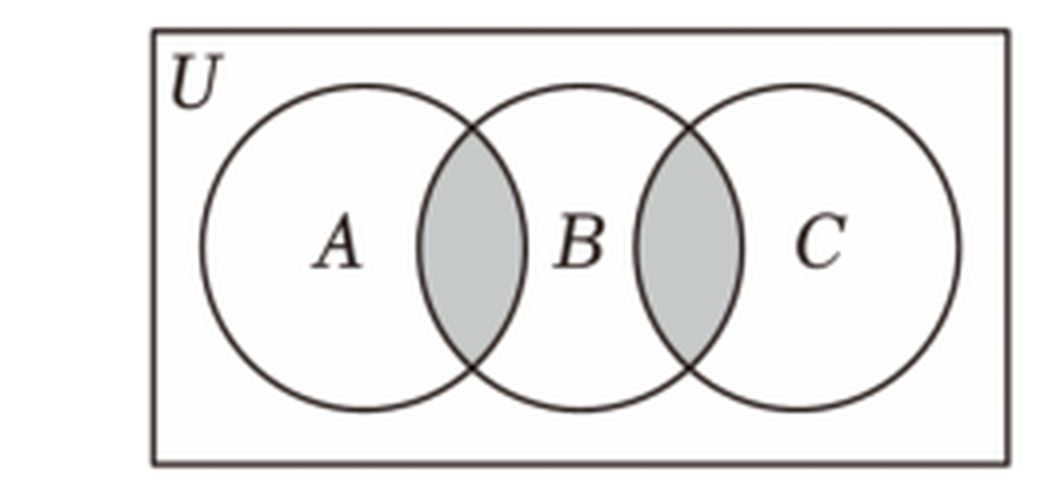
\includegraphics[width=0.30\textwidth]{figures/venn_ABC_lenses.png}
\end{center}

\keepwithprev
A. $B\cap(A\cup C)$\qquad\qquad\qquad B. $B\cap(A\cap C)$

C. $B\cap\complement_U(A\cup C)$\qquad\qquad D. $(A\cup B)\cap(B\cup C)$

\ans{$A$}

\ifanswer
\solbegin
\step{由图中阴影部分得，阴影为集合 $A$、$B$ 的交集和 $B$、$C$ 的交集的并集，}
\step{故阴影部分可表示为 $(A\cap B)\cup(B\cap C)$ 或 $B\cap(A\cup C)$，
故 $A$ 正确. 故选 $A$.}
\solend

\fi

\item 设集合 $P_1=\{x\mid x^2+ax+1>0\}$，$P_2=\{x\mid x^2+ax+2>0\}$，
$Q_1=\{x\mid x^2+x+b>0\}$，$Q_2=\{x\mid x^2+2x+b>0\}$，其中 $a$、$b\in\R$，
对于下列两个命题：①存在 $a$，$P_1$ 不是 $P_2$ 的子集；②存在 $b$ 使得 $Q_1$ 是 $Q_2$
的子集. 下列说法正确的是\mbox{（\quad）}

\keepwithprev
A. ①是真命题，②是假命题\qquad B. ①是假命题，②是真命题

C. ①②都是真命题\qquad\qquad\quad D. ①②都是假命题

\ans{$B$}

\ifanswer
\solbegin
\step{对于集合 $P_1=\{x\mid x^2+ax+1>0\}$，$P_2=\{x\mid x^2+ax+2>0\}$，}
\step{得当 $m\in P_1$ 时，即 $m^2+am+1>0$，得 $m^2+am+2>0$，}
\step{即有 $m\in P_2$，得对任意 $a$，$P_1$ 是 $P_2$ 的子集，故①错误；}
\step{对于集合 $Q_1=\{x\mid x^2+x+b>0\}$，$Q_2=\{x\mid x^2+2x+b>0\}$，}
\step{当 $b=6$ 时，$Q_1=\{x\mid x^2+x+6>0\}=\R$，$Q_2=\{x\mid x^2+2x+6>0\}=\R$，}
\step{得 $Q_1$ 是 $Q_2$ 的子集，所以存在 $b$，使得 $Q_1$ 是 $Q_2$ 的子集，故②正确；}
\step{故选 $B$.}
\solend

\fi

\item 设 $a$、$b\in\R$，则“$a+b>2$ 且 $ab>1$”是“$a>1$ 且 $b>1$”的\mbox{（\quad）}

\keepwithprev
A. 充要条件\qquad\qquad\qquad B. 充分不必要条件

C. 必要不充分条件\qquad\quad D. 既不充分又不必要条件

\ans{$C$}

\ifanswer
\solbegin
\step{因为 $a>1$ 且 $b>1$，所以 $a+b>2$ 且 $ab>1$，}
\step{若已知 $a+b>2$ 且 $ab>1$，可取 $a=\dfrac12$，$b=8$，也满足已知，}
\step{所以“$a+b>2$ 且 $ab>1$”是“$a>1$ 且 $b>1$”的必要不充分条件，故选 $C$.}
\solend

\fi

\item 十七世纪，数学家费马提出猜想：“对任意正整数 $n>2$，关于 $x$、$y$、$z$ 的方程
$x^n+y^n=z^n$ 没有正整数解”. 1995 年数学家安德鲁·怀尔斯发表了完成的证明过程，使它
终成费马大定理. 对费马大定理，若用反证法证明，第一步是假设猜想不成立，即\mbox{（\quad）}

\keepwithprev
A. 对任意正整数 $n>2$，关于 $x$、$y$、$z$ 的方程 $x^n+y^n=z^n$ 都有正整数解

B. 对任意正整数 $n>2$，关于 $x$、$y$、$z$ 的方程 $x^n+y^n=z^n$ 至少存在一组正整数解

C. 存在正整数 $n\leqslant2$，关于 $x$、$y$、$z$ 的方程 $x^n+y^n=z^n$ 至少存在一组正整数解

D. 存在正整数 $n>2$，关于 $x$、$y$、$z$ 的方程 $x^n+y^n=z^n$ 至少存在一组正整数解

\ans{$D$}

\end{enumerate}

\bigsec{三、解答题}

\begin{enumerate}
\setcounter{enumi}{16}

\item 已知 $a$、$b$、$c$ 都是实数，且 $a+b+c=0$，$abc=1$，求证：$a$、$b$、$c$ 中必有一个
大于 $\dfrac32$.

\ifanswer
\solbegin
\step{由 $a+b+c=0$，$abc=1$，得 $a$、$b$、$c$ 中一个正数，两个负数，}
\step{不妨设 $c>0$，由题意得 $a+b=-c,ab=\dfrac1c$，}
\step{由根与系数的关系得 $a$、$b$ 是关于 $x$ 的方程 $x^2+cx+\dfrac1c=0$ 的两个根，}
\step{则 $\Delta=c^2-\dfrac4c=\dfrac{c^3-4}{c}\geqslant0$，}
\step{因为 $c>0$，所以 $c^3\geqslant4$，得 $c\geqslant\sqrt[3]{4}$，}
\step{又 $\dfrac32=\sqrt[3]{\left(\dfrac32\right)^3}=\sqrt[3]{\dfrac{27}{8}}<\sqrt[3]{4}$，}
\step{所以 $c>\dfrac32$，即 $a$、$b$、$c$ 中必有一个大于 $\dfrac32$.}
\solend

\fi

\ansspace[6]

\item 已知关于 $x$ 的一元二次方程 $x^2-mx+4m^2-3=0$ 的两个实根分别为 $x_1,x_2$.

\begin{enumerate}[label=(\arabic*)]
\item $x_1,x_2$ 均为正根，求实数 $m$ 的取值范围；
\item 若 $x_1,x_2$ 满足：$x_1+x_2=x_1x_2$，求实数 $m$ 的值.
\end{enumerate}

\ifanswer
\solbegin
\stepm{(1)}{由 $x_1,x_2$ 均为正根，得}
\step{$\begin{cases}\Delta=(-m)^2-4(4m^2-3)\geqslant0\\ x_1+x_2=m>0\\ x_1\cdot x_2=4m^2-3>0\end{cases}$，}
\step{解得 $\begin{cases}-\dfrac{2\sqrt5}{5}\leqslant m\leqslant\dfrac{2\sqrt5}{5}\\[4pt]
m>0\\[4pt] m\leqslant-\dfrac{\sqrt3}{2}$ 或 $m\geqslant\dfrac{\sqrt3}{2}\end{cases}$，}
\step{即 $\dfrac{\sqrt3}{2}\leqslant m\leqslant\dfrac{2\sqrt5}{5}$；}
\stepm{(2)}{由 (1) 得
$\begin{cases}-\dfrac{2\sqrt5}{5}\leqslant m\leqslant\dfrac{2\sqrt5}{5}\\[4pt]
m=4m^2-3\end{cases}$，解得 $m=1$（舍去）或 $m=-\dfrac34$，}
\step{则 $m=-\dfrac34$.}
\solend

\fi

\ansspace[6]

\item 已知集合 $A=\{x\mid m-1<x<m^2+1\}$，$B=\{x\mid-2<x<2\}$.

\begin{enumerate}[label=(\arabic*)]
\item 当 $m=2$ 时，求 $A\cup B$、$A\cap B$、$\complement_R B$、$A\cap(\complement_R B)$；
\item 若“$x\in A$”是“$x\in B$”成立的必要不充分条件，求实数 $m$ 的取值范围.
\end{enumerate}

\ifanswer
\solbegin
\stepm{(1)}{$m=2$ 时，$A=\{x\mid1<x<5\}$，且 $B=\{x\mid-2<x<2\}$，}
\step{所以 $A\cup B=\{x\mid-2<x<5\}$，$A\cap B=\{x\mid1<x<2\}$，}
\step{$\complement_R B=\{x\mid x\leqslant-2$ 或 $x\geqslant2\}$，
$A\cap(\complement_R B)=\{x\mid2\leqslant x<5\}$；}
\stepm{(2)}{若“$x\in A$”是“$x\in B$”成立的必要不充分条件，则 $B\subset A$，}
\step{所以 $\begin{cases}m-1<-2\\ m^2+1\geqslant2\end{cases}$
或 $\begin{cases}m-1\leqslant-2\\ m^2+1>2\end{cases}$，解得 $m<-1$，}
\step{故 $m$ 的取值范围为 $(-\infty,-1)$.}
\solend

\fi

\ansspace[6]

\item 已知 $m\in\R$，集合 $A=\{x\mid|x-1|\leqslant2\}$，集合
$B=\{x\mid m-3<x\leqslant m+2\}$.

\begin{enumerate}[label=(\arabic*)]
\item 若“$x\in A$”是“$x\in B$”的充分不必要条件，求 $m$ 的取值范围；
\item 若命题“$\forall x\in B$，$x\in\complement_R A$”是真命题，求 $m$ 的取值范围；
\item 若命题“$\exists x\in A$，$x\in B$”是真命题，求 $m$ 的取值范围.
\end{enumerate}

\ifanswer
\solbegin
\stepm{(1)}{集合 $A=\{x\mid|x-1|\leqslant2\}=\{x\mid-1\leqslant x\leqslant3\}$，}
\step{若“$x\in A$”是“$x\in B$”的充分不必要条件，则 $A\subset B$，}
\step{所以 $\begin{cases}m-3<-1\\ 3\leqslant m+2\end{cases}$，解得 $1\leqslant m<2$，}
\step{当 $m=1$ 时，$B=\{x\mid-2<x\leqslant3\}$，符合题意，}
\step{所以 $m$ 的取值范围是 $\{m\mid1\leqslant m<2\}$.}
\stepm{(2)}{若命题“$\forall x\in B$，$x\in\complement_R A$”是真命题，则 $B\subset\complement_R A$，}
\step{又 $\complement_R A=\{x\mid x<-1$ 或 $x>3\}$，$B\neq\varnothing$，
所以 $m+2<-1$ 或 $m-3\geqslant3$，}
\step{解得 $m<-3$ 或 $m\geqslant6$，所以 $\{m\mid m<-3$ 或 $m\geqslant6\}$；}
\stepm{(3)}{因为 $\exists x\in A$，$x\in B$ 是真命题，所以 $A\cap B\neq\varnothing$，}
\step{当 $A\cap B=\varnothing$ 时，所以 $m+2<-1$ 或 $m-3\geqslant3$，
即 $m<-3$ 或 $m\geqslant6$，}
\step{所以当 $A\cap B\neq\varnothing$ 时，$m$ 的取值范围是 $\{m\mid-3\leqslant m<6\}$，}
\step{则 $m$ 的取值范围是 $\{m\mid-3\leqslant m<6\}$.}
\solend

\fi

\ansspace[6]

\item 对于函数 $f(x)$，若 $f(x_0)=x_0$，则称 $x_0$ 为 $f(x)$ 的“不动点”；若
$f[f(x_0)]=x_0$，则称 $x_0$ 为 $f(x)$ 的“稳定点”. 函数 $f(x)$ 的“不动点”和“稳定点”
的集合分别记为 $A$ 和 $B$，即 $A=\{x\mid f(x)=x\}$，$B=\{x\mid f[f(x)]=x\}$.

\begin{enumerate}[label=(\arabic*)]
\item 设函数 $f(x)=3x+4$，求集合 $A$ 和 $B$；
\item 求证：$A\sub B$；
\item 设函数 $f(x)=ax^2+bx+c(a\neq0)$，且 $A=\varnothing$，求证：$B=\varnothing$.
\end{enumerate}

\ifanswer
\solbegin
\stepm{(1)}{令 $f(x)=3x+4=x$，解得 $x=-2$，故有 $A=\{-2\}$，}
\step{由于 $f[f(x)]=3(3x+4)+4=9x+16$，}
\step{令 $9x+16=x$，得 $x=-2$，故有 $B=\{-2\}$；}
\stepm{(2)}{若 $A=\varnothing$，则 $A\sub B$ 显然成立；}
\step{若 $A\neq\varnothing$，设 $t\in A$，则 $f(t)=t$，$f(f(t))=f(t)=t$，}
\step{所以 $t\in B$，故 $A\sub B$.}
\stepm{(3)}{因为 $A=\{x\mid f(x)=x\}=\varnothing$，所以 $ax^2+bx+c=x$ 无解，}
\step{即 $\Delta=(b-1)^2-4a<0$，}
\step{①当 $a>0$ 时，二次函数 $y=f(x)-x$，}
\step{即 $y=ax^2+(b-1)x+c$ 的图象在 $x$ 轴的上方，}
\step{所以 $\forall x\in\R$，$f(x)-x>0$ 恒成立，所以 $\forall x\in\R$，
$f(x)>x$ 恒成立，}
\step{所以 $\forall x\in\R$，$f[f(x)]>f(x)>x$ 恒成立，即 $B=\varnothing$；}
\step{②当 $a<0$ 时，同理可证 $B=\varnothing$；}
\step{综上，对于函数 $f(x)=ax^2+bx+c(a\neq0)$，当 $A=\varnothing$ 时，$B=\varnothing$.}
\solend

\fi

\ansspace*[10]

\end{enumerate}

\end{document}
"
% 紧凑版：xelatex "\def\iscompact{1}% 高一26_交附闵行_周练2.tex
%   —— 高一上数学「2026-2027 年交附闵行高一上周练 2」（试卷版/答案版）
% 试卷版：xelatex 高一26_交附闵行_周练2.tex
% 答案版：xelatex "\def\isanswer{1}\input{高一26_交附闵行_周练2.tex}"
% 紧凑版：xelatex "\def\iscompact{1}\input{高一26_交附闵行_周练2.tex}"
%
% 原始材料是微信公众号图文（公众号「魔都数学加油站」连载「27学年高一 26」，2026-09-21 发布，
% 原文标题「27学年高一26——2026-2027年上海市交附闵行高一上周练2」），
% 正文为 10 张 PNG 页（1080×1527，各页同尺寸）。原文本身就是一份**讲评版**——
% 题目下方直接印出【解析】（本卷无单独的【答案】行，填空题答案都写在解析里）。
% 试题文字与解析均照原卷录入，未改内容。卷面的粉色斜水印「魔都数学加油站」属水印，未录入。
%
% 卷首标题：原卷印作「2026-2027 年交附闵行高一上周练 2」（公众号标题里的「上海市」
% 三字卷面标题行没有，本稿照卷面），年份区间按全稿惯例排 en dash，前缀照原卷保留「年」。
%
% 与原卷的排版差异（均已在 README「说明」中交代）：
%   ① 原文自**第 3 题**起（第 1、2 题未在该文中发布），故本稿题号亦自 3 起；
%   ② 原卷本就印有「一、填空题」「二、选择题」「三、解答题」三节标题，本稿照原卷分节，
%      只把标题改排成全稿统一的「大节标题」样式；
%   ③ 原卷第 16 题的答案「D」直接印在题干末尾的括号内（原卷把括号连同 D 单独占一行），
%      第 13—15 题的括号空着、答案写在解析末句「故选 A／B／C」里；填空题的答案也都嵌在
%      解析里，本稿统一改为试卷版隐去、答案版以 \ans{} 给出（选择题另附【解析】）；
%   ④ 子集符号原卷两种并用：第 4 题题干与第 8 题、第 21(2) 题等作带下划线的 $\subseteq$，
%      第 19(2)、20(1)(2) 题作真包含的 $\subset$，本稿分别照录为 $\sub$ 与 $\subset$；
%   ⑤ 补集符号原卷作 $\complement_R$、$\complement_U$（第 4 题命题④、第 13 题选项 C、
%      第 19—20 题），本稿照录；
%   ⑥ 原卷的实数集 R 一律作斜体（第 11 题「$a\in R$」、第 14 题「$a$、$b\in R$」与解析的
%      $\{x\mid x^2+x+6>0\}=R$ 等），本稿按全稿惯例统一写作 $\R$；
%   ⑦ 原卷填空的横线约两个字宽，本稿按全稿惯例统一排 \blankline[4.4em]；
%   ⑧ 原卷未印副标题，本稿按全稿惯例补出副标题「集合与常用逻辑用语」；
%   ⑨ 第 13 题的 Venn 图原卷印在题干右侧（第 5 页），本稿移至题干之后；
%      图取原卷截图、4× LANCZOS 放大（figures/venn_ABC_lenses.png，
%      阴影为 $A\cap B$ 与 $B\cap C$ 两个交带，即 $(A\cap B)\cup(B\cap C)$）。
%
% 原卷存疑一处（照抄原卷、未改，见源码中该处上方注释）：
%   ① 第 12 题【解析】首步的方程组里印 $t<2$，而其后三处与末行答案都作 $t\leqslant2$
%      （$\left[\dfrac85,\dfrac{17}{10}\right)\cup\left(\dfrac95,2\right]$ 含 $2$）——
%      按题意 $N=\left\{x\mid t-\dfrac35\leqslant x\leqslant t\right\}\sub\{x\mid1\leqslant x\leqslant2\}$
%      只要求 $t\leqslant2$（$t=2$ 时 $N=\left[\dfrac75,2\right]$ 确实含于其中），
%      故方程组里的 $t<2$ 应是原卷笔误；本稿两处都照原卷录入、未互相迁就。
% 另：第 20(3) 题解析末两行原卷即作同话重复，照原卷录入。

\documentclass[a4paper,11pt]{article}
\usepackage{common}

\begin{document}

\examtitlest[3]{2026--2027 年交附闵行高一上周练 2}{集合与常用逻辑用语}

\bigsec{一、填空题}

\begin{enumerate}
\setcounter{enumi}{2}

\item 命题甲：集合 $M=\{x\mid kx^2-2kx+1=0\}$ 为空集；命题乙：关于 $x$ 的不等式
$x^2+(k-1)x+4>0$ 的解集为 $\R$. 若命题甲、乙中有且只有一个是真命题，则实数 $k$ 的取
值范围是 \blankline[4.4em].

\ifanswer
\solbegin
\step{因为集合 $M=\{x\mid kx^2-2kx+1=0\}$ 为空集，}
\step{当 $k\neq0$ 时，$\Delta=(-2k)^2-4k<0$，解得 $0<k<1$，}
\step{当 $k=0$ 时，方程变为 $1=0$，无解，满足题意，故 $0\leqslant k<1$；}
\step{又关于 $x$ 的不等式 $x^2+(k-1)x+4>0$ 的解集为 $\R$，}
\step{所以 $\Delta'=(k-1)^2-4\times4<0$，解得 $-3<k<5$，}
\step{当甲命题为真，乙命题为假时，无解，}
\step{当甲命题为假，乙命题为真时，$k\in(-3,0)\cup[1,5)$.}
\solend

\fi

\item 对任意 $A$、$B\sub\R$，记 $A\oplus B=\{x\mid x\in A\cup B,x\notin A\cap B\}$，
并称 $A\oplus B$ 为集合 $A$、$B$ 的对称差. 例如：若 $A=\{1,2,3\},B=\{2,3,4\}$，
则 $A\oplus B=\{1,4\}$. 下列命题中，为真命题的是 \blankline[4.4em].

\keepwithprev
①若 $A$、$B\sub\R$ 且 $A\oplus B\sub A$，则 $A\sub B$

②若 $A$、$B\sub\R$ 且 $A\oplus B=\varnothing$，则 $A=B$

③若 $A$、$B\sub\R$ 且 $A\oplus B=B$，则 $A=\varnothing$

④对任意 $A$、$B\sub\R$，都有 $A\oplus B=\complement_R A\oplus\complement_R B$

\ans{②③④}

\ifanswer
\solbegin
\step{对于①，因为 $A\oplus B\sub A$，
所以 $\{x\mid x\in A\cup B,x\notin A\cap B\}\sub A$，}
\step{故 $B\sub A$，①错误；}
\step{对于②，$A$、$B\sub\R$ 且 $A\oplus B=\varnothing$，
则 $\varnothing=\{x\mid x\in A\cup B,x\notin A\cap B\}$，}
\step{即 $A\cup B=A\cap B$，所以 $A=B$，②正确；}
\step{对于③，$A$、$B\sub\R$ 且 $A\oplus B=B$，
则 $B=\{x\mid x\in A\cup B,x\notin A\cap B\}$，}
\step{故 $A\sub B$，且 $B$ 中元素不在 $A\cap B$ 中，故 $A=\varnothing$，③正确；}
\step{对于④，$\complement_R A\oplus\complement_R B
=\{x\mid x\in\complement_R A\cup\complement_R B,x\notin\complement_R A\cap\complement_R B\}$，}
\step{其中 $\complement_R A\cup\complement_R B=\complement_R(A\cap B)$，
$\complement_R A\cap\complement_R B=\complement_R(A\cup B)$，}
\step{故 $\complement_R A\oplus\complement_R B
=\{x\mid x\in\complement_R(A\cap B),x\notin\complement_R(A\cup B)\}
=\{x\mid x\in A\cup B,x\notin A\cap B\}$，}
\step{而 $A\oplus B=\{x\mid x\in A\cup B,x\notin A\cap B\}$，
故 $A\oplus B=\complement_R A\oplus\complement_R B$，④正确.}
\step{故正确的是②③④.}
\solend

\fi

\item 已知 $A=\{a_1,a_2,a_3,a_4\},B=\{a^2\mid a\in A\}$，其中 $a_1<a_2<a_3<a_4$，
且 $a_1$、$a_2$、$a_3$、$a_4$ 均为整数，若 $A\cap B=\{a_3,a_4\},a_1+a_3=0$，
且 $A\cup B$ 中的所有元素之和为 $270$，则集合 $A$ 中所有元素之和为 \blankline[4.4em].

\ifanswer
\solbegin
\step{$A=\{a_1,a_2,a_3,a_4\},B=\{a^2\mid a\in A\}$，
因为 $A\cap B=\{a_3,a_4\},a_1+a_3=0$，}
\step{所以 $A=\{a_1,a_2,a_3,a_4\},B=\left\{a_1^2,a_2^2,a_4^2\right\}$，}
\step{若 $a_1^2=a_3$，则 $a_1=-1,a_3=1$，则 $a_2=0$，
此时 $A=\{-1,0,1,a_4\},B=\{0,1,a_4^2\}$，}
\step{因为 $A\cup B$ 中的所有元素之和为 $270$，
所以 $-1+0+1+a_4+1+a_4^2=270$，}
\step{无正整数解，舍去；}
\step{若 $a_2^2=a_3$，① $a_4^2=a_4$，所以 $a_4=1$，矛盾；}
\step{② $a_1^2=a_4$，此时 $A\cup B=\left\{-a_2^2,a_2,a_2^2,a_1^2,a_4^2\right\}$，
所以 $a_2^8+a_2^4+a_2=270$，}
\step{所以 $a_2=-2$，此时 $a_1=-4,a_2=-2,a_3=4,a_4=16$；}
\step{若 $a_4^2=a_3$，显然不成立；}
\step{综上，集合 $A$ 中所有元素之和为 $-4-2+4+16=14$.}
\solend

\fi

\item 将集合 $M=\{a_1,a_2,a_3,\cdots,a_n\}$ 分拆成两个集合 $A_i$ 和 $B_j$，且
$M\supseteq A_i\cup B_j$，$A_i\cap B_j=\varnothing$，这样的分拆方法共有 \blankline[4.4em] 种.

\ifanswer
\solbegin
\step{按集合 $A_i$ 中的元素个数进行分类：}
\step{若 $A_i$ 中有 $0$ 个元素（即 $C_n^0$ 种）时，则 $B_j$ 有 $2^n$ 种，
共有 $2^nC_n^0$ 种；}
\step{若 $A_i$ 中有 $1$ 个元素（即 $C_n^1$ 种）时，则 $B_j$ 有 $2^{n-1}$ 种，
共有 $2^{n-1}C_n^1$ 种；}
\step{若 $A_i$ 中有 $2$ 个元素（即 $C_n^2$ 种）时，则 $B_j$ 有 $2^{n-2}$ 种，
共有 $2^{n-2}C_n^2$ 种；}
\step{若 $A_i$ 中有 $3$ 个元素（即 $C_n^3$ 种）时，则 $B_j$ 有 $2^{n-3}$ 种，
共有 $2^{n-3}C_n^3$ 种；}
\step{若 $A_i$ 中有 $n$ 个元素（即 $C_n^n$ 种）时，则 $B_j$ 有 $2^0$ 种，
共有 $2^0C_n^n$ 种；}
\step{得 $2^nC_n^0+2^{n-1}C_n^1+2^{n-2}C_n^2+\cdots+2^0C_n^n=(1+2)^n$，
故这样的分拆方法有 $3^n$ 种.}
\solend

\fi

\item 已知集合 $A=\{x\mid x<2,x\in\Z\}$，$B=\{x\mid x>0,x\in\Z\}$，则
$A\cap B=$ \blankline[4.4em].

\ifanswer
\solbegin
\step{因为 $A=\{x\mid x<2,x\in\Z\}$，$B=\{x\mid x>0,x\in\Z\}$，}
\step{所以 $A\cap B=\{x\mid0<x<2,x\in\Z\}=\{1\}$.}
\solend

\fi

\item 已知集合 $A=\{x\mid(a-1)x^2+3x-2=0\}$，$B=\{x\mid x^2-3x+2=0\}$，若
$A\sub B$，求实数 $a$ 的取值范围是 \blankline[4.4em].

\ifanswer
\solbegin
\step{由方程 $x^2-3x+2=0$，解得 $x=1$ 或 $x=2$，即 $B=\{1,2\}$，}
\step{因为 $A\sub B$，所以 $A=\varnothing$ 或 $A=\{1\}$ 或 $A=\{2\}$ 或 $A=\{1,2\}$，}
\step{当 $A=\varnothing$ 时，
则 $\begin{cases}a\neq1\\ \Delta=3^2-4(a-1)\times(-2)<0\end{cases}$，
解得 $a<-\dfrac18$；}
\step{将 $x=1$ 代入方程 $(a-1)x^2+3x-2=0$，得 $a=0$，}
\step{此时 $A=\{x\mid-x^2+3x-2=0\}=\{1,2\}$，满足条件；}
\step{将 $x=2$ 代入方程 $(a-1)x^2+3x-2=0$，得到 $a=0$，上面已经验证满足条件；}
\step{综上所述，$a$ 的取值范围是 $\left(-\infty,-\dfrac18\right)\cup\{0\}$.}
\solend

\fi

\item 已知方程 $x^2-3x+a=0$ 的两根都大于 $1$，则 $a$ 的取值范围为 \blankline[4.4em].

\ifanswer
\solbegin
\step{由题意得 $\Delta=9-4a\geqslant0$，$x_1+x_2=3$，$x_1x_2=a$，
所以 $a\leqslant\dfrac94$，}
\step{则 $(x_1-1)(x_2-1)=x_1x_2-(x_1+x_2)+1=a-3+1>0$，所以 $a>2$，}
\step{故 $a$ 的范围为 $\left(2,\dfrac94\right]$.}
\solend

\fi

\item 设 $x_1$、$x_2$ 是方程 $x^2+x-3=0$ 的两个实数根，则 $x_1^2-x_2+2024=$
\blankline[4.4em].

\ifanswer
\solbegin
\step{由题意得 $x_1^2=3-x_1$，$x_1+x_2=-1$，}
\step{则 $x_1^2-x_2+2024=3-x_1-x_2+2024=2027-(-1)=2028$.}
\solend

\fi

\item 已知 $a\in\R$，若关于 $x$ 的方程 $x^2+ax+a^2-8=0$ 有两个实根 $x_1$、$x_2$，且
$\dfrac1{x_1}+\dfrac1{x_2}=-\dfrac12$，则 $a$ 的值为 \blankline[4.4em].

\ifanswer
\solbegin
\step{由题意得 $\Delta=a^2-4(a^2-8)=32-3a^2\geqslant0$，
解得 $a^2\leqslant\dfrac{32}{3}$，}
\step{由韦达定理得 $x_1+x_2=-a$，$x_1x_2=a^2-8$，}
\step{则 $\dfrac1{x_1}+\dfrac1{x_2}=\dfrac{x_1+x_2}{x_1x_2}
=\dfrac{-a}{a^2-8}=-\dfrac12$，}
\step{即 $a^2-2a-8=(a-4)(a+2)=0$，解得 $a=4$ 或 $a=-2$.}
\step{又 $a^2\leqslant\dfrac{32}{3}$，则 $a=-2$.}
\solend

\fi

\item 定义集合 $P=\{x\mid a\leqslant x\leqslant b\}$ 的“长度”是 $b-a$，其中 $a$、
$b\in\R$. 已知集合 $M=\left\{x\mid\dfrac65\leqslant x\leqslant\dfrac{17}{10}\right\}$，
$N=\left\{x\mid t-\dfrac35\leqslant x\leqslant t\right\}$，且 $M$、$N$ 都是集合
$\{x\mid1\leqslant x\leqslant2\}$ 的子集，若集合 $M\cup N$ 的“长度”大于 $\dfrac35$，
则 $t$ 的取值范围是 \blankline[4.4em].

\ifanswer
\solbegin
\step{因为 $N=\left\{x\mid t-\dfrac35\leqslant x\leqslant t\right\}$
是集合 $\{x\mid1\leqslant x\leqslant2\}$ 的子集，}
% 注：下一行方程组里的 $t<2$ 系原卷所印（本稿照录），与其后三处及末行答案的
%     $t\leqslant2$ 自相矛盾——按题意应为 $t\leqslant2$，见文件头「原卷存疑」①。
\step{所以 $\begin{cases}t-\dfrac35\geqslant1\\[2pt] t<2\end{cases}$，
解得 $\dfrac85\leqslant t\leqslant2$，}
\step{又 $M=\left\{x\mid\dfrac65\leqslant x\leqslant\dfrac{17}{10}\right\}$，
得集合 $M$ 的“长度”为 $\dfrac{17}{10}-\dfrac65=\dfrac12$，}
\step{又 $N=\left\{x\mid t-\dfrac35\leqslant x\leqslant t\right\}$，
要使集合 $M\cup N$ 的“长度”大于 $\dfrac35$，}
\step{若 $M\cup N=\left\{x\mid t-\dfrac35\leqslant x\leqslant\dfrac{17}{10}\right\}$，
则 $\dfrac{17}{10}-t+\dfrac35>\dfrac35$，所以 $t<\dfrac{17}{10}$，}
\step{又 $\dfrac85\leqslant t\leqslant2$，所以 $\dfrac85\leqslant t<\dfrac{17}{10}$；}
\step{若 $M\cup N=\left\{x\mid\dfrac65\leqslant x\leqslant t\right\}$，
则 $t-\dfrac65>\dfrac35$，所以 $t>\dfrac95$，}
\step{又 $\dfrac85\leqslant t\leqslant2$，所以 $\dfrac95<t\leqslant2$；}
\step{则 $t$ 的取值范围是 $\left[\dfrac85,\dfrac{17}{10}\right)\cup\left(\dfrac95,2\right]$.}
\solend

\fi

\end{enumerate}

% 第 13 题是「题干 + 图 + 选项」约 5.7cm 的一整块（图 0.30\textwidth、宽高比 0.477 → 高 2.29cm，
% 加题干 1 行、选项 2 行与段间距）。`\keepwithprev` 只挡得住「题干—选项」之间，挡不住
% 夹在中间的图——实测断点落在题干之后，题干孤零零留在 p1、图与四个选项整页翻到 p2
% （切页审计的 A 类）。故照 高一30 第 4 题的成例先量一次页高；**守卫要放在 `\bigsec` 之前**
% 连节标题一起量（放标题之后会把「二、选择题」孤立在页末，正是 高一40 修过的那类 B 类）。
% 7cm ＝ 节标题约 1.1cm ＋ 第 13 题那块约 5.7cm（留少量余量）。
\needvspace{7cm}
\bigsec{二、选择题}

\begin{enumerate}
\setcounter{enumi}{12}

\item 图中阴影部分用集合符号可以表示为\mbox{（\quad）}

\begin{center}
% 图取原卷截图、4× LANCZOS 放大（原卷把图印在题干右侧，本稿移至此处，见文件头⑨）。
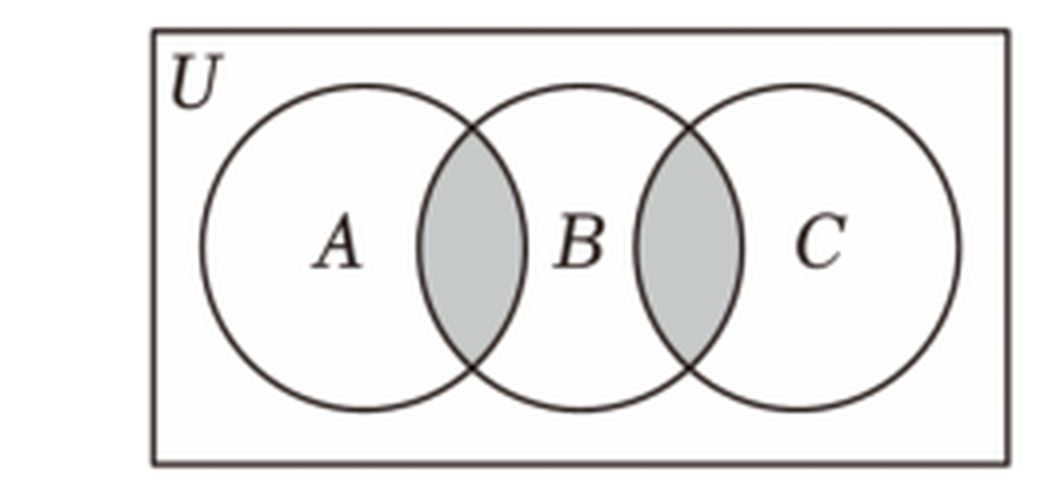
\includegraphics[width=0.30\textwidth]{figures/venn_ABC_lenses.png}
\end{center}

\keepwithprev
A. $B\cap(A\cup C)$\qquad\qquad\qquad B. $B\cap(A\cap C)$

C. $B\cap\complement_U(A\cup C)$\qquad\qquad D. $(A\cup B)\cap(B\cup C)$

\ans{$A$}

\ifanswer
\solbegin
\step{由图中阴影部分得，阴影为集合 $A$、$B$ 的交集和 $B$、$C$ 的交集的并集，}
\step{故阴影部分可表示为 $(A\cap B)\cup(B\cap C)$ 或 $B\cap(A\cup C)$，
故 $A$ 正确. 故选 $A$.}
\solend

\fi

\item 设集合 $P_1=\{x\mid x^2+ax+1>0\}$，$P_2=\{x\mid x^2+ax+2>0\}$，
$Q_1=\{x\mid x^2+x+b>0\}$，$Q_2=\{x\mid x^2+2x+b>0\}$，其中 $a$、$b\in\R$，
对于下列两个命题：①存在 $a$，$P_1$ 不是 $P_2$ 的子集；②存在 $b$ 使得 $Q_1$ 是 $Q_2$
的子集. 下列说法正确的是\mbox{（\quad）}

\keepwithprev
A. ①是真命题，②是假命题\qquad B. ①是假命题，②是真命题

C. ①②都是真命题\qquad\qquad\quad D. ①②都是假命题

\ans{$B$}

\ifanswer
\solbegin
\step{对于集合 $P_1=\{x\mid x^2+ax+1>0\}$，$P_2=\{x\mid x^2+ax+2>0\}$，}
\step{得当 $m\in P_1$ 时，即 $m^2+am+1>0$，得 $m^2+am+2>0$，}
\step{即有 $m\in P_2$，得对任意 $a$，$P_1$ 是 $P_2$ 的子集，故①错误；}
\step{对于集合 $Q_1=\{x\mid x^2+x+b>0\}$，$Q_2=\{x\mid x^2+2x+b>0\}$，}
\step{当 $b=6$ 时，$Q_1=\{x\mid x^2+x+6>0\}=\R$，$Q_2=\{x\mid x^2+2x+6>0\}=\R$，}
\step{得 $Q_1$ 是 $Q_2$ 的子集，所以存在 $b$，使得 $Q_1$ 是 $Q_2$ 的子集，故②正确；}
\step{故选 $B$.}
\solend

\fi

\item 设 $a$、$b\in\R$，则“$a+b>2$ 且 $ab>1$”是“$a>1$ 且 $b>1$”的\mbox{（\quad）}

\keepwithprev
A. 充要条件\qquad\qquad\qquad B. 充分不必要条件

C. 必要不充分条件\qquad\quad D. 既不充分又不必要条件

\ans{$C$}

\ifanswer
\solbegin
\step{因为 $a>1$ 且 $b>1$，所以 $a+b>2$ 且 $ab>1$，}
\step{若已知 $a+b>2$ 且 $ab>1$，可取 $a=\dfrac12$，$b=8$，也满足已知，}
\step{所以“$a+b>2$ 且 $ab>1$”是“$a>1$ 且 $b>1$”的必要不充分条件，故选 $C$.}
\solend

\fi

\item 十七世纪，数学家费马提出猜想：“对任意正整数 $n>2$，关于 $x$、$y$、$z$ 的方程
$x^n+y^n=z^n$ 没有正整数解”. 1995 年数学家安德鲁·怀尔斯发表了完成的证明过程，使它
终成费马大定理. 对费马大定理，若用反证法证明，第一步是假设猜想不成立，即\mbox{（\quad）}

\keepwithprev
A. 对任意正整数 $n>2$，关于 $x$、$y$、$z$ 的方程 $x^n+y^n=z^n$ 都有正整数解

B. 对任意正整数 $n>2$，关于 $x$、$y$、$z$ 的方程 $x^n+y^n=z^n$ 至少存在一组正整数解

C. 存在正整数 $n\leqslant2$，关于 $x$、$y$、$z$ 的方程 $x^n+y^n=z^n$ 至少存在一组正整数解

D. 存在正整数 $n>2$，关于 $x$、$y$、$z$ 的方程 $x^n+y^n=z^n$ 至少存在一组正整数解

\ans{$D$}

\end{enumerate}

\bigsec{三、解答题}

\begin{enumerate}
\setcounter{enumi}{16}

\item 已知 $a$、$b$、$c$ 都是实数，且 $a+b+c=0$，$abc=1$，求证：$a$、$b$、$c$ 中必有一个
大于 $\dfrac32$.

\ifanswer
\solbegin
\step{由 $a+b+c=0$，$abc=1$，得 $a$、$b$、$c$ 中一个正数，两个负数，}
\step{不妨设 $c>0$，由题意得 $a+b=-c,ab=\dfrac1c$，}
\step{由根与系数的关系得 $a$、$b$ 是关于 $x$ 的方程 $x^2+cx+\dfrac1c=0$ 的两个根，}
\step{则 $\Delta=c^2-\dfrac4c=\dfrac{c^3-4}{c}\geqslant0$，}
\step{因为 $c>0$，所以 $c^3\geqslant4$，得 $c\geqslant\sqrt[3]{4}$，}
\step{又 $\dfrac32=\sqrt[3]{\left(\dfrac32\right)^3}=\sqrt[3]{\dfrac{27}{8}}<\sqrt[3]{4}$，}
\step{所以 $c>\dfrac32$，即 $a$、$b$、$c$ 中必有一个大于 $\dfrac32$.}
\solend

\fi

\ansspace[6]

\item 已知关于 $x$ 的一元二次方程 $x^2-mx+4m^2-3=0$ 的两个实根分别为 $x_1,x_2$.

\begin{enumerate}[label=(\arabic*)]
\item $x_1,x_2$ 均为正根，求实数 $m$ 的取值范围；
\item 若 $x_1,x_2$ 满足：$x_1+x_2=x_1x_2$，求实数 $m$ 的值.
\end{enumerate}

\ifanswer
\solbegin
\stepm{(1)}{由 $x_1,x_2$ 均为正根，得}
\step{$\begin{cases}\Delta=(-m)^2-4(4m^2-3)\geqslant0\\ x_1+x_2=m>0\\ x_1\cdot x_2=4m^2-3>0\end{cases}$，}
\step{解得 $\begin{cases}-\dfrac{2\sqrt5}{5}\leqslant m\leqslant\dfrac{2\sqrt5}{5}\\[4pt]
m>0\\[4pt] m\leqslant-\dfrac{\sqrt3}{2}$ 或 $m\geqslant\dfrac{\sqrt3}{2}\end{cases}$，}
\step{即 $\dfrac{\sqrt3}{2}\leqslant m\leqslant\dfrac{2\sqrt5}{5}$；}
\stepm{(2)}{由 (1) 得
$\begin{cases}-\dfrac{2\sqrt5}{5}\leqslant m\leqslant\dfrac{2\sqrt5}{5}\\[4pt]
m=4m^2-3\end{cases}$，解得 $m=1$（舍去）或 $m=-\dfrac34$，}
\step{则 $m=-\dfrac34$.}
\solend

\fi

\ansspace[6]

\item 已知集合 $A=\{x\mid m-1<x<m^2+1\}$，$B=\{x\mid-2<x<2\}$.

\begin{enumerate}[label=(\arabic*)]
\item 当 $m=2$ 时，求 $A\cup B$、$A\cap B$、$\complement_R B$、$A\cap(\complement_R B)$；
\item 若“$x\in A$”是“$x\in B$”成立的必要不充分条件，求实数 $m$ 的取值范围.
\end{enumerate}

\ifanswer
\solbegin
\stepm{(1)}{$m=2$ 时，$A=\{x\mid1<x<5\}$，且 $B=\{x\mid-2<x<2\}$，}
\step{所以 $A\cup B=\{x\mid-2<x<5\}$，$A\cap B=\{x\mid1<x<2\}$，}
\step{$\complement_R B=\{x\mid x\leqslant-2$ 或 $x\geqslant2\}$，
$A\cap(\complement_R B)=\{x\mid2\leqslant x<5\}$；}
\stepm{(2)}{若“$x\in A$”是“$x\in B$”成立的必要不充分条件，则 $B\subset A$，}
\step{所以 $\begin{cases}m-1<-2\\ m^2+1\geqslant2\end{cases}$
或 $\begin{cases}m-1\leqslant-2\\ m^2+1>2\end{cases}$，解得 $m<-1$，}
\step{故 $m$ 的取值范围为 $(-\infty,-1)$.}
\solend

\fi

\ansspace[6]

\item 已知 $m\in\R$，集合 $A=\{x\mid|x-1|\leqslant2\}$，集合
$B=\{x\mid m-3<x\leqslant m+2\}$.

\begin{enumerate}[label=(\arabic*)]
\item 若“$x\in A$”是“$x\in B$”的充分不必要条件，求 $m$ 的取值范围；
\item 若命题“$\forall x\in B$，$x\in\complement_R A$”是真命题，求 $m$ 的取值范围；
\item 若命题“$\exists x\in A$，$x\in B$”是真命题，求 $m$ 的取值范围.
\end{enumerate}

\ifanswer
\solbegin
\stepm{(1)}{集合 $A=\{x\mid|x-1|\leqslant2\}=\{x\mid-1\leqslant x\leqslant3\}$，}
\step{若“$x\in A$”是“$x\in B$”的充分不必要条件，则 $A\subset B$，}
\step{所以 $\begin{cases}m-3<-1\\ 3\leqslant m+2\end{cases}$，解得 $1\leqslant m<2$，}
\step{当 $m=1$ 时，$B=\{x\mid-2<x\leqslant3\}$，符合题意，}
\step{所以 $m$ 的取值范围是 $\{m\mid1\leqslant m<2\}$.}
\stepm{(2)}{若命题“$\forall x\in B$，$x\in\complement_R A$”是真命题，则 $B\subset\complement_R A$，}
\step{又 $\complement_R A=\{x\mid x<-1$ 或 $x>3\}$，$B\neq\varnothing$，
所以 $m+2<-1$ 或 $m-3\geqslant3$，}
\step{解得 $m<-3$ 或 $m\geqslant6$，所以 $\{m\mid m<-3$ 或 $m\geqslant6\}$；}
\stepm{(3)}{因为 $\exists x\in A$，$x\in B$ 是真命题，所以 $A\cap B\neq\varnothing$，}
\step{当 $A\cap B=\varnothing$ 时，所以 $m+2<-1$ 或 $m-3\geqslant3$，
即 $m<-3$ 或 $m\geqslant6$，}
\step{所以当 $A\cap B\neq\varnothing$ 时，$m$ 的取值范围是 $\{m\mid-3\leqslant m<6\}$，}
\step{则 $m$ 的取值范围是 $\{m\mid-3\leqslant m<6\}$.}
\solend

\fi

\ansspace[6]

\item 对于函数 $f(x)$，若 $f(x_0)=x_0$，则称 $x_0$ 为 $f(x)$ 的“不动点”；若
$f[f(x_0)]=x_0$，则称 $x_0$ 为 $f(x)$ 的“稳定点”. 函数 $f(x)$ 的“不动点”和“稳定点”
的集合分别记为 $A$ 和 $B$，即 $A=\{x\mid f(x)=x\}$，$B=\{x\mid f[f(x)]=x\}$.

\begin{enumerate}[label=(\arabic*)]
\item 设函数 $f(x)=3x+4$，求集合 $A$ 和 $B$；
\item 求证：$A\sub B$；
\item 设函数 $f(x)=ax^2+bx+c(a\neq0)$，且 $A=\varnothing$，求证：$B=\varnothing$.
\end{enumerate}

\ifanswer
\solbegin
\stepm{(1)}{令 $f(x)=3x+4=x$，解得 $x=-2$，故有 $A=\{-2\}$，}
\step{由于 $f[f(x)]=3(3x+4)+4=9x+16$，}
\step{令 $9x+16=x$，得 $x=-2$，故有 $B=\{-2\}$；}
\stepm{(2)}{若 $A=\varnothing$，则 $A\sub B$ 显然成立；}
\step{若 $A\neq\varnothing$，设 $t\in A$，则 $f(t)=t$，$f(f(t))=f(t)=t$，}
\step{所以 $t\in B$，故 $A\sub B$.}
\stepm{(3)}{因为 $A=\{x\mid f(x)=x\}=\varnothing$，所以 $ax^2+bx+c=x$ 无解，}
\step{即 $\Delta=(b-1)^2-4a<0$，}
\step{①当 $a>0$ 时，二次函数 $y=f(x)-x$，}
\step{即 $y=ax^2+(b-1)x+c$ 的图象在 $x$ 轴的上方，}
\step{所以 $\forall x\in\R$，$f(x)-x>0$ 恒成立，所以 $\forall x\in\R$，
$f(x)>x$ 恒成立，}
\step{所以 $\forall x\in\R$，$f[f(x)]>f(x)>x$ 恒成立，即 $B=\varnothing$；}
\step{②当 $a<0$ 时，同理可证 $B=\varnothing$；}
\step{综上，对于函数 $f(x)=ax^2+bx+c(a\neq0)$，当 $A=\varnothing$ 时，$B=\varnothing$.}
\solend

\fi

\ansspace*[10]

\end{enumerate}

\end{document}
"
%
% 原始材料是微信公众号图文（公众号「魔都数学加油站」连载「27学年高一 26」，2026-09-21 发布，
% 原文标题「27学年高一26——2026-2027年上海市交附闵行高一上周练2」），
% 正文为 10 张 PNG 页（1080×1527，各页同尺寸）。原文本身就是一份**讲评版**——
% 题目下方直接印出【解析】（本卷无单独的【答案】行，填空题答案都写在解析里）。
% 试题文字与解析均照原卷录入，未改内容。卷面的粉色斜水印「魔都数学加油站」属水印，未录入。
%
% 卷首标题：原卷印作「2026-2027 年交附闵行高一上周练 2」（公众号标题里的「上海市」
% 三字卷面标题行没有，本稿照卷面），年份区间按全稿惯例排 en dash，前缀照原卷保留「年」。
%
% 与原卷的排版差异（均已在 README「说明」中交代）：
%   ① 原文自**第 3 题**起（第 1、2 题未在该文中发布），故本稿题号亦自 3 起；
%   ② 原卷本就印有「一、填空题」「二、选择题」「三、解答题」三节标题，本稿照原卷分节，
%      只把标题改排成全稿统一的「大节标题」样式；
%   ③ 原卷第 16 题的答案「D」直接印在题干末尾的括号内（原卷把括号连同 D 单独占一行），
%      第 13—15 题的括号空着、答案写在解析末句「故选 A／B／C」里；填空题的答案也都嵌在
%      解析里，本稿统一改为试卷版隐去、答案版以 \ans{} 给出（选择题另附【解析】）；
%   ④ 子集符号原卷两种并用：第 4 题题干与第 8 题、第 21(2) 题等作带下划线的 $\subseteq$，
%      第 19(2)、20(1)(2) 题作真包含的 $\subset$，本稿分别照录为 $\sub$ 与 $\subset$；
%   ⑤ 补集符号原卷作 $\complement_R$、$\complement_U$（第 4 题命题④、第 13 题选项 C、
%      第 19—20 题），本稿照录；
%   ⑥ 原卷的实数集 R 一律作斜体（第 11 题「$a\in R$」、第 14 题「$a$、$b\in R$」与解析的
%      $\{x\mid x^2+x+6>0\}=R$ 等），本稿按全稿惯例统一写作 $\R$；
%   ⑦ 原卷填空的横线约两个字宽，本稿按全稿惯例统一排 \blankline[4.4em]；
%   ⑧ 原卷未印副标题，本稿按全稿惯例补出副标题「集合与常用逻辑用语」；
%   ⑨ 第 13 题的 Venn 图原卷印在题干右侧（第 5 页），本稿移至题干之后；
%      图取原卷截图、4× LANCZOS 放大（figures/venn_ABC_lenses.png，
%      阴影为 $A\cap B$ 与 $B\cap C$ 两个交带，即 $(A\cap B)\cup(B\cap C)$）。
%
% 原卷存疑一处（照抄原卷、未改，见源码中该处上方注释）：
%   ① 第 12 题【解析】首步的方程组里印 $t<2$，而其后三处与末行答案都作 $t\leqslant2$
%      （$\left[\dfrac85,\dfrac{17}{10}\right)\cup\left(\dfrac95,2\right]$ 含 $2$）——
%      按题意 $N=\left\{x\mid t-\dfrac35\leqslant x\leqslant t\right\}\sub\{x\mid1\leqslant x\leqslant2\}$
%      只要求 $t\leqslant2$（$t=2$ 时 $N=\left[\dfrac75,2\right]$ 确实含于其中），
%      故方程组里的 $t<2$ 应是原卷笔误；本稿两处都照原卷录入、未互相迁就。
% 另：第 20(3) 题解析末两行原卷即作同话重复，照原卷录入。

\documentclass[a4paper,11pt]{article}
\usepackage{common}

\begin{document}

\examtitlest[3]{2026--2027 年交附闵行高一上周练 2}{集合与常用逻辑用语}

\bigsec{一、填空题}

\begin{enumerate}
\setcounter{enumi}{2}

\item 命题甲：集合 $M=\{x\mid kx^2-2kx+1=0\}$ 为空集；命题乙：关于 $x$ 的不等式
$x^2+(k-1)x+4>0$ 的解集为 $\R$. 若命题甲、乙中有且只有一个是真命题，则实数 $k$ 的取
值范围是 \blankline[4.4em].

\ifanswer
\solbegin
\step{因为集合 $M=\{x\mid kx^2-2kx+1=0\}$ 为空集，}
\step{当 $k\neq0$ 时，$\Delta=(-2k)^2-4k<0$，解得 $0<k<1$，}
\step{当 $k=0$ 时，方程变为 $1=0$，无解，满足题意，故 $0\leqslant k<1$；}
\step{又关于 $x$ 的不等式 $x^2+(k-1)x+4>0$ 的解集为 $\R$，}
\step{所以 $\Delta'=(k-1)^2-4\times4<0$，解得 $-3<k<5$，}
\step{当甲命题为真，乙命题为假时，无解，}
\step{当甲命题为假，乙命题为真时，$k\in(-3,0)\cup[1,5)$.}
\solend

\fi

\item 对任意 $A$、$B\sub\R$，记 $A\oplus B=\{x\mid x\in A\cup B,x\notin A\cap B\}$，
并称 $A\oplus B$ 为集合 $A$、$B$ 的对称差. 例如：若 $A=\{1,2,3\},B=\{2,3,4\}$，
则 $A\oplus B=\{1,4\}$. 下列命题中，为真命题的是 \blankline[4.4em].

\keepwithprev
①若 $A$、$B\sub\R$ 且 $A\oplus B\sub A$，则 $A\sub B$

②若 $A$、$B\sub\R$ 且 $A\oplus B=\varnothing$，则 $A=B$

③若 $A$、$B\sub\R$ 且 $A\oplus B=B$，则 $A=\varnothing$

④对任意 $A$、$B\sub\R$，都有 $A\oplus B=\complement_R A\oplus\complement_R B$

\ans{②③④}

\ifanswer
\solbegin
\step{对于①，因为 $A\oplus B\sub A$，
所以 $\{x\mid x\in A\cup B,x\notin A\cap B\}\sub A$，}
\step{故 $B\sub A$，①错误；}
\step{对于②，$A$、$B\sub\R$ 且 $A\oplus B=\varnothing$，
则 $\varnothing=\{x\mid x\in A\cup B,x\notin A\cap B\}$，}
\step{即 $A\cup B=A\cap B$，所以 $A=B$，②正确；}
\step{对于③，$A$、$B\sub\R$ 且 $A\oplus B=B$，
则 $B=\{x\mid x\in A\cup B,x\notin A\cap B\}$，}
\step{故 $A\sub B$，且 $B$ 中元素不在 $A\cap B$ 中，故 $A=\varnothing$，③正确；}
\step{对于④，$\complement_R A\oplus\complement_R B
=\{x\mid x\in\complement_R A\cup\complement_R B,x\notin\complement_R A\cap\complement_R B\}$，}
\step{其中 $\complement_R A\cup\complement_R B=\complement_R(A\cap B)$，
$\complement_R A\cap\complement_R B=\complement_R(A\cup B)$，}
\step{故 $\complement_R A\oplus\complement_R B
=\{x\mid x\in\complement_R(A\cap B),x\notin\complement_R(A\cup B)\}
=\{x\mid x\in A\cup B,x\notin A\cap B\}$，}
\step{而 $A\oplus B=\{x\mid x\in A\cup B,x\notin A\cap B\}$，
故 $A\oplus B=\complement_R A\oplus\complement_R B$，④正确.}
\step{故正确的是②③④.}
\solend

\fi

\item 已知 $A=\{a_1,a_2,a_3,a_4\},B=\{a^2\mid a\in A\}$，其中 $a_1<a_2<a_3<a_4$，
且 $a_1$、$a_2$、$a_3$、$a_4$ 均为整数，若 $A\cap B=\{a_3,a_4\},a_1+a_3=0$，
且 $A\cup B$ 中的所有元素之和为 $270$，则集合 $A$ 中所有元素之和为 \blankline[4.4em].

\ifanswer
\solbegin
\step{$A=\{a_1,a_2,a_3,a_4\},B=\{a^2\mid a\in A\}$，
因为 $A\cap B=\{a_3,a_4\},a_1+a_3=0$，}
\step{所以 $A=\{a_1,a_2,a_3,a_4\},B=\left\{a_1^2,a_2^2,a_4^2\right\}$，}
\step{若 $a_1^2=a_3$，则 $a_1=-1,a_3=1$，则 $a_2=0$，
此时 $A=\{-1,0,1,a_4\},B=\{0,1,a_4^2\}$，}
\step{因为 $A\cup B$ 中的所有元素之和为 $270$，
所以 $-1+0+1+a_4+1+a_4^2=270$，}
\step{无正整数解，舍去；}
\step{若 $a_2^2=a_3$，① $a_4^2=a_4$，所以 $a_4=1$，矛盾；}
\step{② $a_1^2=a_4$，此时 $A\cup B=\left\{-a_2^2,a_2,a_2^2,a_1^2,a_4^2\right\}$，
所以 $a_2^8+a_2^4+a_2=270$，}
\step{所以 $a_2=-2$，此时 $a_1=-4,a_2=-2,a_3=4,a_4=16$；}
\step{若 $a_4^2=a_3$，显然不成立；}
\step{综上，集合 $A$ 中所有元素之和为 $-4-2+4+16=14$.}
\solend

\fi

\item 将集合 $M=\{a_1,a_2,a_3,\cdots,a_n\}$ 分拆成两个集合 $A_i$ 和 $B_j$，且
$M\supseteq A_i\cup B_j$，$A_i\cap B_j=\varnothing$，这样的分拆方法共有 \blankline[4.4em] 种.

\ifanswer
\solbegin
\step{按集合 $A_i$ 中的元素个数进行分类：}
\step{若 $A_i$ 中有 $0$ 个元素（即 $C_n^0$ 种）时，则 $B_j$ 有 $2^n$ 种，
共有 $2^nC_n^0$ 种；}
\step{若 $A_i$ 中有 $1$ 个元素（即 $C_n^1$ 种）时，则 $B_j$ 有 $2^{n-1}$ 种，
共有 $2^{n-1}C_n^1$ 种；}
\step{若 $A_i$ 中有 $2$ 个元素（即 $C_n^2$ 种）时，则 $B_j$ 有 $2^{n-2}$ 种，
共有 $2^{n-2}C_n^2$ 种；}
\step{若 $A_i$ 中有 $3$ 个元素（即 $C_n^3$ 种）时，则 $B_j$ 有 $2^{n-3}$ 种，
共有 $2^{n-3}C_n^3$ 种；}
\step{若 $A_i$ 中有 $n$ 个元素（即 $C_n^n$ 种）时，则 $B_j$ 有 $2^0$ 种，
共有 $2^0C_n^n$ 种；}
\step{得 $2^nC_n^0+2^{n-1}C_n^1+2^{n-2}C_n^2+\cdots+2^0C_n^n=(1+2)^n$，
故这样的分拆方法有 $3^n$ 种.}
\solend

\fi

\item 已知集合 $A=\{x\mid x<2,x\in\Z\}$，$B=\{x\mid x>0,x\in\Z\}$，则
$A\cap B=$ \blankline[4.4em].

\ifanswer
\solbegin
\step{因为 $A=\{x\mid x<2,x\in\Z\}$，$B=\{x\mid x>0,x\in\Z\}$，}
\step{所以 $A\cap B=\{x\mid0<x<2,x\in\Z\}=\{1\}$.}
\solend

\fi

\item 已知集合 $A=\{x\mid(a-1)x^2+3x-2=0\}$，$B=\{x\mid x^2-3x+2=0\}$，若
$A\sub B$，求实数 $a$ 的取值范围是 \blankline[4.4em].

\ifanswer
\solbegin
\step{由方程 $x^2-3x+2=0$，解得 $x=1$ 或 $x=2$，即 $B=\{1,2\}$，}
\step{因为 $A\sub B$，所以 $A=\varnothing$ 或 $A=\{1\}$ 或 $A=\{2\}$ 或 $A=\{1,2\}$，}
\step{当 $A=\varnothing$ 时，
则 $\begin{cases}a\neq1\\ \Delta=3^2-4(a-1)\times(-2)<0\end{cases}$，
解得 $a<-\dfrac18$；}
\step{将 $x=1$ 代入方程 $(a-1)x^2+3x-2=0$，得 $a=0$，}
\step{此时 $A=\{x\mid-x^2+3x-2=0\}=\{1,2\}$，满足条件；}
\step{将 $x=2$ 代入方程 $(a-1)x^2+3x-2=0$，得到 $a=0$，上面已经验证满足条件；}
\step{综上所述，$a$ 的取值范围是 $\left(-\infty,-\dfrac18\right)\cup\{0\}$.}
\solend

\fi

\item 已知方程 $x^2-3x+a=0$ 的两根都大于 $1$，则 $a$ 的取值范围为 \blankline[4.4em].

\ifanswer
\solbegin
\step{由题意得 $\Delta=9-4a\geqslant0$，$x_1+x_2=3$，$x_1x_2=a$，
所以 $a\leqslant\dfrac94$，}
\step{则 $(x_1-1)(x_2-1)=x_1x_2-(x_1+x_2)+1=a-3+1>0$，所以 $a>2$，}
\step{故 $a$ 的范围为 $\left(2,\dfrac94\right]$.}
\solend

\fi

\item 设 $x_1$、$x_2$ 是方程 $x^2+x-3=0$ 的两个实数根，则 $x_1^2-x_2+2024=$
\blankline[4.4em].

\ifanswer
\solbegin
\step{由题意得 $x_1^2=3-x_1$，$x_1+x_2=-1$，}
\step{则 $x_1^2-x_2+2024=3-x_1-x_2+2024=2027-(-1)=2028$.}
\solend

\fi

\item 已知 $a\in\R$，若关于 $x$ 的方程 $x^2+ax+a^2-8=0$ 有两个实根 $x_1$、$x_2$，且
$\dfrac1{x_1}+\dfrac1{x_2}=-\dfrac12$，则 $a$ 的值为 \blankline[4.4em].

\ifanswer
\solbegin
\step{由题意得 $\Delta=a^2-4(a^2-8)=32-3a^2\geqslant0$，
解得 $a^2\leqslant\dfrac{32}{3}$，}
\step{由韦达定理得 $x_1+x_2=-a$，$x_1x_2=a^2-8$，}
\step{则 $\dfrac1{x_1}+\dfrac1{x_2}=\dfrac{x_1+x_2}{x_1x_2}
=\dfrac{-a}{a^2-8}=-\dfrac12$，}
\step{即 $a^2-2a-8=(a-4)(a+2)=0$，解得 $a=4$ 或 $a=-2$.}
\step{又 $a^2\leqslant\dfrac{32}{3}$，则 $a=-2$.}
\solend

\fi

\item 定义集合 $P=\{x\mid a\leqslant x\leqslant b\}$ 的“长度”是 $b-a$，其中 $a$、
$b\in\R$. 已知集合 $M=\left\{x\mid\dfrac65\leqslant x\leqslant\dfrac{17}{10}\right\}$，
$N=\left\{x\mid t-\dfrac35\leqslant x\leqslant t\right\}$，且 $M$、$N$ 都是集合
$\{x\mid1\leqslant x\leqslant2\}$ 的子集，若集合 $M\cup N$ 的“长度”大于 $\dfrac35$，
则 $t$ 的取值范围是 \blankline[4.4em].

\ifanswer
\solbegin
\step{因为 $N=\left\{x\mid t-\dfrac35\leqslant x\leqslant t\right\}$
是集合 $\{x\mid1\leqslant x\leqslant2\}$ 的子集，}
% 注：下一行方程组里的 $t<2$ 系原卷所印（本稿照录），与其后三处及末行答案的
%     $t\leqslant2$ 自相矛盾——按题意应为 $t\leqslant2$，见文件头「原卷存疑」①。
\step{所以 $\begin{cases}t-\dfrac35\geqslant1\\[2pt] t<2\end{cases}$，
解得 $\dfrac85\leqslant t\leqslant2$，}
\step{又 $M=\left\{x\mid\dfrac65\leqslant x\leqslant\dfrac{17}{10}\right\}$，
得集合 $M$ 的“长度”为 $\dfrac{17}{10}-\dfrac65=\dfrac12$，}
\step{又 $N=\left\{x\mid t-\dfrac35\leqslant x\leqslant t\right\}$，
要使集合 $M\cup N$ 的“长度”大于 $\dfrac35$，}
\step{若 $M\cup N=\left\{x\mid t-\dfrac35\leqslant x\leqslant\dfrac{17}{10}\right\}$，
则 $\dfrac{17}{10}-t+\dfrac35>\dfrac35$，所以 $t<\dfrac{17}{10}$，}
\step{又 $\dfrac85\leqslant t\leqslant2$，所以 $\dfrac85\leqslant t<\dfrac{17}{10}$；}
\step{若 $M\cup N=\left\{x\mid\dfrac65\leqslant x\leqslant t\right\}$，
则 $t-\dfrac65>\dfrac35$，所以 $t>\dfrac95$，}
\step{又 $\dfrac85\leqslant t\leqslant2$，所以 $\dfrac95<t\leqslant2$；}
\step{则 $t$ 的取值范围是 $\left[\dfrac85,\dfrac{17}{10}\right)\cup\left(\dfrac95,2\right]$.}
\solend

\fi

\end{enumerate}

% 第 13 题是「题干 + 图 + 选项」约 5.7cm 的一整块（图 0.30\textwidth、宽高比 0.477 → 高 2.29cm，
% 加题干 1 行、选项 2 行与段间距）。`\keepwithprev` 只挡得住「题干—选项」之间，挡不住
% 夹在中间的图——实测断点落在题干之后，题干孤零零留在 p1、图与四个选项整页翻到 p2
% （切页审计的 A 类）。故照 高一30 第 4 题的成例先量一次页高；**守卫要放在 `\bigsec` 之前**
% 连节标题一起量（放标题之后会把「二、选择题」孤立在页末，正是 高一40 修过的那类 B 类）。
% 7cm ＝ 节标题约 1.1cm ＋ 第 13 题那块约 5.7cm（留少量余量）。
\needvspace{7cm}
\bigsec{二、选择题}

\begin{enumerate}
\setcounter{enumi}{12}

\item 图中阴影部分用集合符号可以表示为\mbox{（\quad）}

\begin{center}
% 图取原卷截图、4× LANCZOS 放大（原卷把图印在题干右侧，本稿移至此处，见文件头⑨）。
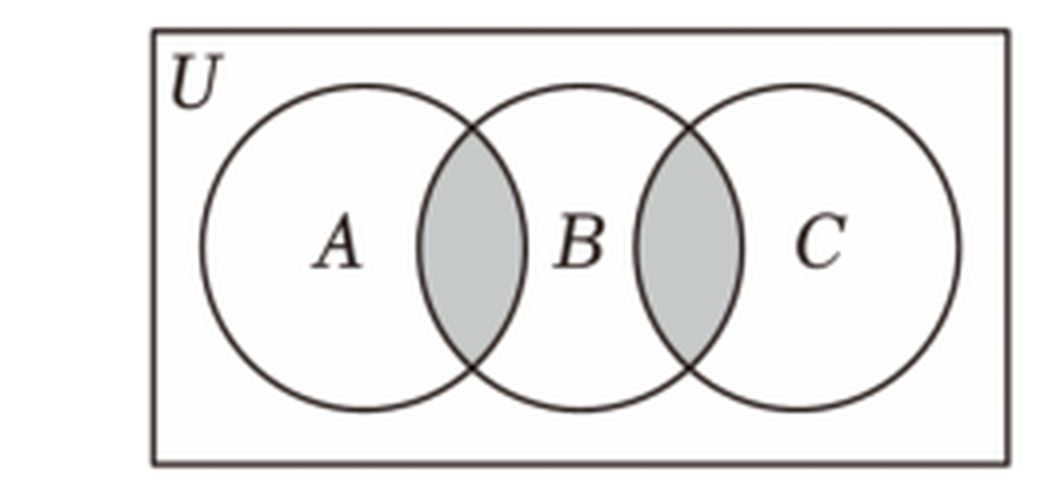
\includegraphics[width=0.30\textwidth]{figures/venn_ABC_lenses.png}
\end{center}

\keepwithprev
A. $B\cap(A\cup C)$\qquad\qquad\qquad B. $B\cap(A\cap C)$

C. $B\cap\complement_U(A\cup C)$\qquad\qquad D. $(A\cup B)\cap(B\cup C)$

\ans{$A$}

\ifanswer
\solbegin
\step{由图中阴影部分得，阴影为集合 $A$、$B$ 的交集和 $B$、$C$ 的交集的并集，}
\step{故阴影部分可表示为 $(A\cap B)\cup(B\cap C)$ 或 $B\cap(A\cup C)$，
故 $A$ 正确. 故选 $A$.}
\solend

\fi

\item 设集合 $P_1=\{x\mid x^2+ax+1>0\}$，$P_2=\{x\mid x^2+ax+2>0\}$，
$Q_1=\{x\mid x^2+x+b>0\}$，$Q_2=\{x\mid x^2+2x+b>0\}$，其中 $a$、$b\in\R$，
对于下列两个命题：①存在 $a$，$P_1$ 不是 $P_2$ 的子集；②存在 $b$ 使得 $Q_1$ 是 $Q_2$
的子集. 下列说法正确的是\mbox{（\quad）}

\keepwithprev
A. ①是真命题，②是假命题\qquad B. ①是假命题，②是真命题

C. ①②都是真命题\qquad\qquad\quad D. ①②都是假命题

\ans{$B$}

\ifanswer
\solbegin
\step{对于集合 $P_1=\{x\mid x^2+ax+1>0\}$，$P_2=\{x\mid x^2+ax+2>0\}$，}
\step{得当 $m\in P_1$ 时，即 $m^2+am+1>0$，得 $m^2+am+2>0$，}
\step{即有 $m\in P_2$，得对任意 $a$，$P_1$ 是 $P_2$ 的子集，故①错误；}
\step{对于集合 $Q_1=\{x\mid x^2+x+b>0\}$，$Q_2=\{x\mid x^2+2x+b>0\}$，}
\step{当 $b=6$ 时，$Q_1=\{x\mid x^2+x+6>0\}=\R$，$Q_2=\{x\mid x^2+2x+6>0\}=\R$，}
\step{得 $Q_1$ 是 $Q_2$ 的子集，所以存在 $b$，使得 $Q_1$ 是 $Q_2$ 的子集，故②正确；}
\step{故选 $B$.}
\solend

\fi

\item 设 $a$、$b\in\R$，则“$a+b>2$ 且 $ab>1$”是“$a>1$ 且 $b>1$”的\mbox{（\quad）}

\keepwithprev
A. 充要条件\qquad\qquad\qquad B. 充分不必要条件

C. 必要不充分条件\qquad\quad D. 既不充分又不必要条件

\ans{$C$}

\ifanswer
\solbegin
\step{因为 $a>1$ 且 $b>1$，所以 $a+b>2$ 且 $ab>1$，}
\step{若已知 $a+b>2$ 且 $ab>1$，可取 $a=\dfrac12$，$b=8$，也满足已知，}
\step{所以“$a+b>2$ 且 $ab>1$”是“$a>1$ 且 $b>1$”的必要不充分条件，故选 $C$.}
\solend

\fi

\item 十七世纪，数学家费马提出猜想：“对任意正整数 $n>2$，关于 $x$、$y$、$z$ 的方程
$x^n+y^n=z^n$ 没有正整数解”. 1995 年数学家安德鲁·怀尔斯发表了完成的证明过程，使它
终成费马大定理. 对费马大定理，若用反证法证明，第一步是假设猜想不成立，即\mbox{（\quad）}

\keepwithprev
A. 对任意正整数 $n>2$，关于 $x$、$y$、$z$ 的方程 $x^n+y^n=z^n$ 都有正整数解

B. 对任意正整数 $n>2$，关于 $x$、$y$、$z$ 的方程 $x^n+y^n=z^n$ 至少存在一组正整数解

C. 存在正整数 $n\leqslant2$，关于 $x$、$y$、$z$ 的方程 $x^n+y^n=z^n$ 至少存在一组正整数解

D. 存在正整数 $n>2$，关于 $x$、$y$、$z$ 的方程 $x^n+y^n=z^n$ 至少存在一组正整数解

\ans{$D$}

\end{enumerate}

\bigsec{三、解答题}

\begin{enumerate}
\setcounter{enumi}{16}

\item 已知 $a$、$b$、$c$ 都是实数，且 $a+b+c=0$，$abc=1$，求证：$a$、$b$、$c$ 中必有一个
大于 $\dfrac32$.

\ifanswer
\solbegin
\step{由 $a+b+c=0$，$abc=1$，得 $a$、$b$、$c$ 中一个正数，两个负数，}
\step{不妨设 $c>0$，由题意得 $a+b=-c,ab=\dfrac1c$，}
\step{由根与系数的关系得 $a$、$b$ 是关于 $x$ 的方程 $x^2+cx+\dfrac1c=0$ 的两个根，}
\step{则 $\Delta=c^2-\dfrac4c=\dfrac{c^3-4}{c}\geqslant0$，}
\step{因为 $c>0$，所以 $c^3\geqslant4$，得 $c\geqslant\sqrt[3]{4}$，}
\step{又 $\dfrac32=\sqrt[3]{\left(\dfrac32\right)^3}=\sqrt[3]{\dfrac{27}{8}}<\sqrt[3]{4}$，}
\step{所以 $c>\dfrac32$，即 $a$、$b$、$c$ 中必有一个大于 $\dfrac32$.}
\solend

\fi

\ansspace[6]

\item 已知关于 $x$ 的一元二次方程 $x^2-mx+4m^2-3=0$ 的两个实根分别为 $x_1,x_2$.

\begin{enumerate}[label=(\arabic*)]
\item $x_1,x_2$ 均为正根，求实数 $m$ 的取值范围；
\item 若 $x_1,x_2$ 满足：$x_1+x_2=x_1x_2$，求实数 $m$ 的值.
\end{enumerate}

\ifanswer
\solbegin
\stepm{(1)}{由 $x_1,x_2$ 均为正根，得}
\step{$\begin{cases}\Delta=(-m)^2-4(4m^2-3)\geqslant0\\ x_1+x_2=m>0\\ x_1\cdot x_2=4m^2-3>0\end{cases}$，}
\step{解得 $\begin{cases}-\dfrac{2\sqrt5}{5}\leqslant m\leqslant\dfrac{2\sqrt5}{5}\\[4pt]
m>0\\[4pt] m\leqslant-\dfrac{\sqrt3}{2}$ 或 $m\geqslant\dfrac{\sqrt3}{2}\end{cases}$，}
\step{即 $\dfrac{\sqrt3}{2}\leqslant m\leqslant\dfrac{2\sqrt5}{5}$；}
\stepm{(2)}{由 (1) 得
$\begin{cases}-\dfrac{2\sqrt5}{5}\leqslant m\leqslant\dfrac{2\sqrt5}{5}\\[4pt]
m=4m^2-3\end{cases}$，解得 $m=1$（舍去）或 $m=-\dfrac34$，}
\step{则 $m=-\dfrac34$.}
\solend

\fi

\ansspace[6]

\item 已知集合 $A=\{x\mid m-1<x<m^2+1\}$，$B=\{x\mid-2<x<2\}$.

\begin{enumerate}[label=(\arabic*)]
\item 当 $m=2$ 时，求 $A\cup B$、$A\cap B$、$\complement_R B$、$A\cap(\complement_R B)$；
\item 若“$x\in A$”是“$x\in B$”成立的必要不充分条件，求实数 $m$ 的取值范围.
\end{enumerate}

\ifanswer
\solbegin
\stepm{(1)}{$m=2$ 时，$A=\{x\mid1<x<5\}$，且 $B=\{x\mid-2<x<2\}$，}
\step{所以 $A\cup B=\{x\mid-2<x<5\}$，$A\cap B=\{x\mid1<x<2\}$，}
\step{$\complement_R B=\{x\mid x\leqslant-2$ 或 $x\geqslant2\}$，
$A\cap(\complement_R B)=\{x\mid2\leqslant x<5\}$；}
\stepm{(2)}{若“$x\in A$”是“$x\in B$”成立的必要不充分条件，则 $B\subset A$，}
\step{所以 $\begin{cases}m-1<-2\\ m^2+1\geqslant2\end{cases}$
或 $\begin{cases}m-1\leqslant-2\\ m^2+1>2\end{cases}$，解得 $m<-1$，}
\step{故 $m$ 的取值范围为 $(-\infty,-1)$.}
\solend

\fi

\ansspace[6]

\item 已知 $m\in\R$，集合 $A=\{x\mid|x-1|\leqslant2\}$，集合
$B=\{x\mid m-3<x\leqslant m+2\}$.

\begin{enumerate}[label=(\arabic*)]
\item 若“$x\in A$”是“$x\in B$”的充分不必要条件，求 $m$ 的取值范围；
\item 若命题“$\forall x\in B$，$x\in\complement_R A$”是真命题，求 $m$ 的取值范围；
\item 若命题“$\exists x\in A$，$x\in B$”是真命题，求 $m$ 的取值范围.
\end{enumerate}

\ifanswer
\solbegin
\stepm{(1)}{集合 $A=\{x\mid|x-1|\leqslant2\}=\{x\mid-1\leqslant x\leqslant3\}$，}
\step{若“$x\in A$”是“$x\in B$”的充分不必要条件，则 $A\subset B$，}
\step{所以 $\begin{cases}m-3<-1\\ 3\leqslant m+2\end{cases}$，解得 $1\leqslant m<2$，}
\step{当 $m=1$ 时，$B=\{x\mid-2<x\leqslant3\}$，符合题意，}
\step{所以 $m$ 的取值范围是 $\{m\mid1\leqslant m<2\}$.}
\stepm{(2)}{若命题“$\forall x\in B$，$x\in\complement_R A$”是真命题，则 $B\subset\complement_R A$，}
\step{又 $\complement_R A=\{x\mid x<-1$ 或 $x>3\}$，$B\neq\varnothing$，
所以 $m+2<-1$ 或 $m-3\geqslant3$，}
\step{解得 $m<-3$ 或 $m\geqslant6$，所以 $\{m\mid m<-3$ 或 $m\geqslant6\}$；}
\stepm{(3)}{因为 $\exists x\in A$，$x\in B$ 是真命题，所以 $A\cap B\neq\varnothing$，}
\step{当 $A\cap B=\varnothing$ 时，所以 $m+2<-1$ 或 $m-3\geqslant3$，
即 $m<-3$ 或 $m\geqslant6$，}
\step{所以当 $A\cap B\neq\varnothing$ 时，$m$ 的取值范围是 $\{m\mid-3\leqslant m<6\}$，}
\step{则 $m$ 的取值范围是 $\{m\mid-3\leqslant m<6\}$.}
\solend

\fi

\ansspace[6]

\item 对于函数 $f(x)$，若 $f(x_0)=x_0$，则称 $x_0$ 为 $f(x)$ 的“不动点”；若
$f[f(x_0)]=x_0$，则称 $x_0$ 为 $f(x)$ 的“稳定点”. 函数 $f(x)$ 的“不动点”和“稳定点”
的集合分别记为 $A$ 和 $B$，即 $A=\{x\mid f(x)=x\}$，$B=\{x\mid f[f(x)]=x\}$.

\begin{enumerate}[label=(\arabic*)]
\item 设函数 $f(x)=3x+4$，求集合 $A$ 和 $B$；
\item 求证：$A\sub B$；
\item 设函数 $f(x)=ax^2+bx+c(a\neq0)$，且 $A=\varnothing$，求证：$B=\varnothing$.
\end{enumerate}

\ifanswer
\solbegin
\stepm{(1)}{令 $f(x)=3x+4=x$，解得 $x=-2$，故有 $A=\{-2\}$，}
\step{由于 $f[f(x)]=3(3x+4)+4=9x+16$，}
\step{令 $9x+16=x$，得 $x=-2$，故有 $B=\{-2\}$；}
\stepm{(2)}{若 $A=\varnothing$，则 $A\sub B$ 显然成立；}
\step{若 $A\neq\varnothing$，设 $t\in A$，则 $f(t)=t$，$f(f(t))=f(t)=t$，}
\step{所以 $t\in B$，故 $A\sub B$.}
\stepm{(3)}{因为 $A=\{x\mid f(x)=x\}=\varnothing$，所以 $ax^2+bx+c=x$ 无解，}
\step{即 $\Delta=(b-1)^2-4a<0$，}
\step{①当 $a>0$ 时，二次函数 $y=f(x)-x$，}
\step{即 $y=ax^2+(b-1)x+c$ 的图象在 $x$ 轴的上方，}
\step{所以 $\forall x\in\R$，$f(x)-x>0$ 恒成立，所以 $\forall x\in\R$，
$f(x)>x$ 恒成立，}
\step{所以 $\forall x\in\R$，$f[f(x)]>f(x)>x$ 恒成立，即 $B=\varnothing$；}
\step{②当 $a<0$ 时，同理可证 $B=\varnothing$；}
\step{综上，对于函数 $f(x)=ax^2+bx+c(a\neq0)$，当 $A=\varnothing$ 时，$B=\varnothing$.}
\solend

\fi

\ansspace*[10]

\end{enumerate}

\end{document}
"
%
% 原始材料是微信公众号图文（公众号「魔都数学加油站」连载「27学年高一 26」，2026-09-21 发布，
% 原文标题「27学年高一26——2026-2027年上海市交附闵行高一上周练2」），
% 正文为 10 张 PNG 页（1080×1527，各页同尺寸）。原文本身就是一份**讲评版**——
% 题目下方直接印出【解析】（本卷无单独的【答案】行，填空题答案都写在解析里）。
% 试题文字与解析均照原卷录入，未改内容。卷面的粉色斜水印「魔都数学加油站」属水印，未录入。
%
% 卷首标题：原卷印作「2026-2027 年交附闵行高一上周练 2」（公众号标题里的「上海市」
% 三字卷面标题行没有，本稿照卷面），年份区间按全稿惯例排 en dash，前缀照原卷保留「年」。
%
% 与原卷的排版差异（均已在 README「说明」中交代）：
%   ① 原文自**第 3 题**起（第 1、2 题未在该文中发布），故本稿题号亦自 3 起；
%   ② 原卷本就印有「一、填空题」「二、选择题」「三、解答题」三节标题，本稿照原卷分节，
%      只把标题改排成全稿统一的「大节标题」样式；
%   ③ 原卷第 16 题的答案「D」直接印在题干末尾的括号内（原卷把括号连同 D 单独占一行），
%      第 13—15 题的括号空着、答案写在解析末句「故选 A／B／C」里；填空题的答案也都嵌在
%      解析里，本稿统一改为试卷版隐去、答案版以 \ans{} 给出（选择题另附【解析】）；
%   ④ 子集符号原卷两种并用：第 4 题题干与第 8 题、第 21(2) 题等作带下划线的 $\subseteq$，
%      第 19(2)、20(1)(2) 题作真包含的 $\subset$，本稿分别照录为 $\sub$ 与 $\subset$；
%   ⑤ 补集符号原卷作 $\complement_R$、$\complement_U$（第 4 题命题④、第 13 题选项 C、
%      第 19—20 题），本稿照录；
%   ⑥ 原卷的实数集 R 一律作斜体（第 11 题「$a\in R$」、第 14 题「$a$、$b\in R$」与解析的
%      $\{x\mid x^2+x+6>0\}=R$ 等），本稿按全稿惯例统一写作 $\R$；
%   ⑦ 原卷填空的横线约两个字宽，本稿按全稿惯例统一排 \blankline[4.4em]；
%   ⑧ 原卷未印副标题，本稿按全稿惯例补出副标题「集合与常用逻辑用语」；
%   ⑨ 第 13 题的 Venn 图原卷印在题干右侧（第 5 页），本稿移至题干之后；
%      图取原卷截图、4× LANCZOS 放大（figures/venn_ABC_lenses.png，
%      阴影为 $A\cap B$ 与 $B\cap C$ 两个交带，即 $(A\cap B)\cup(B\cap C)$）。
%
% 原卷存疑一处（照抄原卷、未改，见源码中该处上方注释）：
%   ① 第 12 题【解析】首步的方程组里印 $t<2$，而其后三处与末行答案都作 $t\leqslant2$
%      （$\left[\dfrac85,\dfrac{17}{10}\right)\cup\left(\dfrac95,2\right]$ 含 $2$）——
%      按题意 $N=\left\{x\mid t-\dfrac35\leqslant x\leqslant t\right\}\sub\{x\mid1\leqslant x\leqslant2\}$
%      只要求 $t\leqslant2$（$t=2$ 时 $N=\left[\dfrac75,2\right]$ 确实含于其中），
%      故方程组里的 $t<2$ 应是原卷笔误；本稿两处都照原卷录入、未互相迁就。
% 另：第 20(3) 题解析末两行原卷即作同话重复，照原卷录入。

\documentclass[a4paper,11pt]{article}
\usepackage{common}

\begin{document}

\examtitlest[3]{2026--2027 年交附闵行高一上周练 2}{集合与常用逻辑用语}

\bigsec{一、填空题}

\begin{enumerate}
\setcounter{enumi}{2}

\item 命题甲：集合 $M=\{x\mid kx^2-2kx+1=0\}$ 为空集；命题乙：关于 $x$ 的不等式
$x^2+(k-1)x+4>0$ 的解集为 $\R$. 若命题甲、乙中有且只有一个是真命题，则实数 $k$ 的取
值范围是 \blankline[4.4em].

\ifanswer
\solbegin
\step{因为集合 $M=\{x\mid kx^2-2kx+1=0\}$ 为空集，}
\step{当 $k\neq0$ 时，$\Delta=(-2k)^2-4k<0$，解得 $0<k<1$，}
\step{当 $k=0$ 时，方程变为 $1=0$，无解，满足题意，故 $0\leqslant k<1$；}
\step{又关于 $x$ 的不等式 $x^2+(k-1)x+4>0$ 的解集为 $\R$，}
\step{所以 $\Delta'=(k-1)^2-4\times4<0$，解得 $-3<k<5$，}
\step{当甲命题为真，乙命题为假时，无解，}
\step{当甲命题为假，乙命题为真时，$k\in(-3,0)\cup[1,5)$.}
\solend

\fi

\item 对任意 $A$、$B\sub\R$，记 $A\oplus B=\{x\mid x\in A\cup B,x\notin A\cap B\}$，
并称 $A\oplus B$ 为集合 $A$、$B$ 的对称差. 例如：若 $A=\{1,2,3\},B=\{2,3,4\}$，
则 $A\oplus B=\{1,4\}$. 下列命题中，为真命题的是 \blankline[4.4em].

\keepwithprev
①若 $A$、$B\sub\R$ 且 $A\oplus B\sub A$，则 $A\sub B$

②若 $A$、$B\sub\R$ 且 $A\oplus B=\varnothing$，则 $A=B$

③若 $A$、$B\sub\R$ 且 $A\oplus B=B$，则 $A=\varnothing$

④对任意 $A$、$B\sub\R$，都有 $A\oplus B=\complement_R A\oplus\complement_R B$

\ans{②③④}

\ifanswer
\solbegin
\step{对于①，因为 $A\oplus B\sub A$，
所以 $\{x\mid x\in A\cup B,x\notin A\cap B\}\sub A$，}
\step{故 $B\sub A$，①错误；}
\step{对于②，$A$、$B\sub\R$ 且 $A\oplus B=\varnothing$，
则 $\varnothing=\{x\mid x\in A\cup B,x\notin A\cap B\}$，}
\step{即 $A\cup B=A\cap B$，所以 $A=B$，②正确；}
\step{对于③，$A$、$B\sub\R$ 且 $A\oplus B=B$，
则 $B=\{x\mid x\in A\cup B,x\notin A\cap B\}$，}
\step{故 $A\sub B$，且 $B$ 中元素不在 $A\cap B$ 中，故 $A=\varnothing$，③正确；}
\step{对于④，$\complement_R A\oplus\complement_R B
=\{x\mid x\in\complement_R A\cup\complement_R B,x\notin\complement_R A\cap\complement_R B\}$，}
\step{其中 $\complement_R A\cup\complement_R B=\complement_R(A\cap B)$，
$\complement_R A\cap\complement_R B=\complement_R(A\cup B)$，}
\step{故 $\complement_R A\oplus\complement_R B
=\{x\mid x\in\complement_R(A\cap B),x\notin\complement_R(A\cup B)\}
=\{x\mid x\in A\cup B,x\notin A\cap B\}$，}
\step{而 $A\oplus B=\{x\mid x\in A\cup B,x\notin A\cap B\}$，
故 $A\oplus B=\complement_R A\oplus\complement_R B$，④正确.}
\step{故正确的是②③④.}
\solend

\fi

\item 已知 $A=\{a_1,a_2,a_3,a_4\},B=\{a^2\mid a\in A\}$，其中 $a_1<a_2<a_3<a_4$，
且 $a_1$、$a_2$、$a_3$、$a_4$ 均为整数，若 $A\cap B=\{a_3,a_4\},a_1+a_3=0$，
且 $A\cup B$ 中的所有元素之和为 $270$，则集合 $A$ 中所有元素之和为 \blankline[4.4em].

\ifanswer
\solbegin
\step{$A=\{a_1,a_2,a_3,a_4\},B=\{a^2\mid a\in A\}$，
因为 $A\cap B=\{a_3,a_4\},a_1+a_3=0$，}
\step{所以 $A=\{a_1,a_2,a_3,a_4\},B=\left\{a_1^2,a_2^2,a_4^2\right\}$，}
\step{若 $a_1^2=a_3$，则 $a_1=-1,a_3=1$，则 $a_2=0$，
此时 $A=\{-1,0,1,a_4\},B=\{0,1,a_4^2\}$，}
\step{因为 $A\cup B$ 中的所有元素之和为 $270$，
所以 $-1+0+1+a_4+1+a_4^2=270$，}
\step{无正整数解，舍去；}
\step{若 $a_2^2=a_3$，① $a_4^2=a_4$，所以 $a_4=1$，矛盾；}
\step{② $a_1^2=a_4$，此时 $A\cup B=\left\{-a_2^2,a_2,a_2^2,a_1^2,a_4^2\right\}$，
所以 $a_2^8+a_2^4+a_2=270$，}
\step{所以 $a_2=-2$，此时 $a_1=-4,a_2=-2,a_3=4,a_4=16$；}
\step{若 $a_4^2=a_3$，显然不成立；}
\step{综上，集合 $A$ 中所有元素之和为 $-4-2+4+16=14$.}
\solend

\fi

\item 将集合 $M=\{a_1,a_2,a_3,\cdots,a_n\}$ 分拆成两个集合 $A_i$ 和 $B_j$，且
$M\supseteq A_i\cup B_j$，$A_i\cap B_j=\varnothing$，这样的分拆方法共有 \blankline[4.4em] 种.

\ifanswer
\solbegin
\step{按集合 $A_i$ 中的元素个数进行分类：}
\step{若 $A_i$ 中有 $0$ 个元素（即 $C_n^0$ 种）时，则 $B_j$ 有 $2^n$ 种，
共有 $2^nC_n^0$ 种；}
\step{若 $A_i$ 中有 $1$ 个元素（即 $C_n^1$ 种）时，则 $B_j$ 有 $2^{n-1}$ 种，
共有 $2^{n-1}C_n^1$ 种；}
\step{若 $A_i$ 中有 $2$ 个元素（即 $C_n^2$ 种）时，则 $B_j$ 有 $2^{n-2}$ 种，
共有 $2^{n-2}C_n^2$ 种；}
\step{若 $A_i$ 中有 $3$ 个元素（即 $C_n^3$ 种）时，则 $B_j$ 有 $2^{n-3}$ 种，
共有 $2^{n-3}C_n^3$ 种；}
\step{若 $A_i$ 中有 $n$ 个元素（即 $C_n^n$ 种）时，则 $B_j$ 有 $2^0$ 种，
共有 $2^0C_n^n$ 种；}
\step{得 $2^nC_n^0+2^{n-1}C_n^1+2^{n-2}C_n^2+\cdots+2^0C_n^n=(1+2)^n$，
故这样的分拆方法有 $3^n$ 种.}
\solend

\fi

\item 已知集合 $A=\{x\mid x<2,x\in\Z\}$，$B=\{x\mid x>0,x\in\Z\}$，则
$A\cap B=$ \blankline[4.4em].

\ifanswer
\solbegin
\step{因为 $A=\{x\mid x<2,x\in\Z\}$，$B=\{x\mid x>0,x\in\Z\}$，}
\step{所以 $A\cap B=\{x\mid0<x<2,x\in\Z\}=\{1\}$.}
\solend

\fi

\item 已知集合 $A=\{x\mid(a-1)x^2+3x-2=0\}$，$B=\{x\mid x^2-3x+2=0\}$，若
$A\sub B$，求实数 $a$ 的取值范围是 \blankline[4.4em].

\ifanswer
\solbegin
\step{由方程 $x^2-3x+2=0$，解得 $x=1$ 或 $x=2$，即 $B=\{1,2\}$，}
\step{因为 $A\sub B$，所以 $A=\varnothing$ 或 $A=\{1\}$ 或 $A=\{2\}$ 或 $A=\{1,2\}$，}
\step{当 $A=\varnothing$ 时，
则 $\begin{cases}a\neq1\\ \Delta=3^2-4(a-1)\times(-2)<0\end{cases}$，
解得 $a<-\dfrac18$；}
\step{将 $x=1$ 代入方程 $(a-1)x^2+3x-2=0$，得 $a=0$，}
\step{此时 $A=\{x\mid-x^2+3x-2=0\}=\{1,2\}$，满足条件；}
\step{将 $x=2$ 代入方程 $(a-1)x^2+3x-2=0$，得到 $a=0$，上面已经验证满足条件；}
\step{综上所述，$a$ 的取值范围是 $\left(-\infty,-\dfrac18\right)\cup\{0\}$.}
\solend

\fi

\item 已知方程 $x^2-3x+a=0$ 的两根都大于 $1$，则 $a$ 的取值范围为 \blankline[4.4em].

\ifanswer
\solbegin
\step{由题意得 $\Delta=9-4a\geqslant0$，$x_1+x_2=3$，$x_1x_2=a$，
所以 $a\leqslant\dfrac94$，}
\step{则 $(x_1-1)(x_2-1)=x_1x_2-(x_1+x_2)+1=a-3+1>0$，所以 $a>2$，}
\step{故 $a$ 的范围为 $\left(2,\dfrac94\right]$.}
\solend

\fi

\item 设 $x_1$、$x_2$ 是方程 $x^2+x-3=0$ 的两个实数根，则 $x_1^2-x_2+2024=$
\blankline[4.4em].

\ifanswer
\solbegin
\step{由题意得 $x_1^2=3-x_1$，$x_1+x_2=-1$，}
\step{则 $x_1^2-x_2+2024=3-x_1-x_2+2024=2027-(-1)=2028$.}
\solend

\fi

\item 已知 $a\in\R$，若关于 $x$ 的方程 $x^2+ax+a^2-8=0$ 有两个实根 $x_1$、$x_2$，且
$\dfrac1{x_1}+\dfrac1{x_2}=-\dfrac12$，则 $a$ 的值为 \blankline[4.4em].

\ifanswer
\solbegin
\step{由题意得 $\Delta=a^2-4(a^2-8)=32-3a^2\geqslant0$，
解得 $a^2\leqslant\dfrac{32}{3}$，}
\step{由韦达定理得 $x_1+x_2=-a$，$x_1x_2=a^2-8$，}
\step{则 $\dfrac1{x_1}+\dfrac1{x_2}=\dfrac{x_1+x_2}{x_1x_2}
=\dfrac{-a}{a^2-8}=-\dfrac12$，}
\step{即 $a^2-2a-8=(a-4)(a+2)=0$，解得 $a=4$ 或 $a=-2$.}
\step{又 $a^2\leqslant\dfrac{32}{3}$，则 $a=-2$.}
\solend

\fi

\item 定义集合 $P=\{x\mid a\leqslant x\leqslant b\}$ 的“长度”是 $b-a$，其中 $a$、
$b\in\R$. 已知集合 $M=\left\{x\mid\dfrac65\leqslant x\leqslant\dfrac{17}{10}\right\}$，
$N=\left\{x\mid t-\dfrac35\leqslant x\leqslant t\right\}$，且 $M$、$N$ 都是集合
$\{x\mid1\leqslant x\leqslant2\}$ 的子集，若集合 $M\cup N$ 的“长度”大于 $\dfrac35$，
则 $t$ 的取值范围是 \blankline[4.4em].

\ifanswer
\solbegin
\step{因为 $N=\left\{x\mid t-\dfrac35\leqslant x\leqslant t\right\}$
是集合 $\{x\mid1\leqslant x\leqslant2\}$ 的子集，}
% 注：下一行方程组里的 $t<2$ 系原卷所印（本稿照录），与其后三处及末行答案的
%     $t\leqslant2$ 自相矛盾——按题意应为 $t\leqslant2$，见文件头「原卷存疑」①。
\step{所以 $\begin{cases}t-\dfrac35\geqslant1\\[2pt] t<2\end{cases}$，
解得 $\dfrac85\leqslant t\leqslant2$，}
\step{又 $M=\left\{x\mid\dfrac65\leqslant x\leqslant\dfrac{17}{10}\right\}$，
得集合 $M$ 的“长度”为 $\dfrac{17}{10}-\dfrac65=\dfrac12$，}
\step{又 $N=\left\{x\mid t-\dfrac35\leqslant x\leqslant t\right\}$，
要使集合 $M\cup N$ 的“长度”大于 $\dfrac35$，}
\step{若 $M\cup N=\left\{x\mid t-\dfrac35\leqslant x\leqslant\dfrac{17}{10}\right\}$，
则 $\dfrac{17}{10}-t+\dfrac35>\dfrac35$，所以 $t<\dfrac{17}{10}$，}
\step{又 $\dfrac85\leqslant t\leqslant2$，所以 $\dfrac85\leqslant t<\dfrac{17}{10}$；}
\step{若 $M\cup N=\left\{x\mid\dfrac65\leqslant x\leqslant t\right\}$，
则 $t-\dfrac65>\dfrac35$，所以 $t>\dfrac95$，}
\step{又 $\dfrac85\leqslant t\leqslant2$，所以 $\dfrac95<t\leqslant2$；}
\step{则 $t$ 的取值范围是 $\left[\dfrac85,\dfrac{17}{10}\right)\cup\left(\dfrac95,2\right]$.}
\solend

\fi

\end{enumerate}

% 第 13 题是「题干 + 图 + 选项」约 5.7cm 的一整块（图 0.30\textwidth、宽高比 0.477 → 高 2.29cm，
% 加题干 1 行、选项 2 行与段间距）。`\keepwithprev` 只挡得住「题干—选项」之间，挡不住
% 夹在中间的图——实测断点落在题干之后，题干孤零零留在 p1、图与四个选项整页翻到 p2
% （切页审计的 A 类）。故照 高一30 第 4 题的成例先量一次页高；**守卫要放在 `\bigsec` 之前**
% 连节标题一起量（放标题之后会把「二、选择题」孤立在页末，正是 高一40 修过的那类 B 类）。
% 7cm ＝ 节标题约 1.1cm ＋ 第 13 题那块约 5.7cm（留少量余量）。
\needvspace{7cm}
\bigsec{二、选择题}

\begin{enumerate}
\setcounter{enumi}{12}

\item 图中阴影部分用集合符号可以表示为\mbox{（\quad）}

\begin{center}
% 图取原卷截图、4× LANCZOS 放大（原卷把图印在题干右侧，本稿移至此处，见文件头⑨）。
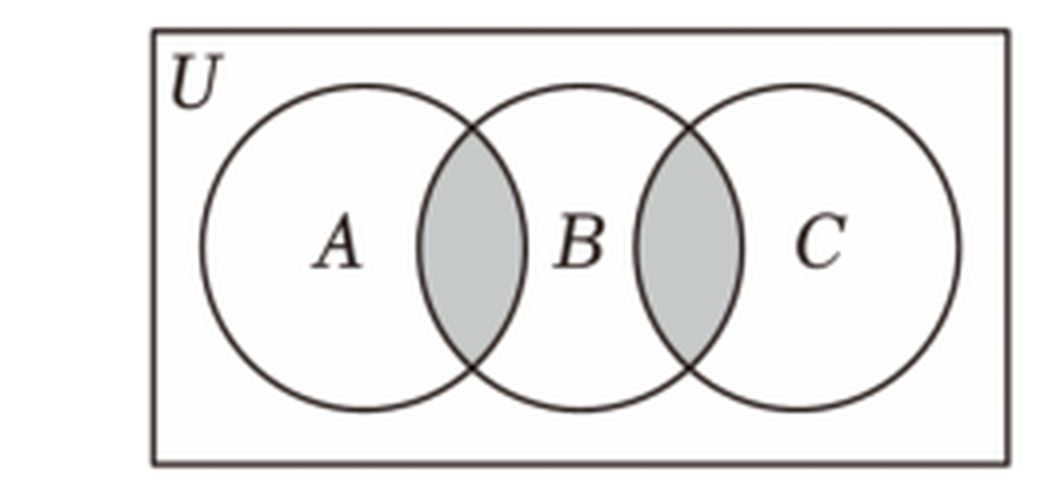
\includegraphics[width=0.30\textwidth]{figures/venn_ABC_lenses.png}
\end{center}

\keepwithprev
A. $B\cap(A\cup C)$\qquad\qquad\qquad B. $B\cap(A\cap C)$

C. $B\cap\complement_U(A\cup C)$\qquad\qquad D. $(A\cup B)\cap(B\cup C)$

\ans{$A$}

\ifanswer
\solbegin
\step{由图中阴影部分得，阴影为集合 $A$、$B$ 的交集和 $B$、$C$ 的交集的并集，}
\step{故阴影部分可表示为 $(A\cap B)\cup(B\cap C)$ 或 $B\cap(A\cup C)$，
故 $A$ 正确. 故选 $A$.}
\solend

\fi

\item 设集合 $P_1=\{x\mid x^2+ax+1>0\}$，$P_2=\{x\mid x^2+ax+2>0\}$，
$Q_1=\{x\mid x^2+x+b>0\}$，$Q_2=\{x\mid x^2+2x+b>0\}$，其中 $a$、$b\in\R$，
对于下列两个命题：①存在 $a$，$P_1$ 不是 $P_2$ 的子集；②存在 $b$ 使得 $Q_1$ 是 $Q_2$
的子集. 下列说法正确的是\mbox{（\quad）}

\keepwithprev
A. ①是真命题，②是假命题\qquad B. ①是假命题，②是真命题

C. ①②都是真命题\qquad\qquad\quad D. ①②都是假命题

\ans{$B$}

\ifanswer
\solbegin
\step{对于集合 $P_1=\{x\mid x^2+ax+1>0\}$，$P_2=\{x\mid x^2+ax+2>0\}$，}
\step{得当 $m\in P_1$ 时，即 $m^2+am+1>0$，得 $m^2+am+2>0$，}
\step{即有 $m\in P_2$，得对任意 $a$，$P_1$ 是 $P_2$ 的子集，故①错误；}
\step{对于集合 $Q_1=\{x\mid x^2+x+b>0\}$，$Q_2=\{x\mid x^2+2x+b>0\}$，}
\step{当 $b=6$ 时，$Q_1=\{x\mid x^2+x+6>0\}=\R$，$Q_2=\{x\mid x^2+2x+6>0\}=\R$，}
\step{得 $Q_1$ 是 $Q_2$ 的子集，所以存在 $b$，使得 $Q_1$ 是 $Q_2$ 的子集，故②正确；}
\step{故选 $B$.}
\solend

\fi

\item 设 $a$、$b\in\R$，则“$a+b>2$ 且 $ab>1$”是“$a>1$ 且 $b>1$”的\mbox{（\quad）}

\keepwithprev
A. 充要条件\qquad\qquad\qquad B. 充分不必要条件

C. 必要不充分条件\qquad\quad D. 既不充分又不必要条件

\ans{$C$}

\ifanswer
\solbegin
\step{因为 $a>1$ 且 $b>1$，所以 $a+b>2$ 且 $ab>1$，}
\step{若已知 $a+b>2$ 且 $ab>1$，可取 $a=\dfrac12$，$b=8$，也满足已知，}
\step{所以“$a+b>2$ 且 $ab>1$”是“$a>1$ 且 $b>1$”的必要不充分条件，故选 $C$.}
\solend

\fi

\item 十七世纪，数学家费马提出猜想：“对任意正整数 $n>2$，关于 $x$、$y$、$z$ 的方程
$x^n+y^n=z^n$ 没有正整数解”. 1995 年数学家安德鲁·怀尔斯发表了完成的证明过程，使它
终成费马大定理. 对费马大定理，若用反证法证明，第一步是假设猜想不成立，即\mbox{（\quad）}

\keepwithprev
A. 对任意正整数 $n>2$，关于 $x$、$y$、$z$ 的方程 $x^n+y^n=z^n$ 都有正整数解

B. 对任意正整数 $n>2$，关于 $x$、$y$、$z$ 的方程 $x^n+y^n=z^n$ 至少存在一组正整数解

C. 存在正整数 $n\leqslant2$，关于 $x$、$y$、$z$ 的方程 $x^n+y^n=z^n$ 至少存在一组正整数解

D. 存在正整数 $n>2$，关于 $x$、$y$、$z$ 的方程 $x^n+y^n=z^n$ 至少存在一组正整数解

\ans{$D$}

\end{enumerate}

\bigsec{三、解答题}

\begin{enumerate}
\setcounter{enumi}{16}

\item 已知 $a$、$b$、$c$ 都是实数，且 $a+b+c=0$，$abc=1$，求证：$a$、$b$、$c$ 中必有一个
大于 $\dfrac32$.

\ifanswer
\solbegin
\step{由 $a+b+c=0$，$abc=1$，得 $a$、$b$、$c$ 中一个正数，两个负数，}
\step{不妨设 $c>0$，由题意得 $a+b=-c,ab=\dfrac1c$，}
\step{由根与系数的关系得 $a$、$b$ 是关于 $x$ 的方程 $x^2+cx+\dfrac1c=0$ 的两个根，}
\step{则 $\Delta=c^2-\dfrac4c=\dfrac{c^3-4}{c}\geqslant0$，}
\step{因为 $c>0$，所以 $c^3\geqslant4$，得 $c\geqslant\sqrt[3]{4}$，}
\step{又 $\dfrac32=\sqrt[3]{\left(\dfrac32\right)^3}=\sqrt[3]{\dfrac{27}{8}}<\sqrt[3]{4}$，}
\step{所以 $c>\dfrac32$，即 $a$、$b$、$c$ 中必有一个大于 $\dfrac32$.}
\solend

\fi

\ansspace[6]

\item 已知关于 $x$ 的一元二次方程 $x^2-mx+4m^2-3=0$ 的两个实根分别为 $x_1,x_2$.

\begin{enumerate}[label=(\arabic*)]
\item $x_1,x_2$ 均为正根，求实数 $m$ 的取值范围；
\item 若 $x_1,x_2$ 满足：$x_1+x_2=x_1x_2$，求实数 $m$ 的值.
\end{enumerate}

\ifanswer
\solbegin
\stepm{(1)}{由 $x_1,x_2$ 均为正根，得}
\step{$\begin{cases}\Delta=(-m)^2-4(4m^2-3)\geqslant0\\ x_1+x_2=m>0\\ x_1\cdot x_2=4m^2-3>0\end{cases}$，}
\step{解得 $\begin{cases}-\dfrac{2\sqrt5}{5}\leqslant m\leqslant\dfrac{2\sqrt5}{5}\\[4pt]
m>0\\[4pt] m\leqslant-\dfrac{\sqrt3}{2}$ 或 $m\geqslant\dfrac{\sqrt3}{2}\end{cases}$，}
\step{即 $\dfrac{\sqrt3}{2}\leqslant m\leqslant\dfrac{2\sqrt5}{5}$；}
\stepm{(2)}{由 (1) 得
$\begin{cases}-\dfrac{2\sqrt5}{5}\leqslant m\leqslant\dfrac{2\sqrt5}{5}\\[4pt]
m=4m^2-3\end{cases}$，解得 $m=1$（舍去）或 $m=-\dfrac34$，}
\step{则 $m=-\dfrac34$.}
\solend

\fi

\ansspace[6]

\item 已知集合 $A=\{x\mid m-1<x<m^2+1\}$，$B=\{x\mid-2<x<2\}$.

\begin{enumerate}[label=(\arabic*)]
\item 当 $m=2$ 时，求 $A\cup B$、$A\cap B$、$\complement_R B$、$A\cap(\complement_R B)$；
\item 若“$x\in A$”是“$x\in B$”成立的必要不充分条件，求实数 $m$ 的取值范围.
\end{enumerate}

\ifanswer
\solbegin
\stepm{(1)}{$m=2$ 时，$A=\{x\mid1<x<5\}$，且 $B=\{x\mid-2<x<2\}$，}
\step{所以 $A\cup B=\{x\mid-2<x<5\}$，$A\cap B=\{x\mid1<x<2\}$，}
\step{$\complement_R B=\{x\mid x\leqslant-2$ 或 $x\geqslant2\}$，
$A\cap(\complement_R B)=\{x\mid2\leqslant x<5\}$；}
\stepm{(2)}{若“$x\in A$”是“$x\in B$”成立的必要不充分条件，则 $B\subset A$，}
\step{所以 $\begin{cases}m-1<-2\\ m^2+1\geqslant2\end{cases}$
或 $\begin{cases}m-1\leqslant-2\\ m^2+1>2\end{cases}$，解得 $m<-1$，}
\step{故 $m$ 的取值范围为 $(-\infty,-1)$.}
\solend

\fi

\ansspace[6]

\item 已知 $m\in\R$，集合 $A=\{x\mid|x-1|\leqslant2\}$，集合
$B=\{x\mid m-3<x\leqslant m+2\}$.

\begin{enumerate}[label=(\arabic*)]
\item 若“$x\in A$”是“$x\in B$”的充分不必要条件，求 $m$ 的取值范围；
\item 若命题“$\forall x\in B$，$x\in\complement_R A$”是真命题，求 $m$ 的取值范围；
\item 若命题“$\exists x\in A$，$x\in B$”是真命题，求 $m$ 的取值范围.
\end{enumerate}

\ifanswer
\solbegin
\stepm{(1)}{集合 $A=\{x\mid|x-1|\leqslant2\}=\{x\mid-1\leqslant x\leqslant3\}$，}
\step{若“$x\in A$”是“$x\in B$”的充分不必要条件，则 $A\subset B$，}
\step{所以 $\begin{cases}m-3<-1\\ 3\leqslant m+2\end{cases}$，解得 $1\leqslant m<2$，}
\step{当 $m=1$ 时，$B=\{x\mid-2<x\leqslant3\}$，符合题意，}
\step{所以 $m$ 的取值范围是 $\{m\mid1\leqslant m<2\}$.}
\stepm{(2)}{若命题“$\forall x\in B$，$x\in\complement_R A$”是真命题，则 $B\subset\complement_R A$，}
\step{又 $\complement_R A=\{x\mid x<-1$ 或 $x>3\}$，$B\neq\varnothing$，
所以 $m+2<-1$ 或 $m-3\geqslant3$，}
\step{解得 $m<-3$ 或 $m\geqslant6$，所以 $\{m\mid m<-3$ 或 $m\geqslant6\}$；}
\stepm{(3)}{因为 $\exists x\in A$，$x\in B$ 是真命题，所以 $A\cap B\neq\varnothing$，}
\step{当 $A\cap B=\varnothing$ 时，所以 $m+2<-1$ 或 $m-3\geqslant3$，
即 $m<-3$ 或 $m\geqslant6$，}
\step{所以当 $A\cap B\neq\varnothing$ 时，$m$ 的取值范围是 $\{m\mid-3\leqslant m<6\}$，}
\step{则 $m$ 的取值范围是 $\{m\mid-3\leqslant m<6\}$.}
\solend

\fi

\ansspace[6]

\item 对于函数 $f(x)$，若 $f(x_0)=x_0$，则称 $x_0$ 为 $f(x)$ 的“不动点”；若
$f[f(x_0)]=x_0$，则称 $x_0$ 为 $f(x)$ 的“稳定点”. 函数 $f(x)$ 的“不动点”和“稳定点”
的集合分别记为 $A$ 和 $B$，即 $A=\{x\mid f(x)=x\}$，$B=\{x\mid f[f(x)]=x\}$.

\begin{enumerate}[label=(\arabic*)]
\item 设函数 $f(x)=3x+4$，求集合 $A$ 和 $B$；
\item 求证：$A\sub B$；
\item 设函数 $f(x)=ax^2+bx+c(a\neq0)$，且 $A=\varnothing$，求证：$B=\varnothing$.
\end{enumerate}

\ifanswer
\solbegin
\stepm{(1)}{令 $f(x)=3x+4=x$，解得 $x=-2$，故有 $A=\{-2\}$，}
\step{由于 $f[f(x)]=3(3x+4)+4=9x+16$，}
\step{令 $9x+16=x$，得 $x=-2$，故有 $B=\{-2\}$；}
\stepm{(2)}{若 $A=\varnothing$，则 $A\sub B$ 显然成立；}
\step{若 $A\neq\varnothing$，设 $t\in A$，则 $f(t)=t$，$f(f(t))=f(t)=t$，}
\step{所以 $t\in B$，故 $A\sub B$.}
\stepm{(3)}{因为 $A=\{x\mid f(x)=x\}=\varnothing$，所以 $ax^2+bx+c=x$ 无解，}
\step{即 $\Delta=(b-1)^2-4a<0$，}
\step{①当 $a>0$ 时，二次函数 $y=f(x)-x$，}
\step{即 $y=ax^2+(b-1)x+c$ 的图象在 $x$ 轴的上方，}
\step{所以 $\forall x\in\R$，$f(x)-x>0$ 恒成立，所以 $\forall x\in\R$，
$f(x)>x$ 恒成立，}
\step{所以 $\forall x\in\R$，$f[f(x)]>f(x)>x$ 恒成立，即 $B=\varnothing$；}
\step{②当 $a<0$ 时，同理可证 $B=\varnothing$；}
\step{综上，对于函数 $f(x)=ax^2+bx+c(a\neq0)$，当 $A=\varnothing$ 时，$B=\varnothing$.}
\solend

\fi

\ansspace*[10]

\end{enumerate}

\end{document}
"
%
% 原始材料是微信公众号图文（公众号「魔都数学加油站」连载「27学年高一 26」，2026-09-21 发布，
% 原文标题「27学年高一26——2026-2027年上海市交附闵行高一上周练2」），
% 正文为 10 张 PNG 页（1080×1527，各页同尺寸）。原文本身就是一份**讲评版**——
% 题目下方直接印出【解析】（本卷无单独的【答案】行，填空题答案都写在解析里）。
% 试题文字与解析均照原卷录入，未改内容。卷面的粉色斜水印「魔都数学加油站」属水印，未录入。
%
% 卷首标题：原卷印作「2026-2027 年交附闵行高一上周练 2」（公众号标题里的「上海市」
% 三字卷面标题行没有，本稿照卷面），年份区间按全稿惯例排 en dash，前缀照原卷保留「年」。
%
% 与原卷的排版差异（均已在 README「说明」中交代）：
%   ① 原文自**第 3 题**起（第 1、2 题未在该文中发布），故本稿题号亦自 3 起；
%   ② 原卷本就印有「一、填空题」「二、选择题」「三、解答题」三节标题，本稿照原卷分节，
%      只把标题改排成全稿统一的「大节标题」样式；
%   ③ 原卷第 16 题的答案「D」直接印在题干末尾的括号内（原卷把括号连同 D 单独占一行），
%      第 13—15 题的括号空着、答案写在解析末句「故选 A／B／C」里；填空题的答案也都嵌在
%      解析里，本稿统一改为试卷版隐去、答案版以 \ans{} 给出（选择题另附【解析】）；
%   ④ 子集符号原卷两种并用：第 4 题题干与第 8 题、第 21(2) 题等作带下划线的 $\subseteq$，
%      第 19(2)、20(1)(2) 题作真包含的 $\subset$，本稿分别照录为 $\sub$ 与 $\subset$；
%   ⑤ 补集符号原卷作 $\complement_R$、$\complement_U$（第 4 题命题④、第 13 题选项 C、
%      第 19—20 题），本稿照录；
%   ⑥ 原卷的实数集 R 一律作斜体（第 11 题「$a\in R$」、第 14 题「$a$、$b\in R$」与解析的
%      $\{x\mid x^2+x+6>0\}=R$ 等），本稿按全稿惯例统一写作 $\R$；
%   ⑦ 原卷填空的横线约两个字宽，本稿按全稿惯例统一排 \blankline[4.4em]；
%   ⑧ 原卷未印副标题，本稿按全稿惯例补出副标题「集合与常用逻辑用语」；
%   ⑨ 第 13 题的 Venn 图原卷印在题干右侧（第 5 页），本稿移至题干之后；
%      图取原卷截图、4× LANCZOS 放大（figures/venn_ABC_lenses.png，
%      阴影为 $A\cap B$ 与 $B\cap C$ 两个交带，即 $(A\cap B)\cup(B\cap C)$）。
%
% 原卷存疑一处（照抄原卷、未改，见源码中该处上方注释）：
%   ① 第 12 题【解析】首步的方程组里印 $t<2$，而其后三处与末行答案都作 $t\leqslant2$
%      （$\left[\dfrac85,\dfrac{17}{10}\right)\cup\left(\dfrac95,2\right]$ 含 $2$）——
%      按题意 $N=\left\{x\mid t-\dfrac35\leqslant x\leqslant t\right\}\sub\{x\mid1\leqslant x\leqslant2\}$
%      只要求 $t\leqslant2$（$t=2$ 时 $N=\left[\dfrac75,2\right]$ 确实含于其中），
%      故方程组里的 $t<2$ 应是原卷笔误；本稿两处都照原卷录入、未互相迁就。
% 另：第 20(3) 题解析末两行原卷即作同话重复，照原卷录入。

\documentclass[a4paper,11pt]{article}
\usepackage{common}

\begin{document}

\examtitlest[3]{2026--2027 年交附闵行高一上周练 2}{集合与常用逻辑用语}

\bigsec{一、填空题}

\begin{enumerate}
\setcounter{enumi}{2}

\item 命题甲：集合 $M=\{x\mid kx^2-2kx+1=0\}$ 为空集；命题乙：关于 $x$ 的不等式
$x^2+(k-1)x+4>0$ 的解集为 $\R$. 若命题甲、乙中有且只有一个是真命题，则实数 $k$ 的取
值范围是 \blankline[4.4em].

\ifanswer
\solbegin
\step{因为集合 $M=\{x\mid kx^2-2kx+1=0\}$ 为空集，}
\step{当 $k\neq0$ 时，$\Delta=(-2k)^2-4k<0$，解得 $0<k<1$，}
\step{当 $k=0$ 时，方程变为 $1=0$，无解，满足题意，故 $0\leqslant k<1$；}
\step{又关于 $x$ 的不等式 $x^2+(k-1)x+4>0$ 的解集为 $\R$，}
\step{所以 $\Delta'=(k-1)^2-4\times4<0$，解得 $-3<k<5$，}
\step{当甲命题为真，乙命题为假时，无解，}
\step{当甲命题为假，乙命题为真时，$k\in(-3,0)\cup[1,5)$.}
\solend

\fi

\item 对任意 $A$、$B\sub\R$，记 $A\oplus B=\{x\mid x\in A\cup B,x\notin A\cap B\}$，
并称 $A\oplus B$ 为集合 $A$、$B$ 的对称差. 例如：若 $A=\{1,2,3\},B=\{2,3,4\}$，
则 $A\oplus B=\{1,4\}$. 下列命题中，为真命题的是 \blankline[4.4em].

\keepwithprev
①若 $A$、$B\sub\R$ 且 $A\oplus B\sub A$，则 $A\sub B$

②若 $A$、$B\sub\R$ 且 $A\oplus B=\varnothing$，则 $A=B$

③若 $A$、$B\sub\R$ 且 $A\oplus B=B$，则 $A=\varnothing$

④对任意 $A$、$B\sub\R$，都有 $A\oplus B=\complement_R A\oplus\complement_R B$

\ans{②③④}

\ifanswer
\solbegin
\step{对于①，因为 $A\oplus B\sub A$，
所以 $\{x\mid x\in A\cup B,x\notin A\cap B\}\sub A$，}
\step{故 $B\sub A$，①错误；}
\step{对于②，$A$、$B\sub\R$ 且 $A\oplus B=\varnothing$，
则 $\varnothing=\{x\mid x\in A\cup B,x\notin A\cap B\}$，}
\step{即 $A\cup B=A\cap B$，所以 $A=B$，②正确；}
\step{对于③，$A$、$B\sub\R$ 且 $A\oplus B=B$，
则 $B=\{x\mid x\in A\cup B,x\notin A\cap B\}$，}
\step{故 $A\sub B$，且 $B$ 中元素不在 $A\cap B$ 中，故 $A=\varnothing$，③正确；}
\step{对于④，$\complement_R A\oplus\complement_R B
=\{x\mid x\in\complement_R A\cup\complement_R B,x\notin\complement_R A\cap\complement_R B\}$，}
\step{其中 $\complement_R A\cup\complement_R B=\complement_R(A\cap B)$，
$\complement_R A\cap\complement_R B=\complement_R(A\cup B)$，}
\step{故 $\complement_R A\oplus\complement_R B
=\{x\mid x\in\complement_R(A\cap B),x\notin\complement_R(A\cup B)\}
=\{x\mid x\in A\cup B,x\notin A\cap B\}$，}
\step{而 $A\oplus B=\{x\mid x\in A\cup B,x\notin A\cap B\}$，
故 $A\oplus B=\complement_R A\oplus\complement_R B$，④正确.}
\step{故正确的是②③④.}
\solend

\fi

\item 已知 $A=\{a_1,a_2,a_3,a_4\},B=\{a^2\mid a\in A\}$，其中 $a_1<a_2<a_3<a_4$，
且 $a_1$、$a_2$、$a_3$、$a_4$ 均为整数，若 $A\cap B=\{a_3,a_4\},a_1+a_3=0$，
且 $A\cup B$ 中的所有元素之和为 $270$，则集合 $A$ 中所有元素之和为 \blankline[4.4em].

\ifanswer
\solbegin
\step{$A=\{a_1,a_2,a_3,a_4\},B=\{a^2\mid a\in A\}$，
因为 $A\cap B=\{a_3,a_4\},a_1+a_3=0$，}
\step{所以 $A=\{a_1,a_2,a_3,a_4\},B=\left\{a_1^2,a_2^2,a_4^2\right\}$，}
\step{若 $a_1^2=a_3$，则 $a_1=-1,a_3=1$，则 $a_2=0$，
此时 $A=\{-1,0,1,a_4\},B=\{0,1,a_4^2\}$，}
\step{因为 $A\cup B$ 中的所有元素之和为 $270$，
所以 $-1+0+1+a_4+1+a_4^2=270$，}
\step{无正整数解，舍去；}
\step{若 $a_2^2=a_3$，① $a_4^2=a_4$，所以 $a_4=1$，矛盾；}
\step{② $a_1^2=a_4$，此时 $A\cup B=\left\{-a_2^2,a_2,a_2^2,a_1^2,a_4^2\right\}$，
所以 $a_2^8+a_2^4+a_2=270$，}
\step{所以 $a_2=-2$，此时 $a_1=-4,a_2=-2,a_3=4,a_4=16$；}
\step{若 $a_4^2=a_3$，显然不成立；}
\step{综上，集合 $A$ 中所有元素之和为 $-4-2+4+16=14$.}
\solend

\fi

\item 将集合 $M=\{a_1,a_2,a_3,\cdots,a_n\}$ 分拆成两个集合 $A_i$ 和 $B_j$，且
$M\supseteq A_i\cup B_j$，$A_i\cap B_j=\varnothing$，这样的分拆方法共有 \blankline[4.4em] 种.

\ifanswer
\solbegin
\step{按集合 $A_i$ 中的元素个数进行分类：}
\step{若 $A_i$ 中有 $0$ 个元素（即 $C_n^0$ 种）时，则 $B_j$ 有 $2^n$ 种，
共有 $2^nC_n^0$ 种；}
\step{若 $A_i$ 中有 $1$ 个元素（即 $C_n^1$ 种）时，则 $B_j$ 有 $2^{n-1}$ 种，
共有 $2^{n-1}C_n^1$ 种；}
\step{若 $A_i$ 中有 $2$ 个元素（即 $C_n^2$ 种）时，则 $B_j$ 有 $2^{n-2}$ 种，
共有 $2^{n-2}C_n^2$ 种；}
\step{若 $A_i$ 中有 $3$ 个元素（即 $C_n^3$ 种）时，则 $B_j$ 有 $2^{n-3}$ 种，
共有 $2^{n-3}C_n^3$ 种；}
\step{若 $A_i$ 中有 $n$ 个元素（即 $C_n^n$ 种）时，则 $B_j$ 有 $2^0$ 种，
共有 $2^0C_n^n$ 种；}
\step{得 $2^nC_n^0+2^{n-1}C_n^1+2^{n-2}C_n^2+\cdots+2^0C_n^n=(1+2)^n$，
故这样的分拆方法有 $3^n$ 种.}
\solend

\fi

\item 已知集合 $A=\{x\mid x<2,x\in\Z\}$，$B=\{x\mid x>0,x\in\Z\}$，则
$A\cap B=$ \blankline[4.4em].

\ifanswer
\solbegin
\step{因为 $A=\{x\mid x<2,x\in\Z\}$，$B=\{x\mid x>0,x\in\Z\}$，}
\step{所以 $A\cap B=\{x\mid0<x<2,x\in\Z\}=\{1\}$.}
\solend

\fi

\item 已知集合 $A=\{x\mid(a-1)x^2+3x-2=0\}$，$B=\{x\mid x^2-3x+2=0\}$，若
$A\sub B$，求实数 $a$ 的取值范围是 \blankline[4.4em].

\ifanswer
\solbegin
\step{由方程 $x^2-3x+2=0$，解得 $x=1$ 或 $x=2$，即 $B=\{1,2\}$，}
\step{因为 $A\sub B$，所以 $A=\varnothing$ 或 $A=\{1\}$ 或 $A=\{2\}$ 或 $A=\{1,2\}$，}
\step{当 $A=\varnothing$ 时，
则 $\begin{cases}a\neq1\\ \Delta=3^2-4(a-1)\times(-2)<0\end{cases}$，
解得 $a<-\dfrac18$；}
\step{将 $x=1$ 代入方程 $(a-1)x^2+3x-2=0$，得 $a=0$，}
\step{此时 $A=\{x\mid-x^2+3x-2=0\}=\{1,2\}$，满足条件；}
\step{将 $x=2$ 代入方程 $(a-1)x^2+3x-2=0$，得到 $a=0$，上面已经验证满足条件；}
\step{综上所述，$a$ 的取值范围是 $\left(-\infty,-\dfrac18\right)\cup\{0\}$.}
\solend

\fi

\item 已知方程 $x^2-3x+a=0$ 的两根都大于 $1$，则 $a$ 的取值范围为 \blankline[4.4em].

\ifanswer
\solbegin
\step{由题意得 $\Delta=9-4a\geqslant0$，$x_1+x_2=3$，$x_1x_2=a$，
所以 $a\leqslant\dfrac94$，}
\step{则 $(x_1-1)(x_2-1)=x_1x_2-(x_1+x_2)+1=a-3+1>0$，所以 $a>2$，}
\step{故 $a$ 的范围为 $\left(2,\dfrac94\right]$.}
\solend

\fi

\item 设 $x_1$、$x_2$ 是方程 $x^2+x-3=0$ 的两个实数根，则 $x_1^2-x_2+2024=$
\blankline[4.4em].

\ifanswer
\solbegin
\step{由题意得 $x_1^2=3-x_1$，$x_1+x_2=-1$，}
\step{则 $x_1^2-x_2+2024=3-x_1-x_2+2024=2027-(-1)=2028$.}
\solend

\fi

\item 已知 $a\in\R$，若关于 $x$ 的方程 $x^2+ax+a^2-8=0$ 有两个实根 $x_1$、$x_2$，且
$\dfrac1{x_1}+\dfrac1{x_2}=-\dfrac12$，则 $a$ 的值为 \blankline[4.4em].

\ifanswer
\solbegin
\step{由题意得 $\Delta=a^2-4(a^2-8)=32-3a^2\geqslant0$，
解得 $a^2\leqslant\dfrac{32}{3}$，}
\step{由韦达定理得 $x_1+x_2=-a$，$x_1x_2=a^2-8$，}
\step{则 $\dfrac1{x_1}+\dfrac1{x_2}=\dfrac{x_1+x_2}{x_1x_2}
=\dfrac{-a}{a^2-8}=-\dfrac12$，}
\step{即 $a^2-2a-8=(a-4)(a+2)=0$，解得 $a=4$ 或 $a=-2$.}
\step{又 $a^2\leqslant\dfrac{32}{3}$，则 $a=-2$.}
\solend

\fi

\item 定义集合 $P=\{x\mid a\leqslant x\leqslant b\}$ 的“长度”是 $b-a$，其中 $a$、
$b\in\R$. 已知集合 $M=\left\{x\mid\dfrac65\leqslant x\leqslant\dfrac{17}{10}\right\}$，
$N=\left\{x\mid t-\dfrac35\leqslant x\leqslant t\right\}$，且 $M$、$N$ 都是集合
$\{x\mid1\leqslant x\leqslant2\}$ 的子集，若集合 $M\cup N$ 的“长度”大于 $\dfrac35$，
则 $t$ 的取值范围是 \blankline[4.4em].

\ifanswer
\solbegin
\step{因为 $N=\left\{x\mid t-\dfrac35\leqslant x\leqslant t\right\}$
是集合 $\{x\mid1\leqslant x\leqslant2\}$ 的子集，}
% 注：下一行方程组里的 $t<2$ 系原卷所印（本稿照录），与其后三处及末行答案的
%     $t\leqslant2$ 自相矛盾——按题意应为 $t\leqslant2$，见文件头「原卷存疑」①。
\step{所以 $\begin{cases}t-\dfrac35\geqslant1\\[2pt] t<2\end{cases}$，
解得 $\dfrac85\leqslant t\leqslant2$，}
\step{又 $M=\left\{x\mid\dfrac65\leqslant x\leqslant\dfrac{17}{10}\right\}$，
得集合 $M$ 的“长度”为 $\dfrac{17}{10}-\dfrac65=\dfrac12$，}
\step{又 $N=\left\{x\mid t-\dfrac35\leqslant x\leqslant t\right\}$，
要使集合 $M\cup N$ 的“长度”大于 $\dfrac35$，}
\step{若 $M\cup N=\left\{x\mid t-\dfrac35\leqslant x\leqslant\dfrac{17}{10}\right\}$，
则 $\dfrac{17}{10}-t+\dfrac35>\dfrac35$，所以 $t<\dfrac{17}{10}$，}
\step{又 $\dfrac85\leqslant t\leqslant2$，所以 $\dfrac85\leqslant t<\dfrac{17}{10}$；}
\step{若 $M\cup N=\left\{x\mid\dfrac65\leqslant x\leqslant t\right\}$，
则 $t-\dfrac65>\dfrac35$，所以 $t>\dfrac95$，}
\step{又 $\dfrac85\leqslant t\leqslant2$，所以 $\dfrac95<t\leqslant2$；}
\step{则 $t$ 的取值范围是 $\left[\dfrac85,\dfrac{17}{10}\right)\cup\left(\dfrac95,2\right]$.}
\solend

\fi

\end{enumerate}

% 第 13 题是「题干 + 图 + 选项」约 5.7cm 的一整块（图 0.30\textwidth、宽高比 0.477 → 高 2.29cm，
% 加题干 1 行、选项 2 行与段间距）。`\keepwithprev` 只挡得住「题干—选项」之间，挡不住
% 夹在中间的图——实测断点落在题干之后，题干孤零零留在 p1、图与四个选项整页翻到 p2
% （切页审计的 A 类）。故照 高一30 第 4 题的成例先量一次页高；**守卫要放在 `\bigsec` 之前**
% 连节标题一起量（放标题之后会把「二、选择题」孤立在页末，正是 高一40 修过的那类 B 类）。
% 7cm ＝ 节标题约 1.1cm ＋ 第 13 题那块约 5.7cm（留少量余量）。
\needvspace{7cm}
\bigsec{二、选择题}

\begin{enumerate}
\setcounter{enumi}{12}

\item 图中阴影部分用集合符号可以表示为\mbox{（\quad）}

\begin{center}
% 图取原卷截图、4× LANCZOS 放大（原卷把图印在题干右侧，本稿移至此处，见文件头⑨）。
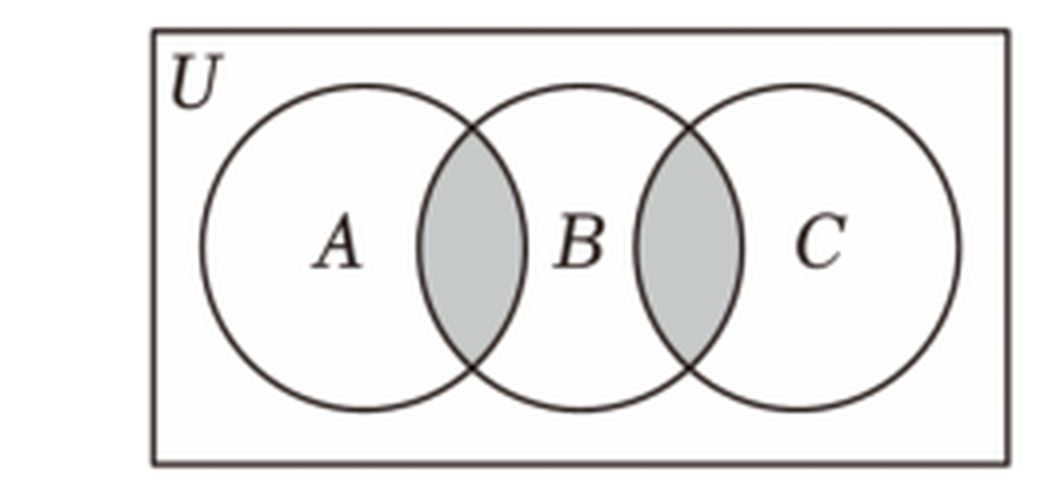
\includegraphics[width=0.30\textwidth]{figures/venn_ABC_lenses.png}
\end{center}

\keepwithprev
A. $B\cap(A\cup C)$\qquad\qquad\qquad B. $B\cap(A\cap C)$

C. $B\cap\complement_U(A\cup C)$\qquad\qquad D. $(A\cup B)\cap(B\cup C)$

\ans{$A$}

\ifanswer
\solbegin
\step{由图中阴影部分得，阴影为集合 $A$、$B$ 的交集和 $B$、$C$ 的交集的并集，}
\step{故阴影部分可表示为 $(A\cap B)\cup(B\cap C)$ 或 $B\cap(A\cup C)$，
故 $A$ 正确. 故选 $A$.}
\solend

\fi

\item 设集合 $P_1=\{x\mid x^2+ax+1>0\}$，$P_2=\{x\mid x^2+ax+2>0\}$，
$Q_1=\{x\mid x^2+x+b>0\}$，$Q_2=\{x\mid x^2+2x+b>0\}$，其中 $a$、$b\in\R$，
对于下列两个命题：①存在 $a$，$P_1$ 不是 $P_2$ 的子集；②存在 $b$ 使得 $Q_1$ 是 $Q_2$
的子集. 下列说法正确的是\mbox{（\quad）}

\keepwithprev
A. ①是真命题，②是假命题\qquad B. ①是假命题，②是真命题

C. ①②都是真命题\qquad\qquad\quad D. ①②都是假命题

\ans{$B$}

\ifanswer
\solbegin
\step{对于集合 $P_1=\{x\mid x^2+ax+1>0\}$，$P_2=\{x\mid x^2+ax+2>0\}$，}
\step{得当 $m\in P_1$ 时，即 $m^2+am+1>0$，得 $m^2+am+2>0$，}
\step{即有 $m\in P_2$，得对任意 $a$，$P_1$ 是 $P_2$ 的子集，故①错误；}
\step{对于集合 $Q_1=\{x\mid x^2+x+b>0\}$，$Q_2=\{x\mid x^2+2x+b>0\}$，}
\step{当 $b=6$ 时，$Q_1=\{x\mid x^2+x+6>0\}=\R$，$Q_2=\{x\mid x^2+2x+6>0\}=\R$，}
\step{得 $Q_1$ 是 $Q_2$ 的子集，所以存在 $b$，使得 $Q_1$ 是 $Q_2$ 的子集，故②正确；}
\step{故选 $B$.}
\solend

\fi

\item 设 $a$、$b\in\R$，则“$a+b>2$ 且 $ab>1$”是“$a>1$ 且 $b>1$”的\mbox{（\quad）}

\keepwithprev
A. 充要条件\qquad\qquad\qquad B. 充分不必要条件

C. 必要不充分条件\qquad\quad D. 既不充分又不必要条件

\ans{$C$}

\ifanswer
\solbegin
\step{因为 $a>1$ 且 $b>1$，所以 $a+b>2$ 且 $ab>1$，}
\step{若已知 $a+b>2$ 且 $ab>1$，可取 $a=\dfrac12$，$b=8$，也满足已知，}
\step{所以“$a+b>2$ 且 $ab>1$”是“$a>1$ 且 $b>1$”的必要不充分条件，故选 $C$.}
\solend

\fi

\item 十七世纪，数学家费马提出猜想：“对任意正整数 $n>2$，关于 $x$、$y$、$z$ 的方程
$x^n+y^n=z^n$ 没有正整数解”. 1995 年数学家安德鲁·怀尔斯发表了完成的证明过程，使它
终成费马大定理. 对费马大定理，若用反证法证明，第一步是假设猜想不成立，即\mbox{（\quad）}

\keepwithprev
A. 对任意正整数 $n>2$，关于 $x$、$y$、$z$ 的方程 $x^n+y^n=z^n$ 都有正整数解

B. 对任意正整数 $n>2$，关于 $x$、$y$、$z$ 的方程 $x^n+y^n=z^n$ 至少存在一组正整数解

C. 存在正整数 $n\leqslant2$，关于 $x$、$y$、$z$ 的方程 $x^n+y^n=z^n$ 至少存在一组正整数解

D. 存在正整数 $n>2$，关于 $x$、$y$、$z$ 的方程 $x^n+y^n=z^n$ 至少存在一组正整数解

\ans{$D$}

\end{enumerate}

\bigsec{三、解答题}

\begin{enumerate}
\setcounter{enumi}{16}

\item 已知 $a$、$b$、$c$ 都是实数，且 $a+b+c=0$，$abc=1$，求证：$a$、$b$、$c$ 中必有一个
大于 $\dfrac32$.

\ifanswer
\solbegin
\step{由 $a+b+c=0$，$abc=1$，得 $a$、$b$、$c$ 中一个正数，两个负数，}
\step{不妨设 $c>0$，由题意得 $a+b=-c,ab=\dfrac1c$，}
\step{由根与系数的关系得 $a$、$b$ 是关于 $x$ 的方程 $x^2+cx+\dfrac1c=0$ 的两个根，}
\step{则 $\Delta=c^2-\dfrac4c=\dfrac{c^3-4}{c}\geqslant0$，}
\step{因为 $c>0$，所以 $c^3\geqslant4$，得 $c\geqslant\sqrt[3]{4}$，}
\step{又 $\dfrac32=\sqrt[3]{\left(\dfrac32\right)^3}=\sqrt[3]{\dfrac{27}{8}}<\sqrt[3]{4}$，}
\step{所以 $c>\dfrac32$，即 $a$、$b$、$c$ 中必有一个大于 $\dfrac32$.}
\solend

\fi

\ansspace[6]

\item 已知关于 $x$ 的一元二次方程 $x^2-mx+4m^2-3=0$ 的两个实根分别为 $x_1,x_2$.

\begin{enumerate}[label=(\arabic*)]
\item $x_1,x_2$ 均为正根，求实数 $m$ 的取值范围；
\item 若 $x_1,x_2$ 满足：$x_1+x_2=x_1x_2$，求实数 $m$ 的值.
\end{enumerate}

\ifanswer
\solbegin
\stepm{(1)}{由 $x_1,x_2$ 均为正根，得}
\step{$\begin{cases}\Delta=(-m)^2-4(4m^2-3)\geqslant0\\ x_1+x_2=m>0\\ x_1\cdot x_2=4m^2-3>0\end{cases}$，}
\step{解得 $\begin{cases}-\dfrac{2\sqrt5}{5}\leqslant m\leqslant\dfrac{2\sqrt5}{5}\\[4pt]
m>0\\[4pt] m\leqslant-\dfrac{\sqrt3}{2}$ 或 $m\geqslant\dfrac{\sqrt3}{2}\end{cases}$，}
\step{即 $\dfrac{\sqrt3}{2}\leqslant m\leqslant\dfrac{2\sqrt5}{5}$；}
\stepm{(2)}{由 (1) 得
$\begin{cases}-\dfrac{2\sqrt5}{5}\leqslant m\leqslant\dfrac{2\sqrt5}{5}\\[4pt]
m=4m^2-3\end{cases}$，解得 $m=1$（舍去）或 $m=-\dfrac34$，}
\step{则 $m=-\dfrac34$.}
\solend

\fi

\ansspace[6]

\item 已知集合 $A=\{x\mid m-1<x<m^2+1\}$，$B=\{x\mid-2<x<2\}$.

\begin{enumerate}[label=(\arabic*)]
\item 当 $m=2$ 时，求 $A\cup B$、$A\cap B$、$\complement_R B$、$A\cap(\complement_R B)$；
\item 若“$x\in A$”是“$x\in B$”成立的必要不充分条件，求实数 $m$ 的取值范围.
\end{enumerate}

\ifanswer
\solbegin
\stepm{(1)}{$m=2$ 时，$A=\{x\mid1<x<5\}$，且 $B=\{x\mid-2<x<2\}$，}
\step{所以 $A\cup B=\{x\mid-2<x<5\}$，$A\cap B=\{x\mid1<x<2\}$，}
\step{$\complement_R B=\{x\mid x\leqslant-2$ 或 $x\geqslant2\}$，
$A\cap(\complement_R B)=\{x\mid2\leqslant x<5\}$；}
\stepm{(2)}{若“$x\in A$”是“$x\in B$”成立的必要不充分条件，则 $B\subset A$，}
\step{所以 $\begin{cases}m-1<-2\\ m^2+1\geqslant2\end{cases}$
或 $\begin{cases}m-1\leqslant-2\\ m^2+1>2\end{cases}$，解得 $m<-1$，}
\step{故 $m$ 的取值范围为 $(-\infty,-1)$.}
\solend

\fi

\ansspace[6]

\item 已知 $m\in\R$，集合 $A=\{x\mid|x-1|\leqslant2\}$，集合
$B=\{x\mid m-3<x\leqslant m+2\}$.

\begin{enumerate}[label=(\arabic*)]
\item 若“$x\in A$”是“$x\in B$”的充分不必要条件，求 $m$ 的取值范围；
\item 若命题“$\forall x\in B$，$x\in\complement_R A$”是真命题，求 $m$ 的取值范围；
\item 若命题“$\exists x\in A$，$x\in B$”是真命题，求 $m$ 的取值范围.
\end{enumerate}

\ifanswer
\solbegin
\stepm{(1)}{集合 $A=\{x\mid|x-1|\leqslant2\}=\{x\mid-1\leqslant x\leqslant3\}$，}
\step{若“$x\in A$”是“$x\in B$”的充分不必要条件，则 $A\subset B$，}
\step{所以 $\begin{cases}m-3<-1\\ 3\leqslant m+2\end{cases}$，解得 $1\leqslant m<2$，}
\step{当 $m=1$ 时，$B=\{x\mid-2<x\leqslant3\}$，符合题意，}
\step{所以 $m$ 的取值范围是 $\{m\mid1\leqslant m<2\}$.}
\stepm{(2)}{若命题“$\forall x\in B$，$x\in\complement_R A$”是真命题，则 $B\subset\complement_R A$，}
\step{又 $\complement_R A=\{x\mid x<-1$ 或 $x>3\}$，$B\neq\varnothing$，
所以 $m+2<-1$ 或 $m-3\geqslant3$，}
\step{解得 $m<-3$ 或 $m\geqslant6$，所以 $\{m\mid m<-3$ 或 $m\geqslant6\}$；}
\stepm{(3)}{因为 $\exists x\in A$，$x\in B$ 是真命题，所以 $A\cap B\neq\varnothing$，}
\step{当 $A\cap B=\varnothing$ 时，所以 $m+2<-1$ 或 $m-3\geqslant3$，
即 $m<-3$ 或 $m\geqslant6$，}
\step{所以当 $A\cap B\neq\varnothing$ 时，$m$ 的取值范围是 $\{m\mid-3\leqslant m<6\}$，}
\step{则 $m$ 的取值范围是 $\{m\mid-3\leqslant m<6\}$.}
\solend

\fi

\ansspace[6]

\item 对于函数 $f(x)$，若 $f(x_0)=x_0$，则称 $x_0$ 为 $f(x)$ 的“不动点”；若
$f[f(x_0)]=x_0$，则称 $x_0$ 为 $f(x)$ 的“稳定点”. 函数 $f(x)$ 的“不动点”和“稳定点”
的集合分别记为 $A$ 和 $B$，即 $A=\{x\mid f(x)=x\}$，$B=\{x\mid f[f(x)]=x\}$.

\begin{enumerate}[label=(\arabic*)]
\item 设函数 $f(x)=3x+4$，求集合 $A$ 和 $B$；
\item 求证：$A\sub B$；
\item 设函数 $f(x)=ax^2+bx+c(a\neq0)$，且 $A=\varnothing$，求证：$B=\varnothing$.
\end{enumerate}

\ifanswer
\solbegin
\stepm{(1)}{令 $f(x)=3x+4=x$，解得 $x=-2$，故有 $A=\{-2\}$，}
\step{由于 $f[f(x)]=3(3x+4)+4=9x+16$，}
\step{令 $9x+16=x$，得 $x=-2$，故有 $B=\{-2\}$；}
\stepm{(2)}{若 $A=\varnothing$，则 $A\sub B$ 显然成立；}
\step{若 $A\neq\varnothing$，设 $t\in A$，则 $f(t)=t$，$f(f(t))=f(t)=t$，}
\step{所以 $t\in B$，故 $A\sub B$.}
\stepm{(3)}{因为 $A=\{x\mid f(x)=x\}=\varnothing$，所以 $ax^2+bx+c=x$ 无解，}
\step{即 $\Delta=(b-1)^2-4a<0$，}
\step{①当 $a>0$ 时，二次函数 $y=f(x)-x$，}
\step{即 $y=ax^2+(b-1)x+c$ 的图象在 $x$ 轴的上方，}
\step{所以 $\forall x\in\R$，$f(x)-x>0$ 恒成立，所以 $\forall x\in\R$，
$f(x)>x$ 恒成立，}
\step{所以 $\forall x\in\R$，$f[f(x)]>f(x)>x$ 恒成立，即 $B=\varnothing$；}
\step{②当 $a<0$ 时，同理可证 $B=\varnothing$；}
\step{综上，对于函数 $f(x)=ax^2+bx+c(a\neq0)$，当 $A=\varnothing$ 时，$B=\varnothing$.}
\solend

\fi

\ansspace*[10]

\end{enumerate}

\end{document}
